\documentclass[11pt, a4paper]{book}
\usepackage{graphicx} 
\usepackage{}
\usepackage[toc,page]{appendix}
\usepackage[square,sort,comma,numbers]{natbib}
\usepackage[pdftex,usenames,dvipsnames]{color}
\usepackage{paralist}
\usepackage{tabularx}
\usepackage{pdfpages}
\newcommand{\VUnits} {\ensuremath{V_{units}}}
\newcommand{\VPegs} {\ensuremath{V_{pegs}}}
\newcommand{\Constraints}[2] {\ensuremath{C_{v_{#1},v_{#2}}}}
\newcommand{\Cons}[5] {\ensuremath{C_{v_{#1},v_{#2},v_{#3},v_{#4},v_{#5}}}}
\newcommand{\Con}[3] {\ensuremath{C_{v_{#1},v_{#2},v_{#3}}}}
\newcommand{\Const}[4] {\ensuremath{C_{v_{#1},v_{#2},v_{#3},v_{#4}}}}
\newcommand{\Constraint}[1] {\ensuremath{C_{v_{#1}}}}
\newcommand{\Domain}[1] {\ensuremath{D(v_{#1})}}
\newcommand*\circled[1]{\tikz[baseline=(char.base)]{
            \node[shape=circle,draw,inner sep=2pt] (char) {#1};}}
%%%%%%%%%%%%%%%%%%%%%%%%%%%%%%%%%%%%%%%%%%%%%%%%%%%%%%%%%%%%%%%%%%%%%%%%%%%%%%%%
% Packages                                                                     %
%%%%%%%%%%%%%%%%%%%%%%%%%%%%%%%%%%%%%%%%%%%%%%%%%%%%%%%%%%%%%%%%%%%%%%%%%%%%%%%%

% thesis %%%%%%%%%%%%%%%%%%%%%%%%%%%%%%%%%%%%%%%%%%%%%%%%%%%%%%%%%%%%%%%%%%%%%%%
% uses palatino for body (serif) text; other options: cm, lucida, times, minionpro
\usepackage[palatino]{anuthesis}

% footers %%%%%%%%%%%%%%%%%%%%%%%%%%%%%%%%%%%%%%%%%%%%%%%%%%%%%%%%%%%%%%%%%%%%%%
%\usepackage[draft]{prelim2e}
\usepackage[final]{prelim2e}  % use this version to disable the footer
\renewcommand{\PrelimWords}{\textbf{DRAFT}}

% bibliography %%%%%%%%%%%%%%%%%%%%%%%%%%%%%%%%%%%%%%%%%%%%%%%%%%%%%%%%%%%%%%%%%
\usepackage[square]{natbib}

% fonts %%%%%%%%%%%%%%%%%%%%%%%%%%%%%%%%%%%%%%%%%%%%%%%%%%%%%%%%%%%%%%%%%%%%%%%%
% If you get an error about missing these packages, you need to update your
% LaTeX distribution. These fonts are both included in the latest TeXlive/MacTex
% 2013 distributions. Alternatively, follow the instructions in readme.fonts.txt
% to get Optima installed, or find your own sans-serif font!
\usepackage[T1]{fontenc}
\usepackage[scaled]{PTSans}          % use Paratype Sans for sans-serif
%\renewcommand*\sfdefault{uop}        % use Optima for sans-serif, see readme.fonts.txt
\usepackage[scaled]{DejaVuSansMono}  % use DejaVu Sans Mono for monospace

% nicer text layout %%%%%%%%%%%%%%%%%%%%%%%%%%%%%%%%%%%%%%%%%%%%%%%%%%%%%%%%%%%%
\usepackage[stretch=10,shrink=10]{microtype}
%\setstretch{1.1}  % to increase line spacing

% math %%%%%%%%%%%%%%%%%%%%%%%%%%%%%%%%%%%%%%%%%%%%%%%%%%%%%%%%%%%%%%%%%%%%%%%%%
\usepackage{amsmath}
\usepackage{amssymb}

% figures %%%%%%%%%%%%%%%%%%%%%%%%%%%%%%%%%%%%%%%%%%%%%%%%%%%%%%%%%%%%%%%%%%%%%%
\usepackage{graphicx}
\usepackage[table]{xcolor}
\usepackage{float}

% captions %%%%%%%%%%%%%%%%%%%%%%%%%%%%%%%%%%%%%%%%%%%%%%%%%%%%%%%%%%%%%%%%%%%%%
% for sans-serif captions, change font=small to font={small,sf}
\usepackage{caption}
\usepackage{subcaption}
\captionsetup[figure]{labelsep=colon,font=small,labelfont=bf}
\captionsetup[subfigure]{format=plain,labelformat=simple,labelfont={}}
\captionsetup[table]{labelsep=colon,font=small,labelfont=bf}
\renewcommand\thesubfigure{(\alph{subfigure})}  % format subfigure captions like (a)

% tables %%%%%%%%%%%%%%%%%%%%%%%%%%%%%%%%%%%%%%%%%%%%%%%%%%%%%%%%%%%%%%%%%%%%%%%
\usepackage{booktabs}
\usepackage{relsize}
\usepackage{multirow}
\usepackage{array}
\renewcommand{\arraystretch}{1.2}  % stretch space between table rows a bit

% code %%%%%%%%%%%%%%%%%%%%%%%%%%%%%%%%%%%%%%%%%%%%%%%%%%%%%%%%%%%%%%%%%%%%%%%%%
\usepackage{listings}

% enumerations %%%%%%%%%%%%%%%%%%%%%%%%%%%%%%%%%%%%%%%%%%%%%%%%%%%%%%%%%%%%%%%%%
\usepackage{enumitem}

% todo notes %%%%%%%%%%%%%%%%%%%%%%%%%%%%%%%%%%%%%%%%%%%%%%%%%%%%%%%%%%%%%%%%%%%
\definecolor{todocolor}{rgb}{0.8,0.8,1.0}
\usepackage[color=todocolor,colorinlistoftodos]{todonotes}

% SI units %%%%%%%%%%%%%%%%%%%%%%%%%%%%%%%%%%%%%%%%%%%%%%%%%%%%%%%%%%%%%%%%%%%%%
\usepackage[binary-units=true]{siunitx}

% misc %%%%%%%%%%%%%%%%%%%%%%%%%%%%%%%%%%%%%%%%%%%%%%%%%%%%%%%%%%%%%%%%%%%%%%%%%
\usepackage{xspace}
\usepackage{afterpage}
\usepackage[normalem]{ulem}
\usepackage{makeidx}
\usepackage{url}
\urlstyle{sf}

% display landscape pages as landscape in PDF
\usepackage{pdflscape}
% PDF links %%%%%%%%%%%%%%%%%%%%%%%%%%%%%%%%%%%%%%%%%%%%%%%%%%%%%%%%%%%%%%%%%%%%
\PackageWarning{report template}{Update your PDF title and author!} % delete this line when done
\usepackage[
  hyperindex=true,
  bookmarks=true,
  pdftitle={YOUR TITLE HERE},
  pdfauthor={YOUR NAME HERE},
  colorlinks=false,
  plainpages=false,
  pdfborder={0 0 0},
  pdfpagelabels,
  hyperfootnotes=false]{hyperref}
\usepackage[all]{hypcap}  % fix links to figures to point to top not bottom

% backreferences in bibliography %%%%%%%%%%%%%%%%%%%%%%%%%%%%%%%%%%%%%%%%%%%%%%%
% e.g. "(cited on page 12)". Comment out this whole section to disable.
\usepackage[hyperpageref]{backref}
\renewcommand*{\backref}[1]{}
\renewcommand*{\backrefalt}[4]{
  \ifcase #1 %
    %
  \or
    (cited on page #2)%
  \else
    (cited on pages #2)%
  \fi
}

% clever cross-refs %%%%%%%%%%%%%%%%%%%%%%%%%%%%%%%%%%%%%%%%%%%%%%%%%%%%%%%%%%%%
\usepackage[nameinlink,capitalise]{cleveref}

%%%%%%%%%%%%%%%%%%%%%%%%%%%%%%%%%%%%%%%%%%%%%%%%%%%%%%%%%%%%%%%%%%%%%%%%%%%%%%%%
% Setup
%%%%%%%%%%%%%%%%%%%%%%%%%%%%%%%%%%%%%%%%%%%%%%%%%%%%%%%%%%%%%%%%%%%%%%%%%%%%%%%%

% doi links
\newcommand{\doi}[1]{\href{http://dx.doi.org/#1}{\nolinkurl{doi:#1}}}

% code listings
\lstloadlanguages{java}
\lstdefinestyle{default}{
  numbers=left,
  numberstyle=\tiny,
  stepnumber=1,
  numbersep=2em,
  language=java,                         % the language
  basicstyle=\footnotesize\ttfamily,     % the basic font family to use
  commentstyle=\itshape,                 % the font for comments
  stringstyle=\ttfamily,
}
\lstset{style=default}

% references to lines of code
\lstset{escapeinside={(*@}{@*)}}
\crefname{line}{line}{lines}  % cleveref wants to capitalise "Line" mid-sentence

% figures
\DeclareGraphicsRule{*}{pdf}{*}{}

% tables
\newcommand{\otoprule}{\midrule[\heavyrulewidth]}
\definecolor{tableheadcolor}{rgb}{0.8,0.8,1.0}
\definecolor{tablealtcolor}{rgb}{0.9,0.9,0.95}

% bold table rows (use \rowstyle{\bffamily} on each bold row)
\newcolumntype{B}{>{\global\let\currentrowstyle\relax}}
\newcolumntype{^}{>{\currentrowstyle}}
\newcommand{\rowstyle}[1]{\gdef\currentrowstyle{#1}#1\ignorespaces}
\newcolumntype{C}{>{\bfseries}}

% sans-serif tables
\let\oldtabular\tabular
\let\endoldtabular\endtabular
\renewenvironment{tabular}{\sffamily\oldtabular}{\endoldtabular}

% bibliography - make heading lowercase
\makeatletter
\renewcommand\bibsection{%
      \chapter*{\bibname\@mkboth{\bibname}{\bibname}}}
\makeatother

% use computer modern for mathbb -- the palatino blackboard font is ugly as sin
\AtBeginDocument{
  \DeclareSymbolFont{AMSb}{U}{msb}{m}{n}
  \DeclareSymbolFontAlphabet{\mathbb}{AMSb}}

%%%%%%%%%%%%%%%%%%%%%%%%%%%%%%%%%%%%%%%%%%%%%%%%%%%%%%%%%%%%%%%%%%%%%%%%%%%%%%%%
% Basic macros                                                                 %
%%%%%%%%%%%%%%%%%%%%%%%%%%%%%%%%%%%%%%%%%%%%%%%%%%%%%%%%%%%%%%%%%%%%%%%%%%%%%%%%

% Inline code %%%%%%%%%%%%%%%%%%%%%%%%%%%%%%%%%%%%%%%%%%%%%%%%%%%%%%%%%%%%%%%%%%
% use like: "The \icode{Geocoordinate} class specifies ..."
\newcommand{\icode}[1]{{\lstset{basicstyle=\ttfamily\small}\lstinline@#1@}}

% Todo notes %%%%%%%%%%%%%%%%%%%%%%%%%%%%%%%%%%%%%%%%%%%%%%%%%%%%%%%%%%%%%%%%%%%
\definecolor{fixcolor}{rgb}{1,0.8,0.8}
\newcommand{\fix}[1]{\todo[color=fixcolor]{#1}\xspace}
\newcommand{\ifix}[1]{\todo[inline,color=fixcolor]{#1}}
\definecolor{commentcolor}{rgb}{0.8,1.0,0.8}
\newcommand{\comment}[1]{\todo[color=commentcolor]{#1}}
\newcommand{\icomment}[1]{\todo[inline,color=commentcolor]{#1}}
\newcommand{\itodo}[1]{\todo[inline]{#1}}

%%%%%%%%%%%%%%%%%%%%%%%%%%%%%%%%%%%%%%%%%%%%%%%%%%%%%%%%%%%%%%%%%%%%%%%%%%%%%%%%
% Your macros                                                                  %
%%%%%%%%%%%%%%%%%%%%%%%%%%%%%%%%%%%%%%%%%%%%%%%%%%%%%%%%%%%%%%%%%%%%%%%%%%%%%%%%

% Here's an example abbreviation macro. Notice the \xspace at the end, to ensure
% it gets the right spacing after it.
\newcommand{\jikesrvm}{Jikes RVM\xspace}
% We can also make things sans-serif, which might be better style.
\newcommand{\avrora}{\textsf{avrora}\xspace}

\definecolor{ForestGreen}{RGB}{34,106,46}

\lstdefinelanguage{minizinc}{
    morekeywords={
        %% MiniZinc keywords
        %%
        ann, annotation, any, array, assert,
        bool,
        constraint,
        else, elseif, endif, enum, exists,
        float, forall, function,
        if, in, include, int,
        list,
        minimize, maximize,
        of, op, output,
        par, predicate,
        record,
        set, solve, string,
        test, then, tuple, type,
        var,
        where,
        %% MiniZinc functions
        %%
        abort, abs, acosh, array_intersect, array_union,
        array1d, array2d, array3d, array4d, array5d, array6d, asin, assert, atan,
        bool2int,
        card, ceil, combinator, concat, cos, cosh,
        dom, dom_array, dom_size, dominance,
        exp,
        fix, floor,
        index_set, index_set_1of2, index_set_2of2, index_set_1of3, index_set_2of3, index_set_3of3,
        int2float, is_fixed,
        join,
        lb, lb_array, length, let, ln, log, log2, log10,
        min, max,
        pow, product,
        round,
        set2array, show, show_int, show_float, sin, sinh, sqrt, sum,
        tan, tanh, trace,
        ub, and ub_array,
        %% Search keywords
        %%
        bool_search, int_search, seq_search, priority_search,
        %% MiniSearch keywords
        %%
        minisearch, search, while, repeat, next, commit, print, post, sol, scope, time_limit, break, fail
    },
    sensitive=true, % are the keywords case sensitive
    morecomment=[l][\em\color{ForestGreen}]{\%},
    %morecomment=[s]{/*}{*/},
    morestring=[b]",
}
%% Settings for listings
%%
\lstset{ %
    backgroundcolor=\color{lightgray!40},  % choose the background color; you must add
                                        % \usepackage{color} or \usepackage{xcolor}
    basicstyle=\scriptsize\ttfamily,    % the size of the fonts that are used for the code
    belowskip=-2em,
    breakatwhitespace=false,            % sets if automatic breaks should only happen at whitespace
    breaklines=true,                    % sets automatic line breaking
    captionpos=b,                       % sets the caption-position to bottom
    commentstyle=\color{ForestGreen},   % comment style
    %deletekeywords={...},              % if you want to delete keywords from the given language
    escapeinside={\%*}{*)},             % if you want to add LaTeX within your code
    extendedchars=true,                 % lets you use non-ASCII characters; for 8-bits
                                        % encodings only, does not work with UTF-8
    frame=single,                       % adds a frame around the code
    keepspaces=true,                    % keeps spaces in text, useful for keeping indentation
                                        % of code (possibly needs columns=flexible)
    keywordstyle=\bfseries\color{blue}, % keyword style
    language=minizinc,                  % the language of the code
    %morekeywords={*,...},              % if you want to add more keywords to the set
    numbers=left,                       % where to put the line-numbers; possible values are (none, left, right)
    %numbersep=5pt,                     % how far the line-numbers are from the code
    %numberstyle=\tiny\color{Gray},     % the style that is used for the line-numbers
    rulecolor=\color{black},            % if not set, the frame-color may be changed
                                        % on line-breaks within not-black text (e.g. comments (green here))
    showspaces=false,                   % show spaces everywhere adding particular
                                        % underscores; it overrides 'showstringspaces'
    showstringspaces=false,             % underline spaces within strings only
    showtabs=false,                     % show tabs within strings adding particular underscores
    %stepnumber=1,                      % the step between two line-numbers. If it's 1, each line will be numbered
    stringstyle=\color{Red},            % string literal style
    tabsize=2,                          % sets default tabsize to 2 spaces
    title=\lstname                      % show the filename of files included with \lstinputlisting;
                                        % also try caption instead of title
}
\allowdisplaybreaks
%%%%%%%%%%%%%%%%%%%%%%%%%%%%%%%%%%%%%%%%%%%%%%%%%%%%%%%%%%%%%%%%%%%%%%%
%% Preamble
\title{Solving Puzzle Games with CSP Solvers}
\author{Mingzhen Ao}
\date{\today}

\renewcommand{\thepage}{\roman{page}}

\makeindex
\begin{document}

%%%%%%%%%%%%%%%%%%%%%%%%%%%%%%%%%%%%%%%%%%%%%%%%%%%%%%%%%%%%%%%%%%%%%%%
%% Title page
\pagestyle{empty}
\thispagestyle{empty}
\begin{titlepage}
  \enlargethispage{2cm}
  \begin{center}
    \makeatletter
    \Huge\textbf{\@title} \\[.4cm]
    \Huge\textbf{\thesisqualifier} \\[2.5cm]
    \huge\textbf{\@author} \\[9cm]
    \makeatother
    \LARGE A report submitted for the course \\
    COMP8755 Individual Computing Project \\
    Supervised by: Pascal Bercher and Florian Geißer
    
    The Australian National University \\[2cm]
    \thismonth
    
    \vspace*{\fill}
    \makeatletter
        {\fontfamily{lmr}\selectfont\textcopyright}\ \@author{} \number\year
        \makeatother
   
    
  \end{center}
\end{titlepage}


%%%%%%%%%%%%%%%%%%%%%%%%%%%%%%%%%%%%%%%%%%%%%%%%%%%%%%%%%%%%%%%%%%%%%%%
%% Here begin the preliminaries
\vspace*{7cm}
\begin{center}
  Except where otherwise indicated, this report is my own original
  work.
\end{center}

\vspace*{4cm}

\hspace{8cm}\makeatletter\@author\makeatother\par
\hspace{8cm}\today


%%%%%%%%%%%%%%%%%%%%%%%%%%%%%%%%%%%%%%%%%%%%%%%%%%%%%%%%%%%%%%%%%%%%%%%
%% Acknowledgements
\cleardoublepage
\pagestyle{empty}
\chapter*{Acknowledgments}
\addcontentsline{toc}{chapter}{Acknowledgments}
Who do you want to thank? I hope it includes your supervisor(s).


%%%%%%%%%%%%%%%%%%%%%%%%%%%%%%%%%%%%%%%%%%%%%%%%%%%%%%%%%%%%%%%%%%%%%%%
%% Abstract
\cleardoublepage
\pagestyle{headings}
\chapter*{Abstract}
\addcontentsline{toc}{chapter}{Abstract}
\vspace{-1em}
The constraint satisfaction problems (CSPs) are created to model two puzzle games IQ Twist and Zig Zag Puzzler. Both of them have "start", "junior", "expert", "master" and "wizard" difficulties. With regard to CSPs for both games, the variables, domains, and constraints are mainly discussed. Meanwhile, in the process of discussing constraints, the 2D rotation matrix is introduced to clarify the pieces' configurations for the 2D game (IQ Twist), and the 3D rotation matrix is introduced to clarify the pieces' configurations for the 3D game (Zig Zag Puzzler). After that, these models are encoded by Minizinc which is a constraint modeling language. Through Minizinc IDE, the Minizinc is transferred to Flatzinc, a solver input language that is understood by a wide range of solvers. Therefore, nine solvers are used to execute these problems by different interfaces, which create the bridges between each solver and the Flatzinc file. For IQ Twist, the solvers' performances are not strongly related to the difficulties, while there is an obvious negative correlation between the performance and difficulties in Zig Zag Puzzler. Finally, there are three solvers Chuffed, OR-Tools and PicatSAT, which perform the 100 percent coverage. In other words,  they solve each problem in thirty minutes. More specifically, Chuffed achieve the optimal performance in most problems because it solves each problem in 20 seconds, while the other two need more time.
\\
\\
\\
\\\textbf{Keywords:} CSPs, IQ Twist, Zig Zag Puzzler, rotation matrix, Minizinc, Flatzinc, Chuffed, OR-Tools, PicatSAT.




%%%%%%%%%%%%%%%%%%%%%%%%%%%%%%%%%%%%%%%%%%%%%%%%%%%%%%%%%%%%%%%%%%%%%%%
%% Table of contents
\cleardoublepage
\microtypesetup{protrusion=false}  % make sure numbers align in TOC
\pagestyle{headings}
\markboth{Contents}{Contents}
\tableofcontents
\listoffigures
\listoftables
\microtypesetup{protrusion=true}

%%%%%%%%%%%%%%%%%%%%%%%%%%%%%%%%%%%%%%%%%%%%%%%%%%%%%%%%%%%%%%%%%%%%%%
%% Here begins the main text
\mainmatter

%% Introduction
\chapter{Introduction}
\label{cha:intro}
\section{Thesis Statement}
\label{sec:problemstatement}
The goal of this project is to model two puzzle games based on CSPs and compare the performances of different solvers to solve these problems.
\section{Introduction}
\label{sec:introduction}
In March 2016, AlphaGo played Go with Lee Sedol who is one of the best Go players in the world, after five games in a week, AlphaGo wins the series 4:1~\cite{r26}. A computer program defeats the best player in the world, which indicates that the computer takes huge advantages compared with the human in such a game that contains a finite of possible situations. Hence, the effective use of the computer can significantly accelerate the speed of solving some problems. A mathematical model like a CSP can be a bridge that connects the real-world problem with the computer. Through the bridge, the computer can help human solves problems in real life. CSP has been developed in a long history, it originated in the field of artificial intelligence in 1978 by Jena-LonisLauriere~\cite{r27}. At that time, it was limited to computing power so that it's hard to solve the problems with high complexity within a reasonable time. The performance may be worse than the performance of human solving it. However, with the development of optimization methods and the growth of computing power, it has been widely used to solve some complex problems in many aspects such as location, scheduling, car sequencing, vehicle routing, timetabling, rostering and so on~\cite{r28}. Meanwhile, along with the wide applications of CSPs, many compilers have supported the constraint satisfaction programming language. And massive researchers in the world have created different solvers that adopt different optimization methods to solve such a problem. Due to the different features of the solvers, the performance of each solver to different problems may have an obvious difference. Therefore, the comparisons between them are meaningful because it helps the modeler to choose the suitable one.
\section{Thesis Outline}
\label{sec:outline}
In this thesis, some basic background knowledge such as CSP, rotation matrix and Minizinc Language are introduced in Chapter~\ref{cha:background}. The details of CSP models and corresponding encodings in Minizinc for both IQ Twist and Zig Zag Puzzler are presented in Chapter~\ref{cha:design}. In Chapter~\ref{cha:evaluation}, there is a discussion about the experiment results of nine different solvers. Moreover, the conclusion and future work is described in Chapter~\ref{cha:conc}.


%% Chapters
\chapter{Background and Related Work}
\label{cha:background}

At the beginning of each chapter, please give the motivation and
high-level picture of the chapter. You also have to introduce the sections
in the chapter, e.g.\

  Section~\ref{sec:background} gives background material necessary in
  order to read this report ,and related work is given in
  Section~\ref{sec:relatedwork}.\\

  
\section{Background}
\label{sec:background}


\section{Related work}
\label{sec:relatedwork}

You may reference other papers. For example: Generational garbage
collection~\citep{LH:83,Moon:84,Ungar:84} is perhaps the single most
important advance in garbage collection since the first collectors
were developed in the early 1960s. (doi: "doi" should just be the doi
part, not the full URL, and it will be made to link to dx.doi.org and
resolve.  shortname: gives an optional short name for a conference
like PLDI '08.)


\section{Summary}

Summarize what you discussed in this chapter, and introduce the story
of next chapter. Readers should roughly understand what your report
talks about by only reading words at the beginning and the end
(Summary) of each chapter.



\chapter{CSP Models for Puzzle Games}
\label{cha:design}
Generally, this chapter discusses three parts: the CSP model for 2D game (IQ Twist), the CSP models for the two playing modes of 3D game (ZIG ZAG Puzzler) and the implementations of all models.
\section{IQ Twist}
IQ Twist is a puzzle game which consists of 8 twisted puzzle pieces and 7 coloured pegs (Figure~\ref{fig:IQ_twist_game}). To play the game, the colored pegs should be placed on the board, then fit all the twisted puzzle pieces back into the board. Different units of pieces must match the pegs with the same color and only the hollow units of piece can be used to match pegs. The degree of difficulty can be adjusted by the placements of pegs.
\begin{figure}[htbp]
    \centering
    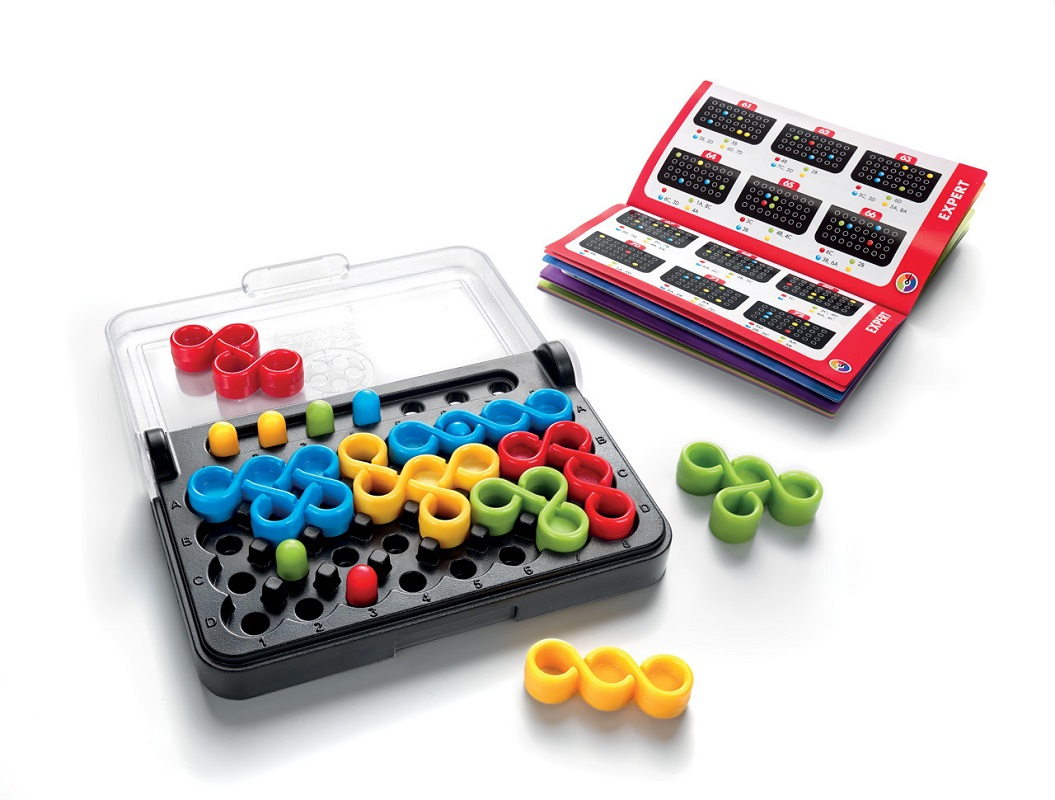
\includegraphics[width=0.5\textwidth]{figs/IQtwistintroduction.jpg}
    \caption{IQ Twist game, adopted from~\cite{r21}}
    \label{fig:IQ_twist_game}
\end{figure}
\subsection{Variables}
Above all, the initial state of each piece is defined in Figure~\ref{fig:allinit}.
\begin{figure}[htbp]
\begin{subfigure}[b]{.24\textwidth}
\centering

\includegraphics[width=0.75\textwidth]{figs/yellow1.jpg}
\caption{Initial state of yellow1}
  \label{fig:2Dyellow1}
\end{subfigure}
\begin{subfigure}[b]{.24\textwidth}
\centering

\includegraphics[width=0.75\textwidth]{figs/yellow2.jpg}
\caption{Initial state of yellow2}
  \label{fig:2Dyellow2}
\end{subfigure}
\begin{subfigure}[b]{.24\textwidth}
\centering

\includegraphics[width =0.5\textwidth]{figs/blue1.jpg}
\caption{Initial state of blue1}
  \label{fig:2Dblue1}
\end{subfigure}
\begin{subfigure}[b]{.24\textwidth}
\centering

\includegraphics[width=\textwidth]{figs/blue2.jpg}
\caption{Initial state of blue2}
  \label{fig:2Dblue2}
\end{subfigure}
\begin{subfigure}[b]{.24\textwidth}
\centering

\includegraphics[width=0.75\textwidth]{figs/green1.jpg}
\caption{Initial state of green1}
  \label{fig:2Dgreen1}
\end{subfigure}
\begin{subfigure}[b]{.24\textwidth}
\centering

\includegraphics[width =0.5\textwidth]{figs/green2.jpg}
\caption{Initial state of green2}
  \label{fig:2Dgreen2}
\end{subfigure}
\begin{subfigure}[b]{.24\textwidth}
\centering

\includegraphics[width =\textwidth]{figs/red1.jpg}
\caption{Initial state of red1}
  \label{fig:2Dred1}
\end{subfigure}
\begin{subfigure}[b]{.24\textwidth}
\centering

\includegraphics[width=0.75\textwidth]{figs/red2.jpg}
\caption{Initial state of red2}
  \label{fig:2Dred2}
\end{subfigure}
\caption{Initial state of each piece}
  \label{fig:allinit}
\end{figure}
For this model, there are some rules. Firstly, all the variables are corresponding to the specific units. As an example, for piece yellow2, Figure~\ref{fig:namerules} shows that the $V_{y21}$ is used to represent the left and bottom unit. For other variables, we name them as $V_{y22}$, $V_{y23}$, $V_{y24}$ and $V_{y25}$, which follows the order from left to right and bottom-up. In addition, there are 7 pegs. Therefore, the variables can be represented as \VUnits and \VPegs,
\begin{equation}
\begin{aligned}
\VUnits=\{&V_{y11},V_{y12},V_{y13},\\&V_{y21},V_{y22},V_{y23},V_{y24},V_{y25},\\&V_{b11},V_{b12},V_{b13},V_{b14},
V_{b15},\\&V_{b21},V_{b22},V_{b23},V_{b24},\\&V_{g11},V_{g12},V_{g13},V_{g14},\\&V_{g21},V_{g22},V_{g23},\\&V_{r11},
V_{r12},V_{r13},V_{r14},\\&V_{r21},V_{r22},V_{r23},V_{r24}\},\\
\\\VPegs = \{&V_{py1}, V_{py2}, V_{pb1}, V_{pb2}, V_{pg1}, V_{pg2}, V_{pr}\},\\
\\V = &\VUnits \cup \VPegs.
\end{aligned}
\end{equation}
\begin{figure}[htbp]
    \centering
    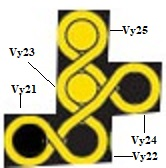
\includegraphics[width=0.3\textwidth]{figs/example.jpg}
    \caption{Name rules for yellow2}
    \label{fig:namerules}
\end{figure}
\subsection{Domains}
\begin{figure}[htbp]
\centering
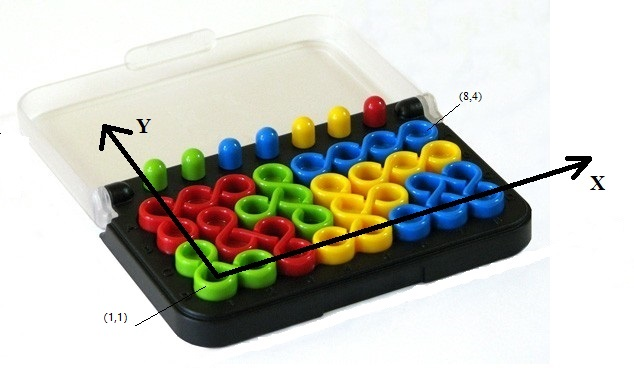
\includegraphics[width=0.8\textwidth]{figs/IQtwistboard.jpg}
\caption{The coordinate system for IQ Twist, revised from~\cite{r22}}
    \label{fig:coordinate}
\end{figure}
For the board, Figure~\ref{fig:coordinate} shows that the 2D coordinate system is used to represent the positions. In our model, all positions are represented as tuples and the elements in the tuples are int. In addition, each tuple contains 2 int. The left and bottom position as $(1,1)$ and the right and top as $(8,4)$. So, all placements will be between them. Considering a position $(x_{0},y_{0})$, we get
\begin{equation}
\begin{aligned}
&0<x_{0} \leq 8,\\
&0<y_{0} \leq 4.
\end{aligned}
\end{equation}
The placements for each unit of pieces must on the board, therefore, we get
\begin{equation}
\forall  v \in \VUnits \hspace{1ex},\hspace{1ex} D(v)=\{(i,j) \in \mathbb{Z} \times \mathbb{Z}	\mid  0<i \leq 8 \hspace{1ex} , \hspace{1ex} 0<j \leq 4\}.\\
\end{equation}
The pegs are special because they can be put in any places on the board or not on the board. So, the domain of pegs is
\begin{equation}
\forall  v \in \VPegs \hspace{1ex},\hspace{1ex} D(v)=\{(0,0)\} \hspace{1ex} \cup \hspace{1ex}\{(i,j) \in \mathbb{Z} \times \mathbb{Z}\mid  0<i \leq 8 \hspace{1ex} , \hspace{1ex} 0<j \leq 4\}.
\end{equation}
\subsection{2D Rotation Matrix}
\label{section:2Drotationmatrix}
To clarify how to obtain all configurations for each piece. I'd like to introduce 2D rotation matrix. 
\\In Figure~\ref{fig:explanation2D}, the unit which is corresponding to the first variable $V_{y21}$ will be considered as a point $(x_{0},y_{0})$. If we assign (0,0) to $(x_{0},y_{0})$, the $V_{y21}$, $V_{y22}$, $V_{y23}$, $V_{y24}$ and $V_{y25}$ can be respectively represented as $(0,0)$, $(1,0)$, $(1,1)$, $(2,1)$ and $(1,2)$, which indicate that all other variables are connection with the first variables. For example, there are relationships
\begin{equation}
\begin{aligned}
&x_{V_{y21}}+1=x_{V_{y22}},\\
&y_{V_{y21}}=y_{V_{y22}},
\end{aligned}
\end{equation}
between $V_{y21}$ and $V_{y22}$.
\begin{figure}[htbp]
\centering
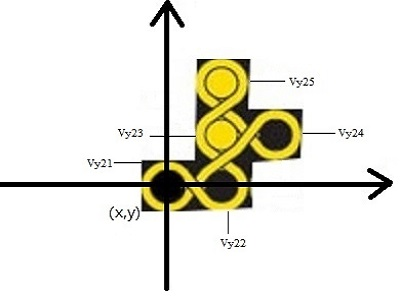
\includegraphics[width=0.5\textwidth]{figs/explanation2D.jpg}
\caption{The explanation of 2D rotation}
    \label{fig:explanation2D}
\end{figure}
Therefore, all other placements can be obtained from the initial state of the piece by rotations around the unit of piece $V_{y21}$.\\
Tobias and Krantz \cite{r9} mention that 2D rotation by an angle $\theta$ around the origin of coordinate can be described as a matrix
\begin{equation}
R(\theta)=\begin{bmatrix}
\cos\theta & -\sin\theta\\
\sin\theta & \cos\theta\\
\end{bmatrix}.
\end{equation}
If the initial position is (x,y), we can get the position after the rotation by
\begin{equation}
\label{equation:rotation}
\begin{bmatrix}
x'\\
y'\\
\end{bmatrix}
=\begin{bmatrix}
\cos\theta & -\sin\theta\\
\sin\theta & \cos\theta\\
\end{bmatrix}
\begin{bmatrix}
x\\
y\\
\end{bmatrix},
\end{equation}
which implies that 
\begin{equation}
\label{equation:formula1}
\begin{aligned}
&x'=x\cos\theta-y\sin\theta,\\
&y'=x\sin\theta+y\cos\theta.
\end{aligned}
\end{equation}
Therefore, if we assign 0, 90, 180 and 270 degrees to $\theta$, we get four configurations:
\begin{itemize}
  \item $x'=x\cos0^{\circ} - y\sin0^{\circ}\hspace{20pt},y'=x\sin0^{\circ} + y\cos0^{\circ}\hspace{24pt}\implies x'=x\hspace{10pt}, y'=y$
  \item $x'=x\cos90^{\circ} - y\sin90^{\circ}\hspace{10pt},y'=x\sin90^{\circ} + y\cos90^{\circ}\hspace{12pt}\implies x'=-y, y'=x$
  \item $x'=x\cos180^{\circ} - y\sin180^{\circ}, y'=x\sin180^{\circ} + y\cos180^{\circ} \implies x'=-x, y'=-y$
  \item $x'=x\cos270^{\circ} - y\sin270^{\circ}, y'=x\sin270^{\circ} + y\cos270^{\circ} \implies x'=y\hspace{10pt},y'=-x$
  \label{rotation4}
\end{itemize}
In IQ Twist, there exists a mirroring operation which corresponds to flpping a piece, if a unit of piece flip over around the y-axis, we get  (-x,y) from (x,y). Similarly, all the four configurations flip over around the y-axis. We get four more configurations: 
\begin{itemize}
  \item  $x'=x\hspace{10pt}, y'=y\hspace{10pt}$    flip over around the y-axis $\implies x''=-x\hspace{8pt},y''=y$
  \item  $x'=-y, y'=x\hspace{10pt}$                flip over around the y-axis $\implies x''=y,y''=x$
  \item  $x'=-x, y'=-y$               flip over around the y-axis $\implies x''=x, y''=-y$
  \item  $x'=y\hspace{10pt},y'=-x$    flip over around the y-axis $\implies x''=-y\hspace{8pt}, y''=-x$
  \label{mirrorrotate4}
\end{itemize}
Therefore, there should be a total of eight configurations for each unit of pieces. Similarly, for all units of piece in Figure~\ref{fig:explanation2D}, if we assign $(0,0)$ to $(x_{0},y_{0})$, the process of rotation for each other unit of the piece can be represented by Equation~\ref{equation:rotation}. Accordingly, we get eight possible configurations
\begin{itemize}
 \item $V_{y21}=(0,0)$, $V_{y22}=(1,0)$, $V_{y23}=(1,1)$, $V_{y24}=(2,1)$, $V_{y25}=(1,2)$,
 \item $V_{y21}=(0,0)$, $V_{y22}=(0,1)$, $V_{y23}=(-1,1)$, $V_{y24}=(-1,2)$, $V_{y25}=(-2,1)$,
 \item $V_{y21}=(0,0)$, $V_{y22}=(-1,0)$, $V_{y23}=(-1,-1)$, $V_{y24}=(-2,-1)$, $V_{y25}=(-1,-2)$,
 \item $V_{y21}=(0,0)$, $V_{y22}=(0,-1)$, $V_{y23}=(1,-1)$, $V_{y24}=(1,-2)$, $V_{y25}=(2,-1)$,
 \item $V_{y21}=(0,0)$, $V_{y22}=(-1,0)$, $V_{y23}=(-1,1)$, $V_{y24}=(-2,1)$, $V_{y25}=(-1,2)$,
 \item $V_{y21}=(0,0)$, $V_{y22}=(0,1)$, $V_{y23}=(1,1)$, $V_{y24}=(1,2)$, $V_{y25}=(2,1)$,
 \item $V_{y21}=(0,0)$, $V_{y22}=(1,0)$, $V_{y23}=(1,-1)$, $V_{y24}=(2,-1)$, $V_{y25}=(1,-2)$,
 \item $V_{y21}=(0,0)$, $V_{y22}=(-1,0)$, $V_{y23}=(-1,-1)$, $V_{y24}=(-2,-1)$, $V_{y25}=(-1,-2)$.
\end{itemize}
In our case, the piece can be moved as long as all units of piece on the board. Both the $x_{0}$ and $y_{0}$ can be variables, hence, we get the general forms
\begin{itemize}
 \item $V_{y21}=(x_{0},y_{0})$, $V_{y22}=(x_{0}+1,y_{0})$, $V_{y23}=(x_{0}+1,y_{0}+1)$, $V_{y24}=(x_{0}+2,y_{0}+1)$, $V_{y25}=(x_{0}+1,y_{0}+2)$,
 \item $V_{y21}=(x_{0},y_{0})$, $V_{y22}=(x_{0},y_{0}+1)$, $V_{y23}=(x_{0}-1,y_{0}+1)$, $V_{y24}=(x_{0}-1,y_{0}+2)$, $V_{y25}=(x_{0}-2,y_{0}+1)$,
 \item $V_{y21}=(x_{0},y_{0})$, $V_{y22}=(x_{0}-1,y_{0})$, $V_{y23}=(x_{0}-1,y_{0}-1)$, $V_{y24}=(x_{0}-2,y_{0}-1)$, $V_{y25}=(x_{0}-1,y_{0}-2)$,
 \item $V_{y21}=(x_{0},y_{0})$, $V_{y22}=(x_{0},y_{0}-1)$, $V_{y23}=(x_{0}+1,y_{0}-1)$, $V_{y24}=(x_{0}+1,y_{0}-2)$, $V_{y25}=(x_{0}+2,y_{0}-1)$,
 \item $V_{y21}=(x_{0},y_{0})$, $V_{y22}=(x_{0}-1,y_{0})$, $V_{y23}=(x_{0}-1,y_{0}+1)$, $V_{y24}=(x_{0}-2,y_{0}+1)$, $V_{y25}=(x_{0}-1,y_{0}+2)$,
 \item $V_{y21}=(x_{0},y_{0})$, $V_{y22}=(x_{0},y_{0}+1)$, $V_{y23}=(x_{0}+1,y_{0}+1)$, $V_{y24}=(x_{0}+1,y_{0}+2)$, $V_{y25}=(x_{0}+2,y_{0}+1)$,
 \item $V_{y21}=(x_{0},y_{0})$, $V_{y22}=(x_{0}+1,y_{0})$, $V_{y23}=(x_{0}+1,y_{0}-1)$, $V_{y24}=(x_{0}+2,y_{0}-1)$, $V_{y25}=(x_{0}+1,y_{0}-2)$,
 \item $V_{y21}=(x_{0},y_{0})$, $V_{y22}=(x_{0}-1,y_{0})$, $V_{y23}=(x_{0}-1,y_{0}-1)$, $V_{y24}=(x_{0}-2,y_{0}-1)$, $V_{y25}=(x_{0}-1,y_{0}-2)$.
\end{itemize}
\subsection{Constrains}
Firstly, there should be no 2 different unit variables contain the same value
\begin{equation}
\begin{aligned}
&\forall V_{m},V_{n} \in \VUnits,V_{m} \neq V_{n},\\
&\Constraints{m}{n}=\{((x_{1},y_{1}),(x_{2},y_{2}))\in \Domain{m} \times \Domain{n}\mid x_{1} \neq x_{2}   \hspace{1ex} or \hspace{1ex}  y_{1} \neq y_{2}\}.
\end{aligned}
\end{equation}
Similarly, there should be no 2 different reg variables contain the same value except both of them are not on the board
\begin{equation}
\begin{aligned}
&\forall V_{m},V_{n}\in \VPegs, V_{m} \neq V_{n},\\
&\Constraints{m}{n}=\{((x_{1},y_{1}),(x_{2},y_{2}))\in \Domain{m}\times \Domain{n}\mid x_{1} \neq x_{2}   \hspace{1ex} or \hspace{1ex}  y_{1} \neq y_{2}\}\hspace{1pt}\cup \\
&\{((0,0),(0,0))\}.
\end{aligned}
\end{equation}
As is mentioned in Chapter~\ref{section:2Drotationmatrix}, there should be eight configurations for general pieces. Figure~\ref{fig:Exampleof8} shows the eight configurations for yellow2. Hence,
\begin{figure}[htbp]
\centering
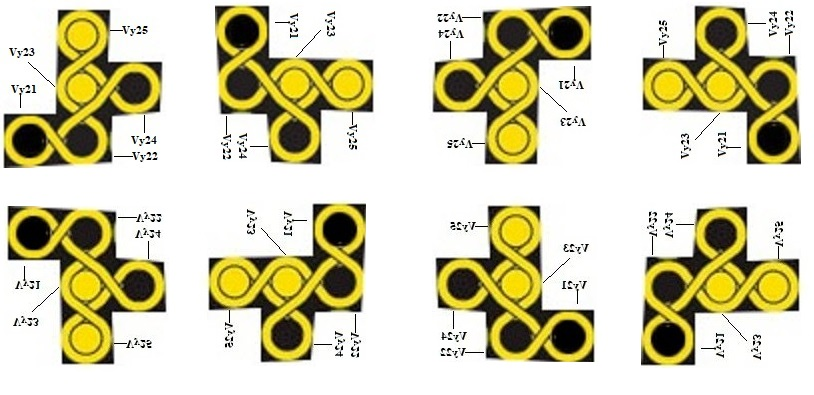
\includegraphics[width =\textwidth]{figs/domainexplain.jpg}
    \caption{Example of 8 configurations}
    \label{fig:Exampleof8}
\end{figure}
\begin{equation}
\begin{aligned}
\Cons{y21}{y22}{y23}{y24}{y25}=\{&((x_{1},y_{1}),(x_{2},y_{2}),(x_{3},y_{3}),(x_{4},y_{4}),(x_{5},y_{5}))\in \\
&\Domain {y21} \times \Domain{y22}\times \Domain{y23}\times \Domain{y24}\times \Domain{y25} \mid\\
&(x_{2} = x_{1} + 1,\hspace{1ex}y_{2} = y_{1},\hspace{1ex}x_{3} = x_{1}+1,\hspace{1ex}y_{3} = y_{1}+1,
\\&x_{4} = x_{1}+2,\hspace{1ex}y_{4} = y_{1}+1,\hspace{1ex}x_{5} = x_{1}+1,\hspace{1ex}y_{5} = y_{1}+2)\hspace{1ex} or \\
&(x_{2} = x_{1} ,\hspace{1ex}y_{2} = y_{1}+1,\hspace{1ex}x_{3} = x_{1}-1,\hspace{1ex}y_{3} = y_{1}+1,
\\&x_{4} = x_{1}-1,\hspace{1ex}y_{4} = y_{1}+2,\hspace{1ex}x_{5} = x_{1}-2,\hspace{1ex}y_{5} = y_{1}+1)\hspace{1ex} or \\
&(x_{2} = x_{1}-1 ,\hspace{1ex}y_{2} = y_{1},\hspace{1ex}x_{3} = x_{1}-1,\hspace{1ex}y_{3} = y_{1}-1,
\\&x_{4} = x_{1}-2,\hspace{1ex}y_{4} = y_{1}-1,\hspace{1ex}x_{5} = x_{1}-1,\hspace{1ex}y_{5} = y_{1}-2)\hspace{1ex} or \\
&(x_{2} = x_{1} ,\hspace{1ex}y_{2} = y_{1}-1,\hspace{1ex}x_{3} = x_{1}+1,\hspace{1ex}y_{3} = y_{1}-1,
\\&x_{4} = x_{1}+1,\hspace{1ex}y_{4} = y_{1}-2,\hspace{1ex}x_{5} = x_{1}+2,\hspace{1ex}y_{5} = y_{1}-1)\hspace{1ex} or \\
&(x_{2} = x_{1}-1 ,\hspace{1ex}y_{2} = y_{1},\hspace{1ex}x_{3} = x_{1}-1,\hspace{1ex}y_{3} = y_{1}+1,
\\&x_{4} = x_{1}-2,\hspace{1ex}y_{4} = y_{1}+1,\hspace{1ex}x_{5} = x_{1}-1,\hspace{1ex}y_{5} = y_{1}+2)\hspace{1ex} or \\
&(x_{2} = x_{1} ,\hspace{1ex}y_{2} = y_{1}-1,\hspace{1ex}x_{3} = x_{1}-1,\hspace{1ex}y_{3} = y_{1}-1,
\\&x_{4} = x_{1}-1,\hspace{1ex}y_{4} = y_{1}-2,\hspace{1ex}x_{5} = x_{1}-2,\hspace{1ex}y_{5} = y_{1}-1)\hspace{1ex} or \\
&(x_{2} = x_{1}+1 ,\hspace{1ex}y_{2} = y_{1},\hspace{1ex}x_{3} = x_{1}+1,\hspace{1ex}y_{3} = y_{1}-1,
\\&x_{4} = x_{1}+2,\hspace{1ex}y_{4} = y_{1}-1,\hspace{1ex}x_{5} = x_{1}+1,\hspace{1ex}y_{5} = y_{1}-2)\hspace{1ex} or \\
&(x_{2} = x_{1} ,\hspace{1ex}y_{2} = y_{1}+1,\hspace{1ex}x_{3} = x_{1}+1,\hspace{1ex}y_{3} = y_{1}+1,
\\&x_{4} = x_{1}+1,\hspace{1ex}y_{4} = y_{1}+2,\hspace{1ex}x_{5} = x_{1}+2,\hspace{1ex}y_{5} = y_{1}+1)\hspace{3ex}\}.
\end{aligned}
\end{equation}
Similarly, every piece can get the similar constraints (Appendix~\ref{appendix:2Dpieces}). Furthermore, for the pegs, unless they are not on the board, there must be a hollow unit of pieces which contains the same color with the pegs to match them. As an instance, for yellow peg1, there are 4 hollow units of yellow pieces. Therefore, we can obtain
\begin{equation}
\begin{aligned}  
\Constraint{py1} = &\{((x_{1},y_{1}),(x_{2},y_{2}))\in \Domain{py1} \times \Domain{y11}\mid x_{2} = x_{1} \hspace{1ex} , \hspace{1ex}  y_{2} = y_{1}\}\hspace{1ex} \cup  
\\&\{((x_{1},y_{1}),(x_{2},y_{2}))\in \Domain{py1} \times \Domain{y21}\mid x_{2} = x_{1} \hspace{1ex} , \hspace{1ex}  y_{2} = y_{1}\}\hspace{1ex} \cup 
\\&\{ ((x_{1},y_{1}),(x_{2},y_{2}))\in \Domain{py1} \times \Domain{y22}\mid x_{2} = x_{1} \hspace{1ex} , \hspace{1ex}  y_{2} = y_{1}\}\hspace{1ex}\cup 
\\& \{((x_{1},y_{1}),(x_{2},y_{2}))\in \Domain{py1} \times \Domain{y24}\mid x_{2} = x_{1} \hspace{1ex} , \hspace{1ex}  y_{2} = y_{1}\} \hspace{1ex}\cup
\\& \{(0,0)\}.
\end{aligned}
\end{equation}
Accordingly, every peg can get the similar constraints (Appendix~\ref{appendix:2Dpegs}).
\subsection{Implementation for IQ Twist}
\label{section:implementation1}
Based on the general CSP model, the specific model can be encoded in Minizinc. For example, 
\section{ZIG ZAG Puzzler}
Zig Zag Puzzler is a 3D puzzle game with 2 playing modes. Both games aim to place all pieces to full fill the game boards. In addition, for both of them, there are some pieces placed in advance to set the difficulty (Figure~\ref{fig:ZIG_ZAG_Puzzler_playing_modes}). Generally, the fewer pieces are placed in advance, the more difficult to solve the puzzler.
\begin{figure}[htbp]
    \centering
    \begin{subfigure}[b]{0.4\textwidth}
    
\includegraphics[width=\textwidth]{figs/zig_zag_mode1.jpg}
    \caption{One example of ZIG ZAG Puzzler playing mode1}
    \end{subfigure}
    \begin{subfigure}[b]{0.4\textwidth}
    
\includegraphics[width=\textwidth]{figs/zig_zag_mode2.jpg}
    \caption{One example of ZIG ZAG Puzzler playing mode2}
    \end{subfigure}
    \caption{ZIG ZAG Puzzler examples, adopted from~\cite{r23}}
    \label{fig:ZIG_ZAG_Puzzler_playing_modes}
\end{figure}
\\In this part, the designs of CSP models for Zig Zag Puzzler will be discussed. Generally, there are 2 playing modes, which uses the same pieces but different boards. On the condition of the two coordinates based on the same system which means both of them adopt right-handed coordinate or left-handed coordinate (Figure~\ref{figure:Cartesiancoordinate}), both of them can adopt the same variables and the same constraints but different domains. In our case, we adopt right-handed coordinate. 
\begin{figure}[htbp]
    \centering
    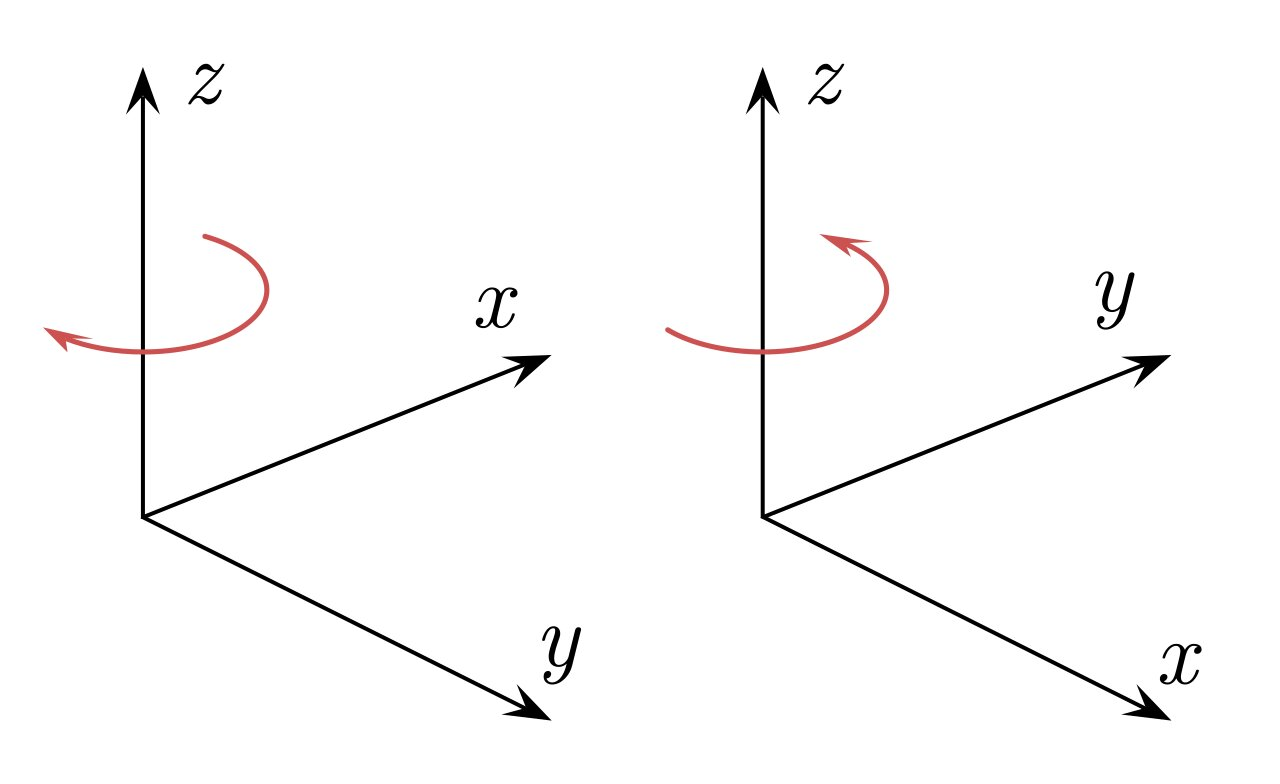
\includegraphics[width=0.8\textwidth]{figs/Cartesian_coordinate_system_handedness}
    \caption{Left-handed (left) coordinate and right-handed coordinate (right), adopted from~\cite{r20}}
    \label{figure:Cartesiancoordinate}
\end{figure}
\subsection{Variables}
Firstly, the initial state of each piece is defined in Figure~\ref{fig:all3Dinit}.
\label{section:3Dgame}
\begin{figure}[htbp]
\centering
\begin{subfigure}[b]{0.25\textwidth}
\centering
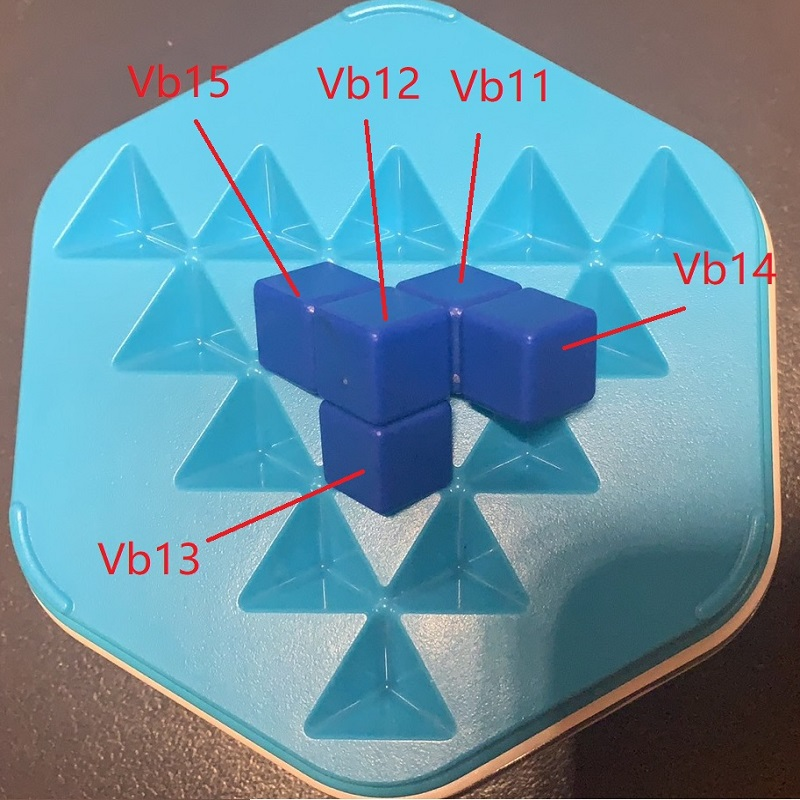
\includegraphics[width=\textwidth]{figs/3Dblue1.jpg}
\caption{The variable explanation of blue1}
  \label{fig:3Dblue1}
\end{subfigure}
\begin{subfigure}[b]{0.25\textwidth}
\centering
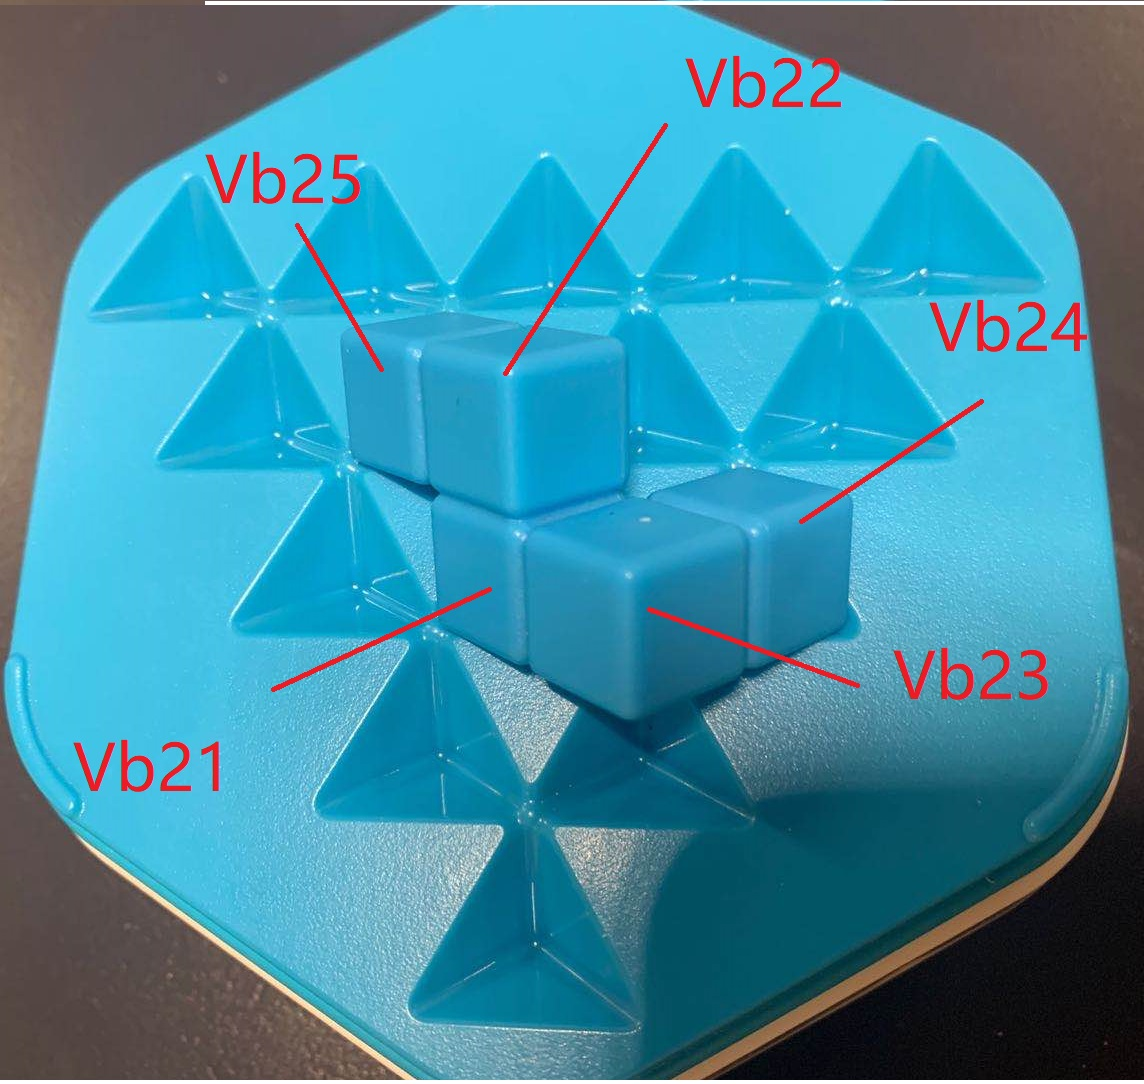
\includegraphics[width=\textwidth]{figs/3Dblue2.jpg}
\caption{The variable explanation of blue2}
  \label{fig:3Dblue2}
\end{subfigure}
\begin{subfigure}[b]{0.25\textwidth}
\centering
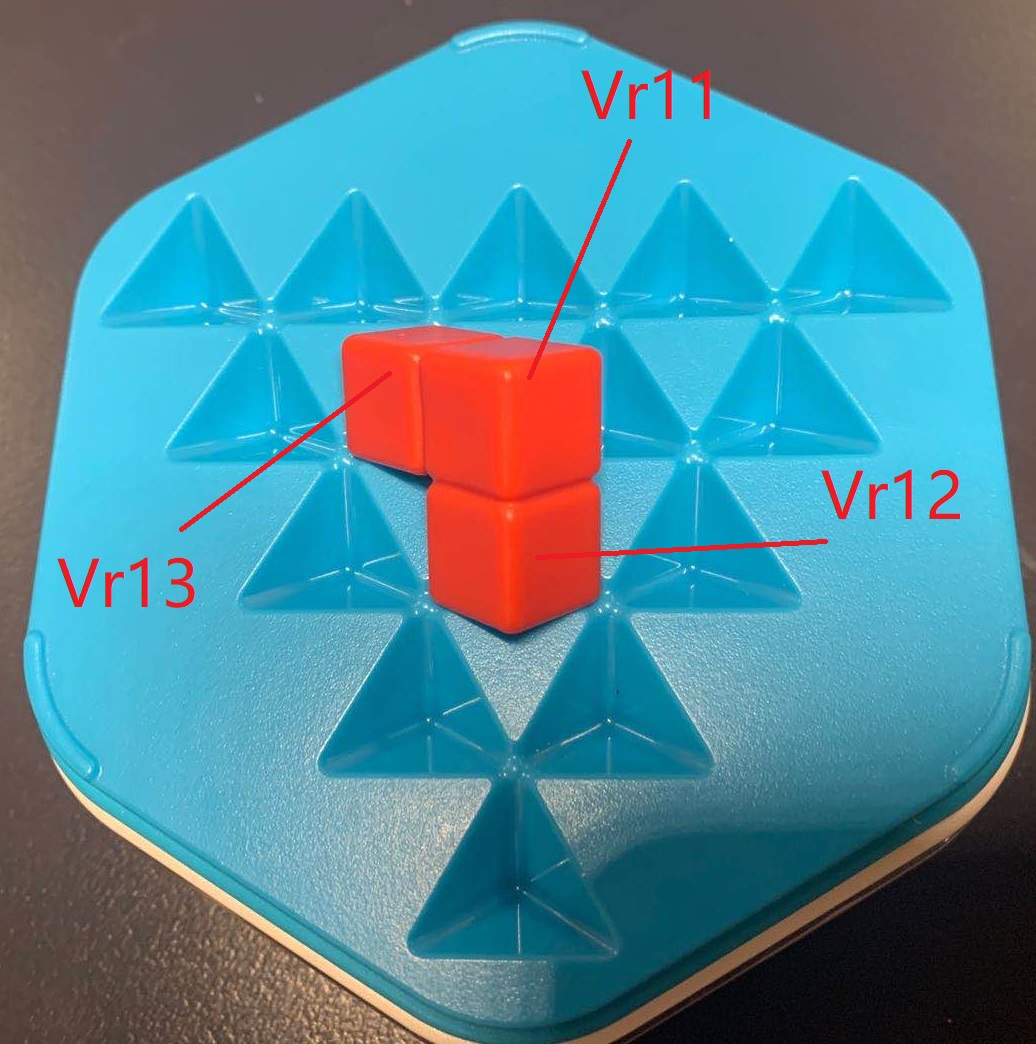
\includegraphics[width=\textwidth]{figs/3Dred1.jpg}
\caption{The variable explanation of red1}
  \label{fig:3Dred1}
\end{subfigure}
\begin{subfigure}[b]{0.25\textwidth}
\centering
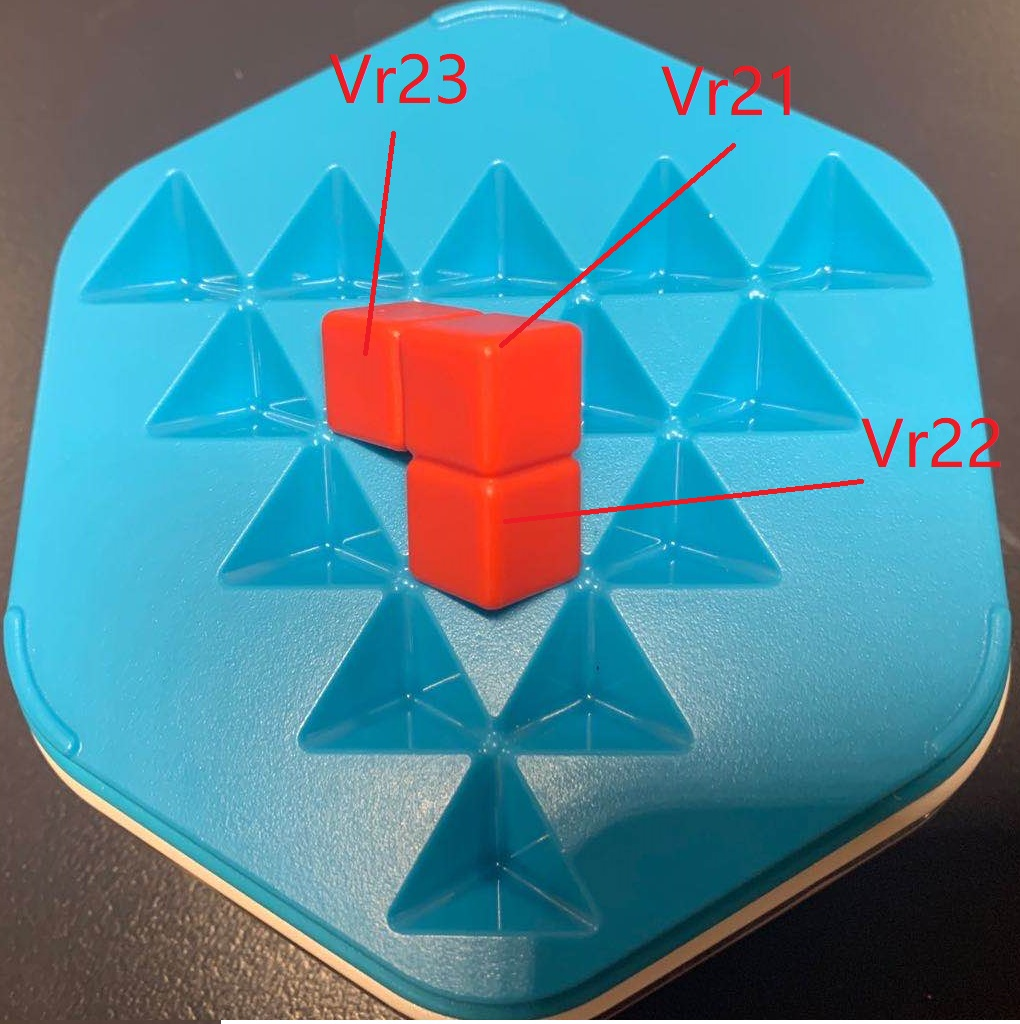
\includegraphics[width=\textwidth]{figs/3Dred2.jpg}
\caption{The variable explanation of red2}
  \label{fig:3Dred2}
\end{subfigure}
\begin{subfigure}[b]{0.25\textwidth}
\centering
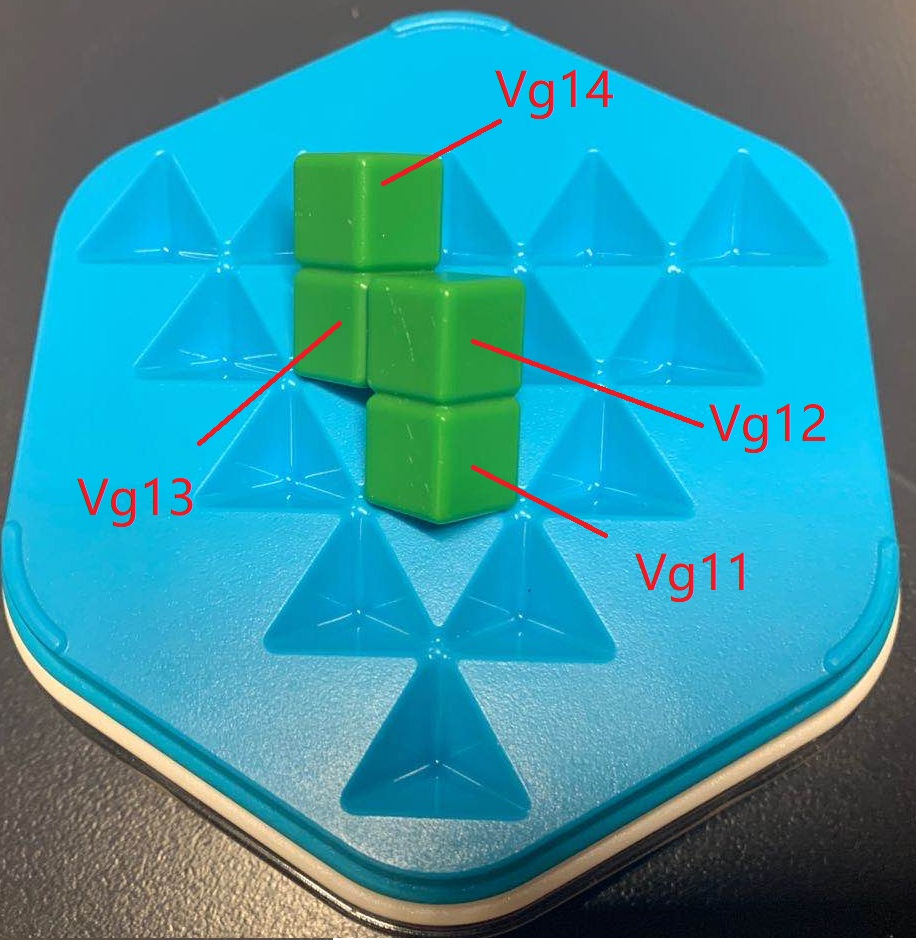
\includegraphics[width=\textwidth]{figs/3Dgreen1.jpg}
\caption{The variable explanation of green1}
  \label{fig:3Dgreen1}
\end{subfigure}
\begin{subfigure}[b]{0.25\textwidth}
\centering
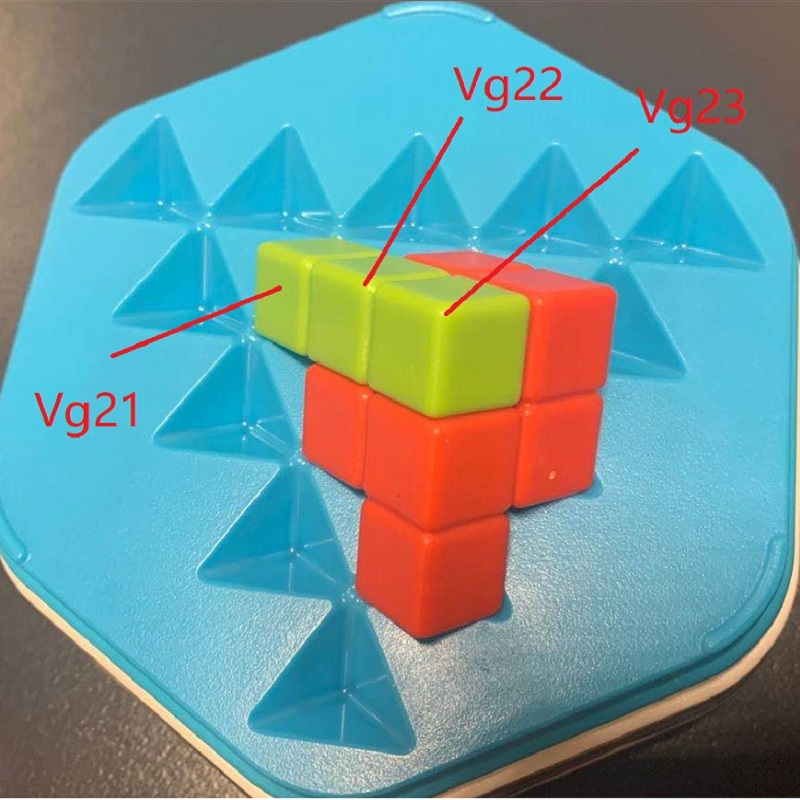
\includegraphics[width=\textwidth]{figs/3Dgreen2.jpg}
\caption{The variable explanation of green2}
  \label{fig:3Dgreen2}
\end{subfigure}
\begin{subfigure}[b]{0.25\textwidth}
\centering
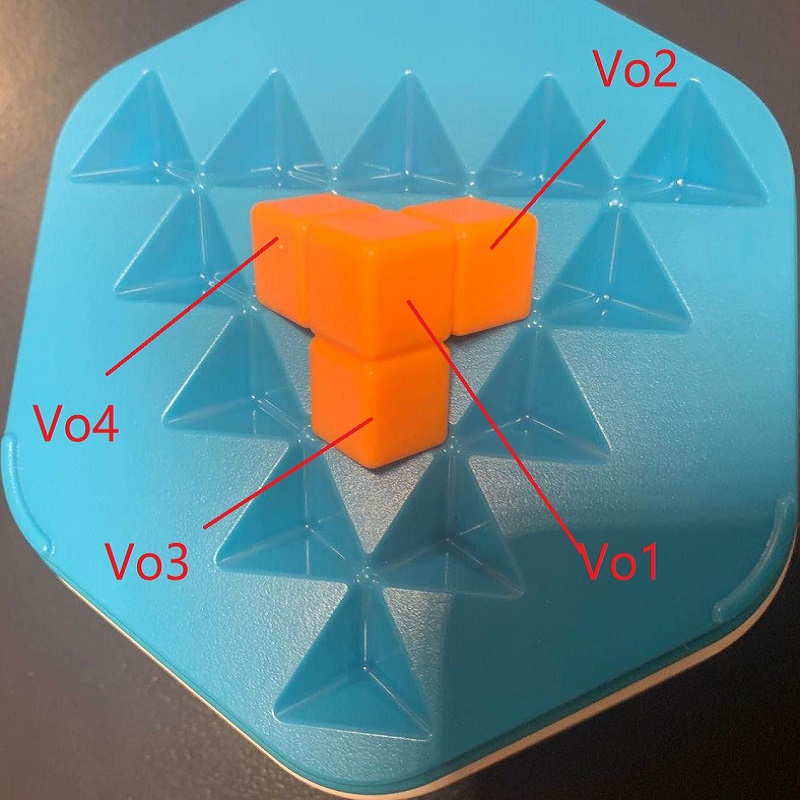
\includegraphics[width=\textwidth]{figs/3Dorange.jpg}
\caption{The variable explanation of orange}
  \label{fig:3Dorange}
\end{subfigure}
\begin{subfigure}[b]{0.25\textwidth}
\centering
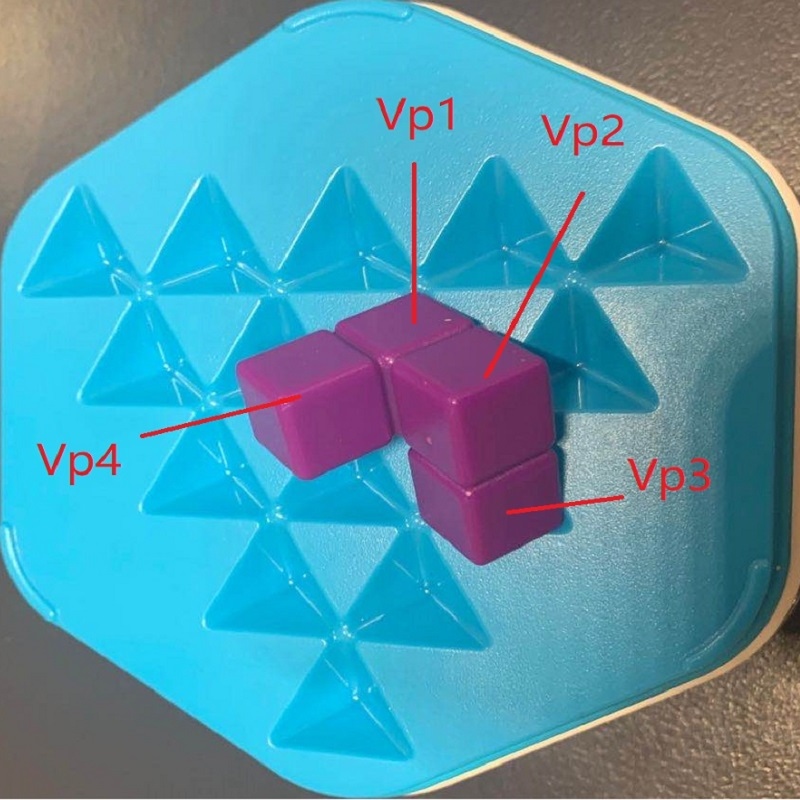
\includegraphics[width=\textwidth]{figs/3Dpurple.jpg}
\caption{The variable explanation of purple}
  \label{fig:3Dpurple}
\end{subfigure}
\begin{subfigure}[b]{0.25\textwidth}
\centering
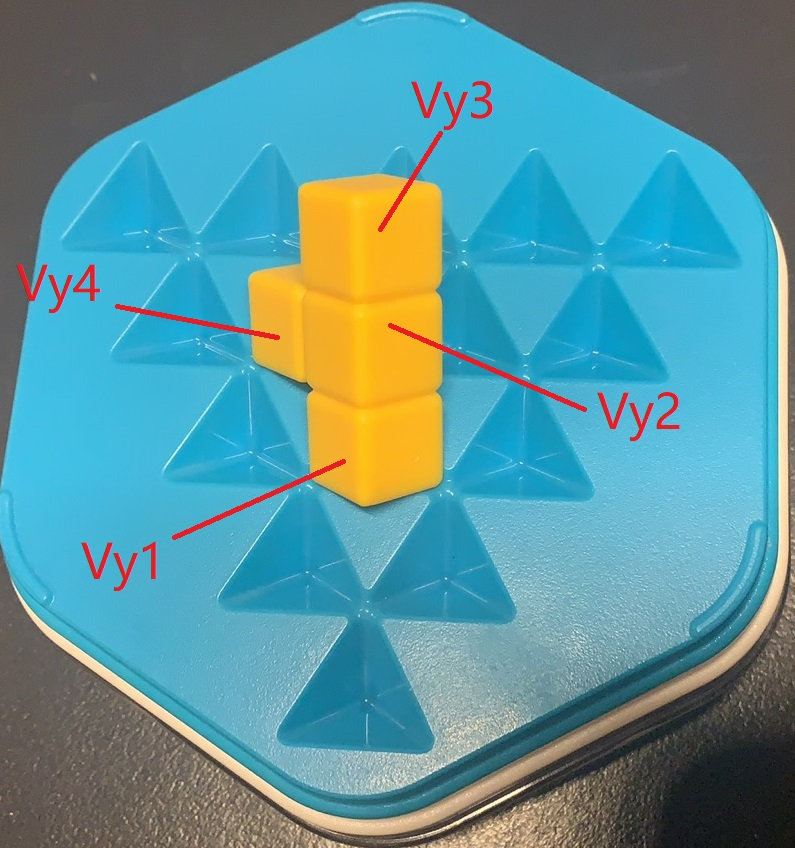
\includegraphics[width=\textwidth]{figs/3Dyellow.jpg}
\caption{The variable explanation of yellow}
  \label{fig:3Dyellow}
\end{subfigure}
\caption{Initial state of each piece}
  \label{fig:all3Dinit}
\end{figure}
It shows all the variables are corresponding to the specific units. Therefore, the variables can be defined as
\begin{equation}
\begin{aligned}
\VUnits=\{&V_{y1},V_{y2},V_{y3},V_{y4},\\&V_{b11},V_{b12},V_{b13},V_{b14},
V_{b15},\\&V_{b21},V_{b22},V_{b23},V_{b24},V_{b25},\\&V_{g11},V_{g12},V_{g13},V_{g14},\\&V_{g21},V_{g22},V_{g23},\\&V_{r11},
V_{r12},V_{r13},\\&V_{r21},V_{r22},V_{r23},\\&V_{o1},V_{o2},V_{o3},V_{o4},\\&V_{p1},V_{p2},V_{p3},V_{p4}\}.
\end{aligned}
\end{equation}
\subsection{Domains for Playing Mode 1 and 2}
\label{sec:3Ddomains}
Figure~\ref{fig:board1} and Figure~\ref{fig:board2} show how to create the coordinates for both modes to represent the positions of the boards. For of them, similar to IQ Twist, the positions are represented as tuples and the elements in tuples are int. But each tuple will contain 3 int. The unit of piece which is located in the origin of coordinate can be represented as $(1,1,1)$. So Considering one position $(x_{0},y_{0},z_{0})$.
\begin{figure}[htbp]
\centering
\begin{subfigure}[b]{.3\textwidth}
\centering
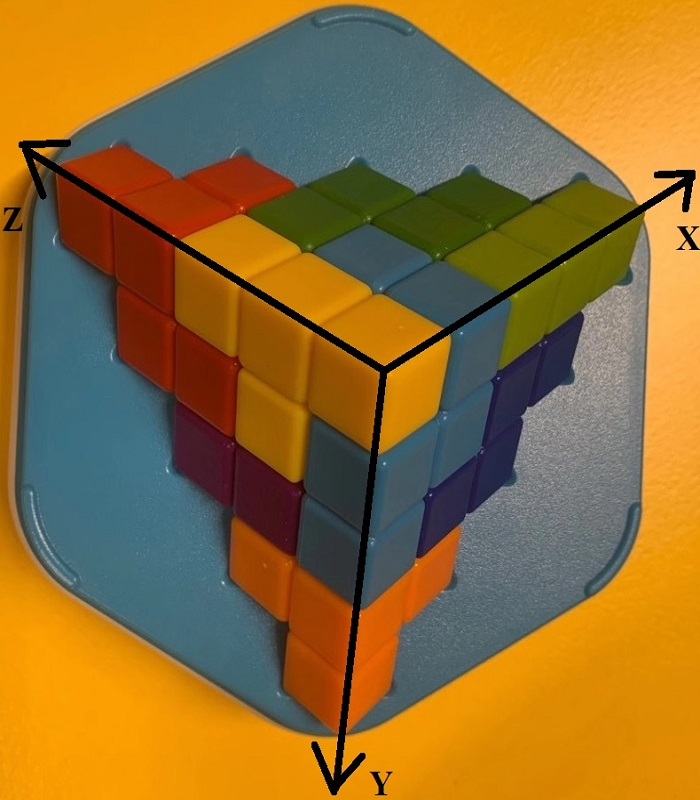
\includegraphics[width=\textwidth]{figs/ZIGZAGmodel1board.jpg}
\caption{}
\label{figure:mode1A}
\end{subfigure}
\begin{subfigure}[b]{.3\textwidth}
\centering
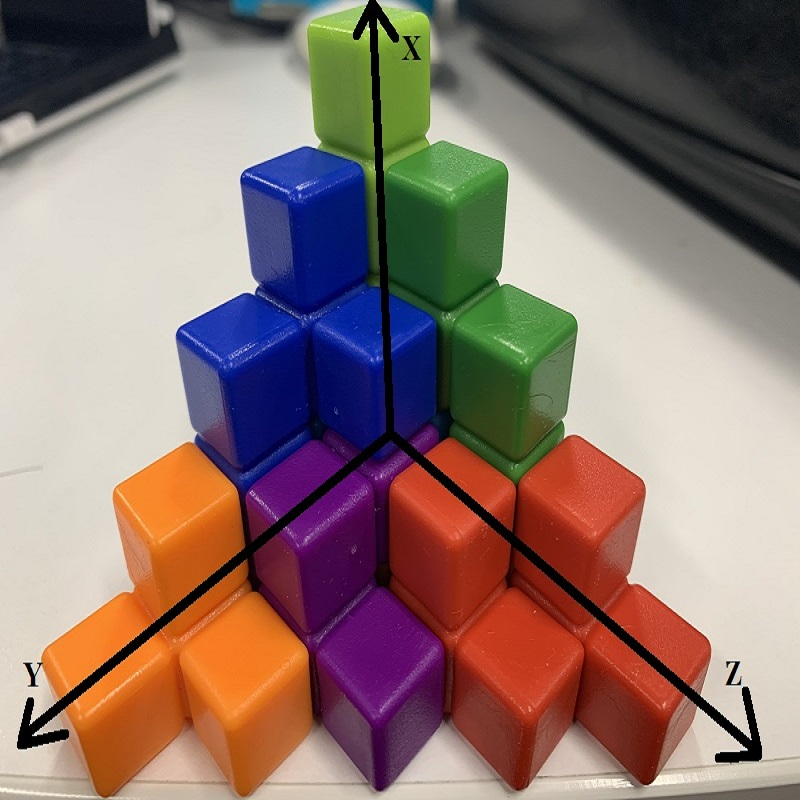
\includegraphics[width=\textwidth]{figs/3Dboard1.jpg}
\caption{}
\label{figure:mode1B}
\end{subfigure}
\caption{The board of ZIA ZAG Puzzler mode1}
  \label{fig:board1}
\end{figure}
\\For playing mode1, as is shown in Figure~\ref{fig:board1}, the maximum number for each axis is 5, hence,
\begin{equation}
\begin{aligned}
&0<x_{0}\leq5,\\
&0<y_{0}\leq5,\\
&0<z_{0}\leq5.
\end{aligned}
\end{equation}
If it is located in one of the 3 plane. Such as xy-plane $(x_{0},y_{0},1)$, it will satisfy
\begin{equation}
x_{0}+y_{0}\leq6.
\end{equation}
Accordingly, it will satisfy 
\begin{equation}
x_{0}+z_{0}\leq6
\end{equation}
in xz-plane and 
\begin{equation}
y_{0}+z_{0}\leq6
\end{equation}
in yz-plane. In addition, Figure~\ref{figure:mode1B} shows that all the units that are not in the 3 planes are close to one of the three planes, which means it's a unit of distance to one of the three plane. So we get
\begin{equation}
x_{0}+y_{0}+z_{0}\leq7.
\end{equation}
Because what we discussed above has included all positions, the domain of playing mode1 is
\begin{equation}
\begin{aligned}
&\forall \hspace{1ex} v \in \VUnits,\\
&D(v)=\{(x,y,z) \in \mathbb{Z} \times \mathbb{Z}	\times \mathbb{Z} \mid  0<x \leq 5, \hspace{1ex} 0<y \leq 5,\hspace{1ex} 0<z \leq 5,\\ &x+y\leq 6,\hspace{1ex} y+z\leq 6,\hspace{1ex}x+z\leq 6,\hspace{1ex}x+y+z\leq 7\}.
\end{aligned}
\end{equation}
\begin{figure}[htbp]
\centering
\begin{subfigure}[b]{.3\textwidth}
\centering
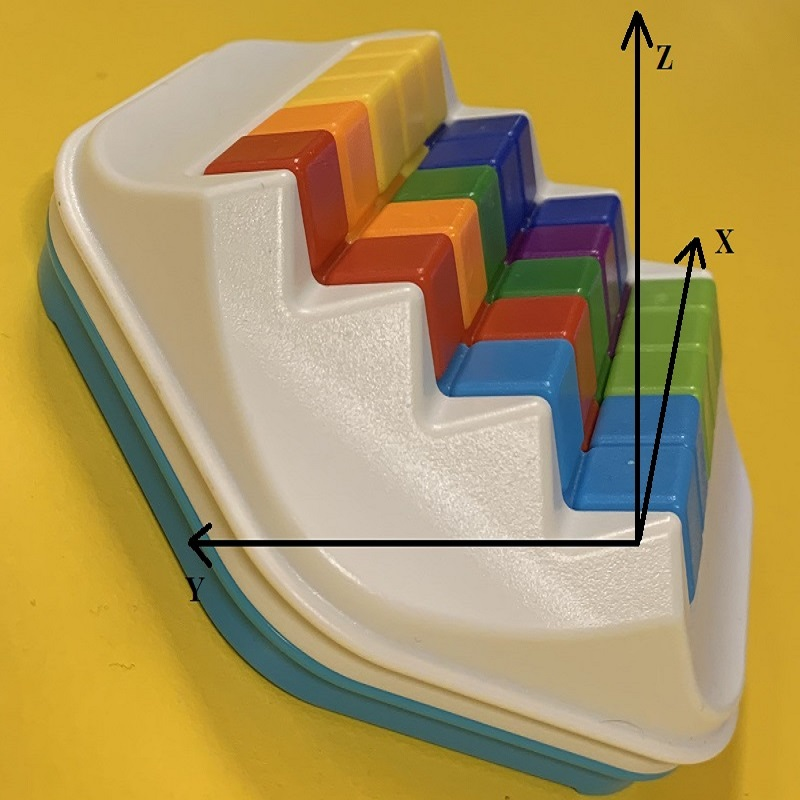
\includegraphics[width=\textwidth]{figs/ZIGZAGmodel2board.jpg}
\caption{}
\label{fig:board2A}
\end{subfigure}
\begin{subfigure}[b]{.3\textwidth}
\centering
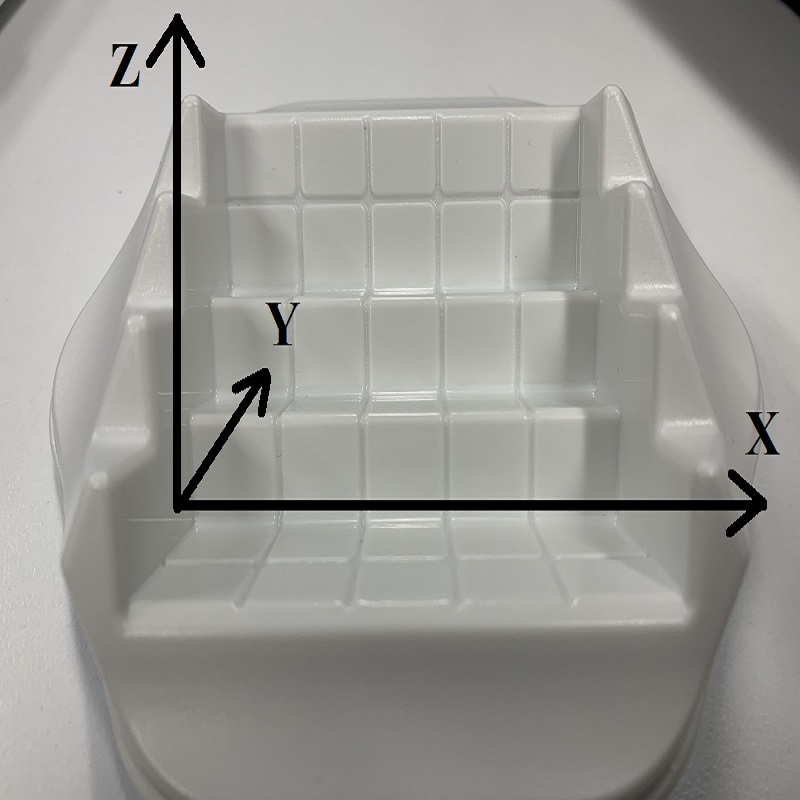
\includegraphics[width=\textwidth]{figs/3Dboard2.jpg}
\caption{}
\label{fig:board2B}
\end{subfigure}
\caption{The boards of ZIA ZAG Puzzler mode2}
  \label{fig:board2}
\end{figure}
For playing mode2, Figure~\ref{fig:board2} shows that the max number for both y-axis and z-axis are 4 and x-axis is 5, which can be represented as 
\begin{equation}
\begin{aligned}
&0<x_{0}\leq5,\\
&0<y_{0}\leq4,\\
&0<z_{0}\leq4.
\end{aligned}
\end{equation}
In addition, the board is similar to stairs, so we can get
\begin{equation}
y_{0}=z_{0}.
\end{equation}
Besides the part that is similar to stairs, the left space satisfy 
\begin{equation}
y_{0}=z_{0}+1,
\end{equation}
except when $z_{0}=4$.
Therefore, the domain of playing mode2 is
\begin{equation}
\begin{aligned}
&\forall v \in \VUnits,\\
&D(v)=\{(x,y,z) \in \mathbb{Z} \times \mathbb{Z}	\times \mathbb{Z} \mid  0<x \leq 5 , \hspace{1ex} 0<y \leq 4,\hspace{1ex} 0<z \leq 4,y=z\} \hspace{1ex}\cup\\
&\{(x,y,z) \in \mathbb{Z} \times \mathbb{Z}	\times \mathbb{Z} \mid  0<x \leq 5, \hspace{1ex} 0<y \leq 4,\hspace{1ex} 0<z \leq 3,y=z+1\}.
\end{aligned}
\end{equation}
\subsection{3D Rotation Matrix}
\label{section:3Drotationmatrix}
To clarify how to obtain all configurations for each piece.  I’d like to introduce 3D rotation matrix.
\begin{figure}[htbp]
\label{figure:3Dblue1}
\centering
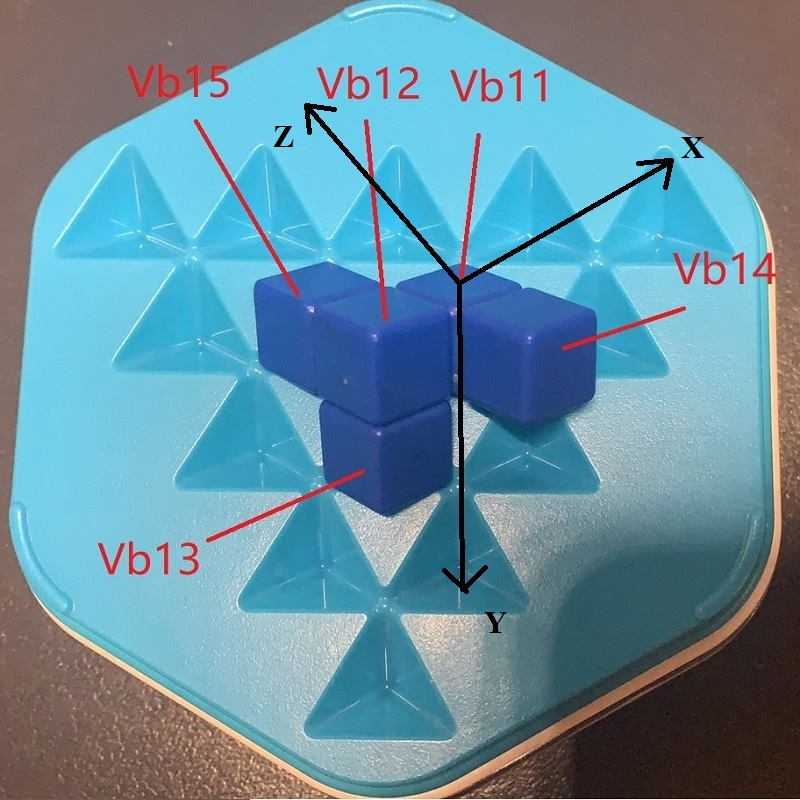
\includegraphics[width=0.3\textwidth]{figs/3Drotateexplain.jpg}
\caption{3Dblue1 initial state}
\label{fig:3Dblue1explanation}
\end{figure}
\\As is shown in Figure~\ref{fig:3Dblue1explanation}, the unit which is corresponding to the first variable $V_{b11}$ will be considered as a point $(x_{0},y_{0},z_{0})$. If we assign $(0,0,0)$ to $(x_{0},y_{0},z_{0})$, the $V_{b11}$, $V_{b12}$, $V_{b13}$, $V_{b14}$ and $V_{b15}$ are respectively represented as $(0,0,0)$, $(-1,0,0)$, $(-1,1,0)$, $(0,0,-1)$ and $(-1,0,1)$, which indicate that all other variables are connection with the first variables. For example, there are relationships
\begin{equation}
\begin{aligned}
&x_{V_{b11}}-1=x_{V_{b12}},\\
&y_{V_{b11}}=y_{V_{b12}},\\
&z_{V_{b11}}=z_{V_{b12}},
\end{aligned}
\end{equation}
between $V_{b11}$ and $V_{b12}$.
Similar to the pieces of IQ Twist, the basic idea for the pieces Zig Zag puzzler is all other units of pieces rotate around the first unit of the pieces.
\\Tobias and Krantz \cite{r9} indicate that 3D rotations can be separately represented by rotation around x-axis, y-axis, and z-axis 
\begin{equation}
\label{equation:3Dmatrix1}
\begin{aligned}
R_{x}(\theta_{1})=\begin{bmatrix}
1&          0&          0\\
0&\cos\theta_{1} & -\sin\theta_{1}\\
0&\sin\theta_{1} & \cos\theta_{1}\\
\end{bmatrix},
\\R_{y}(\theta_{2})=\begin{bmatrix}
  \cos\theta_{2}&          0&\sin\theta_{2}\\
           0&          1& 0\\
-\sin\theta_{2} &          0&\cos\theta_{2}\\
\end{bmatrix},
\\R_{z}(\theta_{3})=\begin{bmatrix}
\cos\theta_{3}&-\sin\theta_{3}&0\\
\sin\theta_{3}& \cos\theta_{3}&0\\
         0&          0&1\\
\end{bmatrix},
\end{aligned}
\end{equation}
where $R_{x}(\theta_{1})$ is corresponding to rotation around x-axis by $\theta_{1}$, $R_{y}(\theta_{2})$ is corresponding to the rotation around y-axis by $\theta_{2}$ and $R_{z}(\theta_{3})$ is corresponding to the rotation around z-axis by $\theta_{3}$. In addition, if a point rotate around x-axis by $\alpha$, y-axis by $\theta$ and z-axis by $\gamma$ at the same time, the combination of the three matrix in Equation~\ref{equation:3Dmatrix1} can be represented as
\begin{equation}
\label{equation:3Dmatrix2}
\begin{aligned}
&R=R_{z}(\alpha)R_{y}(\beta)R_{x}(\gamma)=\\
&\begin{bmatrix}
\cos\alpha\cos\beta&\cos\alpha\sin\beta\sin\gamma-\sin\alpha\cos\gamma&\cos\alpha\sin\beta\cos\gamma+\sin\alpha\sin\gamma\\
\sin\alpha\cos\beta&\sin\alpha\sin\beta\sin\gamma+\cos\alpha\cos\gamma&\sin\alpha\sin\beta\cos\gamma-\cos\alpha\sin\gamma\\
         -\sin\beta&                               \cos\beta\sin\gamma&\cos\beta\cos\gamma\\
\end{bmatrix}.
\end{aligned}
\end{equation}
In our case, we only consider 0, 90, 180 and 270 degrees rotations for each axis. If we separately consider each axis, there should be four configurations for each. As an example, according to $R_{x}(\theta_{1})$ in Equation~\ref{equation:3Dmatrix1}, when the point(x,y,z) rotate around x-axis by $\theta_{1}$, we get
\begin{equation}
\begin{bmatrix}
x'\\
y'\\
z'\\
\end{bmatrix}
=R_{x}(\theta_{1})
\begin{bmatrix}
x\\
y\\
z\\
\end{bmatrix}
\end{equation}, which implies
\begin{equation}
\label{equation:theta1}
\begin{aligned}
&x'=x,\\
&y'=y\cos\theta_{1}-z\sin\theta_{1},\\
&z'=y\sin\theta_{1}+z\cos\theta_{1}.
\end{aligned}
\end{equation}
Therefore, if we assign $0^{\circ}, 90^{\circ}, 180^{\circ}, 270^{\circ}$ to $\theta_{1}$ in Equation~\ref{equation:theta1}, we obtain $(x,y,z)$, $(x,-z,y)$, $(x,-y,-z)$ and $(x,z,-y)$.
Similarly, if a point rotates around the y-axis and the z-axis by $0^{\circ}$, $90^{\circ}$, $180^{\circ}$ and $270^{\circ}$, we can get 4 configurations each. Intuitively, the number of all possible configurations should be 64 because a point can rotate around x-axis by $\theta_{1}$ which is $0^{\circ}$, $90^{\circ}$, $180^{\circ}$ or $270^{\circ}$, rotate around y-axis by $\theta_{2}$ which is $0^{\circ}$, $90^{\circ}$, $180^{\circ}$ or $270^{\circ}$, and rotate around z-axis by $\theta_{3}$ which is $0^{\circ}$, $90^{\circ}$, $180^{\circ}$ or $270^{\circ}$. Therefore, the all possible situations should be the combination of $\theta_{1}$, $\theta_{2}$ and $\theta_{3}$, there should be a total of 64 configurations ($4\times 4 \times 4$). \\However, there are only 24 configurations because of the "singularities" of Euler angles set. Euler angles are three angles that used to represent the direction of rigid body in 3D space~\cite{r24}, which corresponds $\alpha$, $\beta$ and $\gamma$ in Equation~\ref{equation:3Dmatrix2}. Hughes~\cite{r19} highlights that "any set of Euler angles where the second rotation aligns the axes of the first and third rotations causes a singularity". The second rotation axis is y-axis, and the corresponding rotation angles is $\beta$. In addition, the geometric singularities only appear when $\beta=\pm90^{\circ}$ which is called "a repeated
axis sequence" as well as $\beta=0^{\circ}$ or $180^{\circ}$ which is called non-repeated axis
sequences~\cite{r17,r19}. How they cause singularities? Firstly, let us consider $\beta=\pm90^{\circ}$. If $\beta=90^{\circ}$, we get 
\begin{equation}
R_{\beta=90}=R_{z}(\alpha)R_{y}(90^{\circ})R_{x}(\gamma)=
\begin{bmatrix}
0&-\sin(\alpha-\gamma)&\cos(\alpha-\gamma)\\
0&\cos(\alpha-\gamma)&\sin(\alpha-\gamma)\\
         -1&                              0&0\\
\end{bmatrix}.
\end{equation}
And when $\beta=-90^{\circ}$, it can be seen as $\beta=270^{\circ}$ because of the periodicity, we can get 
\begin{equation}
R_{\beta=270}=R_{z}(\alpha)R_{y}(270^{\circ})R_{x}(\gamma)=
\begin{bmatrix}
0&-\sin(\alpha+\gamma)&-\cos(\alpha+\gamma)\\
0&\cos(\alpha+\gamma)&-\sin(\alpha+\gamma)\\
1&                               0&0
\end{bmatrix}.
\end{equation}
Based on the formula
\begin{equation}
\begin{bmatrix}
x'\\
y'\\
z'\\
\end{bmatrix}
=R
\begin{bmatrix}
x\\
y\\
z\\
\end{bmatrix},
\end{equation}
for $\beta=90^{\circ}$,
\begin{equation}
\label{equation:beta=90}
\begin{aligned}
&x'=-y\sin(\alpha-\gamma)-z\cos(\alpha-\gamma), \\
&y'=y\cos(\alpha-\gamma)+z\sin(\alpha-\gamma), \\
&z'=-x. 
\end{aligned}
\end{equation}
and for $\beta=270^{\circ}$, 
\begin{equation}
\label{equation:beta=270}
\begin{aligned}
&x'=-y\sin(\alpha+\gamma)-z\cos(\alpha+\gamma), \\
&y'=y\cos(\alpha+\gamma)-z\sin(\alpha+\gamma), \\
&z'=x.
\end{aligned}
\end{equation}
Because in our case, the domains of both $\alpha$ and $\gamma$ are $0^{\circ}$, $90^{\circ}$, $180^{\circ}$, $270^{\circ}$ and the period of the trigonometric function is $360^{\circ}$. For Equation~\ref{equation:beta=90}, the 4 configurations are $\alpha-\gamma$=$0^{\circ}$ or $90^{\circ}$ or $180^{\circ}$ or $270^{\circ}$. For Equation~\ref{equation:beta=270}, the 4 configurations are $\alpha+\gamma$=$0^{\circ}$ or $90^{\circ}$ or $180^{\circ}$ or $270^{\circ}$.
Therefore, these 2 groups of formulas represent that there are only 4 configurations for each of them. In other words, the separated $\alpha$ and $\gamma$ are meaningless. What we should consider is $\alpha-\gamma$ in Equation~\ref{equation:beta=90} and $\alpha+\gamma$ in Equation~\ref{equation:beta=270}. 
\\In Equation~\ref{equation:beta=90}, we assign 0,90,180 and 270 degrees to the $(\alpha-\gamma)$, we get four configurations:
\begin{itemize}
  \item  $x'=-y\sin(0^{\circ})-z\cos(0^{\circ}),\hspace{5pt} y'=y\cos(0^{\circ})+z\sin(0^{\circ}),\hspace{5pt} z'=-x \\\implies x'=-z,\hspace{5pt} y'=y,\hspace{5pt} z'=-x$
  \item  $x'=-y\sin(90^{\circ})-z\cos(90^{\circ}), \hspace{5pt} y'=y\cos(90^{\circ})+z\sin(90^{\circ}), \hspace{5pt} z'=-x\\\implies x'=-y,\hspace{5pt} y'=z,\hspace{5pt} z'=-x$
  \item  $x'=-y\sin(180^{\circ})-z\cos(180^{\circ}), \hspace{5pt} y'=y\cos(180^{\circ})+z\sin(180^{\circ}), \hspace{5pt} z'=-x\\\implies x'=z,\hspace{5pt} y'=-y,\hspace{5pt} z'=-x$
  \item  $x'=-y\sin(270^{\circ})-z\cos(270^{\circ}), \hspace{5pt} y'=y\cos(270^{\circ})+z\sin(270^{\circ}), \hspace{5pt} z'=-x\\\implies x'=y, \hspace{5pt}y'=-z,\hspace{5pt} z'=-x$
  \label{3Drotation24situations1}
\end{itemize}
In Equation~\ref{equation:beta=270}, we assign 0,90,180 and 270 degrees to the $(\alpha+\gamma)$, we get four configurations:
\begin{itemize}
  \item  $x'=-y\sin(0^{\circ})-z\cos(0^{\circ}),\hspace{5pt} y'=y\cos(0^{\circ})-z\sin(0^{\circ}),\hspace{5pt} z'=-x \\\implies x'=-z,\hspace{5pt} y'=y,\hspace{5pt} z'=x$
  \item  $x'=-y\sin(90^{\circ})-z\cos(90^{\circ}),\hspace{5pt} y'=y\cos(90^{\circ})-z\sin(90^{\circ}),\hspace{5pt} z'=-x\\\implies x'=-y,\hspace{5pt} y'=-z,\hspace{5pt} z'=x$
  \item  $x'=-y\sin(180^{\circ})-z\cos(180^{\circ}),\hspace{5pt} y'=y\cos(180^{\circ})-z\sin(180^{\circ}),\hspace{5pt} z'=-x\\\implies x'=z,\hspace{5pt} y'=-y,\hspace{5pt} z'=x$
  \item  $x'=-y\sin(270^{\circ})-z\cos(270^{\circ}),\hspace{5pt} y'=y\cos(270^{\circ})-z\sin(270^{\circ}),\hspace{5pt} z'=-x\\\implies x'=y, \hspace{5pt}y'=z,\hspace{5pt} z'=x$
  \label{3Drotation24situations2}
\end{itemize}
Then, we consider  $\beta=0^{\circ}$ and $\beta=180^{\circ}$. Based on (3.6), when $\beta=0^{\circ}$, we get
\begin{equation}
\label{equation:beta=0}
R=R_{z}(\alpha)R_{y}(0^{\circ})R_{x}(\gamma)=
\begin{bmatrix}
\cos\alpha&-\sin\alpha\cos\gamma&\sin\alpha\sin\gamma\\
\sin\alpha&\cos\alpha\cos\gamma&-\cos\alpha\sin\gamma\\
0&          \sin\gamma&\cos\gamma\\
\end{bmatrix}.
\end{equation}
When $\beta=180^{\circ}$, we get
\begin{equation}
\label{equation:beta=180}
R=R_{z}(\alpha)R_{y}(180^{\circ})R_{x}(\gamma)=
\begin{bmatrix}
-\cos\alpha&-\sin\alpha\cos\gamma&\sin\alpha\sin\gamma\\
-\sin\alpha&\cos\alpha\cos\gamma&-\cos\alpha\sin\gamma\\
0&                               -\sin\gamma&-\cos\gamma\\
\end{bmatrix}.
\end{equation}
In Equation~\ref{equation:beta=0}, we assign $\alpha=\alpha+180^{\circ}$ and $\gamma=\gamma+180^{\circ}$, then it change to
\begin{equation}
\label{equation:alphaandgamma}
\begin{aligned}
&R=R_{z}(\alpha+180^{\circ})R_{y}(180^{\circ})R_{x}(\gamma+180^{\circ})=\\
&\begin{bmatrix}
-\cos(\alpha+180^{\circ})&-\sin(\alpha+180^{\circ})\cos(\gamma+180^{\circ})&\sin(\alpha+180^{\circ})\sin(\gamma+180^{\circ})\\
-\sin(\alpha+180^{\circ})&\cos(\alpha+180^{\circ})\cos(\gamma+180^{\circ})&-\cos(\alpha+180^{\circ})\sin(\gamma+180^{\circ})\\
0&                               -\sin(\gamma+180^{\circ})&-\cos(\gamma+180^{\circ})
\end{bmatrix}\\
&=\begin{bmatrix}
\cos(\alpha)&-\sin(\alpha)\cos(\gamma)&\sin(\alpha)\sin(\gamma)\\
\sin(\alpha)&\cos(\alpha)\cos(\gamma)&-\cos(\alpha)\sin(\gamma)\\
0&                               \sin(\gamma)&\cos(\gamma)\\
\end{bmatrix}.
\end{aligned}
\end{equation}
Therefore, based on Equation~\ref{equation:beta=0} and Equation~\ref{equation:alphaandgamma},
\begin{equation}
R_{z}(\alpha)R_{y}(0^{\circ})R_{x}(\gamma)=R_{z}(\alpha+180^{\circ})R_{y}(180^{\circ})R_{x}(\gamma+180^{\circ}),
\end{equation}
which means that when $\beta=0^{\circ}$, regardless of the number of degrees of $\alpha$ and the number of degrees of $\gamma$, there are always corresponding $\alpha+180^{\circ}$, $\gamma+180^{\circ}$ when $\beta=180^{\circ}$. Even though the number of degrees of $\alpha+180^{\circ}$ or $\gamma+180^{\circ}$ may be more than $360^{\circ}$, it can always find a corresponding from $0^{\circ}$ to $360^{\circ}$ according to the periodicity of trigonometric function. For example, \begin{equation}
\begin{aligned}
&\circled{1}R_{z}(270^{\circ})Ry(0^{\circ})R_{x}(270^{\circ}) = R_{z}(450^{\circ})R_{y}(180^{\circ})R_{x}(450^{\circ})\\ 
&\circled{2}R_{z}(450^{\circ})Ry(180^{\circ})R_{x}(450^{\circ}) = R_{z}(90^{\circ})R_{y}(180^{\circ})R_{x}(90^{\circ})\\
&\circled{1},\circled{2}\implies R_{z}(270^{\circ})Ry(0^{\circ})R_{x}(270^{\circ})   = R_{z}(90^{\circ})R_{y}(180^{\circ})R_{x}(90^{\circ}).
\end{aligned}
\end{equation}
Hence, all combinations among $\beta=0^{\circ}$, $\theta=0^{\circ}$ or $90^{\circ}$ or $180^{\circ}$ or $270^{\circ}$ and $\gamma=0^{\circ}$ or $90^{\circ}$ or $180^{\circ}$ or $270^{\circ}$ can be obtained from one combination among $\beta=180^{\circ}$, $\theta=0^{\circ}$ or $90^{\circ}$ or $180^{\circ}$ or $270^{\circ}$ and $\gamma=0^{\circ}$ or $90^{\circ}$ or $180^{\circ}$ or $270^{\circ}$. So we only need to consider the all configurations when $\beta=0^{\circ}$ because the all configurations in $\beta=180^{\circ}$ are duplicates. For Equation~\ref{equation:beta=0}, we assign $\theta=0^{\circ},\gamma=0^{\circ}$; $\theta=0^{\circ},\gamma=90^{\circ}$;...;$\theta=270^{\circ},\gamma=180^{\circ}$; $\theta=270^{\circ},\gamma=270^{\circ}$. we get
\begin{itemize}
  \item  $x'=x$,   $y'=y$,    $z'=z$,
  \item  $x'=x$,   $y'=-z$,   $z'=y$, 
  \item  $x'=x$,   $y'=-y$,   $z'=-z$, 
  \item  $x'=x$,   $y'=z$,    $z'=-y$,
  \item  $x'=-y$,  $y'=x$,    $z'=z$,
  \item  $x'=z$,   $y'=x$,    $z'=y$,
  \item  $x'=y$,   $y'=x$,    $z'=-z$,
  \item  $x'=-z$,  $y'=x$,    $z'=-y$,
  \item  $x'=-x$,  $y'=-y$,   $z'=z$,
  \item  $x'=-x$,  $y'=z$,    $z'=y$,
  \item  $x'=-x$,  $y'=y$,    $z'=-z$,
  \item  $x'=-x$,  $y'=-z$,   $z'=-y$,
  \item  $x'=y$,   $y'=-x$,   $z'=z$,
  \item  $x'=-z$,  $y'=-x$,   $z'=y$,
  \item  $x'=-y$,  $y'=-x$,   $z'=-z$,
  \item  $x'=z$,   $y'=-x$,   $z'=-y$.
  \label{3Drotation24situations3}
\end{itemize}
There should be a total of 16 configurations (4$\times$4). Finally, consider the all configurations in $\beta=90^{\circ}$, $\beta=270^{\circ}$, $\beta=^{\circ}0$ and $\beta=180^{\circ}$. There should be a total of 4+4+16=24 configurations.
Therefore, if we assign $(0,0,0)$ to $Vb11$ in Figure~\ref{fig:3Dblue1explanation}, accordingly, we can get the initial state for $Vb12$, $Vb13$, $Vb14$ and $Vb15$, which corresponds as (-1,0,0), (-1,-1,0), (0,0,-1) and (-1,0,1). Based on the initial state, if all other units of piece rotate around Vb11, there should be 24 configurations. In our case, the piece can be moved as long as all units of piece on the board. Hence, on the condition of all units of piece on the board, we can assign variables $(x_{0},y_{0},z_{0})$ to $Vb11$, accordingly, we can get other units of piece's positions. Therefore, the constrains can be represented by the relationships between each other units of piece with the first unit of piece $Vb11$.
\subsection{Constraints}
According to chapter~\ref{section:3Drotationmatrix}, there are 24 rotation configurations. So we get
\begin{align*}
&\Cons{b11}{b12}{b13}{b14}{b15}=\{((x_{1},y_{1},z_{1}),(x_{2},y_{2},z_{2}),(x_{3},y_{3},z_{3}),(x_{4},y_{4},z_{4}),(x_{5},y_{5},z_{5}))\in \\
&\Domain {b11} \times \Domain{b12}\times \Domain{b13}\times \Domain{b14}\times \Domain{b15} \mid\\
&(x_{2}=x_{1}-1,\hspace{1ex} y_{2}=y_{1},\hspace{1ex} z_{2}=z_{1},\hspace{1ex} x_{3}=x_{1}-1,\hspace{1ex} y_{3}=y_{1}+1,\hspace{1ex} z_{3}=z_{1},\hspace{1ex} x_{4}=x_{1},\\
&\hspace{1ex} y_{4}=y_{1},\hspace{1ex} z_{4}=z_{1}-1,\hspace{1ex} x_{5}=x_{1}-1,\hspace{1ex} y_{5}=y_{1},\hspace{1ex} z_{5}=z_{1}+1)&or\\ 
&(x_{2}=x_{1},\hspace{1ex} y_{2}=y_{1}+1,\hspace{1ex} z_{2}=z_{1},\hspace{1ex} x_{3}=x_{1},\hspace{1ex} y_{3}=y_{1}+1,\hspace{1ex} z_{3}=z_{1}-1,\hspace{1ex} x_{4}=x_{1}-1,\\
&\hspace{1ex} y_{4}=y_{1},\hspace{1ex} z_{4}=z_{1},\hspace{1ex} x_{5}=x_{1}+1,\hspace{1ex} y_{5}=y_{1}+1,\hspace{1ex} z_{5}=z_{1})&or\\ 
&(x_{2}=x_{1},\hspace{1ex} y_{2}=y_{1}+1,\hspace{1ex} z_{2}=z_{1},\hspace{1ex} x_{3}=x_{1},\hspace{1ex} y_{3}=y_{1}+1,\hspace{1ex} z_{3}=z_{1}+1,\hspace{1ex} x_{4}=x_{1}+1,\\
&\hspace{1ex} y_{4}=y_{1},\hspace{1ex} z_{4}=z_{1},\hspace{1ex} x_{5}=x_{1}-1,\hspace{1ex} y_{5}=y_{1}+1,\hspace{1ex} z_{5}=z_{1})&or\\ 
&(x_{2}=x_{1},\hspace{1ex} y_{2}=y_{1},\hspace{1ex} z_{2}=z_{1}-1,\hspace{1ex} x_{3}=x_{1}-1,\hspace{1ex} y_{3}=y_{1},\hspace{1ex} z_{3}=z_{1}-1,\hspace{1ex} x_{4}=x_{1},\\
&\hspace{1ex} y_{4}=y_{1}+1,\hspace{1ex} z_{4}=z_{1},\hspace{1ex} x_{5}=x_{1},\hspace{1ex} y_{5}=y_{1}-1,\hspace{1ex} z_{5}=z_{1}-1)&or\\ 
&(x_{2}=x_{1}-1,\hspace{1ex} y_{2}=y_{1},\hspace{1ex} z_{2}=z_{1},\hspace{1ex} x_{3}=x_{1}-1,\hspace{1ex} y_{3}=y_{1}-1,\hspace{1ex} z_{3}=z_{1},\hspace{1ex} x_{4}=x_{1},\\
&\hspace{1ex} y_{4}=y_{1},\hspace{1ex} z_{4}=z_{1}+1,\hspace{1ex} x_{5}=x_{1}-1,\hspace{1ex} y_{5}=y_{1},\hspace{1ex} z_{5}=z_{1}-1)&or\\ 
&(x_{2}=x_{1}+1,\hspace{1ex} y_{2}=y_{1},\hspace{1ex} z_{2}=z_{1},\hspace{1ex} x_{3}=x_{1}+1,\hspace{1ex} y_{3}=y_{1}-1,\hspace{1ex} z_{3}=z_{1},\hspace{1ex} x_{4}=x_{1},\\
&\hspace{1ex} y_{4}=y_{1},\hspace{1ex} z_{4}=z_{1}-1,\hspace{1ex} x_{5}=x_{1}+1,\hspace{1ex} y_{5}=y_{1},\hspace{1ex} z_{5}=z_{1}+1)&or\\ 
&(x_{2}=x_{1},\hspace{1ex} y_{2}=y_{1}-1,\hspace{1ex} z_{2}=z_{1},\hspace{1ex} x_{3}=x_{1},\hspace{1ex} y_{3}=y_{1}-1,\hspace{1ex} z_{3}=z_{1}-1,\hspace{1ex} x_{4}=x_{1}+1,\\
&\hspace{1ex} y_{4}=y_{1},\hspace{1ex} z_{4}=z_{1},\hspace{1ex} x_{5}=x_{1}-1,\hspace{1ex} y_{5}=y_{1}-1,\hspace{1ex} z_{5}=z_{1})&or\\ 
&(x_{2}=x_{1},\hspace{1ex} y_{2}=y_{1}-1,\hspace{1ex} z_{2}=z_{1},\hspace{1ex} x_{3}=x_{1},\hspace{1ex} y_{3}=y_{1}-1,\hspace{1ex} z_{3}=z_{1}+1,\hspace{1ex} x_{4}=x_{1}-1,\\
&\hspace{1ex} y_{4}=y_{1},\hspace{1ex} z_{4}=z_{1},\hspace{1ex} x_{5}=x_{1}+1,\hspace{1ex} y_{5}=y_{1}-1,\hspace{1ex} z_{5}=z_{1})&or\\ 
&(x_{2}=x_{1},\hspace{1ex} y_{2}=y_{1}+1,\hspace{1ex} z_{2}=z_{1},\hspace{1ex} x_{3}=x_{1}+1,\hspace{1ex} y_{3}=y_{1}+1,\hspace{1ex} z_{3}=z_{1},\hspace{1ex} x_{4}=x_{1},\\
&\hspace{1ex} y_{4}=y_{1},\hspace{1ex} z_{4}=z_{1}-1,\hspace{1ex} x_{5}=x_{1},\hspace{1ex} y_{5}=y_{1}+1,\hspace{1ex} z_{5}=z_{1}+1)&or\\ 
&(x_{2}=x_{1},\hspace{1ex} y_{2}=y_{1},\hspace{1ex} z_{2}=z_{1}+1,\hspace{1ex} x_{3}=x_{1},\hspace{1ex} y_{3}=y_{1}-1,\hspace{1ex} z_{3}=z_{1}+1,\hspace{1ex} x_{4}=x_{1}+1,\\
&\hspace{1ex} y_{4}=y_{1},\hspace{1ex} z_{4}=z_{1},\hspace{1ex} x_{5}=x_{1}-1,\hspace{1ex} y_{5}=y_{1},\hspace{1ex} z_{5}=z_{1}+1)&or\\ 
&(x_{2}=x_{1},\hspace{1ex} y_{2}=y_{1},\hspace{1ex} z_{2}=z_{1}+1,\hspace{1ex} x_{3}=x_{1}+1,\hspace{1ex} y_{3}=y_{1},\hspace{1ex} z_{3}=z_{1}+1,\hspace{1ex} x_{4}=x_{1},\\
&\hspace{1ex} y_{4}=y_{1}+1,\hspace{1ex} z_{4}=z_{1},\hspace{1ex} x_{5}=x_{1},\hspace{1ex} y_{5}=y_{1}-1,\hspace{1ex} z_{5}=z_{1}+1)&or\\ 
&(x_{2}=x_{1},\hspace{1ex} y_{2}=y_{1},\hspace{1ex} z_{2}=z_{1}-1,\hspace{1ex} x_{3}=x_{1},\hspace{1ex} y_{3}=y_{1}+1,\hspace{1ex} z_{3}=z_{1}-1,\hspace{1ex} x_{4}=x_{1}+1,\\
&\hspace{1ex} y_{4}=y_{1},\hspace{1ex} z_{4}=z_{1},\hspace{1ex} x_{5}=x_{1}-1,\hspace{1ex} y_{5}=y_{1},\hspace{1ex} z_{5}=z_{1}-1)&or\\ 
&(x_{2}=x_{1},\hspace{1ex} y_{2}=y_{1}-1,\hspace{1ex} z_{2}=z_{1},\hspace{1ex} x_{3}=x_{1}-1,\hspace{1ex} y_{3}=y_{1}-1,\hspace{1ex} z_{3}=z_{1},\hspace{1ex} x_{4}=x_{1},\\
&\hspace{1ex} y_{4}=y_{1},\hspace{1ex} z_{4}=z_{1}-1,\hspace{1ex} x_{5}=x_{1},\hspace{1ex} y_{5}=y_{1}-1,\hspace{1ex} z_{5}=z_{1}+1)&or\\ 
&(x_{2}=x_{1}+1,\hspace{1ex} y_{2}=y_{1},\hspace{1ex} z_{2}=z_{1},\hspace{1ex} x_{3}=x_{1}+1,\hspace{1ex} y_{3}=y_{1},\hspace{1ex} z_{3}=z_{1}-1,\hspace{1ex} x_{4}=x_{1},\\
&\hspace{1ex} y_{4}=y_{1}+1,\hspace{1ex} z_{4}=z_{1},\hspace{1ex} x_{5}=x_{1}+1,\hspace{1ex} y_{5}=y_{1}-1,\hspace{1ex} z_{5}=z_{1})&or\\
&(x_{2}=x_{1}+1,\hspace{1ex} y_{2}=y_{1},\hspace{1ex} z_{2}=z_{1},\hspace{1ex} x_{3}=x_{1}+1,\hspace{1ex} y_{3}=y_{1}+1,\hspace{1ex} z_{3}=z_{1},\hspace{1ex} x_{4}=x_{1},\\
&\hspace{1ex} y_{4}=y_{1},\hspace{1ex} z_{4}=z_{1}+1,\hspace{1ex} x_{5}=x_{1}+1,\hspace{1ex} y_{5}=y_{1},\hspace{1ex} z_{5}=z_{1}-1)&or\\ 
&(x_{2}=x_{1},\hspace{1ex} y_{2}=y_{1},\hspace{1ex} z_{2}=z_{1}-1,\hspace{1ex} x_{3}=x_{1},\hspace{1ex} y_{3}=y_{1}-1,\hspace{1ex} z_{3}=z_{1}-1,\hspace{1ex} x_{4}=x_{1}-1,\\
&\hspace{1ex} y_{4}=y_{1},\hspace{1ex} z_{4}=z_{1},\hspace{1ex} x_{5}=x_{1}+1,\hspace{1ex} y_{5}=y_{1},\hspace{1ex} z_{5}=z_{1}-1)&or\\ 
&(x_{2}=x_{1},\hspace{1ex} y_{2}=y_{1},\hspace{1ex} z_{2}=z_{1}+1,\hspace{1ex} x_{3}=x_{1},\hspace{1ex} y_{3}=y_{1}+1,\hspace{1ex} z_{3}=z_{1}+1,\hspace{1ex} x_{4}=x_{1}-1,\\
&\hspace{1ex} y_{4}=y_{1},\hspace{1ex} z_{4}=z_{1},\hspace{1ex} x_{5}=x_{1}+1,\hspace{1ex} y_{5}=y_{1},\hspace{1ex} z_{5}=z_{1}+1)&or\\ 
&(x_{2}=x_{1},\hspace{1ex} y_{2}=y_{1},\hspace{1ex} z_{2}=z_{1}-1,\hspace{1ex} x_{3}=x_{1}+1,\hspace{1ex} y_{3}=y_{1},\hspace{1ex} z_{3}=z_{1}-1,\hspace{1ex} x_{4}=x_{1},\\
&\hspace{1ex} y_{4}=y_{1}-1,\hspace{1ex} z_{4}=z_{1},\hspace{1ex} x_{5}=x_{1},\hspace{1ex} y_{5}=y_{1}+1,\hspace{1ex} z_{5}=z_{1}-1)&or\\ 
&(x_{2}=x_{1},\hspace{1ex} y_{2}=y_{1}-1,\hspace{1ex} z_{2}=z_{1},\hspace{1ex} x_{3}=x_{1}+1,\hspace{1ex} y_{3}=y_{1}-1,\hspace{1ex} z_{3}=z_{1},\hspace{1ex} x_{4}=x_{1},\\
&\hspace{1ex} y_{4}=y_{1},\hspace{1ex} z_{4}=z_{1}+1,\hspace{1ex} x_{5}=x_{1},\hspace{1ex} y_{5}=y_{1}-1,\hspace{1ex} z_{5}=z_{1}-1)&or\\ 
&(x_{2}=x_{1},\hspace{1ex} y_{2}=y_{1}+1,\hspace{1ex} z_{2}=z_{1},\hspace{1ex} x_{3}=x_{1}-1,\hspace{1ex} y_{3}=y_{1}+1,\hspace{1ex} z_{3}=z_{1},\hspace{1ex} x_{4}=x_{1},\\
&\hspace{1ex} y_{4}=y_{1},\hspace{1ex} z_{4}=z_{1}+1,\hspace{1ex} x_{5}=x_{1},\hspace{1ex} y_{5}=y_{1}+1,\hspace{1ex} z_{5}=z_{1}-1)&or\\ 
&(x_{2}=x_{1}+1,\hspace{1ex} y_{2}=y_{1},\hspace{1ex} z_{2}=z_{1},\hspace{1ex} x_{3}=x_{1}+1,\hspace{1ex} y_{3}=y_{1},\hspace{1ex} z_{3}=z_{1}+1,\hspace{1ex} x_{4}=x_{1},\\
&\hspace{1ex} y_{4}=y_{1}-1,\hspace{1ex} z_{4}=z_{1},\hspace{1ex} x_{5}=x_{1}+1,\hspace{1ex} y_{5}=y_{1}+1,\hspace{1ex} z_{5}=z_{1})&or\\ 
&(x_{2}=x_{1}-1,\hspace{1ex} y_{2}=y_{1},\hspace{1ex} z_{2}=z_{1},\hspace{1ex} x_{3}=x_{1}-1,\hspace{1ex} y_{3}=y_{1},\hspace{1ex} z_{3}=z_{1}+1,\hspace{1ex} x_{4}=x_{1},\\
&\hspace{1ex} y_{4}=y_{1}+1,\hspace{1ex} z_{4}=z_{1},\hspace{1ex} x_{5}=x_{1}-1,\hspace{1ex} y_{5}=y_{1}-1,\hspace{1ex} z_{5}=z_{1})&or\\ 
&(x_{2}=x_{1},\hspace{1ex} y_{2}=y_{1},\hspace{1ex} z_{2}=z_{1}+1,\hspace{1ex} x_{3}=x_{1}-1,\hspace{1ex} y_{3}=y_{1},\hspace{1ex} z_{3}=z_{1}+1,\hspace{1ex} x_{4}=x_{1},\\
&\hspace{1ex} y_{4}=y_{1}-1,\hspace{1ex} z_{4}=z_{1},\hspace{1ex} x_{5}=x_{1},\hspace{1ex} y_{5}=y_{1}+1,\hspace{1ex} z_{5}=z_{1}+1)&or\\ 
&(x_{2}=x_{1}-1,\hspace{1ex} y_{2}=y_{1},\hspace{1ex} z_{2}=z_{1},\hspace{1ex} x_{3}=x_{1}-1,\hspace{1ex} y_{3}=y_{1},\hspace{1ex} z_{3}=z_{1}-1,\hspace{1ex} x_{4}=x_{1},\\
&\hspace{1ex} y_{4}=y_{1}-1,\hspace{1ex} z_{4}=z_{1},\hspace{1ex} x_{5}=x_{1}-1,\hspace{1ex} y_{5}=y_{1}+1,\hspace{1ex} z_{5}=z_{1})\}.
\end{align*}
Similarly, we can get the constraints for other pieces.
\subsection{Implementation}
\chapter{Evaluation}
\label{cha:evaluation}
\section{Experiment Environment}
\subsection{Compiler}
\label{section:compiler}
Minizinc IDE is a compiler which allows users to edit and run their models, which is developed by the University of Melbourne, Monash University, and Data61 Decision Sciences~\cite{r6}. It provides some built-in functions as well as optimization methods. In our models, the build-in algorithm that aims to achieve singleton arc consistent and the built-in Minizinc-to-Flatzinc translator have been applied. In addition, a wide range of solvers has been tested~\cite{r6}. In our case, because the CSPs can be considered as mixed-integer programming (MIP) problems too, there are some MIP solvers.
\begin{itemize}
    \item \emph{Choco}: A Java CSP solver, which supports many search strategies (DomWDeg, ABS, IBS, first-fail, etc.) and optimization processes (LNS, fast restart).
    \item \emph{Chuffed}: A C++ finite domain solver using lazy clause generation, which contains a nogood logbook to avoid plenty of duplicate calculation.
    \item \emph{Coin-bc}: A C++ based MIP solver, it adopts the branch and cut optimization.
    \item \emph{Gurobi}: A commercial solver supports MIP.
    \item \emph{Izplus}: Based on iZ-C constraint programming that is developed by NTT DATA SEKISUI SYSTEMS CORPORATION. It combines Randomized restarting, Local search, Variable reordering and nogood learning.
    \item \emph{Jacop}: A Java CSP solver.
    \item \emph{OR-Tools}: An open-source solver developed by google, it combines many optimization methods.
    \item \emph{PicatSAT}: A CSP solver based on picat which is a rule-based language. And it adopts log encoding~\cite{r8}.
    \item \emph{Yuck}: Based on Scala and combines local search with restarting, global constraints, and lexicographic cost functions.
\end{itemize}
\subsection{Software Platform and Hardware Platform}
\label{sec:softplat}
Most of the experiments are based on the Windows subsystem for Linux 2 (WSL2) \footnote{https://docs.microsoft.com/en-us/windows/wsl/about} which allows the developer to run a Linux environment on Windows 10. Only the experiments related to izplus based on docker. Docker is a lightweight virtual machine that applied container virtualization technology~\cite{r25}. Docker provides a Linux environment as well. Table~\ref{tab:Ubuntu} shows the version of WSL2.
\begin{table*}[htbp]
  \centering

  \caption{The version of Windows subsystem for Linux 2}
  
  \label{tab:Ubuntu}
  \input table/Ubuntuversion.tex
\end{table*}
Furthermore, as mentioned in Chapter~\ref{section:compiler}, there are nine solvers that have been applied in our experiment, Table~\ref{tab:solvers} indicates the version of each solver.
\begin{table}[htbp]
  \centering

  \caption{The deployed solvers and corresponding versions}
  
  \label{tab:solvers}
  	\begin{subtable}[b]{\textwidth}
  	\centering
  \input table/solver1.tex
    \end{subtable}\\
    	\begin{subtable}[b]{\textwidth}
  	\centering
  \input table/solver2.tex
  \end{subtable}\\
  \begin{subtable}[b]{\textwidth}
  \centering
  \input table/solver3.tex
  \end{subtable}
\end{table}
\\In addition, Table~\ref{tab:machines} introduces the configurations of the hardware platform.
\begin{table}[H]
  \centering

  \caption{Processor used in our evaluation}
  
  \label{tab:machines}
  \input table/machines.tex
\end{table}
\section{Results}
\label{sec:Result}
In this section, both the results of IQ Twist's experiments and the results of Zig Zag Puzzler's experiments will be discussed. Generally, all the problems in both games' booklets have been tested by the nine solvers that are mentioned in Table~\ref{tab:solvers}. For each game, there are five difficulties 'start', 'junior', 'expert', 'master' and 'wizard'. Each difficulty consists of some problems. The time limit for running each problem is 30 minutes, which is represented as 1800 seconds. If the solver can get the result in 1800 seconds, the time will be logged, otherwise, it will be treated as an unsolved problem, and the execution time will be logged as 1800 seconds. 
\\Above all, the discussions for the result will mainly include two parts, the coverage rates and the execution time of each solver. 
\\For the coverage rates, it can be calculated by 
\begin{equation}
\label{equation:coverage}
   C= N1/N2,
\end{equation}
where $C$ means the coverage rates, $N1$ means the number of solved problems and $N2$ means the number of total problems, in our case, the overall coverage and separated coverage that corresponds to different difficulties will be discussed.
\\And for the logged execution time, except for all the logged execution time points, the average execution time will be considered as well. It can be calculated by 
\begin{equation}
\label{equation:averagetime}
\overline{t}=\frac{\sum\limits_{i=1}^n t_{i}}{n},
\end{equation}
where $\overline{t}$ is the average execution time, $\sum\limits_{i=1}^n t_{i}$ is the sum of logged execution times for each problem and $n$ is the number of problems.
\subsection{IQ Twist Result}
\label{sec:IQtwistresults}
In the IQ twist booklet, there is a total of 120 problems with 5 difficulties, every 24 problems make up a difficulty. 
\begin{table}[htbp]
\centering
\caption{Overall solved problems for each solver (a total of 120 problems)}
\label{tab:solvedproblem}
\begin{tabular}{|l|l|l|l|l|l|l|l|l|}
\hline
Choco & Chuffed & Coinbc& Gurobi & Izplus&Jacop& OR-Tools& PicatSAT&Yuck \\
\hline
119   &120      & 4     & 108    &84     &58   &120    &120      &36\\
\hline
\end{tabular}
\end{table}
\\Firstly, for each solver, we can calculate the coverage rates by the Equation~\ref{equation:coverage}.
\begin{figure}[H]
     \centering
    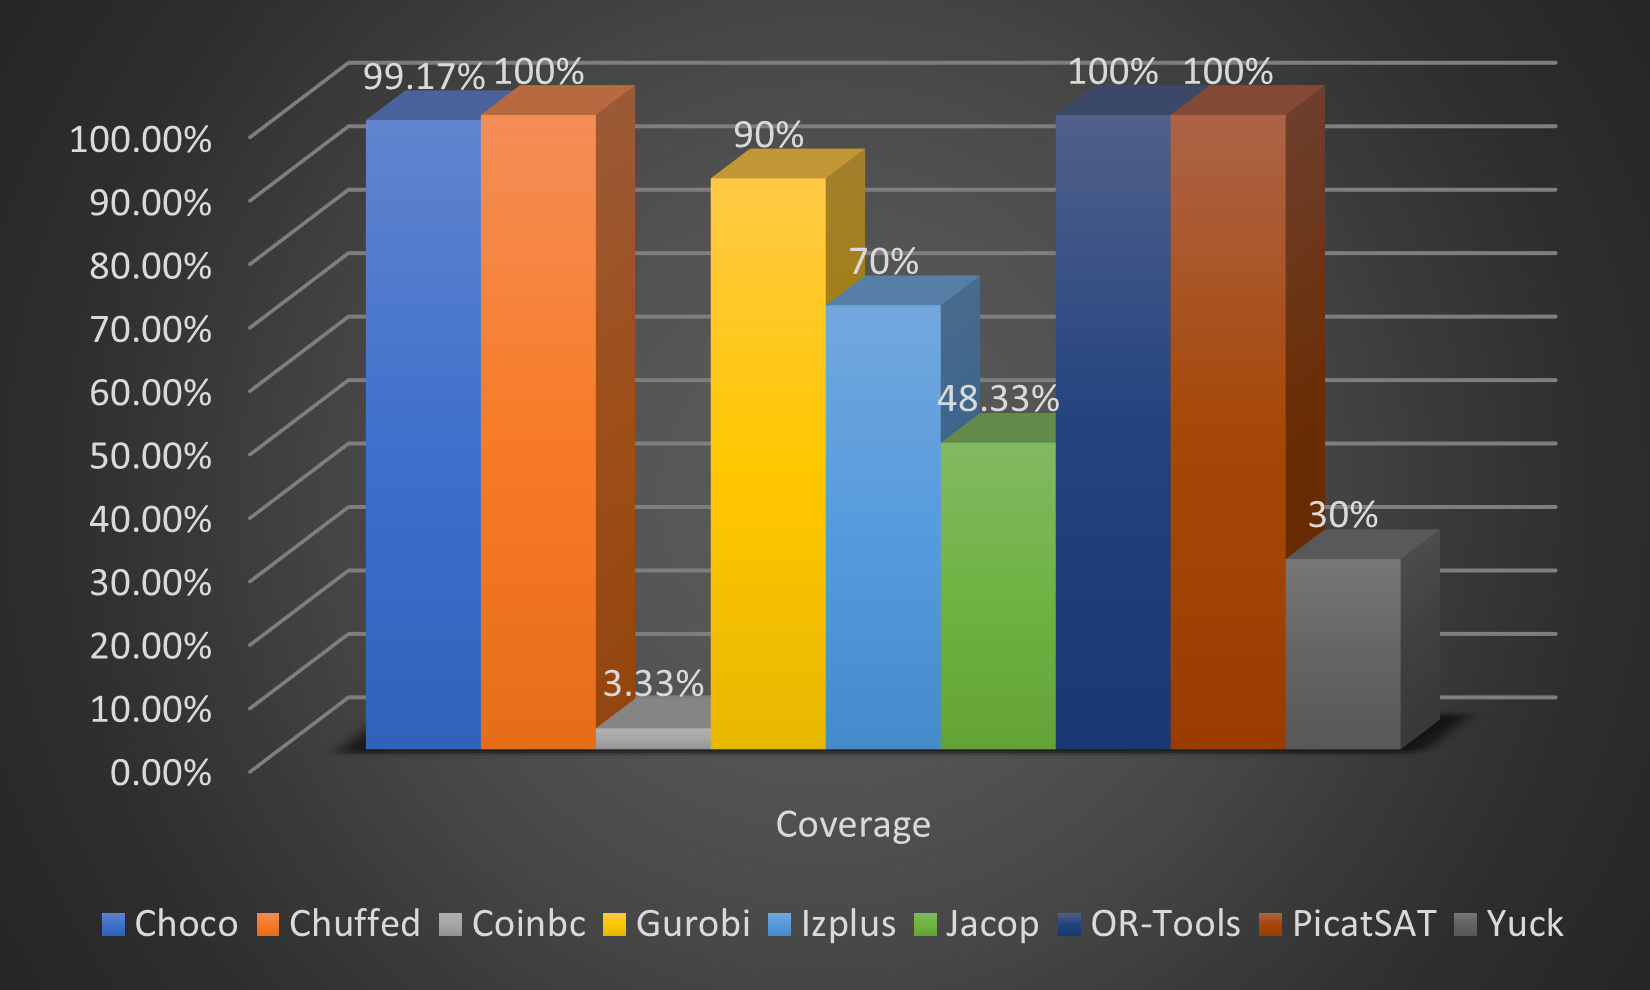
\includegraphics[width=0.8\textwidth]{figs/coverage.png}
    \caption{Overall coverage rates of each solver}
    \label{eva2}
\end{figure}
Table~\ref{tab:solvedproblem} shows the solved problems for each solver. Based on the data in Table~\ref{tab:solvedproblem},
Figure~\ref{eva2} shows the overall coverage rates for different solvers, which indicates that there are only 3 solvers with an overall coverage rate of 100 percent.
In addition, Table~\ref{tab:solvedproblemforeach difficulty} separately shows the solved problems of different difficulties for each solver. 
\begin{table}[htbp]
\centering
\caption{Solved problems of each difficulty (a total of 24 problems for each difficulty)}
\label{tab:solvedproblemforeach difficulty}
\begin{tabular}{|l|l|l|l|l|l|}
\hline
	    &Start&	Junior&	Expert&	Master&	Wizard\\
\hline
Choco   &23   &24 &24 &24 &24\\
\hline
Chuffed	&24   &24 &24 &24 &24\\
\hline
Coinbc	&4    &0  &0  &	0 &0\\
\hline
Gurobi	&24   &22 &20 &	23&19\\
\hline
Izplus	&23   &21 &13 &	17&10\\
\hline
Jacop	&20   &9  &11 &13 &5\\
\hline
OR-Tools	&24   &24 &24 &	24&24\\
\hline
PicatSAT&24   &24 &24 &24 &24\\
\hline
Yuck    &13	  &6  &2  &7  &8\\
\hline
\end{tabular}
\end{table}
Accordingly, Figure~\ref{fig:comparisonIQtwist} illustrates the change of coverage rates as the increase of difficulty. It seems like the other solvers are not stable in different difficulties except there are 3 solvers which always keep 100 percent. In other words, there is no obvious relationship between the coverage and difficulty. Because the method to set the difficulty of IQ Twist is a change of the pegs' positions, and the number of placed pegs has no relationship with difficulty, the change of the number of search nodes is tiny. 
\begin{figure}[H]
    \centering
    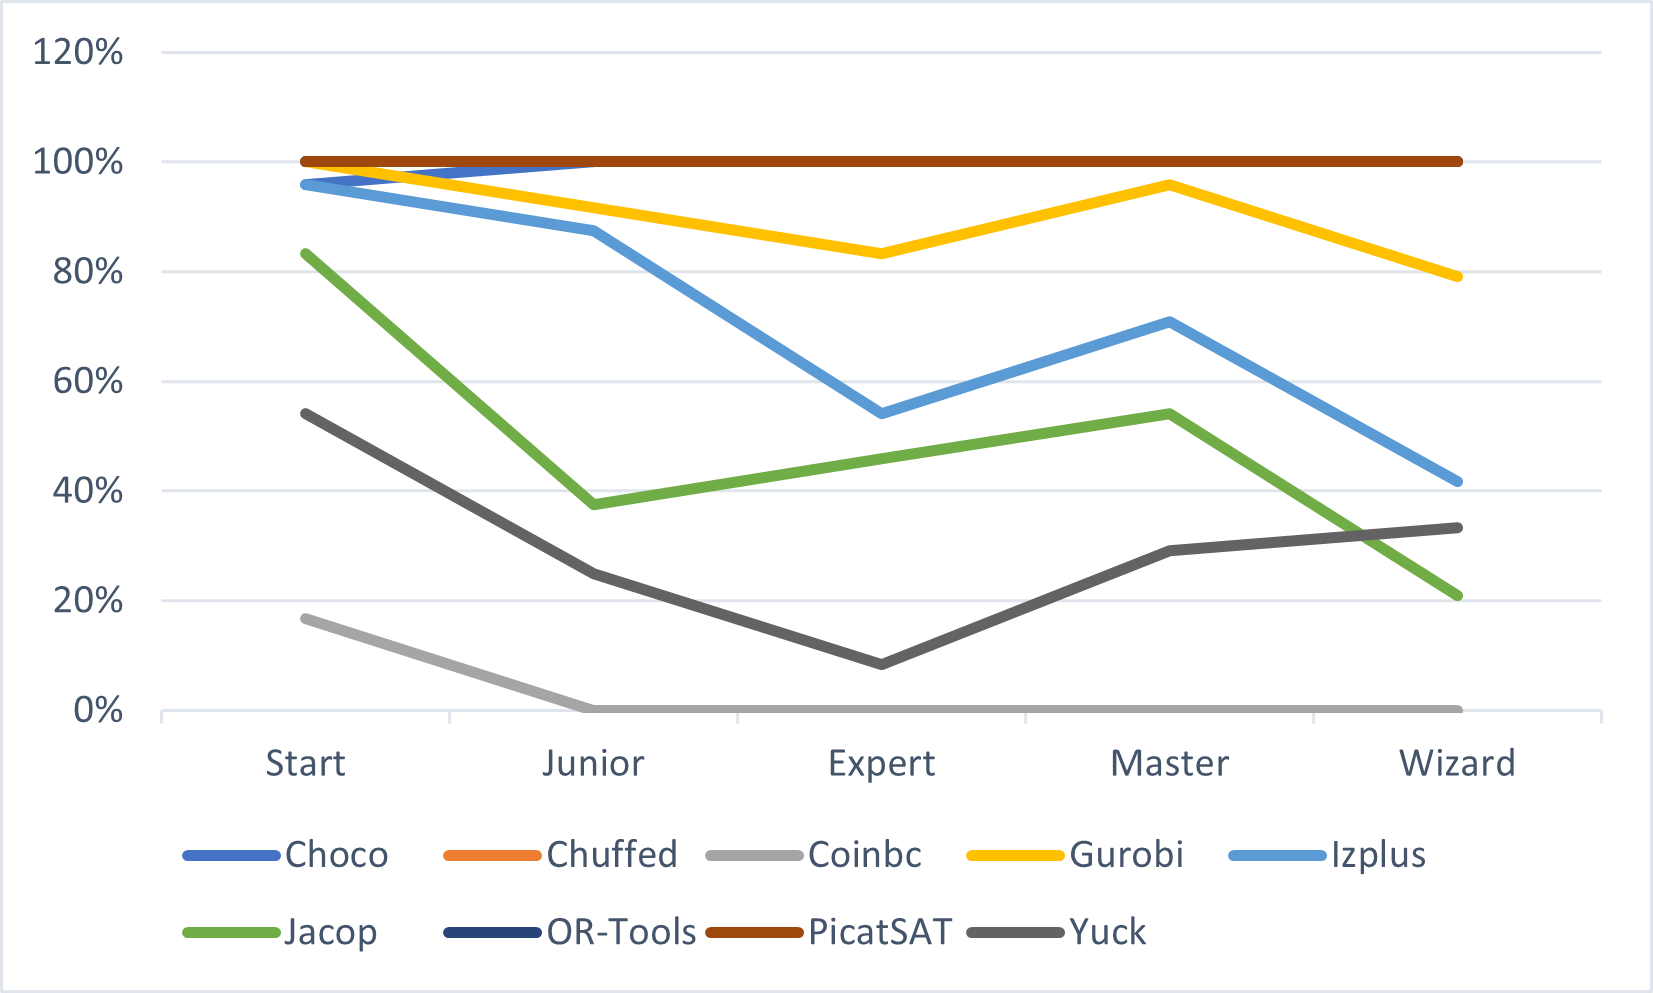
\includegraphics[width=0.8\textwidth]{figs/separated coverage.png}
    \caption{Coverage rates of each difficulty}
    \label{fig:comparisonIQtwist}
\end{figure}
Therefore, compared with other solvers, PicatSAT, OR-Tools and Chuffed take advantage in coverage rates.
\\Secondly, all the execution times have been shown in Figure~\ref{fig:execution times}.
\begin{figure}[H]
    \centering
    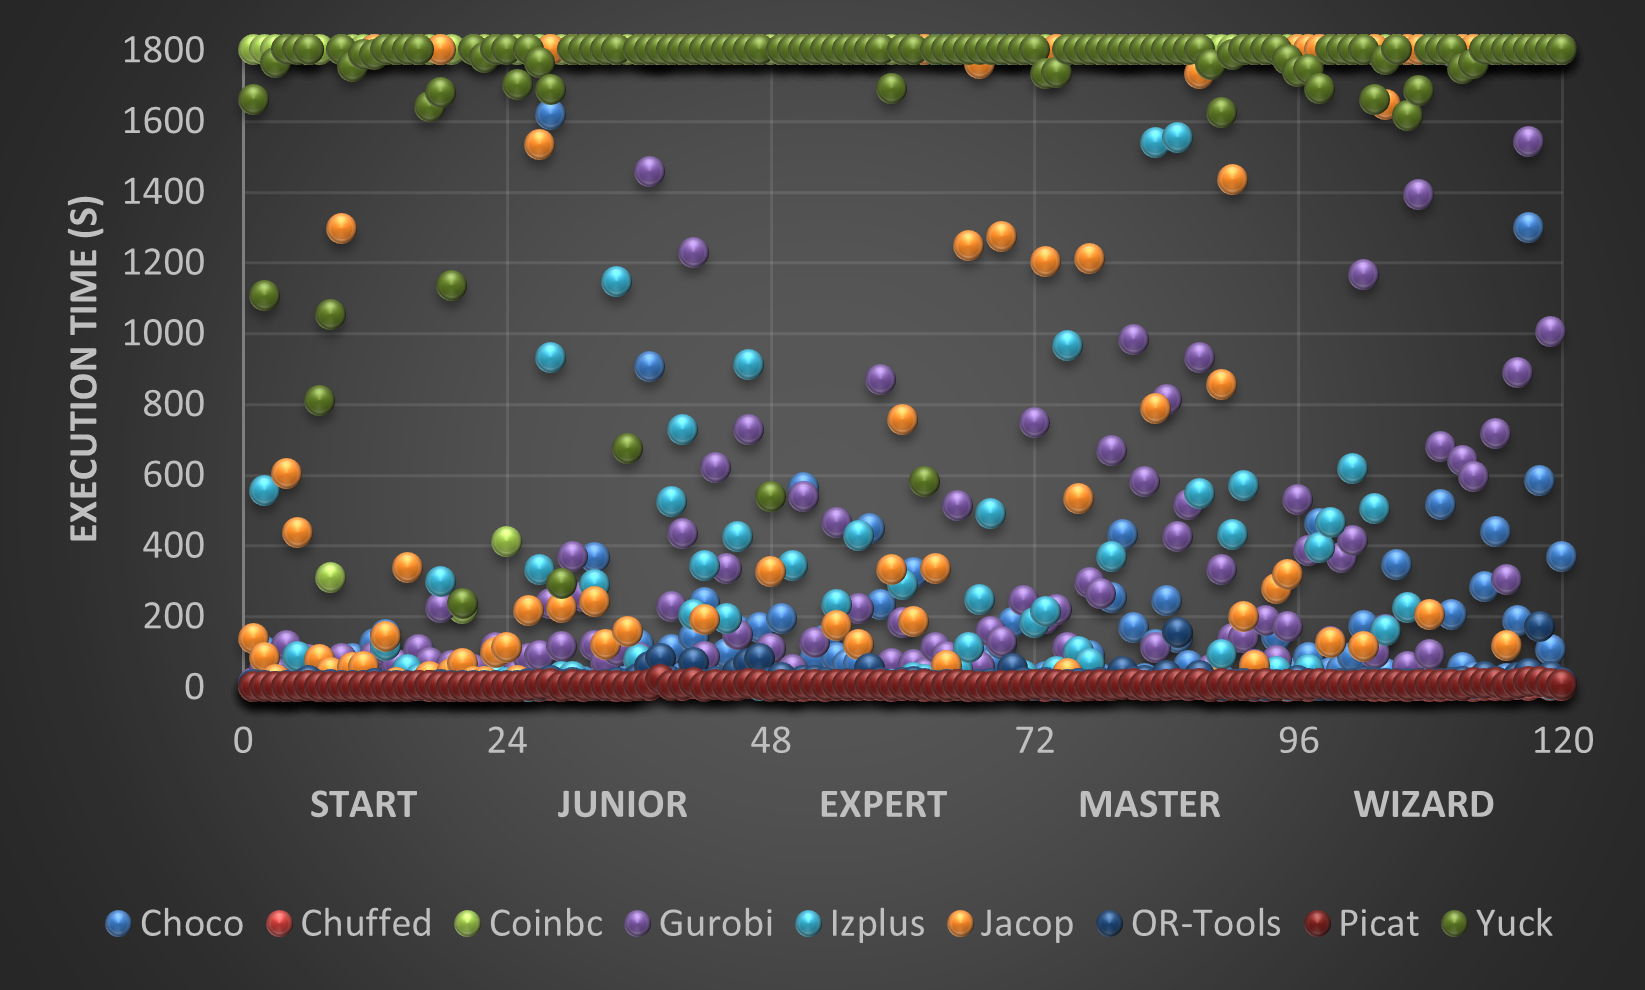
\includegraphics[width=0.8\textwidth]{figs/all_point_IQtwist.png}
    \caption{All execution times of all solvers}
    \label{fig:execution times}
\end{figure}
Figure~\ref{fig:execution times} indicates that Chuffed, PicatSAT and OR-Tools take huge advantages compared with other solvers because the three solvers can solve each problem in only 200 seconds.
\begin{figure}[H]
\centering
\begin{subfigure}[b]{.48\textwidth}
\centering
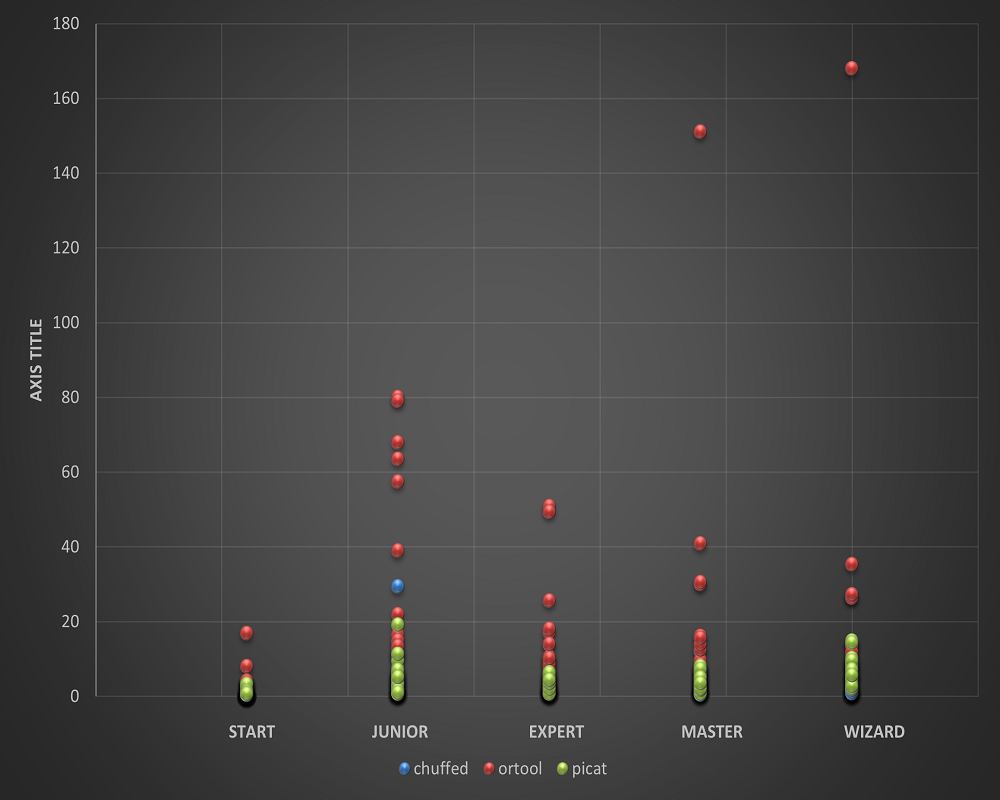
\includegraphics[width=\textwidth]{figs/threesolverpoints.png}
\caption{Execution times for Chuffed, PicatSAT and OR-Tools}
\label{fig:3solvers1}
\end{subfigure}
\begin{subfigure}[b]{.48\textwidth}
\centering
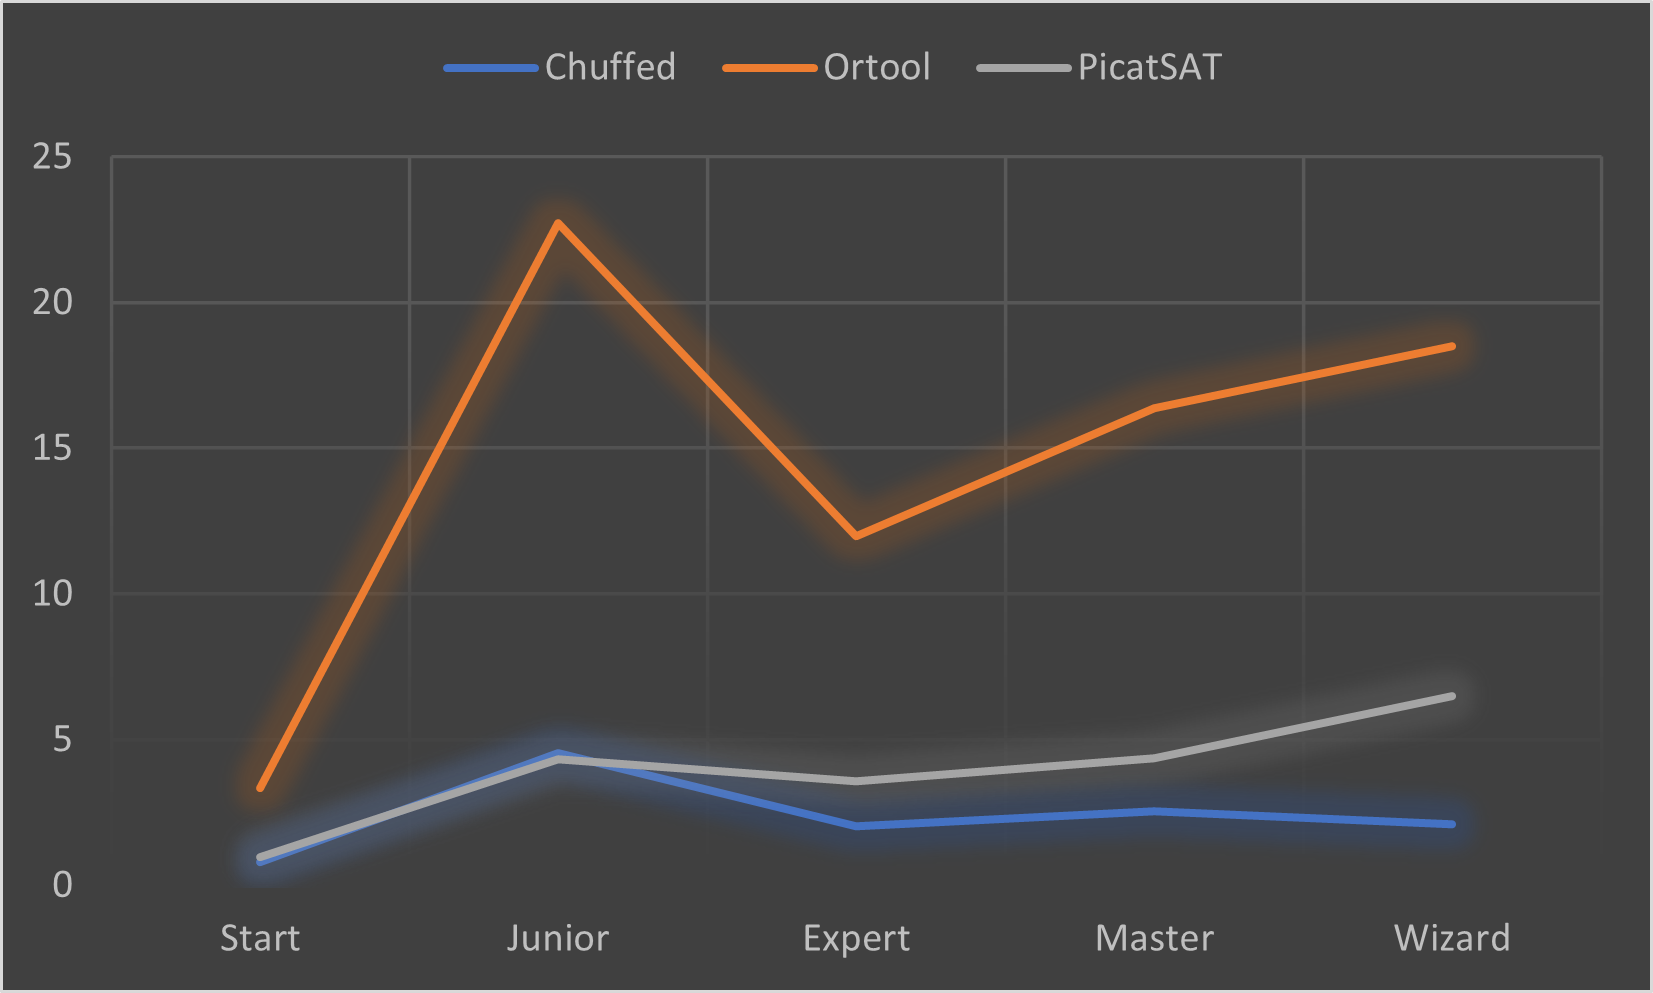
\includegraphics[width=\textwidth]{figs/Three comparison.png}
\caption{Average execution times for Chuffed, PicatSAT and OR-Tools}
\label{fig:3comparison}
\end{subfigure}
\caption{Comparisons between Chuffed, PicatSAT and OR-Tools}
\label{fig:3comparisonsssss}
\end{figure}
Therefore, it is worth to compare the three solvers more closely. Specifically, according to Figure~\ref{fig:3solvers1}, most of the execution times of Chuffed and PicatSAT are close, and they are usually better than OR-Tools.
Furthermore, Figure~\ref{fig:3comparison} indicates that Chuffed spends less time than PicatSAT except in the "junior" difficulty.
\\In short, although all of Chuffed, PicatSAT and OR-Tools can get the result for each problem in 30 minutes, the solver Chuffed possesses the best performance in IQ Twist.
\subsection{Zig Zag Puzzler Results}
\label{sec:Zig Zag Puzzlerresult}
In the Zig Zag Puzzler booklet, there is a total of 80 problems, 40 of them belong to playing mode1, and the other 40 belong to playing mode2. For each playing mode, every 8 problems make up a difficulty level. 
\subsubsection{Playing Mode1}
Firstly, for each solver, we can calculate the coverage rates by Equation~\ref{equation:coverage}.
\begin{table}[htbp]
\centering
\caption{Overall solved problems of each solver for playing mode1 (a total of 40 problems)}
\label{tab:solvedproblem1}
\begin{tabular}{|l|l|l|l|l|l|l|l|l|}
\hline
Choco & Chuffed & Coinbc& Gurobi & Izplus&Jacop& OR-Tools& PicatSAT&Yuck \\
\hline
40   &40      & 20    & 35    &29     &33   &40    &40      &20\\
\hline
\end{tabular}
\end{table}
According to the data in Table~\ref{tab:solvedproblem1}, Figure~\ref{fig:mode1eva2} indicates that there are 4 solvers that keep 100 percent in the overall coverage.
\begin{figure}[H]
     \centering
    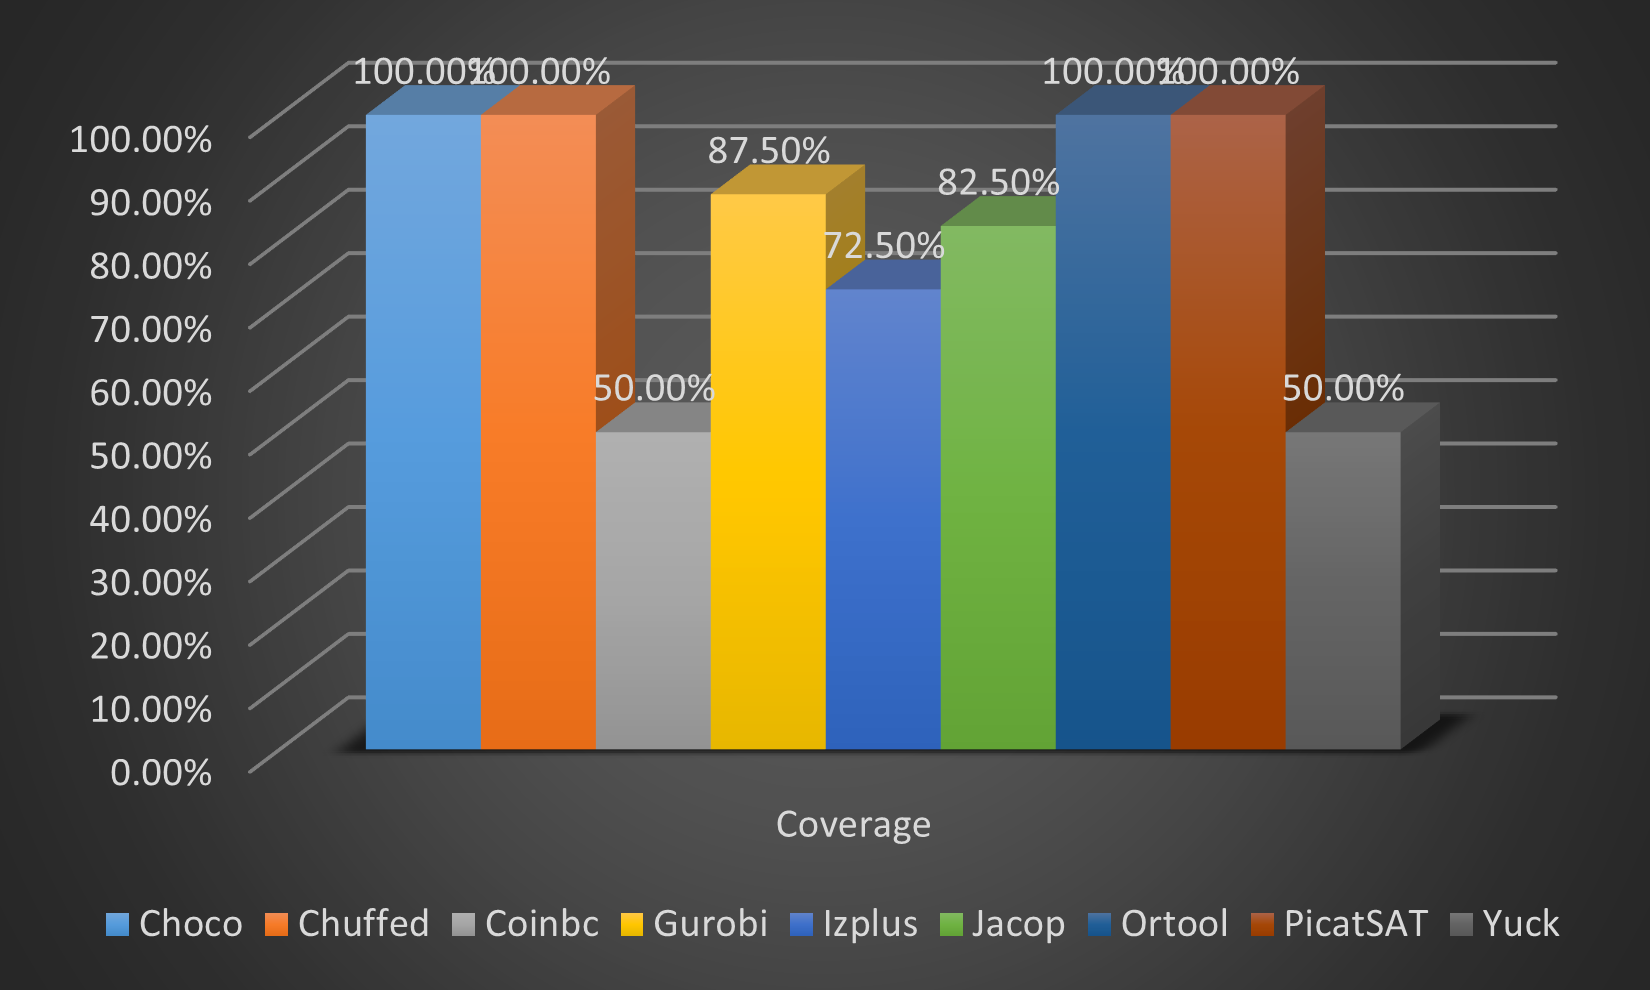
\includegraphics[width=0.8\textwidth]{figs/mode1coverage.png}
    \caption{Overall coverage rates of each solver for playing mode1}
    \label{fig:mode1eva2}
\end{figure}
In addition, on account of Table~\ref{tab:solvedproblemforeach difficulty1}, Figure~\ref{fig:mode1eva4} reveals that except for the four solvers that always keep 100 percent coverage, the other five solvers' separated coverage is decreased as the difficulty increase.
\begin{table}[H]
\centering
\caption{Solved problems for each difficulty in playing mode1 (a total of 8 problems for each difficulty)}
\label{tab:solvedproblemforeach difficulty1}
\begin{tabular}{|l|l|l|l|l|l|}
\hline
	    &Start	&Junior	&Expert	&Master	&Wizard\\
\hline
Choco	&8	&8	&8	&8	&8\\
\hline
Chuffed	&8	&8	&8	&8	&8\\
\hline
Coinbc	&8	&8	&4	&0	&0\\
\hline
Gurobi	&8	&8	&8	&8	&3\\
\hline
Izplus	&8	&8	&8	&4	&1\\
\hline
Jacop	&8	&8	&8	&5	&4\\
\hline
OR-Tools	&8	&8	&8	&8	&8\\
\hline
PicatSAT	&8	&8	&8	&8	&8\\
\hline
Yuck	&8	&8	&4	&0	&0\\
\hline
\end{tabular}
\end{table}
That is quite reasonable because the higher difficulty the fewer placed pieces in this playing mode. The fewer placed pieces means the more search nodes, which causes the solver need more time to find the solution.
\begin{figure}[H]
    \centering
    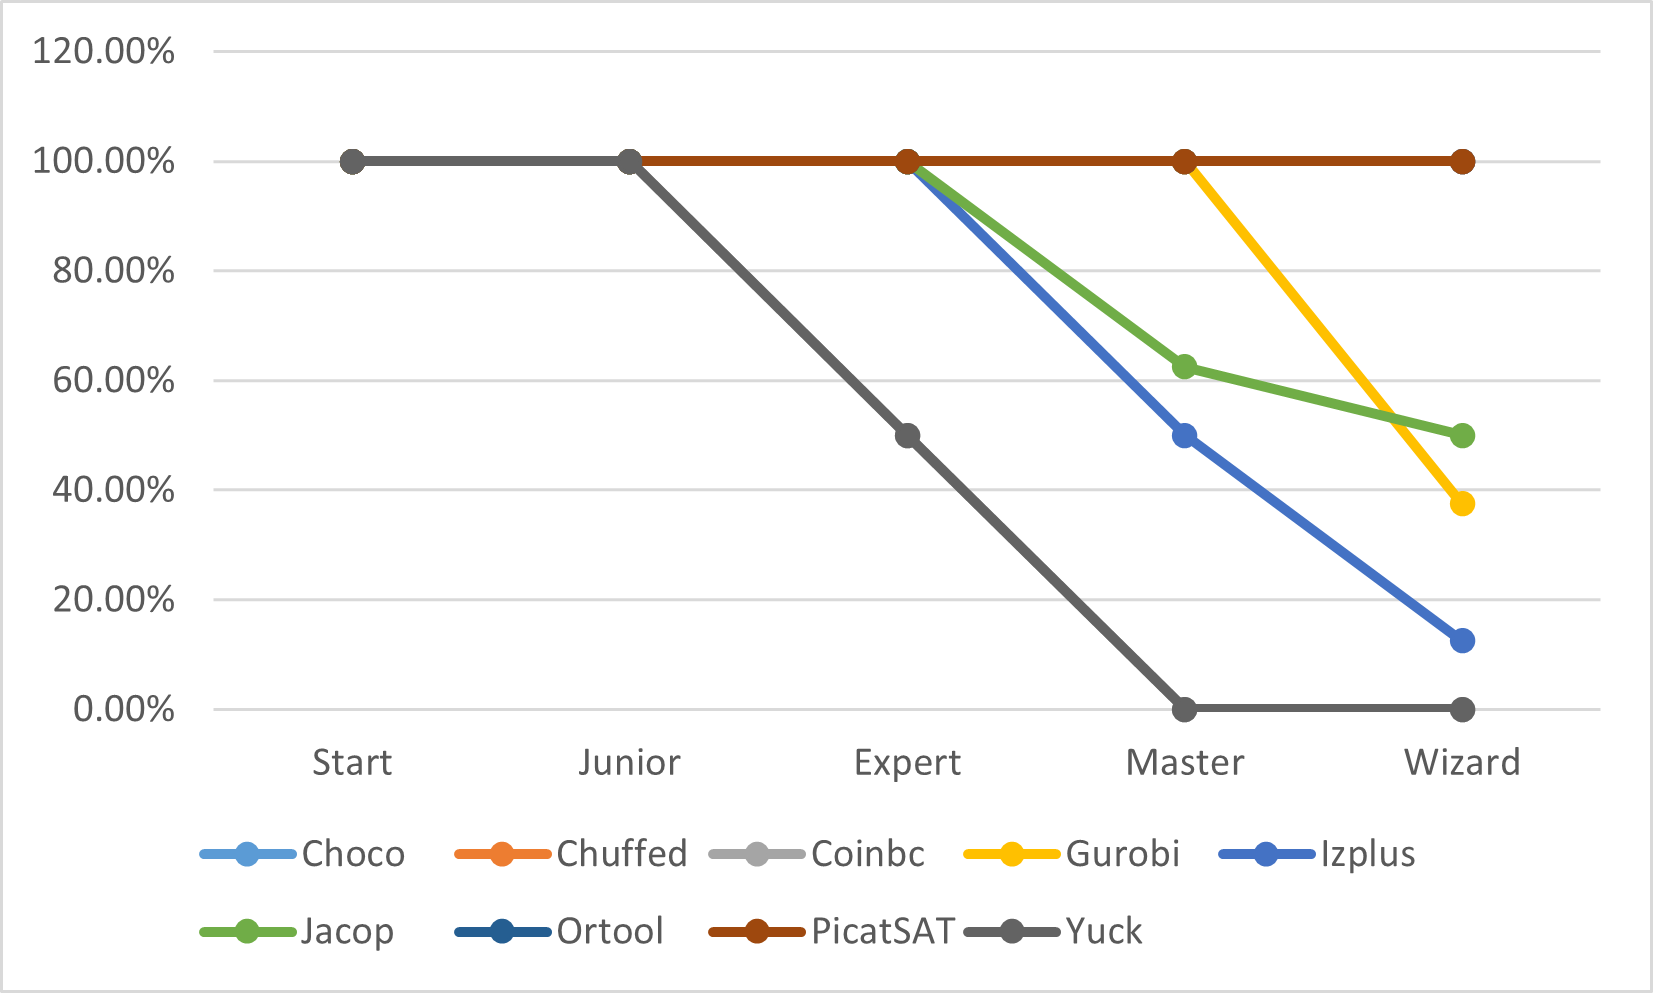
\includegraphics[width=0.8\textwidth]{figs/mode1seperatedcoverage.png}
    \caption{Coverage rates of each difficulty for playing mode1}
    \label{fig:mode1eva4}
\end{figure}
For execution times, Figure~\ref{fig:mode1time1} illustrates that except Choco which spends a lot of time on some problems in  "wizard" difficulty, the other 3 solvers that contain 100 percent overall coverage rates only need a very short time to solve each problem. 
\begin{figure}[htbp]
\centering
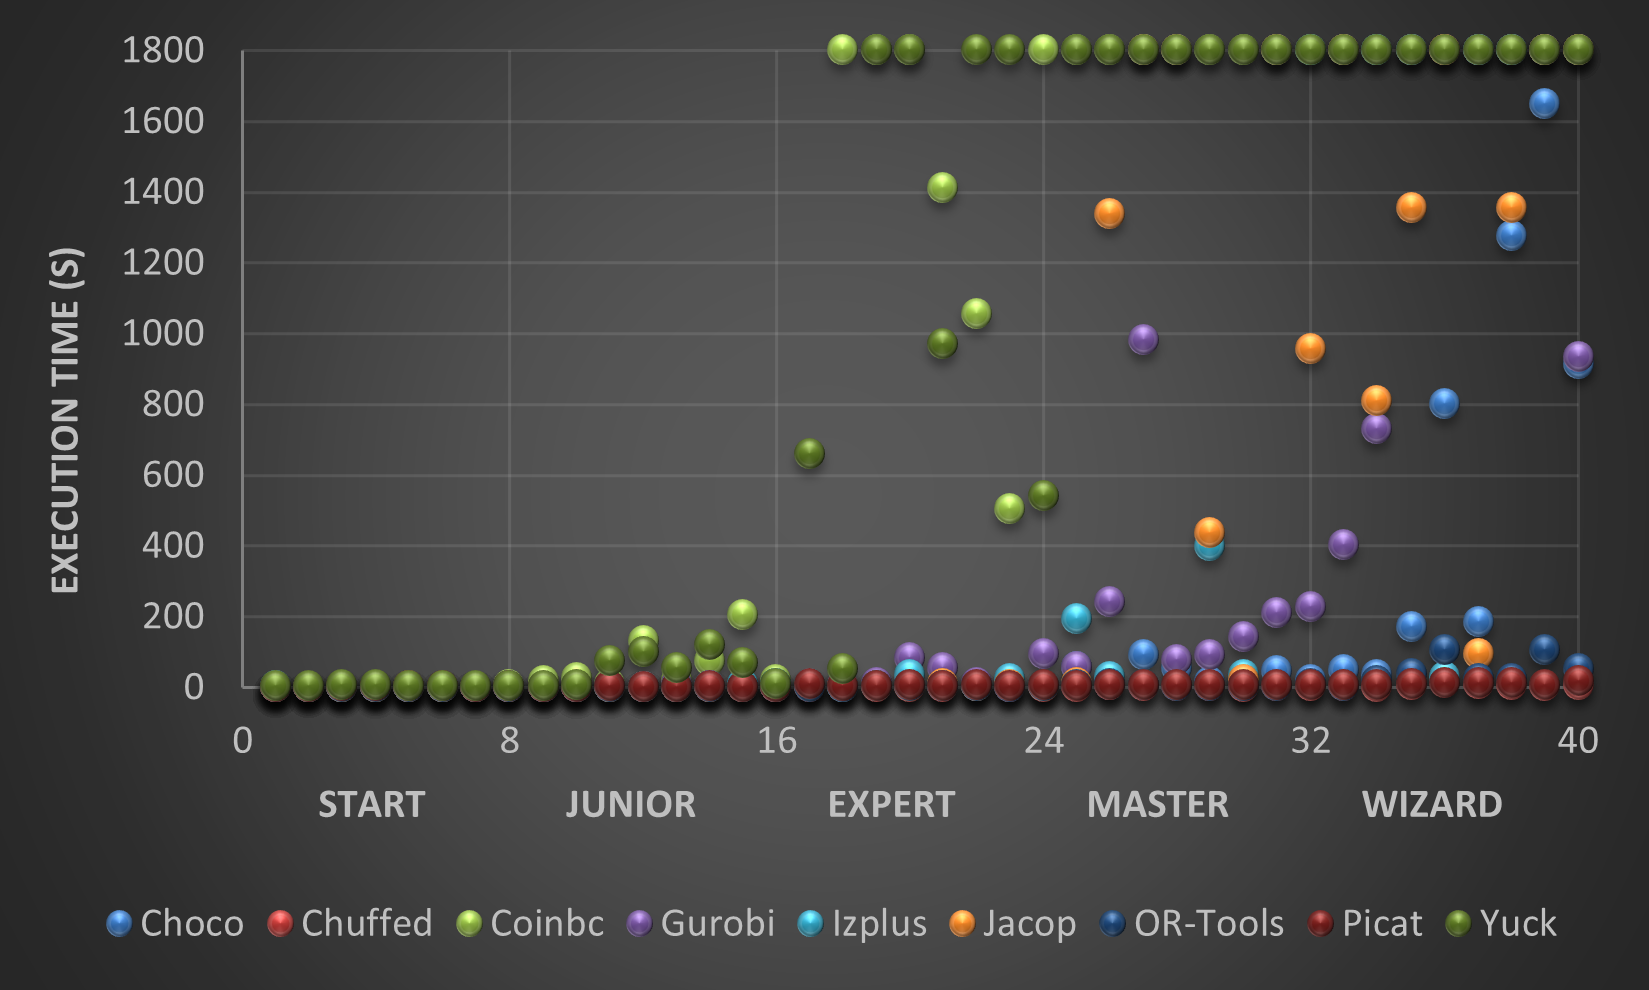
\includegraphics[width=0.8\textwidth]{figs/time1all.png}
\caption{All execution times of all solvers for playing mode1}
\label{fig:mode1time1}
\end{figure}
Moreover, Figure~\ref{fig:time1three} reveals that for the problems in "wizard" difficulty, OR-Tools and PicatSAT spend more time on more problems compared with Chuffed. Accordingly, in Figure~\ref{fig:time1threeslope}, although the start point is very close, the growth rate of slopes for Chuffed is much slower than OR-Tools and PicatSAT. Meanwhile, Figure~\ref{fig:mode1time1} reveals an obvious positive correlation between the execution time of different solvers and the difficulties due to the increased number of search nodes. Therefore, Chuffed has the optimal performance in execution time because of the lowest growth rate of slopes. 
\begin{figure}[htbp]
    \centering
    \begin{subfigure}[b]{0.48\textwidth}
     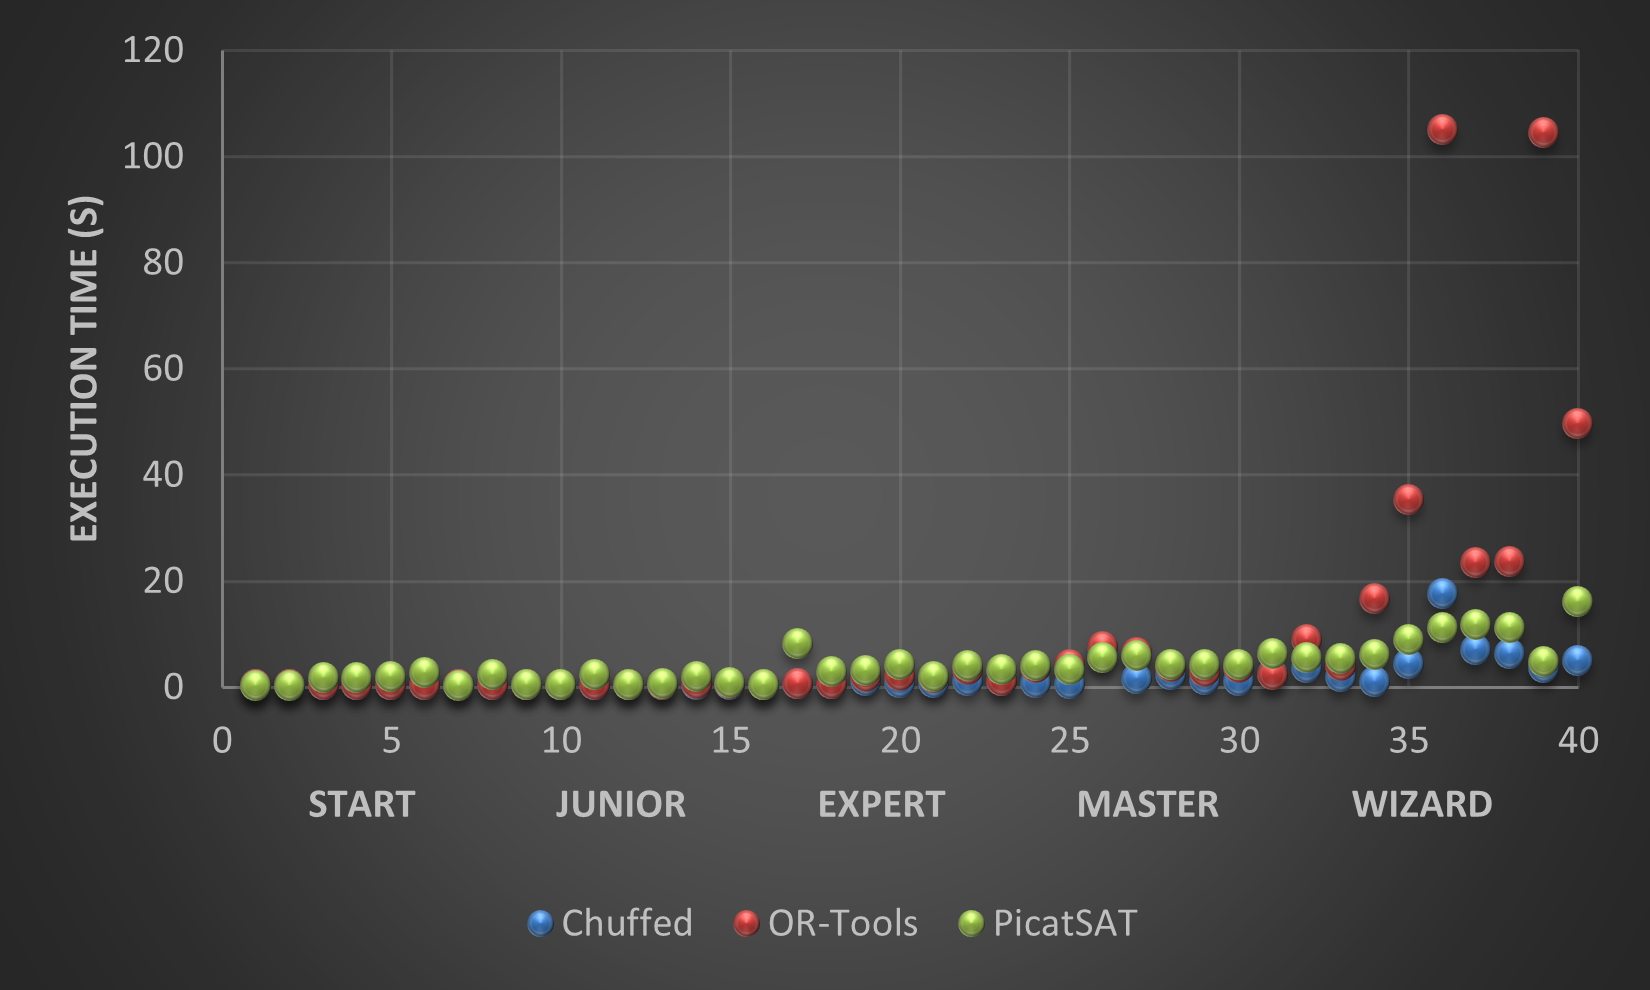
\includegraphics[width=\textwidth]{figs/time1three.png}
    \caption{Execution times for Chuffed, PicatSAT and OR-Tools}
    \label{fig:time1three}
    \end{subfigure}
    \begin{subfigure}[b]{0.48\textwidth}
     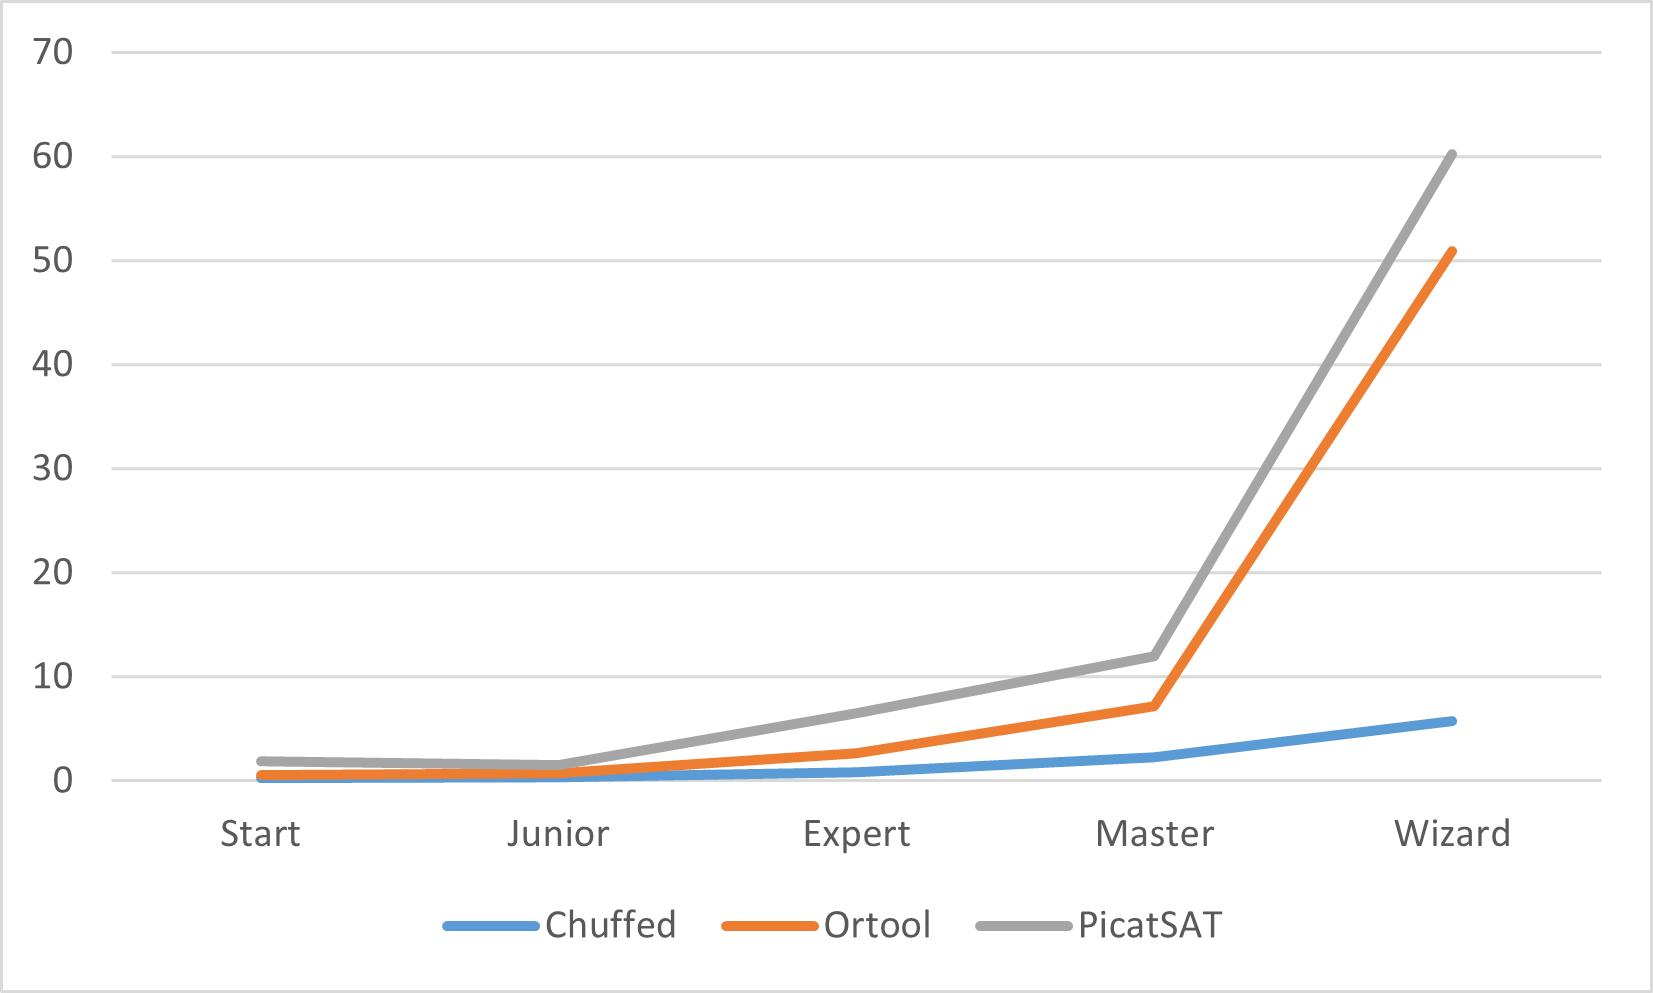
\includegraphics[width=\textwidth]{figs/mode1solverscomparison.png}
    \caption{Average execution time for Chuffed, PicatSAT and OR-Tools}
    \label{fig:time1threeslope}
    \end{subfigure}
    \caption{Comparisons between Chuffed, PicatSAT and OR-Tools for playing mode1}
\end{figure}
Overall, combine coverage and execution times, Chuffed possesses the best performance in Zig Zag Puzzler playing mode1.
\subsubsection{Playing Mode2}
\begin{table}[H]
\centering
\caption{Overall solved problems of each solver for playing mode2 (a total of 40 problems)}
\label{tab:solvedproblem2}
\begin{tabular}{|l|l|l|l|l|l|l|l|l|}
\hline
Choco & Chuffed & Coinbc& Gurobi & Izplus&Jacop& OR-Tools& PicatSAT&Yuck \\
\hline
37   &40      & 12    & 34    &35     &32   &40    &40      &22\\
\hline
\end{tabular}
\end{table}
Based on Table~\ref{tab:solvedproblem2}, as is shown in Figure~\ref{fig:mode2eva2}, the result of coverage rates is quite similar to the result of coverage rates in playing mode 1 because the rule of playing mode2 is quite similar with playing mode1. Both of them set fewer pieces as difficulty increases.
\begin{figure}[H]
     \centering
    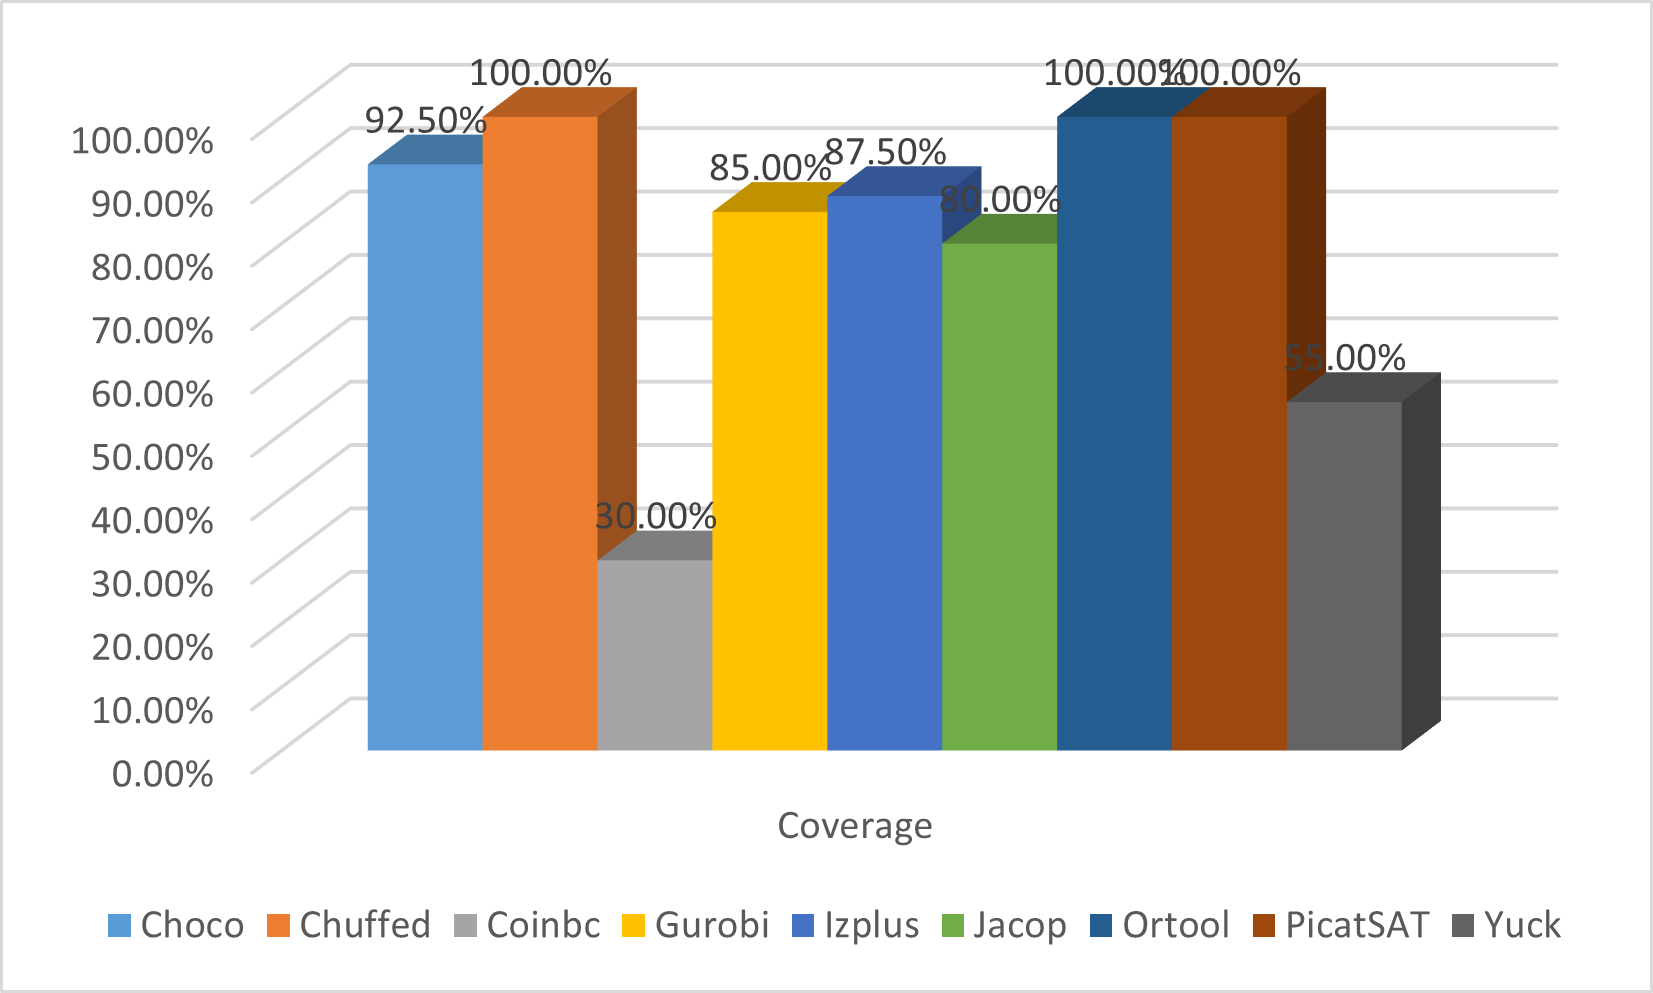
\includegraphics[width=0.8\textwidth]{figs/mode2coverage.png}
    \caption{Overall coverage rates of each solver for playing mode2}
    \label{fig:mode2eva2}
\end{figure}
Again, Chuffed, PicatSAT and OR-Tools solve each problem in 30 minutes. 
\begin{table}[H]
\centering
\caption{Solved problems of each difficulty for playing mode2 (a total of 8 problems for each difficulty)}
\label{tab:solvedproblemforeach difficulty2}
\begin{tabular}{|l|l|l|l|l|l|}
\hline
	    &Start	&Junior	&Expert	&Master	&Wizard\\
\hline
Choco	&8	&8	&8	&8	&5\\
\hline
Chuffed	&8	&8	&8	&8	&8\\
\hline
Coinbc	&7	&5	&0	&0	&0\\
\hline
Gurobi	&8	&8	&8	&7	&3\\
\hline
Izplus	&8	&8	&8	&7	&4\\
\hline
Jacop	&8	&8	&8	&7	&1\\
\hline
OR-Tools	&8	&8	&8	&8	&8\\
\hline
PicatSAT	&8	&8	&8	&8	&8\\
\hline
Yuck	&8	&8	&4	&2	&0\\
\hline
\end{tabular}
\end{table}
Meanwhile, according to the data in Table~\ref{tab:solvedproblemforeach difficulty2}, Figure~\ref{fig:mode2eva4} indicates that the other 6 solvers' separated coverage is decreased as the difficulty increases, which is also very similar with playing mode1.
 \begin{figure}[H]
   \centering
    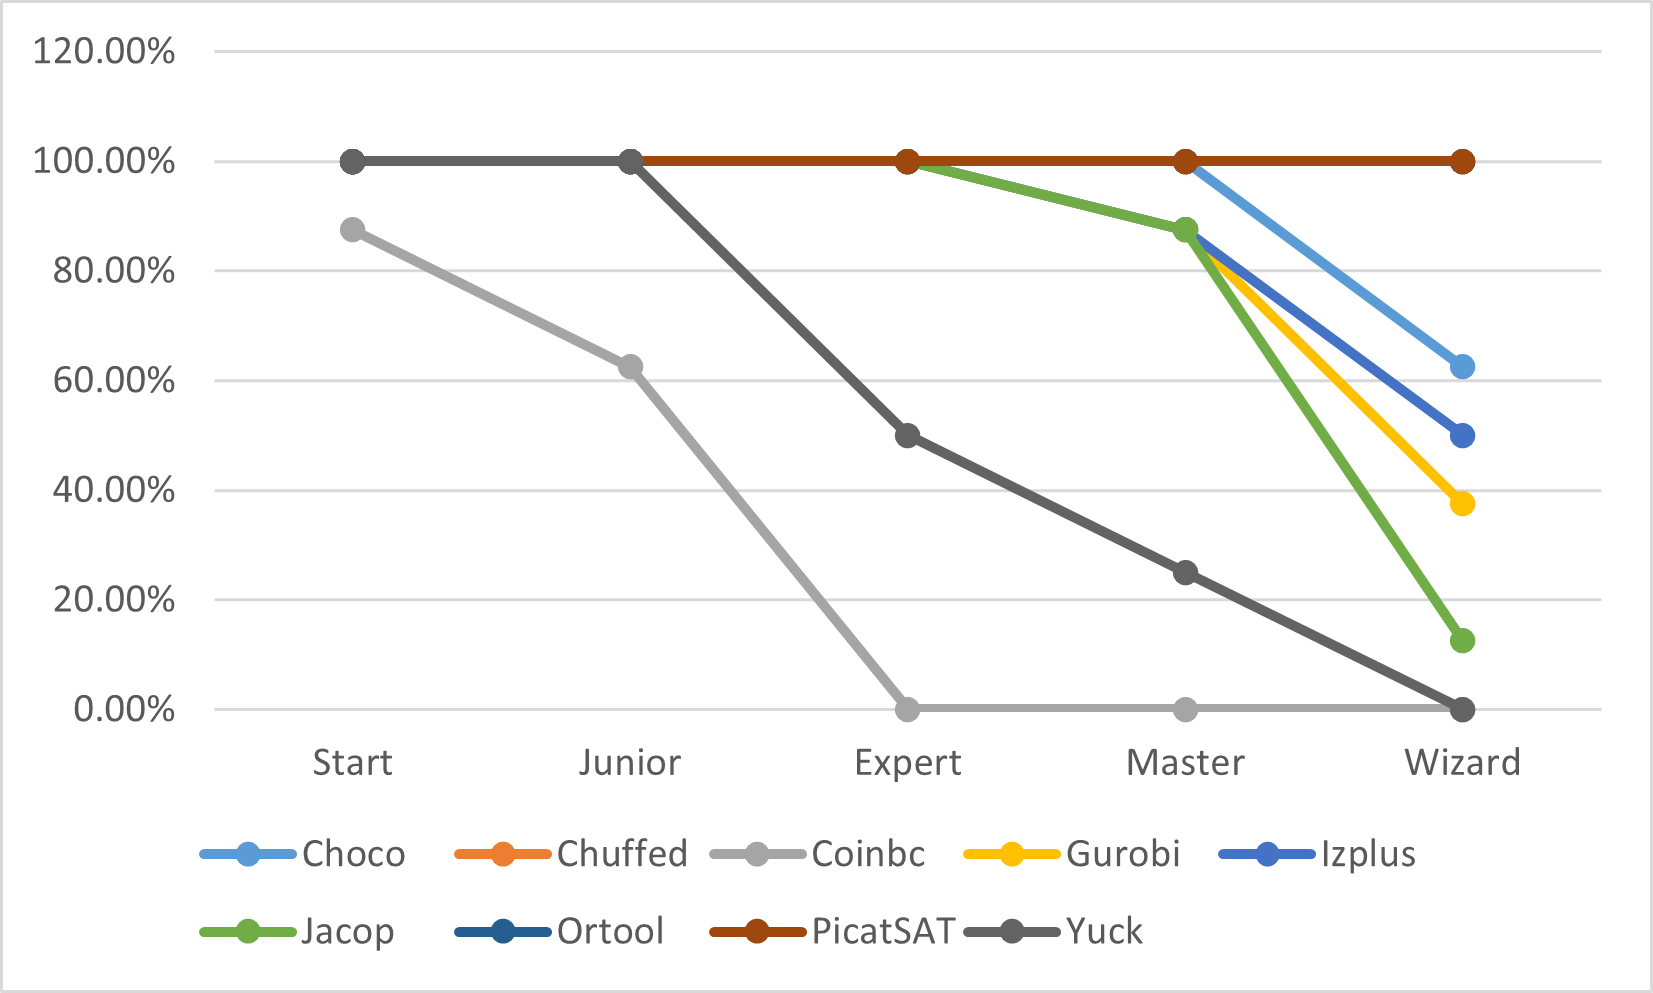
\includegraphics[width=0.8\textwidth]{figs/mode2seperatedcoverage.png}
    \caption{Coverage rates of each difficulty in playing mode2}
    \label{fig:mode2eva4}
\end{figure}
For the execution times, as is shown in Figure~\ref{fig:mode2time2}, almost all the solvers' execution times are a positive correlation with the difficulties. Again, Chuffed, PicatSAT and OR-Tools spend less time to solve most problems. 
\begin{figure}[H]
    \centering
    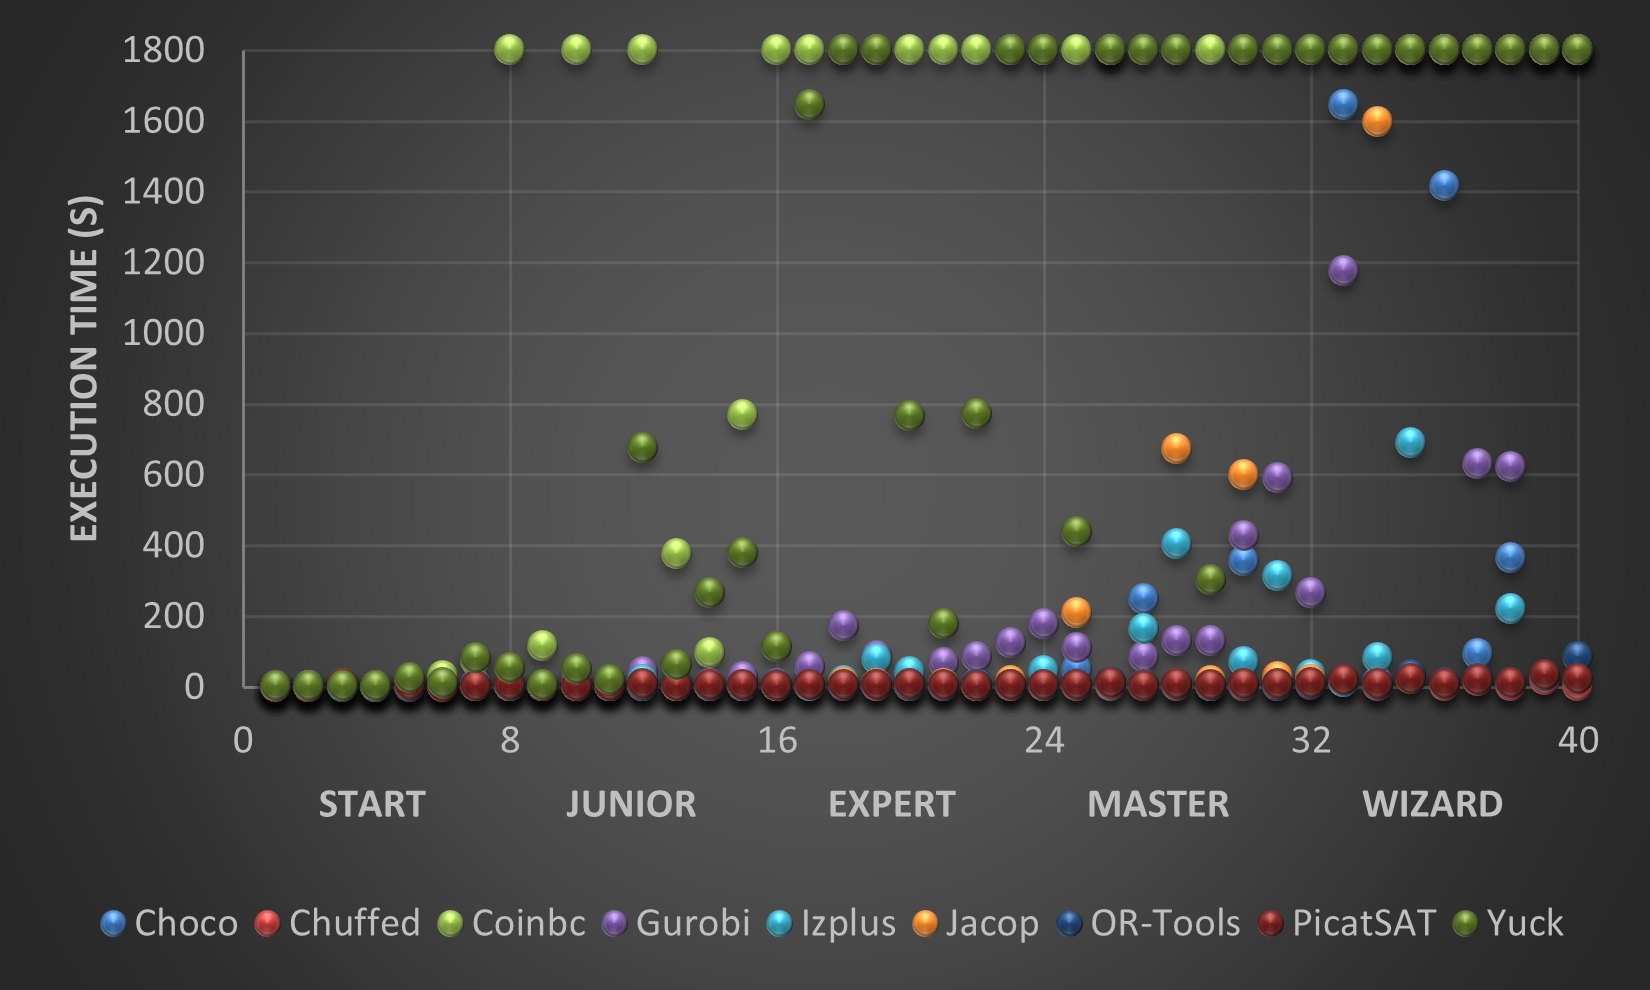
\includegraphics[width=0.8\textwidth]{figs/time2all.png}
    \caption{All execution times of all solvers for playing mode2}
    \label{fig:mode2time2}
\end{figure}
Similarly, on account of Figure~\ref{fig:comparisonlast}, Chuffed achieves optimal performance. 
\begin{figure}[H]
\begin{subfigure}[b]{0.48\textwidth}
  \centering
    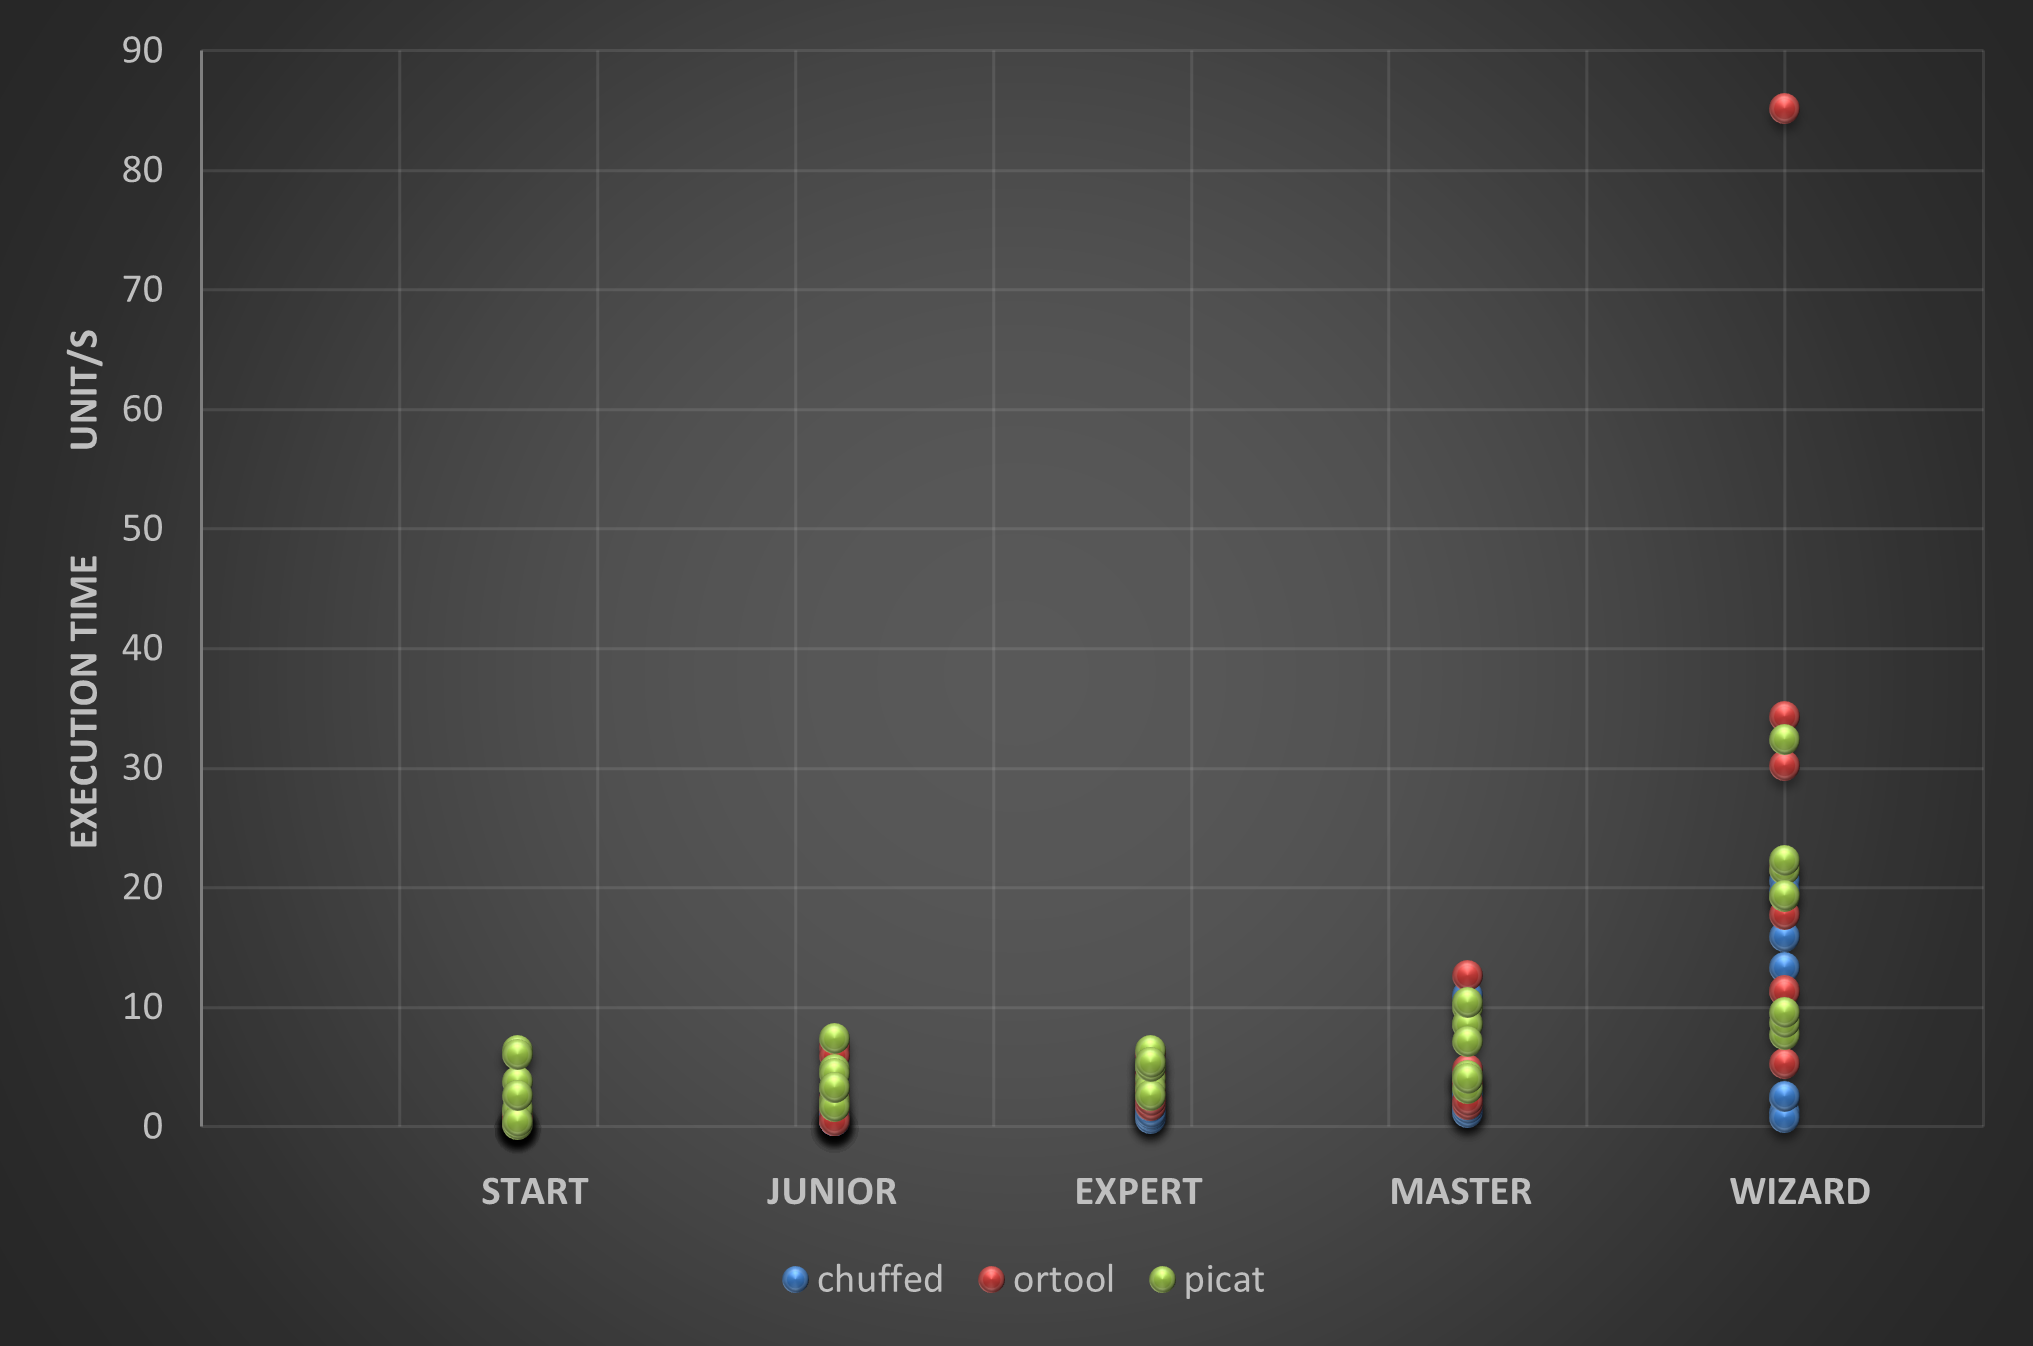
\includegraphics[width=\textwidth]{figs/time2three.png}
    \caption{Execution times for Chuffed, PicatSAT and OR-Tools}
    \label{fig:compare}
\end{subfigure}
\begin{subfigure}[b]{0.48\textwidth}
 \centering
    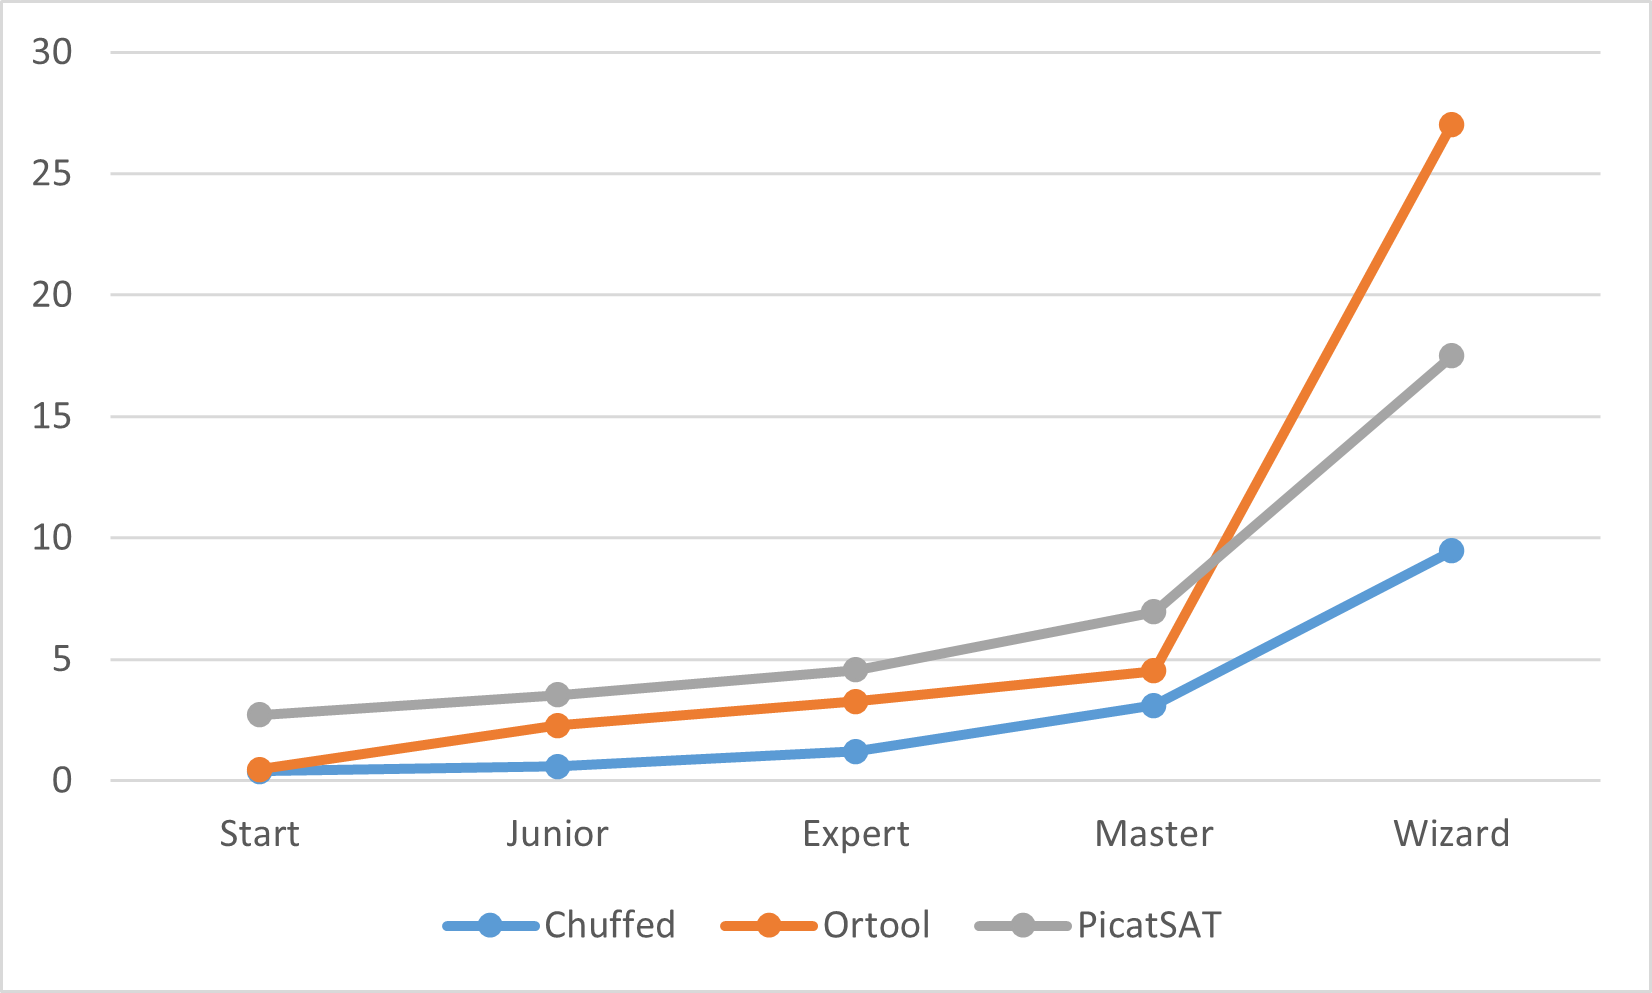
\includegraphics[width=\textwidth]{figs/Threecomparison2.png}
    \caption{Average execution times for Chuffed, PicatSAT and OR-Tools}
    \label{fig:compare}
\end{subfigure}
\caption{Comparisons between Chuffed, PicatSAT and OR-Tools for playing mode2}
\label{fig:comparisonlast}
\end{figure}
\subsection{Summary}
\label{sec:Summary}
The difficulty setting in IQ Twist and Zig Zag Puzzler are quite different, which causes the relationship between solvers' performance and difficulty are very different. However, for Zig Zag Puzzler, because both playing modes set fewer pieces as the increase of difficulty, the relationships between solvers' performance and the games' difficulty level are very similar. In addition, for all the problems in both IQ Twist and Zig Zag Puzzler, Chuffed, PicatSAT and OR-Tools can solve each of them in 30 minutes. Meanwhile, their performances are more stable and the average execution times for all problems are only a few seconds. To sum up, compared with other solvers, Chuffed, PicatSAT and OR-Tools have obvious advantages in such problems, moreover, Chuffed cost the shortest time in most problems. 
 
\chapter{Conclusion}
\label{cha:conc}
There are 120 problems created for IQ Twist, and 80 problems created for Zig Zag Puzzler through Minizinc. All of these problems come from the game booklets. After the creations of these problems, nine solvers that are based on different languages are used to evaluate each problem. Finally, the coverage rates of each solver and the execution time for each problem by different solvers have been discussed, which indicates that the Chuffed, PicatSAT and OR-Tools can cover all the problems, meanwhile, they need shorter execution time for solving most problems. In addition, Chuffed achieves the optimal performance because even for the highest difficulty, it solves each problem in 20 seconds for both games. In comparison, the other two solvers usually need more execution time in each difficulty for both games. And with the increase of difficulty, the advantage of Chuffed in execution time becomes more significant. 
\section{Future Work}
\label{sec:future}
In the future, I would like to figure out why Chuffed, PicatSAT and OR-Tools can cover all the problems in a short time. Some of their features have been mentioned in Chapter~\ref{section:compiler}. 
For Chuffed, the reasons why lazy clause generation and nogood logbook can achieve such an optimal performance might be interesting. 
For OR-Tools, what the combination optimization methods of OR-Tools are and why they can achieve good performance are worth considering.
For PicatSAT, the Picat language and the advantages of log encoding may be worth learning.
Of course, except for the features that I mentioned, there might be other special parts of each solver. After figures out their advantages, I may try to create another solver that combines their advantages.





%%%%%%%%%%%%%%%%%%%%%%%%%%%%%%%%%%%%%%%%%%%%%%%%%%%%%%%%%%%%%%%%%%%%%%
% Here begins the end matter

\backmatter

%%%%%%%%%%%%%%%%%%%%%%%%%%%%%%%%%%%%%%%%%%%%%%%%%%%%%%%%%%%%%%%%%%%%%%
%% Bibliography
\cleardoublepage
\phantomsection
\bibliographystyle{IEEEtran}
\bibliography{report}
\begin{appendices}
\section{IQtwist pieces' constraints}
\label{appendix:2Dpieces}
\begin{itemize}
  \item piece Yellow1\\
  \begin{align*}
&\Con{y11}{y12}{y13}=\\
\{&((x_{1},y_{1}),(x_{2},y_{2}),(x_{3},y_{3}))\in \Domain{y11}\times \Domain{y12}\times\Domain{y13}\mid\\
&(x_{2} = x_{1} + 1,\hspace{1ex}y_{2} = y_{1},\hspace{1ex}x_{3} = x_{1} + 2, \hspace{1ex}y_{3} = y_{1})\hspace{1ex} or\\
&(x_{2} = x_{1},\hspace{1ex}y_{2} = y_{1}+1,\hspace{1ex}x_{3} = x_{1}, \hspace{1ex}y_{3} = y_{1}+2)\hspace{1ex} or\\
&(x_{2} = x_{1}-1,\hspace{1ex}y_{2} = y_{1},\hspace{1ex}x_{3} = x_{1}-2,\hspace{1ex} y_{3} = y_{1})\hspace{1ex} or\\
&(x_{2} = x_{1},\hspace{1ex}y_{2} = y_{1}-1,\hspace{1ex}x_{3} = x_{1}, \hspace{1ex}y_{3} = y_{1}-2)\hspace{3ex} \}
\end{align*} 
  \item piece Blue1 
  \begin{align*}
&\Cons{b11}{b12}{b13}{b14}{b15}=
\\\{&((x_{1},y_{1}),(x_{2},y_{2}),(x_{3},y_{3}),(x_{4},y_{4}),(x_{5},y_{5}))\in \\
&\Domain {b11} \times \Domain{b12}\times \Domain{b13}\times \Domain{b14}\times \Domain{b15} \mid\\
&(x_{2} = x_{1},\hspace{1ex}y_{2} = y_{1}+1,\hspace{1ex}x_{3} = x_{1}+1,\hspace{1ex}y_{3} = y_{1}+1,
\\&x_{4} = x_{1},\hspace{1ex}y_{4} = y_{1}+2,\hspace{1ex}x_{5} = x_{1}+1,\hspace{1ex}y_{5} = y_{1}+2)\hspace{1ex} or \\
&(x_{2} = x_{1}-1 ,\hspace{1ex}y_{2} = y_{1},\hspace{1ex}x_{3} = x_{1}-1,\hspace{1ex}y_{3} = y_{1}+1,
\\&x_{4} = x_{1}-2,\hspace{1ex}y_{4} = y_{1},\hspace{1ex}x_{5} = x_{1}-2,\hspace{1ex}y_{5} = y_{1}+1)\hspace{1ex} or \\
&(x_{2} = x_{1} ,\hspace{1ex}y_{2} = y_{1}-1,\hspace{1ex}x_{3} = x_{1}-1,\hspace{1ex}y_{3} = y_{1}-1,
\\&x_{4} = x_{1},\hspace{1ex}y_{4} = y_{1}-2,\hspace{1ex}x_{5} = x_{1}-1,\hspace{1ex}y_{5} = y_{1}-2)\hspace{1ex} or \\
&(x_{2} = x_{1}+1 ,\hspace{1ex}y_{2} = y_{1},\hspace{1ex}x_{3} = x_{1}+1,\hspace{1ex}y_{3} = y_{1}-1,
\\&x_{4} = x_{1}+2,\hspace{1ex}y_{4} = y_{1},\hspace{1ex}x_{5} = x_{1}+2,\hspace{1ex}y_{5} = y_{1}-1)\hspace{1ex} or \\
&(x_{2} = x_{1},\hspace{1ex}y_{2} = y_{1}+1,\hspace{1ex}x_{3} = x_{1}-1,\hspace{1ex}y_{3} = y_{1}+1,
\\&x_{4} = x_{1},\hspace{1ex}y_{4} = y_{1}+2,\hspace{1ex}x_{5} = x_{1}-1,\hspace{1ex}y_{5} = y_{1}+2)\hspace{1ex} or \\
&(x_{2} = x_{1}-1 ,\hspace{1ex}y_{2} = y_{1},\hspace{1ex}x_{3} = x_{1}-1,\hspace{1ex}y_{3} = y_{1}-1,
\\&x_{4} = x_{1}-2,\hspace{1ex}y_{4} = y_{1},\hspace{1ex}x_{5} = x_{1}-2,\hspace{1ex}y_{5} = y_{1}-1)\hspace{1ex} or \\
&(x_{2} = x_{1} ,\hspace{1ex}y_{2} = y_{1}-1,\hspace{1ex}x_{3} = x_{1}+1,\hspace{1ex}y_{3} = y_{1}-1,
\\&x_{4} = x_{1},\hspace{1ex}y_{4} = y_{1}-2,\hspace{1ex}x_{5} = x_{1}+1,\hspace{1ex}y_{5} = y_{1}-2)\hspace{1ex} or \\
&(x_{2} = x_{1}+1 ,\hspace{1ex}y_{2} = y_{1},\hspace{1ex}x_{3} = x_{1}+1,\hspace{1ex}y_{3} = y_{1}+1,
\\&x_{4} = x_{1}+2,\hspace{1ex}y_{4} = y_{1},\hspace{1ex}x_{5} = x_{1}+2,\hspace{1ex}y_{5} = y_{1}+1)\hspace{3ex}\}
\end{align*}  
  \item piece Blue2\\
  \begin{align*}
&\Const{b21}{b22}{b23}{b24}=\\
\{&((x_{1},y_{1}),(x_{2},y_{2}),(x_{3},y_{3}),(x_{4},y_{4}))\in \Domain{b21}\times \Domain{b22}\times\Domain{b23}\times\Domain{b24}\mid\\
&(x_{2} = x_{1} + 1,\hspace{1ex}y_{2} = y_{1},\hspace{1ex}x_{3} = x_{1} + 2, \hspace{1ex}y_{3} = y_{1},\hspace{1ex}x_{4} = x_{1}+3,\hspace{1ex}y_{4} = y_{1})\hspace{1ex} or\\
&(x_{2} = x_{1},\hspace{1ex}y_{2} = y_{1}+1,\hspace{1ex}x_{3} = x_{1}, \hspace{1ex}y_{3} = y_{1}+2,\hspace{1ex}x_{4} = x_{1},\hspace{1ex}y_{4} = y_{1}+3)\hspace{1ex} or\\
&(x_{2} = x_{1}-1,\hspace{1ex}y_{2} = y_{1},\hspace{1ex}x_{3} = x_{1}-2,\hspace{1ex} y_{3} = y_{1},\hspace{1ex}x_{4} = x_{1}-3,\hspace{1ex}y_{4} = y_{1})\hspace{1ex} or\\
&(x_{2} = x_{1},\hspace{1ex}y_{2} = y_{1}-1,\hspace{1ex}x_{3} = x_{1}, \hspace{1ex}y_{3} = y_{1}-2,\hspace{1ex}x_{4} = x_{1},\hspace{1ex}y_{4} = y_{1}-3)\hspace{3ex} \}
\end{align*}
 \item piece Green1\\
 \begin{align*}
&\Const{g11}{g12}{g13}{g14}=
\\\{&((x_{1},y_{1}),(x_{2},y_{2}),(x_{3},y_{3}),(x_{4},y_{4}))\in \Domain{g11}\times \Domain{g12}\times\Domain{g13}\times\Domain{g14}\mid\\
&(x_{2} = x_{1} + 1,\hspace{1ex}y_{2} = y_{1},\hspace{1ex}x_{3} = x_{1} + 2, \hspace{1ex}y_{3} = y_{1},\hspace{1ex}x_{4} = x_{1}+1,\hspace{1ex}y_{4} = y_{1}+1)\hspace{1ex} or\\
&(x_{2} = x_{1},\hspace{1ex}y_{2} = y_{1}+1,\hspace{1ex}x_{3} = x_{1}, \hspace{1ex}y_{3} = y_{1}+2,\hspace{1ex}x_{4} = x_{1}-1,\hspace{1ex}y_{4} = y_{1}+1)\hspace{1ex} or\\
&(x_{2} = x_{1}-1,\hspace{1ex}y_{2} = y_{1},\hspace{1ex}x_{3} = x_{1}-2,\hspace{1ex} y_{3} = y_{1},\hspace{1ex}x_{4} = x_{1}-1,\hspace{1ex}y_{4} = y_{1}-1)\hspace{1ex} or\\
&(x_{2} = x_{1},\hspace{1ex}y_{2} = y_{1}-1,\hspace{1ex}x_{3} = x_{1}, \hspace{1ex}y_{3} = y_{1}-2,\hspace{1ex}x_{4} = x_{1}+1,\hspace{1ex}y_{4} = y_{1}-1)\hspace{1ex} or\\
&(x_{2} = x_{1}-1,\hspace{1ex}y_{2} = y_{1},\hspace{1ex}x_{3} = x_{1}-2, \hspace{1ex}y_{3} = y_{1},\hspace{1ex}x_{4} = x_{1}-1,\hspace{1ex}y_{4} = y_{1}-1)\hspace{1ex} or\\
&(x_{2} = x_{1},\hspace{1ex}y_{2} = y_{1}-1,\hspace{1ex}x_{3} = x_{1}, \hspace{1ex}y_{3} = y_{1}-2,\hspace{1ex}x_{4} = x_{1}-1,\hspace{1ex}y_{4} = y_{1}-1)\hspace{1ex} or\\
&(x_{2} = x_{1}+1,\hspace{1ex}y_{2} = y_{1},\hspace{1ex}x_{3} = x_{1}+2, \hspace{1ex}y_{3} = y_{1},\hspace{1ex}x_{4} = x_{1}+1,\hspace{1ex}y_{4} = y_{1}-1)\hspace{1ex} or\\
&(x_{2} = x_{1},\hspace{1ex}y_{2} = y_{1}+1,\hspace{1ex}x_{3} = x_{1}, \hspace{1ex}y_{3} = y_{1}+2,\hspace{1ex}x_{4} = x_{1}+1,\hspace{1ex}y_{4} = y_{1}+1)\hspace{3ex} \}
\end{align*}
 \item piece Green2\\
 \begin{align*}
&\Con{g21}{g22}{g23}=
\\\{&((x_{1},y_{1}),(x_{2},y_{2}),(x_{3},y_{3}))\in \Domain{g21}\times \Domain{g22}\times\Domain{g23}\mid\\
&(x_{2} = x_{1}+1,\hspace{1ex}y_{2} = y_{1},\hspace{1ex}x_{3} = x_{1}+1, \hspace{1ex}y_{3} = y_{1}+1)\hspace{1ex} or\\
&(x_{2} = x_{1},\hspace{1ex}y_{2} = y_{1}+1,\hspace{1ex}x_{3} = x_{1}-1, \hspace{1ex}y_{3} = y_{1}+1)\hspace{1ex} or\\
&(x_{2} = x_{1}-1,\hspace{1ex}y_{2} = y_{1},\hspace{1ex}x_{3} = x_{1}-1,\hspace{1ex} y_{3} = y_{1}-1)\hspace{1ex} or\\
&(x_{2} = x_{1},\hspace{1ex}y_{2} = y_{1}-1,\hspace{1ex}x_{3} = x_{1}+1, \hspace{1ex}y_{3} = y_{1}-1)\hspace{1ex} or\\
&(x_{2} = x_{1}-1,\hspace{1ex}y_{2} = y_{1},\hspace{1ex}x_{3} = x_{1}-1, \hspace{1ex}y_{3} = y_{1}+1)\hspace{1ex} or\\
&(x_{2} = x_{1},\hspace{1ex}y_{2} = y_{1}-1,\hspace{1ex}x_{3} = x_{1}-1, \hspace{1ex}y_{3} = y_{1}-1)\hspace{1ex} or\\
&(x_{2} = x_{1}+1,\hspace{1ex}y_{2} = y_{1},\hspace{1ex}x_{3} = x_{1}+1, \hspace{1ex}y_{3} = y_{1}-1)\hspace{1ex} or\\
&(x_{2} = x_{1},\hspace{1ex}y_{2} = y_{1}+1,\hspace{1ex}x_{3} = x_{1}+1, \hspace{1ex}y_{3} = y_{1}+1) \hspace{3ex} \}
\end{align*}
\item piece Red1 
\begin{align*}
&\Const{r11}{r12}{r13}{r14}=\\
\{&((x_{1},y_{1}),(x_{2},y_{2}),(x_{3},y_{3}),(x_{4},y_{4}))\in 
\\&\Domain{r11}\times \Domain{r12}\times\Domain{r13}\times\Domain{r14}\mid\\
&(x_{2} = x_{1} + 1,\hspace{1ex}y_{2} = y_{1},\hspace{1ex}x_{3} = x_{1} + 1, 
\\&y_{3} = y_{1}+1,\hspace{1ex}x_{4} = x_{1}+2,\hspace{1ex}y_{4} = y_{1}+1)\hspace{1ex} or\\
&(x_{2} = x_{1},\hspace{1ex}y_{2} = y_{1}+1,\hspace{1ex}x_{3} = x_{1}-1, 
\\&y_{3} = y_{1}+1,\hspace{1ex}x_{4} = x_{1}-1,\hspace{1ex}y_{4} = y_{1}+2)\hspace{1ex} or\\
&(x_{2} = x_{1}-1,\hspace{1ex}y_{2} = y_{1},\hspace{1ex}x_{3} = x_{1}-1,
\\&y_{3} = y_{1}-1,\hspace{1ex}x_{4} = x_{1}-2,\hspace{1ex}y_{4} = y_{1}-1)\hspace{1ex} or\\
&(x_{2} = x_{1},\hspace{1ex}y_{2} = y_{1}-1,\hspace{1ex}x_{3} = x_{1}+1, 
\\&y_{3} = y_{1}-1,\hspace{1ex}x_{4} = x_{1}+1,\hspace{1ex}y_{4} = y_{1}-2)\hspace{1ex} or\\
&(x_{2} = x_{1}-1,\hspace{1ex}y_{2} = y_{1},\hspace{1ex}x_{3} = x_{1}-1, 
\\&y_{3} = y_{1}+1,\hspace{1ex}x_{4} = x_{1}-2,\hspace{1ex}y_{4} = y_{1}+1)\hspace{1ex} or\\
&(x_{2} = x_{1},\hspace{1ex}y_{2} = y_{1}-1,\hspace{1ex}x_{3} = x_{1}-1, 
\\&y_{3} = y_{1}-1,\hspace{1ex}x_{4} = x_{1}-1,\hspace{1ex}y_{4} = y_{1}-2)\hspace{1ex} or\\
&(x_{2} = x_{1}+1,\hspace{1ex}y_{2} = y_{1},\hspace{1ex}x_{3} = x_{1}+1, 
\\&y_{3} = y_{1}-1,\hspace{1ex}x_{4} = x_{1}+2,\hspace{1ex}y_{4} = y_{1}-1)\hspace{1ex} or\\
&(x_{2} = x_{1},\hspace{1ex}y_{2} = y_{1}+1,\hspace{1ex}x_{3} = x_{1}+1, 
\\&y_{3} = y_{1}+1,\hspace{1ex}x_{4} = x_{1}+1,\hspace{1ex}y_{4} = y_{1}+2)\hspace{3ex} \} 
\end{align*}
\item piece Red2\\
\begin{align*}
&\Const{r21}{r22}{r23}{r24}=
\\\{&((x_{1},y_{1}),(x_{2},y_{2}),(x_{3},y_{3}),(x_{4},y_{4}))\in \Domain{r21}\times \Domain{r22}\times\Domain{r23}\times\Domain{r24}\mid\\
&(x_{2} = x_{1} + 1,\hspace{1ex}y_{2} = y_{1},\hspace{1ex}x_{3} = x_{1} + 2, \hspace{1ex}y_{3} = y_{1},\hspace{1ex}x_{4} = x_{1},\hspace{1ex}y_{4} = y_{1}+1)\hspace{1ex} or\\
&(x_{2} = x_{1},\hspace{1ex}y_{2} = y_{1}+1,\hspace{1ex}x_{3} = x_{1}, \hspace{1ex}y_{3} = y_{1}+2,\hspace{1ex}x_{4} = x_{1}-1,\hspace{1ex}y_{4} = y_{1})\hspace{1ex} or\\
&(x_{2} = x_{1}-1,\hspace{1ex}y_{2} = y_{1},\hspace{1ex}x_{3} = x_{1}-2,\hspace{1ex} y_{3} = y_{1},\hspace{1ex}x_{4} = x_{1},\hspace{1ex}y_{4} = y_{1}-1)\hspace{1ex} or\\
&(x_{2} = x_{1},\hspace{1ex}y_{2} = y_{1}-1,\hspace{1ex}x_{3} = x_{1}, \hspace{1ex}y_{3} = y_{1}-2,\hspace{1ex}x_{4} = x_{1}+1,\hspace{1ex}y_{4} = y_{1})\hspace{1ex} or\\
&(x_{2} = x_{1}-1,\hspace{1ex}y_{2} = y_{1},\hspace{1ex}x_{3} = x_{1}-2, \hspace{1ex}y_{3} = y_{1},\hspace{1ex}x_{4} = x_{1},\hspace{1ex}y_{4} = y_{1}+1)\hspace{1ex} or\\
&(x_{2} = x_{1},\hspace{1ex}y_{2} = y_{1}-1,\hspace{1ex}x_{3} = x_{1}, \hspace{1ex}y_{3} = y_{1}-2,\hspace{1ex}x_{4} = x_{1}-1,\hspace{1ex}y_{4} = y_{1})\hspace{1ex} or\\
&(x_{2} = x_{1}+1,\hspace{1ex}y_{2} = y_{1},\hspace{1ex}x_{3} = x_{1}+2, \hspace{1ex}y_{3} = y_{1},\hspace{1ex}x_{4} = x_{1},\hspace{1ex}y_{4} = y_{1}-1)\hspace{1ex} or\\
&(x_{2} = x_{1},\hspace{1ex}y_{2} = y_{1}+1,\hspace{1ex}x_{3} = x_{1}, \hspace{1ex}y_{3} = y_{1}+2,\hspace{1ex}x_{4} = x_{1}+1,\hspace{1ex}y_{4} = y_{1})\hspace{3ex} \} 
\end{align*}
\end{itemize}

\section{IQtwist pegs' constraints}
\label{appendix:2Dpegs}
\begin{itemize}
  \item Yellow peg1\\
  \begin{align*}  
\Constraint{py1} = &\{((x_{1},y_{1}),(x_{2},y_{2}))\in \Domain{py1} \times \Domain{y11}\mid x_{2} = x_{1} \hspace{1ex} , \hspace{1ex}  y_{2} = y_{1}\}\hspace{1ex} \cup  
\\&\{((x_{1},y_{1}),(x_{2},y_{2}))\in \Domain{py1} \times \Domain{y21}\mid x_{2} = x_{1} \hspace{1ex} , \hspace{1ex}  y_{2} = y_{1}\}\hspace{1ex} \cup 
\\&\{ ((x_{1},y_{1}),(x_{2},y_{2}))\in \Domain{py1} \times \Domain{y22}\mid x_{2} = x_{1} \hspace{1ex} , \hspace{1ex}  y_{2} = y_{1}\}\hspace{1ex}\cup 
\\& \{((x_{1},y_{1}),(x_{2},y_{2}))\in \Domain{py1} \times \Domain{y24}\mid x_{2} = x_{1} \hspace{1ex} , \hspace{1ex}  y_{2} = y_{1}\} \hspace{1ex}\cup
\\& \{(0,0)\}
\end{align*}
  \item Yellow peg2\\
  \begin{align*}
\Constraint{py2} = &\{((x_{1},y_{1}),(x_{2},y_{2}))\in \Domain{py2} \times \Domain{y11}\mid x_{2} = x_{1} \hspace{1ex} , \hspace{1ex}  y_{2} = y_{1}\} \hspace{1ex} \cup 
\\& \{((x_{1},y_{1}),(x_{2},y_{2}))\in \Domain{py2} \times \Domain{y21}\mid x_{2} = x_{1} \hspace{1ex} , \hspace{1ex}  y_{2} = y_{1}\} \hspace{1ex} \cup 
\\& \{ ((x_{1},y_{1}),(x_{2},y_{2}))\in \Domain{py2} \times \Domain{y22}\mid x_{2} = x_{1} \hspace{1ex} , \hspace{1ex}  y_{2} = y_{1}\} \hspace{1ex} \cup 
\\&\{((x_{1},y_{1}),(x_{2},y_{2}))\in \Domain{py2} \times \Domain{y24}\mid x_{2} = x_{1} \hspace{1ex} , \hspace{1ex}  y_{2} = y_{1}\} \hspace{1ex}\cup
\\& \{(0,0)\}
\end{align*}
  \item Blue peg1\\
  \begin{align*}
\Constraint{pb1} = &\{((x_{1},y_{1}),(x_{2},y_{2}))\in \Domain{pb1} \times \Domain{b13}\mid x_{2} = x_{1} \hspace{1ex} , \hspace{1ex}  y_{2} = y_{1}\} \hspace{1ex} \cup 
\\& \{((x_{1},y_{1}),(x_{2},y_{2}))\in \Domain{pb1} \times \Domain{b15}\mid x_{2} = x_{1} \hspace{1ex} , \hspace{1ex}  y_{2} = y_{1}\} \hspace{1ex} \cup 
\\& \{ ((x_{1},y_{1}),(x_{2},y_{2}))\in \Domain{pb1} \times \Domain{b23}\mid x_{2} = x_{1} \hspace{1ex} , \hspace{1ex}  y_{2} = y_{1}\} \hspace{1ex} \cup 
\\& \{(0,0)\}
\end{align*}
  \item Blue peg2\\
  \begin{align*}
\Constraint{pb2} = &\{((x_{1},y_{1}),(x_{2},y_{2}))\in \Domain{pb2} \times \Domain{b13}\mid x_{2} = x_{1} \hspace{1ex} , \hspace{1ex}  y_{2} = y_{1}\} \hspace{1ex} \cup \\& \{((x_{1},y_{1}),(x_{2},y_{2}))\in \Domain{pb2} \times \Domain{b15}\mid x_{2} = x_{1} \hspace{1ex} , \hspace{1ex}  y_{2} = y_{1}\} \hspace{1ex} \cup \\& \{ ((x_{1},y_{1}),(x_{2},y_{2}))\in \Domain{pb2} \times \Domain{b23}\mid x_{2} = x_{1} \hspace{1ex} , \hspace{1ex}  y_{2} = y_{1}\} \hspace{1ex} \cup \\& \{(0,0)\}
\end{align*}
  \item Green peg1\\
  \begin{align*}
\Constraint{pg1} = &\{((x_{1},y_{1}),(x_{2},y_{2}))\in \Domain{pg1} \times \Domain{g13}\mid x_{2} = x_{1} \hspace{1ex} , \hspace{1ex}  y_{2} = y_{1}\} \hspace{1ex} \cup 
\\& \{((x_{1},y_{1}),(x_{2},y_{2}))\in \Domain{pg1} \times \Domain{g14}\mid x_{2} = x_{1} \hspace{1ex} , \hspace{1ex}  y_{2} = y_{1}\} \hspace{1ex} \cup 
\\&\{ ((x_{1},y_{1}),(x_{2},y_{2}))\in \Domain{pg1} \times \Domain{g22}\mid x_{2} = x_{1} \hspace{1ex} , \hspace{1ex}  y_{2} = y_{1}\}\hspace{1ex} \cup 
\\&\{ ((x_{1},y_{1}),(x_{2},y_{2}))\in \Domain{pg1} \times \Domain{g23}\mid x_{2} = x_{1} \hspace{1ex} , \hspace{1ex}  y_{2} = y_{1}\} \hspace{1ex} \cup 
\\&\{(0,0)\}
\end{align*}
  \item Green peg2\\
  \begin{align*}
\Constraint{pg2} = &\{((x_{1},y_{1}),(x_{2},y_{2}))\in \Domain{pg2} \times \Domain{g13}\mid x_{2} = x_{1} \hspace{1ex} , \hspace{1ex}  y_{2} = y_{1}\} \hspace{1ex} \cup 
\\&\{((x_{1},y_{1}),(x_{2},y_{2}))\in \Domain{pg2} \times \Domain{g14}\mid x_{2} = x_{1} \hspace{1ex} , \hspace{1ex}  y_{2} = y_{1}\} \hspace{1ex} \cup 
\\&\{ ((x_{1},y_{1}),(x_{2},y_{2}))\in \Domain{pg2} \times \Domain{g22}\mid x_{2} = x_{1} \hspace{1ex} , \hspace{1ex}  y_{2} = y_{1}\}\hspace{1ex} \cup 
\\&\{ ((x_{1},y_{1}),(x_{2},y_{2}))\in \Domain{pg2} \times \Domain{g23}\mid x_{2} = x_{1} \hspace{1ex} , \hspace{1ex}  y_{2} = y_{1}\} \hspace{1ex} \cup 
\\&\{(0,0)\}
\end{align*}
  \item Red peg
  \begin{align*}
\Constraint{pr} = &\{((x_{1},y_{1}),(x_{2},y_{2}))\in \Domain{pr} \times \Domain{r12}\mid x_{2} = x_{1} \hspace{1ex} , \hspace{1ex}  y_{2} = y_{1}\} \hspace{1ex} \cup 
\\&\{((x_{1},y_{1}),(x_{2},y_{2}))\in \Domain{pr} \times \Domain{r21}\mid x_{2} = x_{1} \hspace{1ex} , \hspace{1ex}  y_{2} = y_{1}\} \hspace{1ex} \cup 
\\&\{ ((x_{1},y_{1}),(x_{2},y_{2}))\in \Domain{pr} \times \Domain{r23}\mid x_{2} = x_{1} \hspace{1ex} , \hspace{1ex}  y_{2} = y_{1}\}\hspace{1ex} \cup 
\\& \{(0,0)\}
\end{align*}
\end{itemize}
\section{Minizinc codes for the last case in IQ twist booklet}
\label{appendix:finalcaseIQtwist}
\begin{lstlisting}[language=minizinc]
include "alldifferent.mzn";
function var int:g0(var int:a)=a mod 10;
function var int:g1(var int:a)=a div 10;
set of int: position={
14,24,34,44,54,64,74,84,
13,23,33,43,53,63,73,83,
12,22,32,42,52,62,72,82,
11,21,31,41,51,61,71,81};

var int:Vpr; var int:Vpb1;var int:Vpb2;var int:Vpg1;var int:Vpg2; var int:Vpy1;var int:Vpy2;

var position: Vb11;var position: Vb12;var position: Vb13;var position: Vb14;var position: Vb15;
var position: Vb21;var position: Vb22;var position: Vb23;var position: Vb24;
var position: Vg11;var position: Vg12;var position: Vg13;var position: Vg14;
var position: Vg21;var position: Vg22;var position: Vg23;
var position: Vr11;var position: Vr12;var position: Vr13;var position: Vr14; 
var position: Vr21;var position: Vr22;var position: Vr23;var position: Vr24;
var position: Vy11;var position: Vy12;var position: Vy13;
var position: Vy21;var position: Vy22;var position: Vy23;var position: Vy24;var position: Vy25;
%red peg
constraint (Vpr=00)\/(Vr12=Vpr)\/(Vr21=Vpr)\/(Vr23=Vpr);
%blue peg1
constraint (Vpb1=00)\/(Vb13=Vpb1)\/(Vb15=Vpb1)\/(Vb23=Vpb1);
%blue peg1
constraint (Vpb2=00)\/(Vb13=Vpb2)\/(Vb15=Vpb2)\/(Vb23=Vpb2);
%green peg1
constraint (Vpg1=00)\/(Vg13=Vpg1)\/(Vg14=Vpg1)\/(Vg22=Vpg1)\/(Vg23=Vpg1);
%green peg2
constraint (Vpg2=00)\/(Vg13=Vpg2)\/(Vg14=Vpg2)\/(Vg22=Vpg2)\/(Vg23=Vpg2);
%yellow peg1
constraint (Vpy1=00)\/(Vy11=Vpy1)\/(Vy21=Vpy1)\/(Vy22=Vpy1)\/(Vy24=Vpy1);
%yellow peg2
constraint (Vpy2=00)\/(Vy11=Vpy2)\/(Vy21=Vpy2)\/(Vy22=Vpy2)\/(Vy24=Vpy2);
%all the Vunits are different
constraint alldifferent([Vy11,Vy12,Vy13,Vy21,Vy22,Vy23,Vy24,Vy25,Vb11,Vb12,Vb13,Vb14,Vb15,Vb21,Vb22,Vb23,Vb24,Vg11,Vg12,Vg13,Vg14,
Vg21,Vg22,Vg23,Vr11,Vr12,Vr13,Vr14,Vr21,Vr22,Vr23,Vr24]);
%blue piece1
constraint (g0(Vb12) = g0(Vb11)/\ g1(Vb12) = g1(Vb11) + 1/\ g0(Vb13) = g0(Vb11) + 1/\ g1(Vb13) = g1(Vb11) + 1
            /\ g0(Vb14) = g0(Vb11)/\ g1(Vb14) = g1(Vb11) + 2/\ g0(Vb15) = g0(Vb11) + 1/\ g1(Vb15) = g1(Vb11) + 2) \/
            
           (g0(Vb12) = g0(Vb11) - 1/\ g1(Vb12) = g1(Vb11)/\ g0(Vb13) = g0(Vb11) - 1/\ g1(Vb13) = g1(Vb11) + 1
            /\ g0(Vb14) = g0(Vb11) - 2/\ g1(Vb14) = g1(Vb11)/\ g0(Vb15) = g0(Vb11) - 2/\ g1(Vb15) = g1(Vb11) + 1) \/
            
           (g0(Vb12) = g0(Vb11)/\ g1(Vb12) = g1(Vb11) - 1/\ g0(Vb13) = g0(Vb11) - 1/\ g1(Vb13) = g1(Vb11) - 1
            /\ g0(Vb14) = g0(Vb11)/\ g1(Vb14) = g1(Vb11) - 2/\ g0(Vb15) = g0(Vb11) - 1/\ g1(Vb15) = g1(Vb11) - 2) \/
            
           (g0(Vb12) = g0(Vb11) + 1/\ g1(Vb12) = g1(Vb11)/\ g0(Vb13) = g0(Vb11) + 1/\ g1(Vb13) = g1(Vb11) - 1
            /\ g0(Vb14) = g0(Vb11) + 2/\ g1(Vb14) = g1(Vb11)/\ g0(Vb15) = g0(Vb11) + 2/\ g1(Vb15) = g1(Vb11) - 1) \/
            
           (g0(Vb12) = g0(Vb11)/\ g1(Vb12) = g1(Vb11) + 1/\ g0(Vb13) = g0(Vb11) - 1/\ g1(Vb13) = g1(Vb11) + 1
            /\ g0(Vb14) = g0(Vb11)/\ g1(Vb14) = g1(Vb11) + 2/\ g0(Vb15) = g0(Vb11) - 1/\ g1(Vb15) = g1(Vb11) + 2) \/
            
           (g0(Vb12) = g0(Vb11) - 1/\ g1(Vb12) = g1(Vb11)/\ g0(Vb13) = g0(Vb11) - 1/\ g1(Vb13) = g1(Vb11) - 1
            /\ g0(Vb14) = g0(Vb11) - 2/\ g1(Vb14) = g1(Vb11)/\ g0(Vb15) = g0(Vb11) - 2/\ g1(Vb15) = g1(Vb11) - 1) \/
            
           (g0(Vb12) = g0(Vb11)/\ g1(Vb12) = g1(Vb11) - 1/\ g0(Vb13) = g0(Vb11) + 1/\ g1(Vb13) = g1(Vb11) - 1
            /\ g0(Vb14) = g0(Vb11)/\ g1(Vb14) = g1(Vb11) - 2/\ g0(Vb15) = g0(Vb11) + 1/\ g1(Vb15) = g1(Vb11) - 2) \/
            
           (g0(Vb12) = g0(Vb11) + 1/\ g1(Vb12) = g1(Vb11)/\ g0(Vb13) = g0(Vb11) + 1/\ g1(Vb13) = g1(Vb11) + 1
            /\ g0(Vb14) = g0(Vb11) + 2/\ g1(Vb14) = g1(Vb11)/\ g0(Vb15) = g0(Vb11) + 2/\ g1(Vb15) = g1(Vb11) + 1);
%blue piece2 
constraint (g0(Vb22) = g0(Vb21) + 1/\ g1(Vb22) = g1(Vb21)/\ g0(Vb23) = g0(Vb21) + 2/\ g1(Vb23) = g1(Vb21)/\ g0(Vb24) = g0(Vb21) + 3/\ g1(Vb24) = g1(Vb21)) \/
            
           (g0(Vb22) = g0(Vb21)/\ g1(Vb22) = g1(Vb21) + 1/\ g0(Vb23) = g0(Vb21)/\ g1(Vb23) = g1(Vb21) + 2/\ g0(Vb24) = g0(Vb21)/\ g1(Vb24) = g1(Vb21) + 3) \/
            
           (g0(Vb22) = g0(Vb21) - 1/\ g1(Vb22) = g1(Vb21)/\ g0(Vb23) = g0(Vb21) - 2/\ g1(Vb23) = g1(Vb21)/\ g0(Vb24) = g0(Vb21) - 3/\ g1(Vb24) = g1(Vb21)) \/
            
           (g0(Vb22) = g0(Vb21)/\ g1(Vb22) = g1(Vb21) - 1/\ g0(Vb23) = g0(Vb21)/\ g1(Vb23) = g1(Vb21) - 2/\ g0(Vb24) = g0(Vb21)/\ g1(Vb24) = g1(Vb21) - 3);
%yellow piece1
constraint (g0(Vy12) = g0(Vy11) + 1/\ g1(Vy12) = g1(Vy11)/\ g0(Vy13) = g0(Vy11) + 2/\ g1(Vy13) = g1(Vy11)) \/

           (g0(Vy12) = g0(Vy11)/\ g1(Vy12) = g1(Vy11) + 1/\ g0(Vy13) = g0(Vy11)/\ g1(Vy13) = g1(Vy11) + 2) \/
           
           (g0(Vy12) = g0(Vy11) - 1/\ g1(Vy12) = g1(Vy11)/\ g0(Vy13) = g0(Vy11) - 2/\ g1(Vy13) = g1(Vy11)) \/
           
           (g0(Vy12) = g0(Vy11)/\ g1(Vy12) = g1(Vy11) - 1/\ g0(Vy13) = g0(Vy11)/\ g1(Vy13) = g1(Vy11) - 2);     
%yellow piece2           
constraint (g0(Vy22) = g0(Vy21) + 1/\ g1(Vy22) = g1(Vy21)/\ g0(Vy23) = g0(Vy21) + 1/\ g1(Vy23) = g1(Vy21) + 1
            /\ g0(Vy24) = g0(Vy21) + 2/\ g1(Vy24) = g1(Vy21) + 1/\ g0(Vy25) = g0(Vy21) + 1/\ g1(Vy25) = g1(Vy21) + 2) \/
            
           (g0(Vy22) = g0(Vy21)/\ g1(Vy22) = g1(Vy21) + 1/\ g0(Vy23) = g0(Vy21) - 1/\ g1(Vy23) = g1(Vy21) + 1
            /\ g0(Vy24) = g0(Vy21) - 1/\ g1(Vy24) = g1(Vy21) + 2/\ g0(Vy25) = g0(Vy21) - 2/\ g1(Vy25) = g1(Vy21) + 1) \/
            
           (g0(Vy22) = g0(Vy21) - 1/\ g1(Vy22) = g1(Vy21)/\ g0(Vy23) = g0(Vy21) - 1/\ g1(Vy23) = g1(Vy21) - 1
            /\ g0(Vy24) = g0(Vy21) - 2/\ g1(Vy24) = g1(Vy21) - 1/\ g0(Vy25) = g0(Vy21) - 1/\ g1(Vy25) = g1(Vy21) - 2) \/
            
           (g0(Vy22) = g0(Vy21)/\ g1(Vy22) = g1(Vy21) - 1/\ g0(Vy23) = g0(Vy21) + 1/\ g1(Vy23) = g1(Vy21) - 1
            /\ g0(Vy24) = g0(Vy21) + 1/\ g1(Vy24) = g1(Vy21) - 2/\ g0(Vy25) = g0(Vy21) + 2/\ g1(Vy25) = g1(Vy21) - 1) \/
            
           (g0(Vy22) = g0(Vy21) - 1/\ g1(Vy22) = g1(Vy21)/\ g0(Vy23) = g0(Vy21) - 1/\ g1(Vy23) = g1(Vy21) + 1
            /\ g0(Vy24) = g0(Vy21) - 2/\ g1(Vy24) = g1(Vy21) + 1/\ g0(Vy25) = g0(Vy21) - 1/\ g1(Vy25) = g1(Vy21) + 2) \/
            
           (g0(Vy22) = g0(Vy21)/\ g1(Vy22) = g1(Vy21) - 1/\ g0(Vy23) = g0(Vy21) - 1/\ g1(Vy23) = g1(Vy21) - 1
            /\ g0(Vy24) = g0(Vy21) - 1/\ g1(Vy24) = g1(Vy21) - 2/\ g0(Vy25) = g0(Vy21) - 2/\ g1(Vy25) = g1(Vy21) - 1) \/
            
           (g0(Vy22) = g0(Vy21) + 1/\ g1(Vy22) = g1(Vy21)/\ g0(Vy23) = g0(Vy21) + 1/\ g1(Vy23) = g1(Vy21) - 1
            /\ g0(Vy24) = g0(Vy21) + 2/\ g1(Vy24) = g1(Vy21) - 1/\ g0(Vy25) = g0(Vy21) + 1/\ g1(Vy25) = g1(Vy21) - 2) \/
            
           (g0(Vy22) = g0(Vy21)/\ g1(Vy22) = g1(Vy21) + 1/\ g0(Vy23) = g0(Vy21) + 1/\ g1(Vy23) = g1(Vy21) + 1
            /\ g0(Vy24) = g0(Vy21) + 1/\ g1(Vy24) = g1(Vy21) + 2/\ g0(Vy25) = g0(Vy21) + 2/\ g1(Vy25) = g1(Vy21) + 1);
%green piece1            
constraint (g0(Vg12) = g0(Vg11) + 1/\ g1(Vg12) = g1(Vg11)/\ g0(Vg13) = g0(Vg11) + 2/\ g1(Vg13) = g1(Vg11)/\ g0(Vg14) = g0(Vg11) + 1/\ g1(Vg14) = g1(Vg11) + 1) \/
            
           (g0(Vg12) = g0(Vg11)/\ g1(Vg12) = g1(Vg11) + 1/\ g0(Vg13) = g0(Vg11)/\ g1(Vg13) = g1(Vg11) + 2/\ g0(Vg14) = g0(Vg11) - 1/\ g1(Vg14) = g1(Vg11) + 1) \/
            
           (g0(Vg12) = g0(Vg11) - 1/\ g1(Vg12) = g1(Vg11)/\ g0(Vg13) = g0(Vg11) - 2/\ g1(Vg13) = g1(Vg11)/\ g0(Vg14) = g0(Vg11) - 1/\ g1(Vg14) = g1(Vg11) - 1) \/
            
           (g0(Vg12) = g0(Vg11)/\ g1(Vg12) = g1(Vg11) - 1/\ g0(Vg13) = g0(Vg11)/\ g1(Vg13) = g1(Vg11) - 2/\ g0(Vg14) = g0(Vg11) + 1/\ g1(Vg14) = g1(Vg11) - 1) \/
            
           (g0(Vg12) = g0(Vg11) - 1/\ g1(Vg12) = g1(Vg11)/\ g0(Vg13) = g0(Vg11) - 2/\ g1(Vg13) = g1(Vg11)/\ g0(Vg14) = g0(Vg11) - 1/\ g1(Vg14) = g1(Vg11) - 1) \/
            
           (g0(Vg12) = g0(Vg11)/\ g1(Vg12) = g1(Vg11) - 1/\ g0(Vg13) = g0(Vg11)/\ g1(Vg13) = g1(Vg11) - 2/\ g0(Vg14) = g0(Vg11) - 1/\ g1(Vg14) = g1(Vg11) - 1) \/
            
           (g0(Vg12) = g0(Vg11) + 1/\ g1(Vg12) = g1(Vg11)/\ g0(Vg13) = g0(Vg11) + 2/\ g1(Vg13) = g1(Vg11)/\ g0(Vg14) = g0(Vg11) + 1/\ g1(Vg14) = g1(Vg11) - 1) \/
            
           (g0(Vg12) = g0(Vg11)/\ g1(Vg12) = g1(Vg11) + 1/\ g0(Vg13) = g0(Vg11)/\ g1(Vg13) = g1(Vg11) + 2/\ g0(Vg14) = g0(Vg11) + 1/\ g1(Vg14) = g1(Vg11) + 1);
%green piece2           
constraint (g0(Vg22) = g0(Vg21) + 1/\ g1(Vg22) = g1(Vg21)/\ g0(Vg23) = g0(Vg21) + 1/\ g1(Vg23) = g1(Vg21) + 1) \/

           (g0(Vg22) = g0(Vg21)/\ g1(Vg22) = g1(Vg21) + 1/\ g0(Vg23) = g0(Vg21) - 1/\ g1(Vg23) = g1(Vg21) + 1) \/
           
           (g0(Vg22) = g0(Vg21) - 1/\ g1(Vg22) = g1(Vg21)/\ g0(Vg23) = g0(Vg21) - 1/\ g1(Vg23) = g1(Vg21) - 1) \/
           
           (g0(Vg22) = g0(Vg21)/\ g1(Vg22) = g1(Vg21) - 1/\ g0(Vg23) = g0(Vg21) + 1/\ g1(Vg23) = g1(Vg21) - 1) \/
           
           (g0(Vg22) = g0(Vg21) - 1/\ g1(Vg22) = g1(Vg21)/\ g0(Vg23) = g0(Vg21) - 1/\ g1(Vg23) = g1(Vg21) + 1) \/
           
           (g0(Vg22) = g0(Vg21)/\ g1(Vg22) = g1(Vg21) - 1/\ g0(Vg23) = g0(Vg21) - 1/\ g1(Vg23) = g1(Vg21) - 1) \/
           
           (g0(Vg22) = g0(Vg21) + 1/\ g1(Vg22) = g1(Vg21)/\ g0(Vg23) = g0(Vg21) + 1/\ g1(Vg23) = g1(Vg21) - 1) \/
           
           (g0(Vg22) = g0(Vg21)/\ g1(Vg22) = g1(Vg21) + 1/\ g0(Vg23) = g0(Vg21) + 1/\ g1(Vg23) = g1(Vg21) + 1);
%red piece1           
constraint (g0(Vr12) = g0(Vr11) + 1/\ g1(Vr12) = g1(Vr11)/\ g0(Vr13) = g0(Vr11) + 1/\ g1(Vr13) = g1(Vr11) + 1/\ g0(Vr14) = g0(Vr11) + 2/\ g1(Vr14) = g1(Vr11) + 1) \/
           
           (g0(Vr12) = g0(Vr11)/\ g1(Vr12) = g1(Vr11) + 1/\ g0(Vr13) = g0(Vr11) - 1/\ g1(Vr13) = g1(Vr11) + 1/\ g0(Vr14) = g0(Vr11) - 1/\ g1(Vr14) = g1(Vr11) + 2) \/
                           
           (g0(Vr12) = g0(Vr11) - 1/\ g1(Vr12) = g1(Vr11)/\ g0(Vr13) = g0(Vr11) - 1/\ g1(Vr13) = g1(Vr11) - 1/\ g0(Vr14) = g0(Vr11) - 2/\ g1(Vr14) = g1(Vr11) - 1) \/
           
           (g0(Vr12) = g0(Vr11)/\ g1(Vr12) = g1(Vr11) - 1/\ g0(Vr13) = g0(Vr11) + 1/\ g1(Vr13) = g1(Vr11) - 1/\ g0(Vr14) = g0(Vr11) + 1/\ g1(Vr14) = g1(Vr11) - 2) \/
           
           (g0(Vr12) = g0(Vr11) - 1/\ g1(Vr12) = g1(Vr11)/\ g0(Vr13) = g0(Vr11) - 1/\ g1(Vr13) = g1(Vr11) + 1/\ g0(Vr14) = g0(Vr11) - 2/\ g1(Vr14) = g1(Vr11) + 1) \/
           
           (g0(Vr12) = g0(Vr11)/\ g1(Vr12) = g1(Vr11) - 1/\ g0(Vr13) = g0(Vr11) - 1/\ g1(Vr13) = g1(Vr11) - 1/\ g0(Vr14) = g0(Vr11) - 1/\ g1(Vr14) = g1(Vr11) - 2) \/
           
           (g0(Vr12) = g0(Vr11) + 1/\ g1(Vr12) = g1(Vr11)/\ g0(Vr13) = g0(Vr11) + 1/\ g1(Vr13) = g1(Vr11) - 1/\ g0(Vr14) = g0(Vr11) + 2/\ g1(Vr14) = g1(Vr11) - 1) \/
           
           (g0(Vr12) = g0(Vr11)/\ g1(Vr12) = g1(Vr11) + 1/\ g0(Vr13) = g0(Vr11) + 1/\ g1(Vr13) = g1(Vr11) + 1/\ g0(Vr14) = g0(Vr11) + 1/\ g1(Vr14) = g1(Vr11) + 2);
%red piece2           
constraint (g0(Vr22) = g0(Vr21) + 1/\ g1(Vr22) = g1(Vr21)/\ g0(Vr23) = g0(Vr21) + 2/\ g1(Vr23) = g1(Vr21)/\ g0(Vr24) = g0(Vr21)/\ g1(Vr24) = g1(Vr21) + 1) \/

           (g0(Vr22) = g0(Vr21)/\ g1(Vr22) = g1(Vr21) + 1/\ g0(Vr23) = g0(Vr21)/\ g1(Vr23) = g1(Vr21) + 2/\ g0(Vr24) = g0(Vr21) - 1/\ g1(Vr24) = g1(Vr21)) \/
           
           (g0(Vr22) = g0(Vr21) - 1/\ g1(Vr22) = g1(Vr21)/\ g0(Vr23) = g0(Vr21) - 2/\ g1(Vr23) = g1(Vr21)/\ g0(Vr24) = g0(Vr21)/\ g1(Vr24) = g1(Vr21) - 1) \/
           
           (g0(Vr22) = g0(Vr21)/\ g1(Vr22) = g1(Vr21) - 1/\ g0(Vr23) = g0(Vr21)/\ g1(Vr23) = g1(Vr21) - 2/\ g0(Vr24) = g0(Vr21) + 1/\ g1(Vr24) = g1(Vr21)) \/
           
           (g0(Vr22) = g0(Vr21) - 1/\ g1(Vr22) = g1(Vr21)/\ g0(Vr23) = g0(Vr21) - 2/\ g1(Vr23) = g1(Vr21)/\ g0(Vr24) = g0(Vr21)/\ g1(Vr24) = g1(Vr21) + 1) \/
           
           (g0(Vr22) = g0(Vr21)/\ g1(Vr22) = g1(Vr21) - 1/\ g0(Vr23) = g0(Vr21)/\ g1(Vr23) = g1(Vr21) - 2/\ g0(Vr24) = g0(Vr21) - 1/\ g1(Vr24) = g1(Vr21)) \/
           
           (g0(Vr22) = g0(Vr21) + 1/\ g1(Vr22) = g1(Vr21)/\ g0(Vr23) = g0(Vr21) + 2/\ g1(Vr23) = g1(Vr21)/\ g0(Vr24) = g0(Vr21)/\ g1(Vr24) = g1(Vr21) - 1) \/
           
           (g0(Vr22) = g0(Vr21)/\ g1(Vr22) = g1(Vr21) + 1/\ g0(Vr23) = g0(Vr21)/\ g1(Vr23) = g1(Vr21) + 2/\ g0(Vr24) = g0(Vr21) + 1/\ g1(Vr24) = g1(Vr21));    
constraint Vpb1=52;
constraint Vpb2=0;
constraint Vpg1=54;
constraint Vpg2=0;
constraint Vpy1=0;
constraint Vpy2=0;
constraint Vpr=61;
\end{lstlisting}
\section{Minizinc codes for the last case in Zig Zag Puzzler playing mode1 booklet}
\label{appendix:lastcaseinmode1}
\begin{lstlisting}
% Use this editor as a MiniZinc scratch book
include "alldifferent.mzn";
function var int:g2(var int:a)=a mod 10;
function var int:g1(var int:a)=(a div 10) mod 10;
function var int:g0(var int:a)=a div 100;
set of int: position={
511,
411,412,421,
311,312,313,321,322,331,
211,212,213,214,221,222,223,231,232,241,
111,112,113,114,115,121,122,123,124,131,132,133,141,142,151};
var position: Vy1;var position: Vy2;var position: Vy3;var position: Vy4;
var position: Vb11;var position: Vb12;var position: Vb13;var position: Vb14;var position: Vb15;
var position: Vb21;var position: Vb22;var position: Vb23;var position: Vb24;var position: Vb25;
var position: Vg11;var position: Vg12;var position: Vg13;var position: Vg14;
var position: Vg21;var position: Vg22;var position: Vg23;
var position: Vr11;var position: Vr12;var position: Vr13;
var position: Vr21;var position: Vr22;var position: Vr23;
var position: Vo1;var position: Vo2;var position: Vo3;var position: Vo4;
var position: Vp1;var position: Vp2;var position: Vp3;var position: Vp4;
%all the Vunits are different
constraint alldifferent([Vy1,Vy2,Vy3,Vy4,Vb11,Vb12,Vb13,Vb14,Vb15,Vb21,Vb22,Vb23,Vb24,Vb25,Vg11,Vg12,Vg13,Vg14,
Vg21,Vg22,Vg23,Vr11,Vr12,Vr13,Vr21,Vr22,Vr23,Vo1,Vo2,Vo3,Vo4,Vp1,Vp2,Vp3,Vp4]);
%Vy
constraint (
(g0(Vy2)=g0(Vy1)/\ g1(Vy2)=g1(Vy1)/\ g2(Vy2)=g2(Vy1)+1/\ g0(Vy3)=g0(Vy1)/\ g1(Vy3)=g1(Vy1)/\ g2(Vy3)=g2(Vy1)+2/\ g0(Vy4)=g0(Vy1)/\ g1(Vy4)=g1(Vy1)-1/\ g2(Vy4)=g2(Vy1)+1)\/ 

(g0(Vy2)=g0(Vy1)/\ g1(Vy2)=g1(Vy1)-1/\ g2(Vy2)=g2(Vy1)/\ g0(Vy3)=g0(Vy1)/\ g1(Vy3)=g1(Vy1)-2/\ g2(Vy3)=g2(Vy1)/\ g0(Vy4)=g0(Vy1)-1/\ g1(Vy4)=g1(Vy1)-1/\ g2(Vy4)=g2(Vy1))\/ 

(g0(Vy2)=g0(Vy1)/\ g1(Vy2)=g1(Vy1)/\ g2(Vy2)=g2(Vy1)+1/\ g0(Vy3)=g0(Vy1)/\ g1(Vy3)=g1(Vy1)/\ g2(Vy3)=g2(Vy1)+2/\ g0(Vy4)=g0(Vy1)/\ g1(Vy4)=g1(Vy1)+1/\ g2(Vy4)=g2(Vy1)+1)\/ 

(g0(Vy2)=g0(Vy1)/\ g1(Vy2)=g1(Vy1)/\ g2(Vy2)=g2(Vy1)-1/\ g0(Vy3)=g0(Vy1)/\ g1(Vy3)=g1(Vy1)/\ g2(Vy3)=g2(Vy1)-2/\ g0(Vy4)=g0(Vy1)/\ g1(Vy4)=g1(Vy1)+1/\ g2(Vy4)=g2(Vy1)-1)\/ 

(g0(Vy2)=g0(Vy1)-1/\ g1(Vy2)=g1(Vy1)/\ g2(Vy2)=g2(Vy1)/\ g0(Vy3)=g0(Vy1)-2/\ g1(Vy3)=g1(Vy1)/\ g2(Vy3)=g2(Vy1)/\ g0(Vy4)=g0(Vy1)-1/\ g1(Vy4)=g1(Vy1)/\ g2(Vy4)=g2(Vy1)+1)\/ 

(g0(Vy2)=g0(Vy1)/\ g1(Vy2)=g1(Vy1)-1/\ g2(Vy2)=g2(Vy1)/\ g0(Vy3)=g0(Vy1)/\ g1(Vy3)=g1(Vy1)-2/\ g2(Vy3)=g2(Vy1)/\ g0(Vy4)=g0(Vy1)/\ g1(Vy4)=g1(Vy1)-1/\ g2(Vy4)=g2(Vy1)+1)\/ 

(g0(Vy2)=g0(Vy1)+1/\ g1(Vy2)=g1(Vy1)/\ g2(Vy2)=g2(Vy1)/\ g0(Vy3)=g0(Vy1)+2/\ g1(Vy3)=g1(Vy1)/\ g2(Vy3)=g2(Vy1)/\ g0(Vy4)=g0(Vy1)+1/\ g1(Vy4)=g1(Vy1)/\ g2(Vy4)=g2(Vy1)-1)\/ 

(g0(Vy2)=g0(Vy1)/\ g1(Vy2)=g1(Vy1)+1/\ g2(Vy2)=g2(Vy1)/\ g0(Vy3)=g0(Vy1)/\ g1(Vy3)=g1(Vy1)+2/\ g2(Vy3)=g2(Vy1)/\ g0(Vy4)=g0(Vy1)/\ g1(Vy4)=g1(Vy1)+1/\ g2(Vy4)=g2(Vy1)-1)\/ 

(g0(Vy2)=g0(Vy1)/\ g1(Vy2)=g1(Vy1)-1/\ g2(Vy2)=g2(Vy1)/\ g0(Vy3)=g0(Vy1)/\ g1(Vy3)=g1(Vy1)-2/\ g2(Vy3)=g2(Vy1)/\ g0(Vy4)=g0(Vy1)+1/\ g1(Vy4)=g1(Vy1)-1/\ g2(Vy4)=g2(Vy1))\/ 

(g0(Vy2)=g0(Vy1)/\ g1(Vy2)=g1(Vy1)/\ g2(Vy2)=g2(Vy1)-1/\ g0(Vy3)=g0(Vy1)/\ g1(Vy3)=g1(Vy1)/\ g2(Vy3)=g2(Vy1)-2/\ g0(Vy4)=g0(Vy1)/\ g1(Vy4)=g1(Vy1)-1/\ g2(Vy4)=g2(Vy1)-1)\/ 

(g0(Vy2)=g0(Vy1)+1/\ g1(Vy2)=g1(Vy1)/\ g2(Vy2)=g2(Vy1)/\ g0(Vy3)=g0(Vy1)+2/\ g1(Vy3)=g1(Vy1)/\ g2(Vy3)=g2(Vy1)/\ g0(Vy4)=g0(Vy1)+1/\ g1(Vy4)=g1(Vy1)+1/\ g2(Vy4)=g2(Vy1))\/ 

(g0(Vy2)=g0(Vy1)+1/\ g1(Vy2)=g1(Vy1)/\ g2(Vy2)=g2(Vy1)/\ g0(Vy3)=g0(Vy1)+2/\ g1(Vy3)=g1(Vy1)/\ g2(Vy3)=g2(Vy1)/\ g0(Vy4)=g0(Vy1)+1/\ g1(Vy4)=g1(Vy1)-1/\ g2(Vy4)=g2(Vy1))\/ 

(g0(Vy2)=g0(Vy1)/\ g1(Vy2)=g1(Vy1)/\ g2(Vy2)=g2(Vy1)+1/\ g0(Vy3)=g0(Vy1)/\ g1(Vy3)=g1(Vy1)/\ g2(Vy3)=g2(Vy1)+2/\ g0(Vy4)=g0(Vy1)-1/\ g1(Vy4)=g1(Vy1)/\ g2(Vy4)=g2(Vy1)+1)\/ 

(g0(Vy2)=g0(Vy1)/\ g1(Vy2)=g1(Vy1)/\ g2(Vy2)=g2(Vy1)-1/\ g0(Vy3)=g0(Vy1)/\ g1(Vy3)=g1(Vy1)/\ g2(Vy3)=g2(Vy1)-2/\ g0(Vy4)=g0(Vy1)-1/\ g1(Vy4)=g1(Vy1)/\ g2(Vy4)=g2(Vy1)-1)\/ 

(g0(Vy2)=g0(Vy1)-1/\ g1(Vy2)=g1(Vy1)/\ g2(Vy2)=g2(Vy1)/\ g0(Vy3)=g0(Vy1)-2/\ g1(Vy3)=g1(Vy1)/\ g2(Vy3)=g2(Vy1)/\ g0(Vy4)=g0(Vy1)-1/\ g1(Vy4)=g1(Vy1)+1/\ g2(Vy4)=g2(Vy1))\/ 

(g0(Vy2)=g0(Vy1)-1/\ g1(Vy2)=g1(Vy1)/\ g2(Vy2)=g2(Vy1)/\ g0(Vy3)=g0(Vy1)-2/\ g1(Vy3)=g1(Vy1)/\ g2(Vy3)=g2(Vy1)/\ g0(Vy4)=g0(Vy1)-1/\ g1(Vy4)=g1(Vy1)/\ g2(Vy4)=g2(Vy1)-1)\/ 

(g0(Vy2)=g0(Vy1)/\ g1(Vy2)=g1(Vy1)+1/\ g2(Vy2)=g2(Vy1)/\ g0(Vy3)=g0(Vy1)/\ g1(Vy3)=g1(Vy1)+2/\ g2(Vy3)=g2(Vy1)/\ g0(Vy4)=g0(Vy1)-1/\ g1(Vy4)=g1(Vy1)+1/\ g2(Vy4)=g2(Vy1))\/ 

(g0(Vy2)=g0(Vy1)/\ g1(Vy2)=g1(Vy1)/\ g2(Vy2)=g2(Vy1)+1/\ g0(Vy3)=g0(Vy1)/\ g1(Vy3)=g1(Vy1)/\ g2(Vy3)=g2(Vy1)+2/\ g0(Vy4)=g0(Vy1)+1/\ g1(Vy4)=g1(Vy1)/\ g2(Vy4)=g2(Vy1)+1)\/ 

(g0(Vy2)=g0(Vy1)/\ g1(Vy2)=g1(Vy1)/\ g2(Vy2)=g2(Vy1)-1/\ g0(Vy3)=g0(Vy1)/\ g1(Vy3)=g1(Vy1)/\ g2(Vy3)=g2(Vy1)-2/\ g0(Vy4)=g0(Vy1)+1/\ g1(Vy4)=g1(Vy1)/\ g2(Vy4)=g2(Vy1)-1)\/ 

(g0(Vy2)=g0(Vy1)-1/\ g1(Vy2)=g1(Vy1)/\ g2(Vy2)=g2(Vy1)/\ g0(Vy3)=g0(Vy1)-2/\ g1(Vy3)=g1(Vy1)/\ g2(Vy3)=g2(Vy1)/\ g0(Vy4)=g0(Vy1)-1/\ g1(Vy4)=g1(Vy1)-1/\ g2(Vy4)=g2(Vy1))\/ 

(g0(Vy2)=g0(Vy1)/\ g1(Vy2)=g1(Vy1)-1/\ g2(Vy2)=g2(Vy1)/\ g0(Vy3)=g0(Vy1)/\ g1(Vy3)=g1(Vy1)-2/\ g2(Vy3)=g2(Vy1)/\ g0(Vy4)=g0(Vy1)/\ g1(Vy4)=g1(Vy1)-1/\ g2(Vy4)=g2(Vy1)-1)\/ 

(g0(Vy2)=g0(Vy1)+1/\ g1(Vy2)=g1(Vy1)/\ g2(Vy2)=g2(Vy1)/\ g0(Vy3)=g0(Vy1)+2/\ g1(Vy3)=g1(Vy1)/\ g2(Vy3)=g2(Vy1)/\ g0(Vy4)=g0(Vy1)+1/\ g1(Vy4)=g1(Vy1)/\ g2(Vy4)=g2(Vy1)+1)\/ 

(g0(Vy2)=g0(Vy1)/\ g1(Vy2)=g1(Vy1)+1/\ g2(Vy2)=g2(Vy1)/\ g0(Vy3)=g0(Vy1)/\ g1(Vy3)=g1(Vy1)+2/\ g2(Vy3)=g2(Vy1)/\ g0(Vy4)=g0(Vy1)+1/\ g1(Vy4)=g1(Vy1)+1/\ g2(Vy4)=g2(Vy1))\/ 

(g0(Vy2)=g0(Vy1)/\ g1(Vy2)=g1(Vy1)+1/\ g2(Vy2)=g2(Vy1)/\ g0(Vy3)=g0(Vy1)/\ g1(Vy3)=g1(Vy1)+2/\ g2(Vy3)=g2(Vy1)/\ g0(Vy4)=g0(Vy1)/\ g1(Vy4)=g1(Vy1)+1/\ g2(Vy4)=g2(Vy1)+1));
constraint Vb11 = 142;
constraint Vb12 = 141;
constraint Vb13 = 241;
constraint Vb14 = 132;
constraint Vb15 = 151;
%Vb2
constraint(
(g0(Vb22)=g0(Vb21)-1/\ g1(Vb22)=g1(Vb21)/\ g2(Vb22)=g2(Vb21)/\ g0(Vb23)=g0(Vb21)/\ g1(Vb23)=g1(Vb21)/\ g2(Vb23)=g2(Vb21)-1/\ g0(Vb24)=g0(Vb21)/\ g1(Vb24)=g1(Vb21)-1/\ g2(Vb24)=g2(Vb21)-1/\ g0(Vb25)=g0(Vb21)-1/\ g1(Vb25)=g1(Vb21)/\ g2(Vb25)=g2(Vb21)+1)\/ 

(g0(Vb22)=g0(Vb21)/\ g1(Vb22)=g1(Vb21)/\ g2(Vb22)=g2(Vb21)+1/\ g0(Vb23)=g0(Vb21)/\ g1(Vb23)=g1(Vb21)+1/\ g2(Vb23)=g2(Vb21)/\ g0(Vb24)=g0(Vb21)-1/\ g1(Vb24)=g1(Vb21)+1/\ g2(Vb24)=g2(Vb21)/\ g0(Vb25)=g0(Vb21)/\ g1(Vb25)=g1(Vb21)-1/\ g2(Vb25)=g2(Vb21)+1)\/ 

(g0(Vb22)=g0(Vb21)/\ g1(Vb22)=g1(Vb21)/\ g2(Vb22)=g2(Vb21)+1/\ g0(Vb23)=g0(Vb21)-1/\ g1(Vb23)=g1(Vb21)/\ g2(Vb23)=g2(Vb21)/\ g0(Vb24)=g0(Vb21)-1/\ g1(Vb24)=g1(Vb21)-1/\ g2(Vb24)=g2(Vb21)/\ g0(Vb25)=g0(Vb21)+1/\ g1(Vb25)=g1(Vb21)/\ g2(Vb25)=g2(Vb21)+1)\/ 

(g0(Vb22)=g0(Vb21)/\ g1(Vb22)=g1(Vb21)+1/\ g2(Vb22)=g2(Vb21)/\ g0(Vb23)=g0(Vb21)-1/\ g1(Vb23)=g1(Vb21)/\ g2(Vb23)=g2(Vb21)/\ g0(Vb24)=g0(Vb21)-1/\ g1(Vb24)=g1(Vb21)/\ g2(Vb24)=g2(Vb21)+1/\ g0(Vb25)=g0(Vb21)+1/\ g1(Vb25)=g1(Vb21)+1/\ g2(Vb25)=g2(Vb21))\/ 

(g0(Vb22)=g0(Vb21)/\ g1(Vb22)=g1(Vb21)/\ g2(Vb22)=g2(Vb21)-1/\ g0(Vb23)=g0(Vb21)+1/\ g1(Vb23)=g1(Vb21)/\ g2(Vb23)=g2(Vb21)/\ g0(Vb24)=g0(Vb21)+1/\ g1(Vb24)=g1(Vb21)-1/\ g2(Vb24)=g2(Vb21)/\ g0(Vb25)=g0(Vb21)-1/\ g1(Vb25)=g1(Vb21)/\ g2(Vb25)=g2(Vb21)-1)\/ 

(g0(Vb22)=g0(Vb21)-1/\ g1(Vb22)=g1(Vb21)/\ g2(Vb22)=g2(Vb21)/\ g0(Vb23)=g0(Vb21)/\ g1(Vb23)=g1(Vb21)-1/\ g2(Vb23)=g2(Vb21)/\ g0(Vb24)=g0(Vb21)/\ g1(Vb24)=g1(Vb21)-1/\ g2(Vb24)=g2(Vb21)+1/\ g0(Vb25)=g0(Vb21)-1/\ g1(Vb25)=g1(Vb21)+1/\ g2(Vb25)=g2(Vb21))\/ 

(g0(Vb22)=g0(Vb21)+1/\ g1(Vb22)=g1(Vb21)/\ g2(Vb22)=g2(Vb21)/\ g0(Vb23)=g0(Vb21)/\ g1(Vb23)=g1(Vb21)/\ g2(Vb23)=g2(Vb21)-1/\ g0(Vb24)=g0(Vb21)/\ g1(Vb24)=g1(Vb21)+1/\ g2(Vb24)=g2(Vb21)-1/\ g0(Vb25)=g0(Vb21)+1/\ g1(Vb25)=g1(Vb21)/\ g2(Vb25)=g2(Vb21)+1)\/ 

(g0(Vb22)=g0(Vb21)/\ g1(Vb22)=g1(Vb21)+1/\ g2(Vb22)=g2(Vb21)/\ g0(Vb23)=g0(Vb21)/\ g1(Vb23)=g1(Vb21)/\ g2(Vb23)=g2(Vb21)-1/\ g0(Vb24)=g0(Vb21)-1/\ g1(Vb24)=g1(Vb21)/\ g2(Vb24)=g2(Vb21)-1/\ g0(Vb25)=g0(Vb21)/\ g1(Vb25)=g1(Vb21)+1/\ g2(Vb25)=g2(Vb21)+1)\/ 

(g0(Vb22)=g0(Vb21)/\ g1(Vb22)=g1(Vb21)/\ g2(Vb22)=g2(Vb21)-1/\ g0(Vb23)=g0(Vb21)/\ g1(Vb23)=g1(Vb21)-1/\ g2(Vb23)=g2(Vb21)/\ g0(Vb24)=g0(Vb21)-1/\ g1(Vb24)=g1(Vb21)-1/\ g2(Vb24)=g2(Vb21)/\ g0(Vb25)=g0(Vb21)/\ g1(Vb25)=g1(Vb21)+1/\ g2(Vb25)=g2(Vb21)-1)\/ 

(g0(Vb22)=g0(Vb21)/\ g1(Vb22)=g1(Vb21)-1/\ g2(Vb22)=g2(Vb21)/\ g0(Vb23)=g0(Vb21)/\ g1(Vb23)=g1(Vb21)/\ g2(Vb23)=g2(Vb21)-1/\ g0(Vb24)=g0(Vb21)+1/\ g1(Vb24)=g1(Vb21)/\ g2(Vb24)=g2(Vb21)-1/\ g0(Vb25)=g0(Vb21)/\ g1(Vb25)=g1(Vb21)-1/\ g2(Vb25)=g2(Vb21)+1)\/ 

(g0(Vb22)=g0(Vb21)+1/\ g1(Vb22)=g1(Vb21)/\ g2(Vb22)=g2(Vb21)/\ g0(Vb23)=g0(Vb21)/\ g1(Vb23)=g1(Vb21)-1/\ g2(Vb23)=g2(Vb21)/\ g0(Vb24)=g0(Vb21)/\ g1(Vb24)=g1(Vb21)-1/\ g2(Vb24)=g2(Vb21)-1/\ g0(Vb25)=g0(Vb21)+1/\ g1(Vb25)=g1(Vb21)+1/\ g2(Vb25)=g2(Vb21))\/ 

(g0(Vb22)=g0(Vb21)/\ g1(Vb22)=g1(Vb21)/\ g2(Vb22)=g2(Vb21)+1/\ g0(Vb23)=g0(Vb21)+1/\ g1(Vb23)=g1(Vb21)/\ g2(Vb23)=g2(Vb21)/\ g0(Vb24)=g0(Vb21)+1/\ g1(Vb24)=g1(Vb21)+1/\ g2(Vb24)=g2(Vb21)/\ g0(Vb25)=g0(Vb21)-1/\ g1(Vb25)=g1(Vb21)/\ g2(Vb25)=g2(Vb21)+1)\/ 

(g0(Vb22)=g0(Vb21)+1/\ g1(Vb22)=g1(Vb21)/\ g2(Vb22)=g2(Vb21)/\ g0(Vb23)=g0(Vb21)/\ g1(Vb23)=g1(Vb21)/\ g2(Vb23)=g2(Vb21)+1/\ g0(Vb24)=g0(Vb21)/\ g1(Vb24)=g1(Vb21)-1/\ g2(Vb24)=g2(Vb21)+1/\ g0(Vb25)=g0(Vb21)+1/\ g1(Vb25)=g1(Vb21)/\ g2(Vb25)=g2(Vb21)-1)\/ 

(g0(Vb22)=g0(Vb21)-1/\ g1(Vb22)=g1(Vb21)/\ g2(Vb22)=g2(Vb21)/\ g0(Vb23)=g0(Vb21)/\ g1(Vb23)=g1(Vb21)+1/\ g2(Vb23)=g2(Vb21)/\ g0(Vb24)=g0(Vb21)/\ g1(Vb24)=g1(Vb21)+1/\ g2(Vb24)=g2(Vb21)-1/\ g0(Vb25)=g0(Vb21)-1/\ g1(Vb25)=g1(Vb21)-1/\ g2(Vb25)=g2(Vb21))\/ 

(g0(Vb22)=g0(Vb21)/\ g1(Vb22)=g1(Vb21)-1/\ g2(Vb22)=g2(Vb21)/\ g0(Vb23)=g0(Vb21)/\ g1(Vb23)=g1(Vb21)/\ g2(Vb23)=g2(Vb21)+1/\ g0(Vb24)=g0(Vb21)-1/\ g1(Vb24)=g1(Vb21)/\ g2(Vb24)=g2(Vb21)+1/\ g0(Vb25)=g0(Vb21)/\ g1(Vb25)=g1(Vb21)-1/\ g2(Vb25)=g2(Vb21)-1)\/ 

(g0(Vb22)=g0(Vb21)/\ g1(Vb22)=g1(Vb21)/\ g2(Vb22)=g2(Vb21)-1/\ g0(Vb23)=g0(Vb21)/\ g1(Vb23)=g1(Vb21)+1/\ g2(Vb23)=g2(Vb21)/\ g0(Vb24)=g0(Vb21)+1/\ g1(Vb24)=g1(Vb21)+1/\ g2(Vb24)=g2(Vb21)/\ g0(Vb25)=g0(Vb21)/\ g1(Vb25)=g1(Vb21)-1/\ g2(Vb25)=g2(Vb21)-1)\/ 

(g0(Vb22)=g0(Vb21)-1/\ g1(Vb22)=g1(Vb21)/\ g2(Vb22)=g2(Vb21)/\ g0(Vb23)=g0(Vb21)/\ g1(Vb23)=g1(Vb21)/\ g2(Vb23)=g2(Vb21)+1/\ g0(Vb24)=g0(Vb21)/\ g1(Vb24)=g1(Vb21)+1/\ g2(Vb24)=g2(Vb21)+1/\ g0(Vb25)=g0(Vb21)-1/\ g1(Vb25)=g1(Vb21)/\ g2(Vb25)=g2(Vb21)-1)\/ 

(g0(Vb22)=g0(Vb21)/\ g1(Vb22)=g1(Vb21)+1/\ g2(Vb22)=g2(Vb21)/\ g0(Vb23)=g0(Vb21)/\ g1(Vb23)=g1(Vb21)/\ g2(Vb23)=g2(Vb21)+1/\ g0(Vb24)=g0(Vb21)+1/\ g1(Vb24)=g1(Vb21)/\ g2(Vb24)=g2(Vb21)+1/\ g0(Vb25)=g0(Vb21)/\ g1(Vb25)=g1(Vb21)+1/\ g2(Vb25)=g2(Vb21)-1)\/ 

(g0(Vb22)=g0(Vb21)/\ g1(Vb22)=g1(Vb21)-1/\ g2(Vb22)=g2(Vb21)/\ g0(Vb23)=g0(Vb21)+1/\ g1(Vb23)=g1(Vb21)/\ g2(Vb23)=g2(Vb21)/\ g0(Vb24)=g0(Vb21)+1/\ g1(Vb24)=g1(Vb21)/\ g2(Vb24)=g2(Vb21)+1/\ g0(Vb25)=g0(Vb21)-1/\ g1(Vb25)=g1(Vb21)-1/\ g2(Vb25)=g2(Vb21))\/ 

(g0(Vb22)=g0(Vb21)/\ g1(Vb22)=g1(Vb21)/\ g2(Vb22)=g2(Vb21)+1/\ g0(Vb23)=g0(Vb21)/\ g1(Vb23)=g1(Vb21)-1/\ g2(Vb23)=g2(Vb21)/\ g0(Vb24)=g0(Vb21)+1/\ g1(Vb24)=g1(Vb21)-1/\ g2(Vb24)=g2(Vb21)/\ g0(Vb25)=g0(Vb21)/\ g1(Vb25)=g1(Vb21)+1/\ g2(Vb25)=g2(Vb21)+1)\/ 

(g0(Vb22)=g0(Vb21)/\ g1(Vb22)=g1(Vb21)/\ g2(Vb22)=g2(Vb21)-1/\ g0(Vb23)=g0(Vb21)-1/\ g1(Vb23)=g1(Vb21)/\ g2(Vb23)=g2(Vb21)/\ g0(Vb24)=g0(Vb21)-1/\ g1(Vb24)=g1(Vb21)+1/\ g2(Vb24)=g2(Vb21)/\ g0(Vb25)=g0(Vb21)+1/\ g1(Vb25)=g1(Vb21)/\ g2(Vb25)=g2(Vb21)-1)\/ 

(g0(Vb22)=g0(Vb21)+1/\ g1(Vb22)=g1(Vb21)/\ g2(Vb22)=g2(Vb21)/\ g0(Vb23)=g0(Vb21)/\ g1(Vb23)=g1(Vb21)+1/\ g2(Vb23)=g2(Vb21)/\ g0(Vb24)=g0(Vb21)/\ g1(Vb24)=g1(Vb21)+1/\ g2(Vb24)=g2(Vb21)+1/\ g0(Vb25)=g0(Vb21)+1/\ g1(Vb25)=g1(Vb21)-1/\ g2(Vb25)=g2(Vb21))\/ 

(g0(Vb22)=g0(Vb21)/\ g1(Vb22)=g1(Vb21)+1/\ g2(Vb22)=g2(Vb21)/\ g0(Vb23)=g0(Vb21)+1/\ g1(Vb23)=g1(Vb21)/\ g2(Vb23)=g2(Vb21)/\ g0(Vb24)=g0(Vb21)+1/\ g1(Vb24)=g1(Vb21)/\ g2(Vb24)=g2(Vb21)-1/\ g0(Vb25)=g0(Vb21)-1/\ g1(Vb25)=g1(Vb21)+1/\ g2(Vb25)=g2(Vb21))\/ 

(g0(Vb22)=g0(Vb21)/\ g1(Vb22)=g1(Vb21)-1/\ g2(Vb22)=g2(Vb21)/\ g0(Vb23)=g0(Vb21)-1/\ g1(Vb23)=g1(Vb21)/\ g2(Vb23)=g2(Vb21)/\ g0(Vb24)=g0(Vb21)-1/\ g1(Vb24)=g1(Vb21)/\ g2(Vb24)=g2(Vb21)-1/\ g0(Vb25)=g0(Vb21)+1/\ g1(Vb25)=g1(Vb21)-1/\ g2(Vb25)=g2(Vb21)));
%Vg1
constraint (
(g0(Vg12)=g0(Vg11)+1/\ g1(Vg12)=g1(Vg11)/\ g2(Vg12)=g2(Vg11)/\ g0(Vg13)=g0(Vg11)+1/\ g1(Vg13)=g1(Vg11)-1/\ g2(Vg13)=g2(Vg11)/\ g0(Vg14)=g0(Vg11)+2/\ g1(Vg14)=g1(Vg11)-1/\ g2(Vg14)=g2(Vg11))\/ 

(g0(Vg12)=g0(Vg11)/\ g1(Vg12)=g1(Vg11)-1/\ g2(Vg12)=g2(Vg11)/\ g0(Vg13)=g0(Vg11)/\ g1(Vg13)=g1(Vg11)-1/\ g2(Vg13)=g2(Vg11)-1/\ g0(Vg14)=g0(Vg11)/\ g1(Vg14)=g1(Vg11)-2/\ g2(Vg14)=g2(Vg11)-1)\/ 

(g0(Vg12)=g0(Vg11)/\ g1(Vg12)=g1(Vg11)/\ g2(Vg12)=g2(Vg11)-1/\ g0(Vg13)=g0(Vg11)/\ g1(Vg13)=g1(Vg11)-1/\ g2(Vg13)=g2(Vg11)-1/\ g0(Vg14)=g0(Vg11)/\ g1(Vg14)=g1(Vg11)-1/\ g2(Vg14)=g2(Vg11)-2)\/ 

(g0(Vg12)=g0(Vg11)/\ g1(Vg12)=g1(Vg11)/\ g2(Vg12)=g2(Vg11)-1/\ g0(Vg13)=g0(Vg11)/\ g1(Vg13)=g1(Vg11)+1/\ g2(Vg13)=g2(Vg11)-1/\ g0(Vg14)=g0(Vg11)/\ g1(Vg14)=g1(Vg11)+1/\ g2(Vg14)=g2(Vg11)-2)\/ 

(g0(Vg12)=g0(Vg11)/\ g1(Vg12)=g1(Vg11)+1/\ g2(Vg12)=g2(Vg11)/\ g0(Vg13)=g0(Vg11)+1/\ g1(Vg13)=g1(Vg11)+1/\ g2(Vg13)=g2(Vg11)/\ g0(Vg14)=g0(Vg11)+1/\ g1(Vg14)=g1(Vg11)+2/\ g2(Vg14)=g2(Vg11))\/ 

(g0(Vg12)=g0(Vg11)/\ g1(Vg12)=g1(Vg11)/\ g2(Vg12)=g2(Vg11)+1/\ g0(Vg13)=g0(Vg11)+1/\ g1(Vg13)=g1(Vg11)/\ g2(Vg13)=g2(Vg11)+1/\ g0(Vg14)=g0(Vg11)+1/\ g1(Vg14)=g1(Vg11)/\ g2(Vg14)=g2(Vg11)+2)\/ 

(g0(Vg12)=g0(Vg11)/\ g1(Vg12)=g1(Vg11)-1/\ g2(Vg12)=g2(Vg11)/\ g0(Vg13)=g0(Vg11)/\ g1(Vg13)=g1(Vg11)-1/\ g2(Vg13)=g2(Vg11)+1/\ g0(Vg14)=g0(Vg11)/\ g1(Vg14)=g1(Vg11)-2/\ g2(Vg14)=g2(Vg11)+1)\/ 

(g0(Vg12)=g0(Vg11)/\ g1(Vg12)=g1(Vg11)/\ g2(Vg12)=g2(Vg11)+1/\ g0(Vg13)=g0(Vg11)-1/\ g1(Vg13)=g1(Vg11)/\ g2(Vg13)=g2(Vg11)+1/\ g0(Vg14)=g0(Vg11)-1/\ g1(Vg14)=g1(Vg11)/\ g2(Vg14)=g2(Vg11)+2)\/ 

(g0(Vg12)=g0(Vg11)-1/\ g1(Vg12)=g1(Vg11)/\ g2(Vg12)=g2(Vg11)/\ g0(Vg13)=g0(Vg11)-1/\ g1(Vg13)=g1(Vg11)/\ g2(Vg13)=g2(Vg11)-1/\ g0(Vg14)=g0(Vg11)-2/\ g1(Vg14)=g1(Vg11)/\ g2(Vg14)=g2(Vg11)-1)\/ 

(g0(Vg12)=g0(Vg11)+1/\ g1(Vg12)=g1(Vg11)/\ g2(Vg12)=g2(Vg11)/\ g0(Vg13)=g0(Vg11)+1/\ g1(Vg13)=g1(Vg11)/\ g2(Vg13)=g2(Vg11)-1/\ g0(Vg14)=g0(Vg11)+2/\ g1(Vg14)=g1(Vg11)/\ g2(Vg14)=g2(Vg11)-1)\/ 

(g0(Vg12)=g0(Vg11)+1/\ g1(Vg12)=g1(Vg11)/\ g2(Vg12)=g2(Vg11)/\ g0(Vg13)=g0(Vg11)+1/\ g1(Vg13)=g1(Vg11)+1/\ g2(Vg13)=g2(Vg11)/\ g0(Vg14)=g0(Vg11)+2/\ g1(Vg14)=g1(Vg11)+1/\ g2(Vg14)=g2(Vg11))\/ 

(g0(Vg12)=g0(Vg11)-1/\ g1(Vg12)=g1(Vg11)/\ g2(Vg12)=g2(Vg11)/\ g0(Vg13)=g0(Vg11)-1/\ g1(Vg13)=g1(Vg11)-1/\ g2(Vg13)=g2(Vg11)/\ g0(Vg14)=g0(Vg11)-2/\ g1(Vg14)=g1(Vg11)-1/\ g2(Vg14)=g2(Vg11))\/ 

(g0(Vg12)=g0(Vg11)/\ g1(Vg12)=g1(Vg11)+1/\ g2(Vg12)=g2(Vg11)/\ g0(Vg13)=g0(Vg11)-1/\ g1(Vg13)=g1(Vg11)+1/\ g2(Vg13)=g2(Vg11)/\ g0(Vg14)=g0(Vg11)-1/\ g1(Vg14)=g1(Vg11)+2/\ g2(Vg14)=g2(Vg11))\/ 

(g0(Vg12)=g0(Vg11)-1/\ g1(Vg12)=g1(Vg11)/\ g2(Vg12)=g2(Vg11)/\ g0(Vg13)=g0(Vg11)-1/\ g1(Vg13)=g1(Vg11)+1/\ g2(Vg13)=g2(Vg11)/\ g0(Vg14)=g0(Vg11)-2/\ g1(Vg14)=g1(Vg11)+1/\ g2(Vg14)=g2(Vg11))\/ 

(g0(Vg12)=g0(Vg11)/\ g1(Vg12)=g1(Vg11)/\ g2(Vg12)=g2(Vg11)+1/\ g0(Vg13)=g0(Vg11)/\ g1(Vg13)=g1(Vg11)+1/\ g2(Vg13)=g2(Vg11)+1/\ g0(Vg14)=g0(Vg11)/\ g1(Vg14)=g1(Vg11)+1/\ g2(Vg14)=g2(Vg11)+2)\/ 

(g0(Vg12)=g0(Vg11)/\ g1(Vg12)=g1(Vg11)+1/\ g2(Vg12)=g2(Vg11)/\ g0(Vg13)=g0(Vg11)/\ g1(Vg13)=g1(Vg11)+1/\ g2(Vg13)=g2(Vg11)+1/\ g0(Vg14)=g0(Vg11)/\ g1(Vg14)=g1(Vg11)+2/\ g2(Vg14)=g2(Vg11)+1)\/ 

(g0(Vg12)=g0(Vg11)+1/\ g1(Vg12)=g1(Vg11)/\ g2(Vg12)=g2(Vg11)/\ g0(Vg13)=g0(Vg11)+1/\ g1(Vg13)=g1(Vg11)/\ g2(Vg13)=g2(Vg11)+1/\ g0(Vg14)=g0(Vg11)+2/\ g1(Vg14)=g1(Vg11)/\ g2(Vg14)=g2(Vg11)+1)\/ 

(g0(Vg12)=g0(Vg11)/\ g1(Vg12)=g1(Vg11)/\ g2(Vg12)=g2(Vg11)+1/\ g0(Vg13)=g0(Vg11)/\ g1(Vg13)=g1(Vg11)-1/\ g2(Vg13)=g2(Vg11)+1/\ g0(Vg14)=g0(Vg11)/\ g1(Vg14)=g1(Vg11)-1/\ g2(Vg14)=g2(Vg11)+2)\/ 

(g0(Vg12)=g0(Vg11)-1/\ g1(Vg12)=g1(Vg11)/\ g2(Vg12)=g2(Vg11)/\ g0(Vg13)=g0(Vg11)-1/\ g1(Vg13)=g1(Vg11)/\ g2(Vg13)=g2(Vg11)+1/\ g0(Vg14)=g0(Vg11)-2/\ g1(Vg14)=g1(Vg11)/\ g2(Vg14)=g2(Vg11)+1)\/ 

(g0(Vg12)=g0(Vg11)/\ g1(Vg12)=g1(Vg11)/\ g2(Vg12)=g2(Vg11)-1/\ g0(Vg13)=g0(Vg11)-1/\ g1(Vg13)=g1(Vg11)/\ g2(Vg13)=g2(Vg11)-1/\ g0(Vg14)=g0(Vg11)-1/\ g1(Vg14)=g1(Vg11)/\ g2(Vg14)=g2(Vg11)-2)\/ 

(g0(Vg12)=g0(Vg11)/\ g1(Vg12)=g1(Vg11)/\ g2(Vg12)=g2(Vg11)-1/\ g0(Vg13)=g0(Vg11)+1/\ g1(Vg13)=g1(Vg11)/\ g2(Vg13)=g2(Vg11)-1/\ g0(Vg14)=g0(Vg11)+1/\ g1(Vg14)=g1(Vg11)/\ g2(Vg14)=g2(Vg11)-2)\/ 

(g0(Vg12)=g0(Vg11)/\ g1(Vg12)=g1(Vg11)+1/\ g2(Vg12)=g2(Vg11)/\ g0(Vg13)=g0(Vg11)/\ g1(Vg13)=g1(Vg11)+1/\ g2(Vg13)=g2(Vg11)-1/\ g0(Vg14)=g0(Vg11)/\ g1(Vg14)=g1(Vg11)+2/\ g2(Vg14)=g2(Vg11)-1)\/ 

(g0(Vg12)=g0(Vg11)/\ g1(Vg12)=g1(Vg11)-1/\ g2(Vg12)=g2(Vg11)/\ g0(Vg13)=g0(Vg11)+1/\ g1(Vg13)=g1(Vg11)-1/\ g2(Vg13)=g2(Vg11)/\ g0(Vg14)=g0(Vg11)+1/\ g1(Vg14)=g1(Vg11)-2/\ g2(Vg14)=g2(Vg11))\/ 

(g0(Vg12)=g0(Vg11)/\ g1(Vg12)=g1(Vg11)-1/\ g2(Vg12)=g2(Vg11)/\ g0(Vg13)=g0(Vg11)-1/\ g1(Vg13)=g1(Vg11)-1/\ g2(Vg13)=g2(Vg11)/\ g0(Vg14)=g0(Vg11)-1/\ g1(Vg14)=g1(Vg11)-2/\ g2(Vg14)=g2(Vg11)));
%Vg2
constraint (
(g0(Vg22)=g0(Vg21)/\ g1(Vg22)=g1(Vg21)/\ g2(Vg22)=g2(Vg21)+1/\ g0(Vg23)=g0(Vg21)/\ g1(Vg23)=g1(Vg21)/\ g2(Vg23)=g2(Vg21)+2)\/ 

(g0(Vg22)=g0(Vg21)/\ g1(Vg22)=g1(Vg21)/\ g2(Vg22)=g2(Vg21)-1/\ g0(Vg23)=g0(Vg21)/\ g1(Vg23)=g1(Vg21)/\ g2(Vg23)=g2(Vg21)-2)\/ 

(g0(Vg22)=g0(Vg21)-1/\ g1(Vg22)=g1(Vg21)/\ g2(Vg22)=g2(Vg21)/\ g0(Vg23)=g0(Vg21)-2/\ g1(Vg23)=g1(Vg21)/\ g2(Vg23)=g2(Vg21))\/ 

(g0(Vg22)=g0(Vg21)/\ g1(Vg22)=g1(Vg21)-1/\ g2(Vg22)=g2(Vg21)/\ g0(Vg23)=g0(Vg21)/\ g1(Vg23)=g1(Vg21)-2/\ g2(Vg23)=g2(Vg21))\/ 

(g0(Vg22)=g0(Vg21)/\ g1(Vg22)=g1(Vg21)+1/\ g2(Vg22)=g2(Vg21)/\ g0(Vg23)=g0(Vg21)/\ g1(Vg23)=g1(Vg21)+2/\ g2(Vg23)=g2(Vg21))\/ 

(g0(Vg22)=g0(Vg21)+1/\ g1(Vg22)=g1(Vg21)/\ g2(Vg22)=g2(Vg21)/\ g0(Vg23)=g0(Vg21)+2/\ g1(Vg23)=g1(Vg21)/\ g2(Vg23)=g2(Vg21)));
%Vr1
constraint (
(g0(Vr12)=g0(Vr11)  /\ g1(Vr12)=g1(Vr11)  /\ g2(Vr12)=g2(Vr11) -1/\ g0(Vr13)=g0(Vr11)+1/\ g1(Vr13)=g1(Vr11)  /\ g2(Vr13)=g2(Vr11)  )\/ 

(g0(Vr12)=g0(Vr11) -1/\ g1(Vr12)=g1(Vr11)  /\ g2(Vr12)=g2(Vr11)  /\ g0(Vr13)=g0(Vr11)  /\ g1(Vr13)=g1(Vr11)+1/\ g2(Vr13)=g2(Vr11)  )\/ 

(g0(Vr12)=g0(Vr11) -1/\ g1(Vr12)=g1(Vr11)  /\ g2(Vr12)=g2(Vr11)  /\ g0(Vr13)=g0(Vr11)  /\ g1(Vr13)=g1(Vr11)  /\ g2(Vr13)=g2(Vr11) -1)\/ 

(g0(Vr12)=g0(Vr11)  /\ g1(Vr12)=g1(Vr11)+1/\ g2(Vr12)=g2(Vr11)  /\ g0(Vr13)=g0(Vr11) -1/\ g1(Vr13)=g1(Vr11)  /\ g2(Vr13)=g2(Vr11)  )\/ 

(g0(Vr12)=g0(Vr11)  /\ g1(Vr12)=g1(Vr11)+1/\ g2(Vr12)=g2(Vr11)  /\ g0(Vr13)=g0(Vr11)  /\ g1(Vr13)=g1(Vr11)  /\ g2(Vr13)=g2(Vr11)+1)\/ 

(g0(Vr12)=g0(Vr11)  /\ g1(Vr12)=g1(Vr11) -1/\ g2(Vr12)=g2(Vr11)  /\ g0(Vr13)=g0(Vr11) -1/\ g1(Vr13)=g1(Vr11)  /\ g2(Vr13)=g2(Vr11)  )\/ 

(g0(Vr12)=g0(Vr11)  /\ g1(Vr12)=g1(Vr11) -1/\ g2(Vr12)=g2(Vr11)  /\ g0(Vr13)=g0(Vr11)  /\ g1(Vr13)=g1(Vr11)  /\ g2(Vr13)=g2(Vr11)+1)\/ 

(g0(Vr12)=g0(Vr11)  /\ g1(Vr12)=g1(Vr11)+1/\ g2(Vr12)=g2(Vr11)  /\ g0(Vr13)=g0(Vr11)+1/\ g1(Vr13)=g1(Vr11)  /\ g2(Vr13)=g2(Vr11)  )\/ 

(g0(Vr12)=g0(Vr11)+1/\ g1(Vr12)=g1(Vr11)  /\ g2(Vr12)=g2(Vr11)  /\ g0(Vr13)=g0(Vr11)  /\ g1(Vr13)=g1(Vr11)  /\ g2(Vr13)=g2(Vr11)+1)\/ 

(g0(Vr12)=g0(Vr11)  /\ g1(Vr12)=g1(Vr11) -1/\ g2(Vr12)=g2(Vr11)  /\ g0(Vr13)=g0(Vr11)+1/\ g1(Vr13)=g1(Vr11)  /\ g2(Vr13)=g2(Vr11)  )\/ 

(g0(Vr12)=g0(Vr11)  /\ g1(Vr12)=g1(Vr11)  /\ g2(Vr12)=g2(Vr11)+1/\ g0(Vr13)=g0(Vr11)  /\ g1(Vr13)=g1(Vr11) -1/\ g2(Vr13)=g2(Vr11)  )\/ 

(g0(Vr12)=g0(Vr11)  /\ g1(Vr12)=g1(Vr11)  /\ g2(Vr12)=g2(Vr11)+1/\ g0(Vr13)=g0(Vr11)  /\ g1(Vr13)=g1(Vr11)+1/\ g2(Vr13)=g2(Vr11)  )\/ 

(g0(Vr12)=g0(Vr11) -1/\ g1(Vr12)=g1(Vr11)  /\ g2(Vr12)=g2(Vr11)  /\ g0(Vr13)=g0(Vr11)  /\ g1(Vr13)=g1(Vr11)  /\ g2(Vr13)=g2(Vr11)+1)\/ 

(g0(Vr12)=g0(Vr11)  /\ g1(Vr12)=g1(Vr11)  /\ g2(Vr12)=g2(Vr11) -1/\ g0(Vr13)=g0(Vr11)  /\ g1(Vr13)=g1(Vr11) -1/\ g2(Vr13)=g2(Vr11)  )\/ 

(g0(Vr12)=g0(Vr11)  /\ g1(Vr12)=g1(Vr11)  /\ g2(Vr12)=g2(Vr11) -1/\ g0(Vr13)=g0(Vr11)  /\ g1(Vr13)=g1(Vr11)+1/\ g2(Vr13)=g2(Vr11)  )\/ 

(g0(Vr12)=g0(Vr11)  /\ g1(Vr12)=g1(Vr11)  /\ g2(Vr12)=g2(Vr11)+1/\ g0(Vr13)=g0(Vr11) -1/\ g1(Vr13)=g1(Vr11)  /\ g2(Vr13)=g2(Vr11)  )\/ 

(g0(Vr12)=g0(Vr11)  /\ g1(Vr12)=g1(Vr11)+1/\ g2(Vr12)=g2(Vr11)  /\ g0(Vr13)=g0(Vr11)  /\ g1(Vr13)=g1(Vr11)  /\ g2(Vr13)=g2(Vr11) -1)\/ 

(g0(Vr12)=g0(Vr11)+1/\ g1(Vr12)=g1(Vr11)  /\ g2(Vr12)=g2(Vr11)  /\ g0(Vr13)=g0(Vr11)  /\ g1(Vr13)=g1(Vr11) -1/\ g2(Vr13)=g2(Vr11)  )\/ 

(g0(Vr12)=g0(Vr11)+1/\ g1(Vr12)=g1(Vr11)  /\ g2(Vr12)=g2(Vr11)  /\ g0(Vr13)=g0(Vr11)  /\ g1(Vr13)=g1(Vr11)+1/\ g2(Vr13)=g2(Vr11)  )\/ 

(g0(Vr12)=g0(Vr11)  /\ g1(Vr12)=g1(Vr11) -1/\ g2(Vr12)=g2(Vr11)  /\ g0(Vr13)=g0(Vr11)  /\ g1(Vr13)=g1(Vr11)  /\ g2(Vr13)=g2(Vr11) -1)\/ 

(g0(Vr12)=g0(Vr11)+1/\ g1(Vr12)=g1(Vr11)  /\ g2(Vr12)=g2(Vr11)  /\ g0(Vr13)=g0(Vr11)  /\ g1(Vr13)=g1(Vr11)  /\ g2(Vr13)=g2(Vr11) -1)\/ 

(g0(Vr12)=g0(Vr11)  /\ g1(Vr12)=g1(Vr11)  /\ g2(Vr12)=g2(Vr11) -1/\ g0(Vr13)=g0(Vr11) -1/\ g1(Vr13)=g1(Vr11)  /\ g2(Vr13)=g2(Vr11)  )\/ 

(g0(Vr12)=g0(Vr11)  /\ g1(Vr12)=g1(Vr11)  /\ g2(Vr12)=g2(Vr11)+1/\ g0(Vr13)=g0(Vr11)+1/\ g1(Vr13)=g1(Vr11)  /\ g2(Vr13)=g2(Vr11)  )\/ 

(g0(Vr12)=g0(Vr11) -1/\ g1(Vr12)=g1(Vr11)  /\ g2(Vr12)=g2(Vr11)  /\ g0(Vr13)=g0(Vr11)  /\ g1(Vr13)=g1(Vr11) -1/\ g2(Vr13)=g2(Vr11)));
%Vr2
constraint (
(g0(Vr22)=g0(Vr21)  /\ g1(Vr22)=g1(Vr21)  /\ g2(Vr22)=g2(Vr21) -1/\ g0(Vr23)=g0(Vr21)+1/\ g1(Vr23)=g1(Vr21)  /\ g2(Vr23)=g2(Vr21)  )\/ 

(g0(Vr22)=g0(Vr21) -1/\ g1(Vr22)=g1(Vr21)  /\ g2(Vr22)=g2(Vr21)  /\ g0(Vr23)=g0(Vr21)  /\ g1(Vr23)=g1(Vr21)+1/\ g2(Vr23)=g2(Vr21)  )\/ 

(g0(Vr22)=g0(Vr21) -1/\ g1(Vr22)=g1(Vr21)  /\ g2(Vr22)=g2(Vr21)  /\ g0(Vr23)=g0(Vr21)  /\ g1(Vr23)=g1(Vr21)  /\ g2(Vr23)=g2(Vr21) -1)\/ 

(g0(Vr22)=g0(Vr21)  /\ g1(Vr22)=g1(Vr21)+1/\ g2(Vr22)=g2(Vr21)  /\ g0(Vr23)=g0(Vr21) -1/\ g1(Vr23)=g1(Vr21)  /\ g2(Vr23)=g2(Vr21)  )\/ 

(g0(Vr22)=g0(Vr21)  /\ g1(Vr22)=g1(Vr21)+1/\ g2(Vr22)=g2(Vr21)  /\ g0(Vr23)=g0(Vr21)  /\ g1(Vr23)=g1(Vr21)  /\ g2(Vr23)=g2(Vr21)+1)\/ 

(g0(Vr22)=g0(Vr21)  /\ g1(Vr22)=g1(Vr21) -1/\ g2(Vr22)=g2(Vr21)  /\ g0(Vr23)=g0(Vr21) -1/\ g1(Vr23)=g1(Vr21)  /\ g2(Vr23)=g2(Vr21)  )\/ 

(g0(Vr22)=g0(Vr21)  /\ g1(Vr22)=g1(Vr21) -1/\ g2(Vr22)=g2(Vr21)  /\ g0(Vr23)=g0(Vr21)  /\ g1(Vr23)=g1(Vr21)  /\ g2(Vr23)=g2(Vr21)+1)\/ 

(g0(Vr22)=g0(Vr21)  /\ g1(Vr22)=g1(Vr21)+1/\ g2(Vr22)=g2(Vr21)  /\ g0(Vr23)=g0(Vr21)+1/\ g1(Vr23)=g1(Vr21)  /\ g2(Vr23)=g2(Vr21)  )\/ 

(g0(Vr22)=g0(Vr21)+1/\ g1(Vr22)=g1(Vr21)  /\ g2(Vr22)=g2(Vr21)  /\ g0(Vr23)=g0(Vr21)  /\ g1(Vr23)=g1(Vr21)  /\ g2(Vr23)=g2(Vr21)+1)\/ 

(g0(Vr22)=g0(Vr21)  /\ g1(Vr22)=g1(Vr21) -1/\ g2(Vr22)=g2(Vr21)  /\ g0(Vr23)=g0(Vr21)+1/\ g1(Vr23)=g1(Vr21)  /\ g2(Vr23)=g2(Vr21)  )\/ 

(g0(Vr22)=g0(Vr21)  /\ g1(Vr22)=g1(Vr21)  /\ g2(Vr22)=g2(Vr21)+1/\ g0(Vr23)=g0(Vr21)  /\ g1(Vr23)=g1(Vr21) -1/\ g2(Vr23)=g2(Vr21)  )\/ 

(g0(Vr22)=g0(Vr21)  /\ g1(Vr22)=g1(Vr21)  /\ g2(Vr22)=g2(Vr21)+1/\ g0(Vr23)=g0(Vr21)  /\ g1(Vr23)=g1(Vr21)+1/\ g2(Vr23)=g2(Vr21)  )\/ 

(g0(Vr22)=g0(Vr21) -1/\ g1(Vr22)=g1(Vr21)  /\ g2(Vr22)=g2(Vr21)  /\ g0(Vr23)=g0(Vr21)  /\ g1(Vr23)=g1(Vr21)  /\ g2(Vr23)=g2(Vr21)+1)\/ 

(g0(Vr22)=g0(Vr21)  /\ g1(Vr22)=g1(Vr21)  /\ g2(Vr22)=g2(Vr21) -1/\ g0(Vr23)=g0(Vr21)  /\ g1(Vr23)=g1(Vr21) -1/\ g2(Vr23)=g2(Vr21)  )\/ 

(g0(Vr22)=g0(Vr21)  /\ g1(Vr22)=g1(Vr21)  /\ g2(Vr22)=g2(Vr21) -1/\ g0(Vr23)=g0(Vr21)  /\ g1(Vr23)=g1(Vr21)+1/\ g2(Vr23)=g2(Vr21)  )\/ 

(g0(Vr22)=g0(Vr21)  /\ g1(Vr22)=g1(Vr21)  /\ g2(Vr22)=g2(Vr21)+1/\ g0(Vr23)=g0(Vr21) -1/\ g1(Vr23)=g1(Vr21)  /\ g2(Vr23)=g2(Vr21)  )\/ 

(g0(Vr22)=g0(Vr21)  /\ g1(Vr22)=g1(Vr21)+1/\ g2(Vr22)=g2(Vr21)  /\ g0(Vr23)=g0(Vr21)  /\ g1(Vr23)=g1(Vr21)  /\ g2(Vr23)=g2(Vr21) -1)\/ 

(g0(Vr22)=g0(Vr21)+1/\ g1(Vr22)=g1(Vr21)  /\ g2(Vr22)=g2(Vr21)  /\ g0(Vr23)=g0(Vr21)  /\ g1(Vr23)=g1(Vr21) -1/\ g2(Vr23)=g2(Vr21)  )\/ 

(g0(Vr22)=g0(Vr21)+1/\ g1(Vr22)=g1(Vr21)  /\ g2(Vr22)=g2(Vr21)  /\ g0(Vr23)=g0(Vr21)  /\ g1(Vr23)=g1(Vr21)+1/\ g2(Vr23)=g2(Vr21)  )\/ 

(g0(Vr22)=g0(Vr21)  /\ g1(Vr22)=g1(Vr21) -1/\ g2(Vr22)=g2(Vr21)  /\ g0(Vr23)=g0(Vr21)  /\ g1(Vr23)=g1(Vr21)  /\ g2(Vr23)=g2(Vr21) -1)\/ 

(g0(Vr22)=g0(Vr21)+1/\ g1(Vr22)=g1(Vr21)  /\ g2(Vr22)=g2(Vr21)  /\ g0(Vr23)=g0(Vr21)  /\ g1(Vr23)=g1(Vr21)  /\ g2(Vr23)=g2(Vr21) -1)\/ 

(g0(Vr22)=g0(Vr21)  /\ g1(Vr22)=g1(Vr21)  /\ g2(Vr22)=g2(Vr21) -1/\ g0(Vr23)=g0(Vr21) -1/\ g1(Vr23)=g1(Vr21)  /\ g2(Vr23)=g2(Vr21)  )\/ 

(g0(Vr22)=g0(Vr21)  /\ g1(Vr22)=g1(Vr21)  /\ g2(Vr22)=g2(Vr21)+1/\ g0(Vr23)=g0(Vr21)+1/\ g1(Vr23)=g1(Vr21)  /\ g2(Vr23)=g2(Vr21)  )\/ 

(g0(Vr22)=g0(Vr21) -1/\ g1(Vr22)=g1(Vr21)  /\ g2(Vr22)=g2(Vr21)  /\ g0(Vr23)=g0(Vr21)  /\ g1(Vr23)=g1(Vr21) -1/\ g2(Vr23)=g2(Vr21)));
constraint Vo1 = 321;
constraint Vo2 = 331;
constraint Vo3 = 221;
constraint Vo4 = 322;
%Vp
constraint (
(g0(Vp2)=g0(Vp1)/\ g1(Vp2)=g1(Vp1)/\ g2(Vp2)=g2(Vp1)-1/\ g0(Vp3)=g0(Vp1)/\ g1(Vp3)=g1(Vp1)+1/\ g2(Vp3)=g2(Vp1)-1/\ g0(Vp4)=g0(Vp1)-1/\ g1(Vp4)=g1(Vp1)/\ g2(Vp4)=g2(Vp1))\/ 

(g0(Vp2)=g0(Vp1)+1/\ g1(Vp2)=g1(Vp1)/\ g2(Vp2)=g2(Vp1)/\ g0(Vp3)=g0(Vp1)+1/\ g1(Vp3)=g1(Vp1)-1/\ g2(Vp3)=g2(Vp1)/\ g0(Vp4)=g0(Vp1)/\ g1(Vp4)=g1(Vp1)/\ g2(Vp4)=g2(Vp1)+1)\/ 

(g0(Vp2)=g0(Vp1)-1/\ g1(Vp2)=g1(Vp1)/\ g2(Vp2)=g2(Vp1)/\ g0(Vp3)=g0(Vp1)-1/\ g1(Vp3)=g1(Vp1)+1/\ g2(Vp3)=g2(Vp1)/\ g0(Vp4)=g0(Vp1)/\ g1(Vp4)=g1(Vp1)/\ g2(Vp4)=g2(Vp1)+1)\/ 

(g0(Vp2)=g0(Vp1)-1/\ g1(Vp2)=g1(Vp1)/\ g2(Vp2)=g2(Vp1)/\ g0(Vp3)=g0(Vp1)-1/\ g1(Vp3)=g1(Vp1)/\ g2(Vp3)=g2(Vp1)+1/\ g0(Vp4)=g0(Vp1)/\ g1(Vp4)=g1(Vp1)-1/\ g2(Vp4)=g2(Vp1))\/ 

(g0(Vp2)=g0(Vp1)/\ g1(Vp2)=g1(Vp1)-1/\ g2(Vp2)=g2(Vp1)/\ g0(Vp3)=g0(Vp1)-1/\ g1(Vp3)=g1(Vp1)-1/\ g2(Vp3)=g2(Vp1)/\ g0(Vp4)=g0(Vp1)/\ g1(Vp4)=g1(Vp1)/\ g2(Vp4)=g2(Vp1)+1)\/ 

(g0(Vp2)=g0(Vp1)/\ g1(Vp2)=g1(Vp1)/\ g2(Vp2)=g2(Vp1)+1/\ g0(Vp3)=g0(Vp1)+1/\ g1(Vp3)=g1(Vp1)/\ g2(Vp3)=g2(Vp1)+1/\ g0(Vp4)=g0(Vp1)/\ g1(Vp4)=g1(Vp1)-1/\ g2(Vp4)=g2(Vp1))\/ 

(g0(Vp2)=g0(Vp1)/\ g1(Vp2)=g1(Vp1)/\ g2(Vp2)=g2(Vp1)+1/\ g0(Vp3)=g0(Vp1)/\ g1(Vp3)=g1(Vp1)-1/\ g2(Vp3)=g2(Vp1)+1/\ g0(Vp4)=g0(Vp1)-1/\ g1(Vp4)=g1(Vp1)/\ g2(Vp4)=g2(Vp1))\/ 

(g0(Vp2)=g0(Vp1)-1/\ g1(Vp2)=g1(Vp1)/\ g2(Vp2)=g2(Vp1)/\ g0(Vp3)=g0(Vp1)-1/\ g1(Vp3)=g1(Vp1)-1/\ g2(Vp3)=g2(Vp1)/\ g0(Vp4)=g0(Vp1)/\ g1(Vp4)=g1(Vp1)/\ g2(Vp4)=g2(Vp1)-1)\/ 

(g0(Vp2)=g0(Vp1)+1/\ g1(Vp2)=g1(Vp1)/\ g2(Vp2)=g2(Vp1)/\ g0(Vp3)=g0(Vp1)+1/\ g1(Vp3)=g1(Vp1)/\ g2(Vp3)=g2(Vp1)+1/\ g0(Vp4)=g0(Vp1)/\ g1(Vp4)=g1(Vp1)+1/\ g2(Vp4)=g2(Vp1))\/ 

(g0(Vp2)=g0(Vp1)-1/\ g1(Vp2)=g1(Vp1)/\ g2(Vp2)=g2(Vp1)/\ g0(Vp3)=g0(Vp1)-1/\ g1(Vp3)=g1(Vp1)/\ g2(Vp3)=g2(Vp1)-1/\ g0(Vp4)=g0(Vp1)/\ g1(Vp4)=g1(Vp1)+1/\ g2(Vp4)=g2(Vp1))\/ 

(g0(Vp2)=g0(Vp1)/\ g1(Vp2)=g1(Vp1)-1/\ g2(Vp2)=g2(Vp1)/\ g0(Vp3)=g0(Vp1)/\ g1(Vp3)=g1(Vp1)-1/\ g2(Vp3)=g2(Vp1)+1/\ g0(Vp4)=g0(Vp1)+1/\ g1(Vp4)=g1(Vp1)/\ g2(Vp4)=g2(Vp1))\/ 

(g0(Vp2)=g0(Vp1)/\ g1(Vp2)=g1(Vp1)-1/\ g2(Vp2)=g2(Vp1)/\ g0(Vp3)=g0(Vp1)/\ g1(Vp3)=g1(Vp1)-1/\ g2(Vp3)=g2(Vp1)-1/\ g0(Vp4)=g0(Vp1)-1/\ g1(Vp4)=g1(Vp1)/\ g2(Vp4)=g2(Vp1))\/ 

(g0(Vp2)=g0(Vp1)/\ g1(Vp2)=g1(Vp1)/\ g2(Vp2)=g2(Vp1)+1/\ g0(Vp3)=g0(Vp1)-1/\ g1(Vp3)=g1(Vp1)/\ g2(Vp3)=g2(Vp1)+1/\ g0(Vp4)=g0(Vp1)/\ g1(Vp4)=g1(Vp1)+1/\ g2(Vp4)=g2(Vp1))\/ 

(g0(Vp2)=g0(Vp1)/\ g1(Vp2)=g1(Vp1)/\ g2(Vp2)=g2(Vp1)+1/\ g0(Vp3)=g0(Vp1)/\ g1(Vp3)=g1(Vp1)+1/\ g2(Vp3)=g2(Vp1)+1/\ g0(Vp4)=g0(Vp1)+1/\ g1(Vp4)=g1(Vp1)/\ g2(Vp4)=g2(Vp1))\/ 

(g0(Vp2)=g0(Vp1)/\ g1(Vp2)=g1(Vp1)+1/\ g2(Vp2)=g2(Vp1)/\ g0(Vp3)=g0(Vp1)+1/\ g1(Vp3)=g1(Vp1)+1/\ g2(Vp3)=g2(Vp1)/\ g0(Vp4)=g0(Vp1)/\ g1(Vp4)=g1(Vp1)/\ g2(Vp4)=g2(Vp1)+1)\/ 

(g0(Vp2)=g0(Vp1)/\ g1(Vp2)=g1(Vp1)-1/\ g2(Vp2)=g2(Vp1)/\ g0(Vp3)=g0(Vp1)+1/\ g1(Vp3)=g1(Vp1)-1/\ g2(Vp3)=g2(Vp1)/\ g0(Vp4)=g0(Vp1)/\ g1(Vp4)=g1(Vp1)/\ g2(Vp4)=g2(Vp1)-1)\/ 

(g0(Vp2)=g0(Vp1)/\ g1(Vp2)=g1(Vp1)/\ g2(Vp2)=g2(Vp1)-1/\ g0(Vp3)=g0(Vp1)+1/\ g1(Vp3)=g1(Vp1)/\ g2(Vp3)=g2(Vp1)-1/\ g0(Vp4)=g0(Vp1)/\ g1(Vp4)=g1(Vp1)+1/\ g2(Vp4)=g2(Vp1))\/ 

(g0(Vp2)=g0(Vp1)/\ g1(Vp2)=g1(Vp1)+1/\ g2(Vp2)=g2(Vp1)/\ g0(Vp3)=g0(Vp1)-1/\ g1(Vp3)=g1(Vp1)+1/\ g2(Vp3)=g2(Vp1)/\ g0(Vp4)=g0(Vp1)/\ g1(Vp4)=g1(Vp1)/\ g2(Vp4)=g2(Vp1)-1)\/ 

(g0(Vp2)=g0(Vp1)/\ g1(Vp2)=g1(Vp1)+1/\ g2(Vp2)=g2(Vp1)/\ g0(Vp3)=g0(Vp1)/\ g1(Vp3)=g1(Vp1)+1/\ g2(Vp3)=g2(Vp1)+1/\ g0(Vp4)=g0(Vp1)-1/\ g1(Vp4)=g1(Vp1)/\ g2(Vp4)=g2(Vp1))\/ 

(g0(Vp2)=g0(Vp1)+1/\ g1(Vp2)=g1(Vp1)/\ g2(Vp2)=g2(Vp1)/\ g0(Vp3)=g0(Vp1)+1/\ g1(Vp3)=g1(Vp1)/\ g2(Vp3)=g2(Vp1)-1/\ g0(Vp4)=g0(Vp1)/\ g1(Vp4)=g1(Vp1)-1/\ g2(Vp4)=g2(Vp1))\/ 

(g0(Vp2)=g0(Vp1)+1/\ g1(Vp2)=g1(Vp1)/\ g2(Vp2)=g2(Vp1)/\ g0(Vp3)=g0(Vp1)+1/\ g1(Vp3)=g1(Vp1)+1/\ g2(Vp3)=g2(Vp1)/\ g0(Vp4)=g0(Vp1)/\ g1(Vp4)=g1(Vp1)/\ g2(Vp4)=g2(Vp1)-1)\/ 

(g0(Vp2)=g0(Vp1)/\ g1(Vp2)=g1(Vp1)/\ g2(Vp2)=g2(Vp1)-1/\ g0(Vp3)=g0(Vp1)/\ g1(Vp3)=g1(Vp1)-1/\ g2(Vp3)=g2(Vp1)-1/\ g0(Vp4)=g0(Vp1)+1/\ g1(Vp4)=g1(Vp1)/\ g2(Vp4)=g2(Vp1))\/ 

(g0(Vp2)=g0(Vp1)/\ g1(Vp2)=g1(Vp1)/\ g2(Vp2)=g2(Vp1)-1/\ g0(Vp3)=g0(Vp1)-1/\ g1(Vp3)=g1(Vp1)/\ g2(Vp3)=g2(Vp1)-1/\ g0(Vp4)=g0(Vp1)/\ g1(Vp4)=g1(Vp1)-1/\ g2(Vp4)=g2(Vp1))\/ 

(g0(Vp2)=g0(Vp1)/\ g1(Vp2)=g1(Vp1)+1/\ g2(Vp2)=g2(Vp1)/\ g0(Vp3)=g0(Vp1)/\ g1(Vp3)=g1(Vp1)+1/\ g2(Vp3)=g2(Vp1)-1/\ g0(Vp4)=g0(Vp1)+1/\ g1(Vp4)=g1(Vp1)/\ g2(Vp4)=g2(Vp1)));
\end{lstlisting}
\section{Minizinc codes for the last case in Zig Zag Puzzler playing mode2 booklet}
\label{appendix:lastcaseinmode2}
\begin{lstlisting}
% Use this editor as a MiniZinc scratch book
include "alldifferent.mzn";
function var int:g2(var int:a)=a mod 10;
function var int:g1(var int:a)=(a div 10) mod 10;
function var int:g0(var int:a)=a div 100;
set of int: position={
144,244,344,444,544,
133,233,333,433,533,143,243,343,443,543,
122,222,322,422,522,132,232,332,432,532,
111,211,311,411,511,121,221,321,421,521};
var position: Vy1;var position: Vy2;var position: Vy3;var position: Vy4;
var position: Vb11;var position: Vb12;var position: Vb13;var position: Vb14;var position: Vb15;
var position: Vb21;var position: Vb22;var position: Vb23;var position: Vb24;var position: Vb25;
var position: Vg11;var position: Vg12;var position: Vg13;var position: Vg14;
var position: Vg21;var position: Vg22;var position: Vg23;
var position: Vr11;var position: Vr12;var position: Vr13;
var position: Vr21;var position: Vr22;var position: Vr23;
var position: Vo1;var position: Vo2;var position: Vo3;var position: Vo4;
var position: Vp1;var position: Vp2;var position: Vp3;var position: Vp4;
%all the Vunits are different
constraint alldifferent([Vy1,Vy2,Vy3,Vy4,Vb11,Vb12,Vb13,Vb14,Vb15,Vb21,Vb22,Vb23,Vb24,Vb25,Vg11,Vg12,Vg13,Vg14,
Vg21,Vg22,Vg23,Vr11,Vr12,Vr13,Vr21,Vr22,Vr23,Vo1,Vo2,Vo3,Vo4,Vp1,Vp2,Vp3,Vp4]);
%Vy
constraint (
(g0(Vy2)=g0(Vy1)/\ g1(Vy2)=g1(Vy1)/\ g2(Vy2)=g2(Vy1)+1/\ g0(Vy3)=g0(Vy1)/\ g1(Vy3)=g1(Vy1)/\ g2(Vy3)=g2(Vy1)+2/\ g0(Vy4)=g0(Vy1)/\ g1(Vy4)=g1(Vy1)-1/\ g2(Vy4)=g2(Vy1)+1)\/ 

(g0(Vy2)=g0(Vy1)/\ g1(Vy2)=g1(Vy1)-1/\ g2(Vy2)=g2(Vy1)/\ g0(Vy3)=g0(Vy1)/\ g1(Vy3)=g1(Vy1)-2/\ g2(Vy3)=g2(Vy1)/\ g0(Vy4)=g0(Vy1)-1/\ g1(Vy4)=g1(Vy1)-1/\ g2(Vy4)=g2(Vy1))\/ 

(g0(Vy2)=g0(Vy1)/\ g1(Vy2)=g1(Vy1)/\ g2(Vy2)=g2(Vy1)+1/\ g0(Vy3)=g0(Vy1)/\ g1(Vy3)=g1(Vy1)/\ g2(Vy3)=g2(Vy1)+2/\ g0(Vy4)=g0(Vy1)/\ g1(Vy4)=g1(Vy1)+1/\ g2(Vy4)=g2(Vy1)+1)\/ 

(g0(Vy2)=g0(Vy1)/\ g1(Vy2)=g1(Vy1)/\ g2(Vy2)=g2(Vy1)-1/\ g0(Vy3)=g0(Vy1)/\ g1(Vy3)=g1(Vy1)/\ g2(Vy3)=g2(Vy1)-2/\ g0(Vy4)=g0(Vy1)/\ g1(Vy4)=g1(Vy1)+1/\ g2(Vy4)=g2(Vy1)-1)\/ 

(g0(Vy2)=g0(Vy1)-1/\ g1(Vy2)=g1(Vy1)/\ g2(Vy2)=g2(Vy1)/\ g0(Vy3)=g0(Vy1)-2/\ g1(Vy3)=g1(Vy1)/\ g2(Vy3)=g2(Vy1)/\ g0(Vy4)=g0(Vy1)-1/\ g1(Vy4)=g1(Vy1)/\ g2(Vy4)=g2(Vy1)+1)\/ 

(g0(Vy2)=g0(Vy1)/\ g1(Vy2)=g1(Vy1)-1/\ g2(Vy2)=g2(Vy1)/\ g0(Vy3)=g0(Vy1)/\ g1(Vy3)=g1(Vy1)-2/\ g2(Vy3)=g2(Vy1)/\ g0(Vy4)=g0(Vy1)/\ g1(Vy4)=g1(Vy1)-1/\ g2(Vy4)=g2(Vy1)+1)\/ 

(g0(Vy2)=g0(Vy1)+1/\ g1(Vy2)=g1(Vy1)/\ g2(Vy2)=g2(Vy1)/\ g0(Vy3)=g0(Vy1)+2/\ g1(Vy3)=g1(Vy1)/\ g2(Vy3)=g2(Vy1)/\ g0(Vy4)=g0(Vy1)+1/\ g1(Vy4)=g1(Vy1)/\ g2(Vy4)=g2(Vy1)-1)\/ 

(g0(Vy2)=g0(Vy1)/\ g1(Vy2)=g1(Vy1)+1/\ g2(Vy2)=g2(Vy1)/\ g0(Vy3)=g0(Vy1)/\ g1(Vy3)=g1(Vy1)+2/\ g2(Vy3)=g2(Vy1)/\ g0(Vy4)=g0(Vy1)/\ g1(Vy4)=g1(Vy1)+1/\ g2(Vy4)=g2(Vy1)-1)\/ 

(g0(Vy2)=g0(Vy1)/\ g1(Vy2)=g1(Vy1)-1/\ g2(Vy2)=g2(Vy1)/\ g0(Vy3)=g0(Vy1)/\ g1(Vy3)=g1(Vy1)-2/\ g2(Vy3)=g2(Vy1)/\ g0(Vy4)=g0(Vy1)+1/\ g1(Vy4)=g1(Vy1)-1/\ g2(Vy4)=g2(Vy1))\/ 

(g0(Vy2)=g0(Vy1)/\ g1(Vy2)=g1(Vy1)/\ g2(Vy2)=g2(Vy1)-1/\ g0(Vy3)=g0(Vy1)/\ g1(Vy3)=g1(Vy1)/\ g2(Vy3)=g2(Vy1)-2/\ g0(Vy4)=g0(Vy1)/\ g1(Vy4)=g1(Vy1)-1/\ g2(Vy4)=g2(Vy1)-1)\/ 

(g0(Vy2)=g0(Vy1)+1/\ g1(Vy2)=g1(Vy1)/\ g2(Vy2)=g2(Vy1)/\ g0(Vy3)=g0(Vy1)+2/\ g1(Vy3)=g1(Vy1)/\ g2(Vy3)=g2(Vy1)/\ g0(Vy4)=g0(Vy1)+1/\ g1(Vy4)=g1(Vy1)+1/\ g2(Vy4)=g2(Vy1))\/ 

(g0(Vy2)=g0(Vy1)+1/\ g1(Vy2)=g1(Vy1)/\ g2(Vy2)=g2(Vy1)/\ g0(Vy3)=g0(Vy1)+2/\ g1(Vy3)=g1(Vy1)/\ g2(Vy3)=g2(Vy1)/\ g0(Vy4)=g0(Vy1)+1/\ g1(Vy4)=g1(Vy1)-1/\ g2(Vy4)=g2(Vy1))\/ 

(g0(Vy2)=g0(Vy1)/\ g1(Vy2)=g1(Vy1)/\ g2(Vy2)=g2(Vy1)+1/\ g0(Vy3)=g0(Vy1)/\ g1(Vy3)=g1(Vy1)/\ g2(Vy3)=g2(Vy1)+2/\ g0(Vy4)=g0(Vy1)-1/\ g1(Vy4)=g1(Vy1)/\ g2(Vy4)=g2(Vy1)+1)\/ 

(g0(Vy2)=g0(Vy1)/\ g1(Vy2)=g1(Vy1)/\ g2(Vy2)=g2(Vy1)-1/\ g0(Vy3)=g0(Vy1)/\ g1(Vy3)=g1(Vy1)/\ g2(Vy3)=g2(Vy1)-2/\ g0(Vy4)=g0(Vy1)-1/\ g1(Vy4)=g1(Vy1)/\ g2(Vy4)=g2(Vy1)-1)\/ 

(g0(Vy2)=g0(Vy1)-1/\ g1(Vy2)=g1(Vy1)/\ g2(Vy2)=g2(Vy1)/\ g0(Vy3)=g0(Vy1)-2/\ g1(Vy3)=g1(Vy1)/\ g2(Vy3)=g2(Vy1)/\ g0(Vy4)=g0(Vy1)-1/\ g1(Vy4)=g1(Vy1)+1/\ g2(Vy4)=g2(Vy1))\/ 

(g0(Vy2)=g0(Vy1)-1/\ g1(Vy2)=g1(Vy1)/\ g2(Vy2)=g2(Vy1)/\ g0(Vy3)=g0(Vy1)-2/\ g1(Vy3)=g1(Vy1)/\ g2(Vy3)=g2(Vy1)/\ g0(Vy4)=g0(Vy1)-1/\ g1(Vy4)=g1(Vy1)/\ g2(Vy4)=g2(Vy1)-1)\/ 

(g0(Vy2)=g0(Vy1)/\ g1(Vy2)=g1(Vy1)+1/\ g2(Vy2)=g2(Vy1)/\ g0(Vy3)=g0(Vy1)/\ g1(Vy3)=g1(Vy1)+2/\ g2(Vy3)=g2(Vy1)/\ g0(Vy4)=g0(Vy1)-1/\ g1(Vy4)=g1(Vy1)+1/\ g2(Vy4)=g2(Vy1))\/ 

(g0(Vy2)=g0(Vy1)/\ g1(Vy2)=g1(Vy1)/\ g2(Vy2)=g2(Vy1)+1/\ g0(Vy3)=g0(Vy1)/\ g1(Vy3)=g1(Vy1)/\ g2(Vy3)=g2(Vy1)+2/\ g0(Vy4)=g0(Vy1)+1/\ g1(Vy4)=g1(Vy1)/\ g2(Vy4)=g2(Vy1)+1)\/ 

(g0(Vy2)=g0(Vy1)/\ g1(Vy2)=g1(Vy1)/\ g2(Vy2)=g2(Vy1)-1/\ g0(Vy3)=g0(Vy1)/\ g1(Vy3)=g1(Vy1)/\ g2(Vy3)=g2(Vy1)-2/\ g0(Vy4)=g0(Vy1)+1/\ g1(Vy4)=g1(Vy1)/\ g2(Vy4)=g2(Vy1)-1)\/ 

(g0(Vy2)=g0(Vy1)-1/\ g1(Vy2)=g1(Vy1)/\ g2(Vy2)=g2(Vy1)/\ g0(Vy3)=g0(Vy1)-2/\ g1(Vy3)=g1(Vy1)/\ g2(Vy3)=g2(Vy1)/\ g0(Vy4)=g0(Vy1)-1/\ g1(Vy4)=g1(Vy1)-1/\ g2(Vy4)=g2(Vy1))\/ 

(g0(Vy2)=g0(Vy1)/\ g1(Vy2)=g1(Vy1)-1/\ g2(Vy2)=g2(Vy1)/\ g0(Vy3)=g0(Vy1)/\ g1(Vy3)=g1(Vy1)-2/\ g2(Vy3)=g2(Vy1)/\ g0(Vy4)=g0(Vy1)/\ g1(Vy4)=g1(Vy1)-1/\ g2(Vy4)=g2(Vy1)-1)\/ 

(g0(Vy2)=g0(Vy1)+1/\ g1(Vy2)=g1(Vy1)/\ g2(Vy2)=g2(Vy1)/\ g0(Vy3)=g0(Vy1)+2/\ g1(Vy3)=g1(Vy1)/\ g2(Vy3)=g2(Vy1)/\ g0(Vy4)=g0(Vy1)+1/\ g1(Vy4)=g1(Vy1)/\ g2(Vy4)=g2(Vy1)+1)\/ 

(g0(Vy2)=g0(Vy1)/\ g1(Vy2)=g1(Vy1)+1/\ g2(Vy2)=g2(Vy1)/\ g0(Vy3)=g0(Vy1)/\ g1(Vy3)=g1(Vy1)+2/\ g2(Vy3)=g2(Vy1)/\ g0(Vy4)=g0(Vy1)+1/\ g1(Vy4)=g1(Vy1)+1/\ g2(Vy4)=g2(Vy1))\/ 

(g0(Vy2)=g0(Vy1)/\ g1(Vy2)=g1(Vy1)+1/\ g2(Vy2)=g2(Vy1)/\ g0(Vy3)=g0(Vy1)/\ g1(Vy3)=g1(Vy1)+2/\ g2(Vy3)=g2(Vy1)/\ g0(Vy4)=g0(Vy1)/\ g1(Vy4)=g1(Vy1)+1/\ g2(Vy4)=g2(Vy1)+1));
%Vb1
constraint ( 
(g0(Vb12)=g0(Vb11)/\ g1(Vb12)=g1(Vb11)+1/\ g2(Vb12)=g2(Vb11)/\ g0(Vb13)=g0(Vb11)/\ g1(Vb13)=g1(Vb11)+1/\ g2(Vb13)=g2(Vb11)-1/\ g0(Vb14)=g0(Vb11)-1/\ g1(Vb14)=g1(Vb11)/\ g2(Vb14)=g2(Vb11)/\ g0(Vb15)=g0(Vb11)+1/\ g1(Vb15)=g1(Vb11)+1/\ g2(Vb15)=g2(Vb11))\/ 

(g0(Vb12)=g0(Vb11)/\ g1(Vb12)=g1(Vb11)+1/\ g2(Vb12)=g2(Vb11)/\ g0(Vb13)=g0(Vb11)/\ g1(Vb13)=g1(Vb11)+1/\ g2(Vb13)=g2(Vb11)+1/\ g0(Vb14)=g0(Vb11)+1/\ g1(Vb14)=g1(Vb11)/\ g2(Vb14)=g2(Vb11)/\ g0(Vb15)=g0(Vb11)-1/\ g1(Vb15)=g1(Vb11)+1/\ g2(Vb15)=g2(Vb11))\/ 

(g0(Vb12)=g0(Vb11)/\ g1(Vb12)=g1(Vb11)/\ g2(Vb12)=g2(Vb11)-1/\ g0(Vb13)=g0(Vb11)-1/\ g1(Vb13)=g1(Vb11)/\ g2(Vb13)=g2(Vb11)-1/\ g0(Vb14)=g0(Vb11)/\ g1(Vb14)=g1(Vb11)+1/\ g2(Vb14)=g2(Vb11)/\ g0(Vb15)=g0(Vb11)/\ g1(Vb15)=g1(Vb11)-1/\ g2(Vb15)=g2(Vb11)-1)\/ 

(g0(Vb12)=g0(Vb11)-1/\ g1(Vb12)=g1(Vb11)/\ g2(Vb12)=g2(Vb11)/\ g0(Vb13)=g0(Vb11)-1/\ g1(Vb13)=g1(Vb11)+1/\ g2(Vb13)=g2(Vb11)/\ g0(Vb14)=g0(Vb11)/\ g1(Vb14)=g1(Vb11)/\ g2(Vb14)=g2(Vb11)-1/\ g0(Vb15)=g0(Vb11)-1/\ g1(Vb15)=g1(Vb11)/\ g2(Vb15)=g2(Vb11)+1)\/ 

(g0(Vb12)=g0(Vb11)-1/\ g1(Vb12)=g1(Vb11)/\ g2(Vb12)=g2(Vb11)/\ g0(Vb13)=g0(Vb11)-1/\ g1(Vb13)=g1(Vb11)-1/\ g2(Vb13)=g2(Vb11)/\ g0(Vb14)=g0(Vb11)/\ g1(Vb14)=g1(Vb11)/\ g2(Vb14)=g2(Vb11)+1/\ g0(Vb15)=g0(Vb11)-1/\ g1(Vb15)=g1(Vb11)/\ g2(Vb15)=g2(Vb11)-1)\/ 

(g0(Vb12)=g0(Vb11)+1/\ g1(Vb12)=g1(Vb11)/\ g2(Vb12)=g2(Vb11)/\ g0(Vb13)=g0(Vb11)+1/\ g1(Vb13)=g1(Vb11)-1/\ g2(Vb13)=g2(Vb11)/\ g0(Vb14)=g0(Vb11)/\ g1(Vb14)=g1(Vb11)/\ g2(Vb14)=g2(Vb11)-1/\ g0(Vb15)=g0(Vb11)+1/\ g1(Vb15)=g1(Vb11)/\ g2(Vb15)=g2(Vb11)+1)\/ 

(g0(Vb12)=g0(Vb11)/\ g1(Vb12)=g1(Vb11)-1/\ g2(Vb12)=g2(Vb11)/\ g0(Vb13)=g0(Vb11)/\ g1(Vb13)=g1(Vb11)-1/\ g2(Vb13)=g2(Vb11)-1/\ g0(Vb14)=g0(Vb11)+1/\ g1(Vb14)=g1(Vb11)/\ g2(Vb14)=g2(Vb11)/\ g0(Vb15)=g0(Vb11)-1/\ g1(Vb15)=g1(Vb11)-1/\ g2(Vb15)=g2(Vb11))\/ 

(g0(Vb12)=g0(Vb11)/\ g1(Vb12)=g1(Vb11)-1/\ g2(Vb12)=g2(Vb11)/\ g0(Vb13)=g0(Vb11)/\ g1(Vb13)=g1(Vb11)-1/\ g2(Vb13)=g2(Vb11)+1/\ g0(Vb14)=g0(Vb11)-1/\ g1(Vb14)=g1(Vb11)/\ g2(Vb14)=g2(Vb11)/\ g0(Vb15)=g0(Vb11)+1/\ g1(Vb15)=g1(Vb11)-1/\ g2(Vb15)=g2(Vb11))\/ 

(g0(Vb12)=g0(Vb11)/\ g1(Vb12)=g1(Vb11)+1/\ g2(Vb12)=g2(Vb11)/\ g0(Vb13)=g0(Vb11)+1/\ g1(Vb13)=g1(Vb11)+1/\ g2(Vb13)=g2(Vb11)/\ g0(Vb14)=g0(Vb11)/\ g1(Vb14)=g1(Vb11)/\ g2(Vb14)=g2(Vb11)-1/\ g0(Vb15)=g0(Vb11)/\ g1(Vb15)=g1(Vb11)+1/\ g2(Vb15)=g2(Vb11)+1)\/ 

(g0(Vb12)=g0(Vb11)/\ g1(Vb12)=g1(Vb11)/\ g2(Vb12)=g2(Vb11)+1/\ g0(Vb13)=g0(Vb11)/\ g1(Vb13)=g1(Vb11)-1/\ g2(Vb13)=g2(Vb11)+1/\ g0(Vb14)=g0(Vb11)+1/\ g1(Vb14)=g1(Vb11)/\ g2(Vb14)=g2(Vb11)/\ g0(Vb15)=g0(Vb11)-1/\ g1(Vb15)=g1(Vb11)/\ g2(Vb15)=g2(Vb11)+1)\/ 

(g0(Vb12)=g0(Vb11)/\ g1(Vb12)=g1(Vb11)/\ g2(Vb12)=g2(Vb11)+1/\ g0(Vb13)=g0(Vb11)+1/\ g1(Vb13)=g1(Vb11)/\ g2(Vb13)=g2(Vb11)+1/\ g0(Vb14)=g0(Vb11)/\ g1(Vb14)=g1(Vb11)+1/\ g2(Vb14)=g2(Vb11)/\ g0(Vb15)=g0(Vb11)/\ g1(Vb15)=g1(Vb11)-1/\ g2(Vb15)=g2(Vb11)+1)\/ 

(g0(Vb12)=g0(Vb11)/\ g1(Vb12)=g1(Vb11)/\ g2(Vb12)=g2(Vb11)-1/\ g0(Vb13)=g0(Vb11)/\ g1(Vb13)=g1(Vb11)+1/\ g2(Vb13)=g2(Vb11)-1/\ g0(Vb14)=g0(Vb11)+1/\ g1(Vb14)=g1(Vb11)/\ g2(Vb14)=g2(Vb11)/\ g0(Vb15)=g0(Vb11)-1/\ g1(Vb15)=g1(Vb11)/\ g2(Vb15)=g2(Vb11)-1)\/ 

(g0(Vb12)=g0(Vb11)/\ g1(Vb12)=g1(Vb11)-1/\ g2(Vb12)=g2(Vb11)/\ g0(Vb13)=g0(Vb11)-1/\ g1(Vb13)=g1(Vb11)-1/\ g2(Vb13)=g2(Vb11)/\ g0(Vb14)=g0(Vb11)/\ g1(Vb14)=g1(Vb11)/\ g2(Vb14)=g2(Vb11)-1/\ g0(Vb15)=g0(Vb11)/\ g1(Vb15)=g1(Vb11)-1/\ g2(Vb15)=g2(Vb11)+1)\/ 

(g0(Vb12)=g0(Vb11)+1/\ g1(Vb12)=g1(Vb11)/\ g2(Vb12)=g2(Vb11)/\ g0(Vb13)=g0(Vb11)+1/\ g1(Vb13)=g1(Vb11)/\ g2(Vb13)=g2(Vb11)-1/\ g0(Vb14)=g0(Vb11)/\ g1(Vb14)=g1(Vb11)+1/\ g2(Vb14)=g2(Vb11)/\ g0(Vb15)=g0(Vb11)+1/\ g1(Vb15)=g1(Vb11)-1/\ g2(Vb15)=g2(Vb11))\/ 

(g0(Vb12)=g0(Vb11)+1/\ g1(Vb12)=g1(Vb11)/\ g2(Vb12)=g2(Vb11)/\ g0(Vb13)=g0(Vb11)+1/\ g1(Vb13)=g1(Vb11)+1/\ g2(Vb13)=g2(Vb11)/\ g0(Vb14)=g0(Vb11)/\ g1(Vb14)=g1(Vb11)/\ g2(Vb14)=g2(Vb11)+1/\ g0(Vb15)=g0(Vb11)+1/\ g1(Vb15)=g1(Vb11)/\ g2(Vb15)=g2(Vb11)-1)\/ 

(g0(Vb12)=g0(Vb11)/\ g1(Vb12)=g1(Vb11)/\ g2(Vb12)=g2(Vb11)-1/\ g0(Vb13)=g0(Vb11)/\ g1(Vb13)=g1(Vb11)-1/\ g2(Vb13)=g2(Vb11)-1/\ g0(Vb14)=g0(Vb11)-1/\ g1(Vb14)=g1(Vb11)/\ g2(Vb14)=g2(Vb11)/\ g0(Vb15)=g0(Vb11)+1/\ g1(Vb15)=g1(Vb11)/\ g2(Vb15)=g2(Vb11)-1)\/ 

(g0(Vb12)=g0(Vb11)/\ g1(Vb12)=g1(Vb11)/\ g2(Vb12)=g2(Vb11)+1/\ g0(Vb13)=g0(Vb11)/\ g1(Vb13)=g1(Vb11)+1/\ g2(Vb13)=g2(Vb11)+1/\ g0(Vb14)=g0(Vb11)-1/\ g1(Vb14)=g1(Vb11)/\ g2(Vb14)=g2(Vb11)/\ g0(Vb15)=g0(Vb11)+1/\ g1(Vb15)=g1(Vb11)/\ g2(Vb15)=g2(Vb11)+1)\/ 

(g0(Vb12)=g0(Vb11)/\ g1(Vb12)=g1(Vb11)/\ g2(Vb12)=g2(Vb11)-1/\ g0(Vb13)=g0(Vb11)+1/\ g1(Vb13)=g1(Vb11)/\ g2(Vb13)=g2(Vb11)-1/\ g0(Vb14)=g0(Vb11)/\ g1(Vb14)=g1(Vb11)-1/\ g2(Vb14)=g2(Vb11)/\ g0(Vb15)=g0(Vb11)/\ g1(Vb15)=g1(Vb11)+1/\ g2(Vb15)=g2(Vb11)-1)\/ 

(g0(Vb12)=g0(Vb11)/\ g1(Vb12)=g1(Vb11)-1/\ g2(Vb12)=g2(Vb11)/\ g0(Vb13)=g0(Vb11)+1/\ g1(Vb13)=g1(Vb11)-1/\ g2(Vb13)=g2(Vb11)/\ g0(Vb14)=g0(Vb11)/\ g1(Vb14)=g1(Vb11)/\ g2(Vb14)=g2(Vb11)+1/\ g0(Vb15)=g0(Vb11)/\ g1(Vb15)=g1(Vb11)-1/\ g2(Vb15)=g2(Vb11)-1)\/ 

(g0(Vb12)=g0(Vb11)/\ g1(Vb12)=g1(Vb11)+1/\ g2(Vb12)=g2(Vb11)/\ g0(Vb13)=g0(Vb11)-1/\ g1(Vb13)=g1(Vb11)+1/\ g2(Vb13)=g2(Vb11)/\ g0(Vb14)=g0(Vb11)/\ g1(Vb14)=g1(Vb11)/\ g2(Vb14)=g2(Vb11)+1/\ g0(Vb15)=g0(Vb11)/\ g1(Vb15)=g1(Vb11)+1/\ g2(Vb15)=g2(Vb11)-1)\/ 

(g0(Vb12)=g0(Vb11)+1/\ g1(Vb12)=g1(Vb11)/\ g2(Vb12)=g2(Vb11)/\ g0(Vb13)=g0(Vb11)+1/\ g1(Vb13)=g1(Vb11)/\ g2(Vb13)=g2(Vb11)+1/\ g0(Vb14)=g0(Vb11)/\ g1(Vb14)=g1(Vb11)-1/\ g2(Vb14)=g2(Vb11)/\ g0(Vb15)=g0(Vb11)+1/\ g1(Vb15)=g1(Vb11)+1/\ g2(Vb15)=g2(Vb11))\/ 

(g0(Vb12)=g0(Vb11)-1/\ g1(Vb12)=g1(Vb11)/\ g2(Vb12)=g2(Vb11)/\ g0(Vb13)=g0(Vb11)-1/\ g1(Vb13)=g1(Vb11)/\ g2(Vb13)=g2(Vb11)+1/\ g0(Vb14)=g0(Vb11)/\ g1(Vb14)=g1(Vb11)+1/\ g2(Vb14)=g2(Vb11)/\ g0(Vb15)=g0(Vb11)-1/\ g1(Vb15)=g1(Vb11)-1/\ g2(Vb15)=g2(Vb11))\/ 

(g0(Vb12)=g0(Vb11)/\ g1(Vb12)=g1(Vb11)/\ g2(Vb12)=g2(Vb11)+1/\ g0(Vb13)=g0(Vb11)-1/\ g1(Vb13)=g1(Vb11)/\ g2(Vb13)=g2(Vb11)+1/\ g0(Vb14)=g0(Vb11)/\ g1(Vb14)=g1(Vb11)-1/\ g2(Vb14)=g2(Vb11)/\ g0(Vb15)=g0(Vb11)/\ g1(Vb15)=g1(Vb11)+1/\ g2(Vb15)=g2(Vb11)+1)\/ 

(g0(Vb12)=g0(Vb11)-1/\ g1(Vb12)=g1(Vb11)/\ g2(Vb12)=g2(Vb11)/\ g0(Vb13)=g0(Vb11)-1/\ g1(Vb13)=g1(Vb11)/\ g2(Vb13)=g2(Vb11)-1/\ g0(Vb14)=g0(Vb11)/\ g1(Vb14)=g1(Vb11)-1/\ g2(Vb14)=g2(Vb11)/\ g0(Vb15)=g0(Vb11)-1/\ g1(Vb15)=g1(Vb11)+1/\ g2(Vb15)=g2(Vb11)));
constraint Vb21 = 243;
constraint Vb22 = 233;
constraint Vb23 = 343;
constraint Vb24 = 344;
constraint Vb25 = 133;
%Vg1
constraint (
(g0(Vg12)=g0(Vg11)+1/\ g1(Vg12)=g1(Vg11)/\ g2(Vg12)=g2(Vg11)/\ g0(Vg13)=g0(Vg11)+1/\ g1(Vg13)=g1(Vg11)-1/\ g2(Vg13)=g2(Vg11)/\ g0(Vg14)=g0(Vg11)+2/\ g1(Vg14)=g1(Vg11)-1/\ g2(Vg14)=g2(Vg11))\/ 

(g0(Vg12)=g0(Vg11)/\ g1(Vg12)=g1(Vg11)-1/\ g2(Vg12)=g2(Vg11)/\ g0(Vg13)=g0(Vg11)/\ g1(Vg13)=g1(Vg11)-1/\ g2(Vg13)=g2(Vg11)-1/\ g0(Vg14)=g0(Vg11)/\ g1(Vg14)=g1(Vg11)-2/\ g2(Vg14)=g2(Vg11)-1)\/ 

(g0(Vg12)=g0(Vg11)/\ g1(Vg12)=g1(Vg11)/\ g2(Vg12)=g2(Vg11)-1/\ g0(Vg13)=g0(Vg11)/\ g1(Vg13)=g1(Vg11)-1/\ g2(Vg13)=g2(Vg11)-1/\ g0(Vg14)=g0(Vg11)/\ g1(Vg14)=g1(Vg11)-1/\ g2(Vg14)=g2(Vg11)-2)\/ 

(g0(Vg12)=g0(Vg11)/\ g1(Vg12)=g1(Vg11)/\ g2(Vg12)=g2(Vg11)-1/\ g0(Vg13)=g0(Vg11)/\ g1(Vg13)=g1(Vg11)+1/\ g2(Vg13)=g2(Vg11)-1/\ g0(Vg14)=g0(Vg11)/\ g1(Vg14)=g1(Vg11)+1/\ g2(Vg14)=g2(Vg11)-2)\/ 

(g0(Vg12)=g0(Vg11)/\ g1(Vg12)=g1(Vg11)+1/\ g2(Vg12)=g2(Vg11)/\ g0(Vg13)=g0(Vg11)+1/\ g1(Vg13)=g1(Vg11)+1/\ g2(Vg13)=g2(Vg11)/\ g0(Vg14)=g0(Vg11)+1/\ g1(Vg14)=g1(Vg11)+2/\ g2(Vg14)=g2(Vg11))\/ 

(g0(Vg12)=g0(Vg11)/\ g1(Vg12)=g1(Vg11)/\ g2(Vg12)=g2(Vg11)+1/\ g0(Vg13)=g0(Vg11)+1/\ g1(Vg13)=g1(Vg11)/\ g2(Vg13)=g2(Vg11)+1/\ g0(Vg14)=g0(Vg11)+1/\ g1(Vg14)=g1(Vg11)/\ g2(Vg14)=g2(Vg11)+2)\/ 

(g0(Vg12)=g0(Vg11)/\ g1(Vg12)=g1(Vg11)-1/\ g2(Vg12)=g2(Vg11)/\ g0(Vg13)=g0(Vg11)/\ g1(Vg13)=g1(Vg11)-1/\ g2(Vg13)=g2(Vg11)+1/\ g0(Vg14)=g0(Vg11)/\ g1(Vg14)=g1(Vg11)-2/\ g2(Vg14)=g2(Vg11)+1)\/ 

(g0(Vg12)=g0(Vg11)/\ g1(Vg12)=g1(Vg11)/\ g2(Vg12)=g2(Vg11)+1/\ g0(Vg13)=g0(Vg11)-1/\ g1(Vg13)=g1(Vg11)/\ g2(Vg13)=g2(Vg11)+1/\ g0(Vg14)=g0(Vg11)-1/\ g1(Vg14)=g1(Vg11)/\ g2(Vg14)=g2(Vg11)+2)\/ 

(g0(Vg12)=g0(Vg11)-1/\ g1(Vg12)=g1(Vg11)/\ g2(Vg12)=g2(Vg11)/\ g0(Vg13)=g0(Vg11)-1/\ g1(Vg13)=g1(Vg11)/\ g2(Vg13)=g2(Vg11)-1/\ g0(Vg14)=g0(Vg11)-2/\ g1(Vg14)=g1(Vg11)/\ g2(Vg14)=g2(Vg11)-1)\/ 

(g0(Vg12)=g0(Vg11)+1/\ g1(Vg12)=g1(Vg11)/\ g2(Vg12)=g2(Vg11)/\ g0(Vg13)=g0(Vg11)+1/\ g1(Vg13)=g1(Vg11)/\ g2(Vg13)=g2(Vg11)-1/\ g0(Vg14)=g0(Vg11)+2/\ g1(Vg14)=g1(Vg11)/\ g2(Vg14)=g2(Vg11)-1)\/ 

(g0(Vg12)=g0(Vg11)+1/\ g1(Vg12)=g1(Vg11)/\ g2(Vg12)=g2(Vg11)/\ g0(Vg13)=g0(Vg11)+1/\ g1(Vg13)=g1(Vg11)+1/\ g2(Vg13)=g2(Vg11)/\ g0(Vg14)=g0(Vg11)+2/\ g1(Vg14)=g1(Vg11)+1/\ g2(Vg14)=g2(Vg11))\/ 

(g0(Vg12)=g0(Vg11)-1/\ g1(Vg12)=g1(Vg11)/\ g2(Vg12)=g2(Vg11)/\ g0(Vg13)=g0(Vg11)-1/\ g1(Vg13)=g1(Vg11)-1/\ g2(Vg13)=g2(Vg11)/\ g0(Vg14)=g0(Vg11)-2/\ g1(Vg14)=g1(Vg11)-1/\ g2(Vg14)=g2(Vg11))\/ 

(g0(Vg12)=g0(Vg11)/\ g1(Vg12)=g1(Vg11)+1/\ g2(Vg12)=g2(Vg11)/\ g0(Vg13)=g0(Vg11)-1/\ g1(Vg13)=g1(Vg11)+1/\ g2(Vg13)=g2(Vg11)/\ g0(Vg14)=g0(Vg11)-1/\ g1(Vg14)=g1(Vg11)+2/\ g2(Vg14)=g2(Vg11))\/ 

(g0(Vg12)=g0(Vg11)-1/\ g1(Vg12)=g1(Vg11)/\ g2(Vg12)=g2(Vg11)/\ g0(Vg13)=g0(Vg11)-1/\ g1(Vg13)=g1(Vg11)+1/\ g2(Vg13)=g2(Vg11)/\ g0(Vg14)=g0(Vg11)-2/\ g1(Vg14)=g1(Vg11)+1/\ g2(Vg14)=g2(Vg11))\/ 

(g0(Vg12)=g0(Vg11)/\ g1(Vg12)=g1(Vg11)/\ g2(Vg12)=g2(Vg11)+1/\ g0(Vg13)=g0(Vg11)/\ g1(Vg13)=g1(Vg11)+1/\ g2(Vg13)=g2(Vg11)+1/\ g0(Vg14)=g0(Vg11)/\ g1(Vg14)=g1(Vg11)+1/\ g2(Vg14)=g2(Vg11)+2)\/ 

(g0(Vg12)=g0(Vg11)/\ g1(Vg12)=g1(Vg11)+1/\ g2(Vg12)=g2(Vg11)/\ g0(Vg13)=g0(Vg11)/\ g1(Vg13)=g1(Vg11)+1/\ g2(Vg13)=g2(Vg11)+1/\ g0(Vg14)=g0(Vg11)/\ g1(Vg14)=g1(Vg11)+2/\ g2(Vg14)=g2(Vg11)+1)\/ 

(g0(Vg12)=g0(Vg11)+1/\ g1(Vg12)=g1(Vg11)/\ g2(Vg12)=g2(Vg11)/\ g0(Vg13)=g0(Vg11)+1/\ g1(Vg13)=g1(Vg11)/\ g2(Vg13)=g2(Vg11)+1/\ g0(Vg14)=g0(Vg11)+2/\ g1(Vg14)=g1(Vg11)/\ g2(Vg14)=g2(Vg11)+1)\/ 

(g0(Vg12)=g0(Vg11)/\ g1(Vg12)=g1(Vg11)/\ g2(Vg12)=g2(Vg11)+1/\ g0(Vg13)=g0(Vg11)/\ g1(Vg13)=g1(Vg11)-1/\ g2(Vg13)=g2(Vg11)+1/\ g0(Vg14)=g0(Vg11)/\ g1(Vg14)=g1(Vg11)-1/\ g2(Vg14)=g2(Vg11)+2)\/ 

(g0(Vg12)=g0(Vg11)-1/\ g1(Vg12)=g1(Vg11)/\ g2(Vg12)=g2(Vg11)/\ g0(Vg13)=g0(Vg11)-1/\ g1(Vg13)=g1(Vg11)/\ g2(Vg13)=g2(Vg11)+1/\ g0(Vg14)=g0(Vg11)-2/\ g1(Vg14)=g1(Vg11)/\ g2(Vg14)=g2(Vg11)+1)\/ 

(g0(Vg12)=g0(Vg11)/\ g1(Vg12)=g1(Vg11)/\ g2(Vg12)=g2(Vg11)-1/\ g0(Vg13)=g0(Vg11)-1/\ g1(Vg13)=g1(Vg11)/\ g2(Vg13)=g2(Vg11)-1/\ g0(Vg14)=g0(Vg11)-1/\ g1(Vg14)=g1(Vg11)/\ g2(Vg14)=g2(Vg11)-2)\/ 

(g0(Vg12)=g0(Vg11)/\ g1(Vg12)=g1(Vg11)/\ g2(Vg12)=g2(Vg11)-1/\ g0(Vg13)=g0(Vg11)+1/\ g1(Vg13)=g1(Vg11)/\ g2(Vg13)=g2(Vg11)-1/\ g0(Vg14)=g0(Vg11)+1/\ g1(Vg14)=g1(Vg11)/\ g2(Vg14)=g2(Vg11)-2)\/ 

(g0(Vg12)=g0(Vg11)/\ g1(Vg12)=g1(Vg11)+1/\ g2(Vg12)=g2(Vg11)/\ g0(Vg13)=g0(Vg11)/\ g1(Vg13)=g1(Vg11)+1/\ g2(Vg13)=g2(Vg11)-1/\ g0(Vg14)=g0(Vg11)/\ g1(Vg14)=g1(Vg11)+2/\ g2(Vg14)=g2(Vg11)-1)\/ 

(g0(Vg12)=g0(Vg11)/\ g1(Vg12)=g1(Vg11)-1/\ g2(Vg12)=g2(Vg11)/\ g0(Vg13)=g0(Vg11)+1/\ g1(Vg13)=g1(Vg11)-1/\ g2(Vg13)=g2(Vg11)/\ g0(Vg14)=g0(Vg11)+1/\ g1(Vg14)=g1(Vg11)-2/\ g2(Vg14)=g2(Vg11))\/ 

(g0(Vg12)=g0(Vg11)/\ g1(Vg12)=g1(Vg11)-1/\ g2(Vg12)=g2(Vg11)/\ g0(Vg13)=g0(Vg11)-1/\ g1(Vg13)=g1(Vg11)-1/\ g2(Vg13)=g2(Vg11)/\ g0(Vg14)=g0(Vg11)-1/\ g1(Vg14)=g1(Vg11)-2/\ g2(Vg14)=g2(Vg11)));
%Vg2
constraint (
(g0(Vg22)=g0(Vg21)/\ g1(Vg22)=g1(Vg21)/\ g2(Vg22)=g2(Vg21)+1/\ g0(Vg23)=g0(Vg21)/\ g1(Vg23)=g1(Vg21)/\ g2(Vg23)=g2(Vg21)+2)\/ 

(g0(Vg22)=g0(Vg21)/\ g1(Vg22)=g1(Vg21)/\ g2(Vg22)=g2(Vg21)-1/\ g0(Vg23)=g0(Vg21)/\ g1(Vg23)=g1(Vg21)/\ g2(Vg23)=g2(Vg21)-2)\/ 

(g0(Vg22)=g0(Vg21)-1/\ g1(Vg22)=g1(Vg21)/\ g2(Vg22)=g2(Vg21)/\ g0(Vg23)=g0(Vg21)-2/\ g1(Vg23)=g1(Vg21)/\ g2(Vg23)=g2(Vg21))\/ 

(g0(Vg22)=g0(Vg21)/\ g1(Vg22)=g1(Vg21)-1/\ g2(Vg22)=g2(Vg21)/\ g0(Vg23)=g0(Vg21)/\ g1(Vg23)=g1(Vg21)-2/\ g2(Vg23)=g2(Vg21))\/ 

(g0(Vg22)=g0(Vg21)/\ g1(Vg22)=g1(Vg21)+1/\ g2(Vg22)=g2(Vg21)/\ g0(Vg23)=g0(Vg21)/\ g1(Vg23)=g1(Vg21)+2/\ g2(Vg23)=g2(Vg21))\/ 

(g0(Vg22)=g0(Vg21)+1/\ g1(Vg22)=g1(Vg21)/\ g2(Vg22)=g2(Vg21)/\ g0(Vg23)=g0(Vg21)+2/\ g1(Vg23)=g1(Vg21)/\ g2(Vg23)=g2(Vg21)));
%Vr1
constraint (
(g0(Vr12)=g0(Vr11)  /\ g1(Vr12)=g1(Vr11)  /\ g2(Vr12)=g2(Vr11) -1/\ g0(Vr13)=g0(Vr11)+1/\ g1(Vr13)=g1(Vr11)  /\ g2(Vr13)=g2(Vr11)  )\/ 

(g0(Vr12)=g0(Vr11) -1/\ g1(Vr12)=g1(Vr11)  /\ g2(Vr12)=g2(Vr11)  /\ g0(Vr13)=g0(Vr11)  /\ g1(Vr13)=g1(Vr11)+1/\ g2(Vr13)=g2(Vr11)  )\/ 

(g0(Vr12)=g0(Vr11) -1/\ g1(Vr12)=g1(Vr11)  /\ g2(Vr12)=g2(Vr11)  /\ g0(Vr13)=g0(Vr11)  /\ g1(Vr13)=g1(Vr11)  /\ g2(Vr13)=g2(Vr11) -1)\/ 

(g0(Vr12)=g0(Vr11)  /\ g1(Vr12)=g1(Vr11)+1/\ g2(Vr12)=g2(Vr11)  /\ g0(Vr13)=g0(Vr11) -1/\ g1(Vr13)=g1(Vr11)  /\ g2(Vr13)=g2(Vr11)  )\/ 

(g0(Vr12)=g0(Vr11)  /\ g1(Vr12)=g1(Vr11)+1/\ g2(Vr12)=g2(Vr11)  /\ g0(Vr13)=g0(Vr11)  /\ g1(Vr13)=g1(Vr11)  /\ g2(Vr13)=g2(Vr11)+1)\/ 

(g0(Vr12)=g0(Vr11)  /\ g1(Vr12)=g1(Vr11) -1/\ g2(Vr12)=g2(Vr11)  /\ g0(Vr13)=g0(Vr11) -1/\ g1(Vr13)=g1(Vr11)  /\ g2(Vr13)=g2(Vr11)  )\/ 

(g0(Vr12)=g0(Vr11)  /\ g1(Vr12)=g1(Vr11) -1/\ g2(Vr12)=g2(Vr11)  /\ g0(Vr13)=g0(Vr11)  /\ g1(Vr13)=g1(Vr11)  /\ g2(Vr13)=g2(Vr11)+1)\/ 

(g0(Vr12)=g0(Vr11)  /\ g1(Vr12)=g1(Vr11)+1/\ g2(Vr12)=g2(Vr11)  /\ g0(Vr13)=g0(Vr11)+1/\ g1(Vr13)=g1(Vr11)  /\ g2(Vr13)=g2(Vr11)  )\/ 

(g0(Vr12)=g0(Vr11)+1/\ g1(Vr12)=g1(Vr11)  /\ g2(Vr12)=g2(Vr11)  /\ g0(Vr13)=g0(Vr11)  /\ g1(Vr13)=g1(Vr11)  /\ g2(Vr13)=g2(Vr11)+1)\/ 

(g0(Vr12)=g0(Vr11)  /\ g1(Vr12)=g1(Vr11) -1/\ g2(Vr12)=g2(Vr11)  /\ g0(Vr13)=g0(Vr11)+1/\ g1(Vr13)=g1(Vr11)  /\ g2(Vr13)=g2(Vr11)  )\/ 

(g0(Vr12)=g0(Vr11)  /\ g1(Vr12)=g1(Vr11)  /\ g2(Vr12)=g2(Vr11)+1/\ g0(Vr13)=g0(Vr11)  /\ g1(Vr13)=g1(Vr11) -1/\ g2(Vr13)=g2(Vr11)  )\/ 

(g0(Vr12)=g0(Vr11)  /\ g1(Vr12)=g1(Vr11)  /\ g2(Vr12)=g2(Vr11)+1/\ g0(Vr13)=g0(Vr11)  /\ g1(Vr13)=g1(Vr11)+1/\ g2(Vr13)=g2(Vr11)  )\/ 

(g0(Vr12)=g0(Vr11) -1/\ g1(Vr12)=g1(Vr11)  /\ g2(Vr12)=g2(Vr11)  /\ g0(Vr13)=g0(Vr11)  /\ g1(Vr13)=g1(Vr11)  /\ g2(Vr13)=g2(Vr11)+1)\/ 

(g0(Vr12)=g0(Vr11)  /\ g1(Vr12)=g1(Vr11)  /\ g2(Vr12)=g2(Vr11) -1/\ g0(Vr13)=g0(Vr11)  /\ g1(Vr13)=g1(Vr11) -1/\ g2(Vr13)=g2(Vr11)  )\/ 

(g0(Vr12)=g0(Vr11)  /\ g1(Vr12)=g1(Vr11)  /\ g2(Vr12)=g2(Vr11) -1/\ g0(Vr13)=g0(Vr11)  /\ g1(Vr13)=g1(Vr11)+1/\ g2(Vr13)=g2(Vr11)  )\/ 

(g0(Vr12)=g0(Vr11)  /\ g1(Vr12)=g1(Vr11)  /\ g2(Vr12)=g2(Vr11)+1/\ g0(Vr13)=g0(Vr11) -1/\ g1(Vr13)=g1(Vr11)  /\ g2(Vr13)=g2(Vr11)  )\/ 

(g0(Vr12)=g0(Vr11)  /\ g1(Vr12)=g1(Vr11)+1/\ g2(Vr12)=g2(Vr11)  /\ g0(Vr13)=g0(Vr11)  /\ g1(Vr13)=g1(Vr11)  /\ g2(Vr13)=g2(Vr11) -1)\/ 

(g0(Vr12)=g0(Vr11)+1/\ g1(Vr12)=g1(Vr11)  /\ g2(Vr12)=g2(Vr11)  /\ g0(Vr13)=g0(Vr11)  /\ g1(Vr13)=g1(Vr11) -1/\ g2(Vr13)=g2(Vr11)  )\/ 

(g0(Vr12)=g0(Vr11)+1/\ g1(Vr12)=g1(Vr11)  /\ g2(Vr12)=g2(Vr11)  /\ g0(Vr13)=g0(Vr11)  /\ g1(Vr13)=g1(Vr11)+1/\ g2(Vr13)=g2(Vr11)  )\/ 

(g0(Vr12)=g0(Vr11)  /\ g1(Vr12)=g1(Vr11) -1/\ g2(Vr12)=g2(Vr11)  /\ g0(Vr13)=g0(Vr11)  /\ g1(Vr13)=g1(Vr11)  /\ g2(Vr13)=g2(Vr11) -1)\/ 

(g0(Vr12)=g0(Vr11)+1/\ g1(Vr12)=g1(Vr11)  /\ g2(Vr12)=g2(Vr11)  /\ g0(Vr13)=g0(Vr11)  /\ g1(Vr13)=g1(Vr11)  /\ g2(Vr13)=g2(Vr11) -1)\/ 

(g0(Vr12)=g0(Vr11)  /\ g1(Vr12)=g1(Vr11)  /\ g2(Vr12)=g2(Vr11) -1/\ g0(Vr13)=g0(Vr11) -1/\ g1(Vr13)=g1(Vr11)  /\ g2(Vr13)=g2(Vr11)  )\/ 

(g0(Vr12)=g0(Vr11)  /\ g1(Vr12)=g1(Vr11)  /\ g2(Vr12)=g2(Vr11)+1/\ g0(Vr13)=g0(Vr11)+1/\ g1(Vr13)=g1(Vr11)  /\ g2(Vr13)=g2(Vr11)  )\/ 

(g0(Vr12)=g0(Vr11) -1/\ g1(Vr12)=g1(Vr11)  /\ g2(Vr12)=g2(Vr11)  /\ g0(Vr13)=g0(Vr11)  /\ g1(Vr13)=g1(Vr11) -1/\ g2(Vr13)=g2(Vr11)));
%Vr2
constraint (
(g0(Vr22)=g0(Vr21)  /\ g1(Vr22)=g1(Vr21)  /\ g2(Vr22)=g2(Vr21) -1/\ g0(Vr23)=g0(Vr21)+1/\ g1(Vr23)=g1(Vr21)  /\ g2(Vr23)=g2(Vr21)  )\/ 

(g0(Vr22)=g0(Vr21) -1/\ g1(Vr22)=g1(Vr21)  /\ g2(Vr22)=g2(Vr21)  /\ g0(Vr23)=g0(Vr21)  /\ g1(Vr23)=g1(Vr21)+1/\ g2(Vr23)=g2(Vr21)  )\/ 

(g0(Vr22)=g0(Vr21) -1/\ g1(Vr22)=g1(Vr21)  /\ g2(Vr22)=g2(Vr21)  /\ g0(Vr23)=g0(Vr21)  /\ g1(Vr23)=g1(Vr21)  /\ g2(Vr23)=g2(Vr21) -1)\/ 

(g0(Vr22)=g0(Vr21)  /\ g1(Vr22)=g1(Vr21)+1/\ g2(Vr22)=g2(Vr21)  /\ g0(Vr23)=g0(Vr21) -1/\ g1(Vr23)=g1(Vr21)  /\ g2(Vr23)=g2(Vr21)  )\/ 

(g0(Vr22)=g0(Vr21)  /\ g1(Vr22)=g1(Vr21)+1/\ g2(Vr22)=g2(Vr21)  /\ g0(Vr23)=g0(Vr21)  /\ g1(Vr23)=g1(Vr21)  /\ g2(Vr23)=g2(Vr21)+1)\/ 

(g0(Vr22)=g0(Vr21)  /\ g1(Vr22)=g1(Vr21) -1/\ g2(Vr22)=g2(Vr21)  /\ g0(Vr23)=g0(Vr21) -1/\ g1(Vr23)=g1(Vr21)  /\ g2(Vr23)=g2(Vr21)  )\/ 

(g0(Vr22)=g0(Vr21)  /\ g1(Vr22)=g1(Vr21) -1/\ g2(Vr22)=g2(Vr21)  /\ g0(Vr23)=g0(Vr21)  /\ g1(Vr23)=g1(Vr21)  /\ g2(Vr23)=g2(Vr21)+1)\/ 

(g0(Vr22)=g0(Vr21)  /\ g1(Vr22)=g1(Vr21)+1/\ g2(Vr22)=g2(Vr21)  /\ g0(Vr23)=g0(Vr21)+1/\ g1(Vr23)=g1(Vr21)  /\ g2(Vr23)=g2(Vr21)  )\/ 

(g0(Vr22)=g0(Vr21)+1/\ g1(Vr22)=g1(Vr21)  /\ g2(Vr22)=g2(Vr21)  /\ g0(Vr23)=g0(Vr21)  /\ g1(Vr23)=g1(Vr21)  /\ g2(Vr23)=g2(Vr21)+1)\/ 

(g0(Vr22)=g0(Vr21)  /\ g1(Vr22)=g1(Vr21) -1/\ g2(Vr22)=g2(Vr21)  /\ g0(Vr23)=g0(Vr21)+1/\ g1(Vr23)=g1(Vr21)  /\ g2(Vr23)=g2(Vr21)  )\/ 

(g0(Vr22)=g0(Vr21)  /\ g1(Vr22)=g1(Vr21)  /\ g2(Vr22)=g2(Vr21)+1/\ g0(Vr23)=g0(Vr21)  /\ g1(Vr23)=g1(Vr21) -1/\ g2(Vr23)=g2(Vr21)  )\/ 

(g0(Vr22)=g0(Vr21)  /\ g1(Vr22)=g1(Vr21)  /\ g2(Vr22)=g2(Vr21)+1/\ g0(Vr23)=g0(Vr21)  /\ g1(Vr23)=g1(Vr21)+1/\ g2(Vr23)=g2(Vr21)  )\/ 

(g0(Vr22)=g0(Vr21) -1/\ g1(Vr22)=g1(Vr21)  /\ g2(Vr22)=g2(Vr21)  /\ g0(Vr23)=g0(Vr21)  /\ g1(Vr23)=g1(Vr21)  /\ g2(Vr23)=g2(Vr21)+1)\/ 

(g0(Vr22)=g0(Vr21)  /\ g1(Vr22)=g1(Vr21)  /\ g2(Vr22)=g2(Vr21) -1/\ g0(Vr23)=g0(Vr21)  /\ g1(Vr23)=g1(Vr21) -1/\ g2(Vr23)=g2(Vr21)  )\/ 

(g0(Vr22)=g0(Vr21)  /\ g1(Vr22)=g1(Vr21)  /\ g2(Vr22)=g2(Vr21) -1/\ g0(Vr23)=g0(Vr21)  /\ g1(Vr23)=g1(Vr21)+1/\ g2(Vr23)=g2(Vr21)  )\/ 

(g0(Vr22)=g0(Vr21)  /\ g1(Vr22)=g1(Vr21)  /\ g2(Vr22)=g2(Vr21)+1/\ g0(Vr23)=g0(Vr21) -1/\ g1(Vr23)=g1(Vr21)  /\ g2(Vr23)=g2(Vr21)  )\/ 

(g0(Vr22)=g0(Vr21)  /\ g1(Vr22)=g1(Vr21)+1/\ g2(Vr22)=g2(Vr21)  /\ g0(Vr23)=g0(Vr21)  /\ g1(Vr23)=g1(Vr21)  /\ g2(Vr23)=g2(Vr21) -1)\/ 

(g0(Vr22)=g0(Vr21)+1/\ g1(Vr22)=g1(Vr21)  /\ g2(Vr22)=g2(Vr21)  /\ g0(Vr23)=g0(Vr21)  /\ g1(Vr23)=g1(Vr21) -1/\ g2(Vr23)=g2(Vr21)  )\/ 

(g0(Vr22)=g0(Vr21)+1/\ g1(Vr22)=g1(Vr21)  /\ g2(Vr22)=g2(Vr21)  /\ g0(Vr23)=g0(Vr21)  /\ g1(Vr23)=g1(Vr21)+1/\ g2(Vr23)=g2(Vr21)  )\/ 

(g0(Vr22)=g0(Vr21)  /\ g1(Vr22)=g1(Vr21) -1/\ g2(Vr22)=g2(Vr21)  /\ g0(Vr23)=g0(Vr21)  /\ g1(Vr23)=g1(Vr21)  /\ g2(Vr23)=g2(Vr21) -1)\/ 

(g0(Vr22)=g0(Vr21)+1/\ g1(Vr22)=g1(Vr21)  /\ g2(Vr22)=g2(Vr21)  /\ g0(Vr23)=g0(Vr21)  /\ g1(Vr23)=g1(Vr21)  /\ g2(Vr23)=g2(Vr21) -1)\/ 

(g0(Vr22)=g0(Vr21)  /\ g1(Vr22)=g1(Vr21)  /\ g2(Vr22)=g2(Vr21) -1/\ g0(Vr23)=g0(Vr21) -1/\ g1(Vr23)=g1(Vr21)  /\ g2(Vr23)=g2(Vr21)  )\/ 

(g0(Vr22)=g0(Vr21)  /\ g1(Vr22)=g1(Vr21)  /\ g2(Vr22)=g2(Vr21)+1/\ g0(Vr23)=g0(Vr21)+1/\ g1(Vr23)=g1(Vr21)  /\ g2(Vr23)=g2(Vr21)  )\/ 

(g0(Vr22)=g0(Vr21) -1/\ g1(Vr22)=g1(Vr21)  /\ g2(Vr22)=g2(Vr21)  /\ g0(Vr23)=g0(Vr21)  /\ g1(Vr23)=g1(Vr21) -1/\ g2(Vr23)=g2(Vr21)));
%Vo
constraint (
(g0(Vo2)=g0(Vo1)/\ g1(Vo2)=g1(Vo1)/\ g2(Vo2)=g2(Vo1)-1/\ g0(Vo3)=g0(Vo1)+1/\ g1(Vo3)=g1(Vo1)/\ g2(Vo3)=g2(Vo1)/\ g0(Vo4)=g0(Vo1)/\ g1(Vo4)=g1(Vo1)-1/\ g2(Vo4)=g2(Vo1))\/ 

(g0(Vo2)=g0(Vo1)-1/\ g1(Vo2)=g1(Vo1)/\ g2(Vo2)=g2(Vo1)/\ g0(Vo3)=g0(Vo1)/\ g1(Vo3)=g1(Vo1)/\ g2(Vo3)=g2(Vo1)+1/\ g0(Vo4)=g0(Vo1)/\ g1(Vo4)=g1(Vo1)+1/\ g2(Vo4)=g2(Vo1))\/ 

(g0(Vo2)=g0(Vo1)/\ g1(Vo2)=g1(Vo1)/\ g2(Vo2)=g2(Vo1)+1/\ g0(Vo3)=g0(Vo1)+1/\ g1(Vo3)=g1(Vo1)/\ g2(Vo3)=g2(Vo1)/\ g0(Vo4)=g0(Vo1)/\ g1(Vo4)=g1(Vo1)+1/\ g2(Vo4)=g2(Vo1))\/ 

(g0(Vo2)=g0(Vo1)/\ g1(Vo2)=g1(Vo1)+1/\ g2(Vo2)=g2(Vo1)/\ g0(Vo3)=g0(Vo1)-1/\ g1(Vo3)=g1(Vo1)/\ g2(Vo3)=g2(Vo1)/\ g0(Vo4)=g0(Vo1)/\ g1(Vo4)=g1(Vo1)/\ g2(Vo4)=g2(Vo1)+1)\/ 

(g0(Vo2)=g0(Vo1)/\ g1(Vo2)=g1(Vo1)/\ g2(Vo2)=g2(Vo1)-1/\ g0(Vo3)=g0(Vo1)-1/\ g1(Vo3)=g1(Vo1)/\ g2(Vo3)=g2(Vo1)/\ g0(Vo4)=g0(Vo1)/\ g1(Vo4)=g1(Vo1)+1/\ g2(Vo4)=g2(Vo1))\/ 

(g0(Vo2)=g0(Vo1)/\ g1(Vo2)=g1(Vo1)/\ g2(Vo2)=g2(Vo1)+1/\ g0(Vo3)=g0(Vo1)-1/\ g1(Vo3)=g1(Vo1)/\ g2(Vo3)=g2(Vo1)/\ g0(Vo4)=g0(Vo1)/\ g1(Vo4)=g1(Vo1)-1/\ g2(Vo4)=g2(Vo1))\/ 

(g0(Vo2)=g0(Vo1)+1/\ g1(Vo2)=g1(Vo1)/\ g2(Vo2)=g2(Vo1)/\ g0(Vo3)=g0(Vo1)/\ g1(Vo3)=g1(Vo1)-1/\ g2(Vo3)=g2(Vo1)/\ g0(Vo4)=g0(Vo1)/\ g1(Vo4)=g1(Vo1)/\ g2(Vo4)=g2(Vo1)-1)\/ 

(g0(Vo2)=g0(Vo1)/\ g1(Vo2)=g1(Vo1)-1/\ g2(Vo2)=g2(Vo1)/\ g0(Vo3)=g0(Vo1)-1/\ g1(Vo3)=g1(Vo1)/\ g2(Vo3)=g2(Vo1)/\ g0(Vo4)=g0(Vo1)/\ g1(Vo4)=g1(Vo1)/\ g2(Vo4)=g2(Vo1)-1)\/ 

(g0(Vo2)=g0(Vo1)/\ g1(Vo2)=g1(Vo1)/\ g2(Vo2)=g2(Vo1)-1/\ g0(Vo3)=g0(Vo1)/\ g1(Vo3)=g1(Vo1)-1/\ g2(Vo3)=g2(Vo1)/\ g0(Vo4)=g0(Vo1)-1/\ g1(Vo4)=g1(Vo1)/\ g2(Vo4)=g2(Vo1))\/ 

(g0(Vo2)=g0(Vo1)-1/\ g1(Vo2)=g1(Vo1)/\ g2(Vo2)=g2(Vo1)/\ g0(Vo3)=g0(Vo1)/\ g1(Vo3)=g1(Vo1)/\ g2(Vo3)=g2(Vo1)-1/\ g0(Vo4)=g0(Vo1)/\ g1(Vo4)=g1(Vo1)-1/\ g2(Vo4)=g2(Vo1))\/ 

(g0(Vo2)=g0(Vo1)/\ g1(Vo2)=g1(Vo1)/\ g2(Vo2)=g2(Vo1)+1/\ g0(Vo3)=g0(Vo1)/\ g1(Vo3)=g1(Vo1)+1/\ g2(Vo3)=g2(Vo1)/\ g0(Vo4)=g0(Vo1)-1/\ g1(Vo4)=g1(Vo1)/\ g2(Vo4)=g2(Vo1))\/ 

(g0(Vo2)=g0(Vo1)/\ g1(Vo2)=g1(Vo1)-1/\ g2(Vo2)=g2(Vo1)/\ g0(Vo3)=g0(Vo1)/\ g1(Vo3)=g1(Vo1)/\ g2(Vo3)=g2(Vo1)-1/\ g0(Vo4)=g0(Vo1)+1/\ g1(Vo4)=g1(Vo1)/\ g2(Vo4)=g2(Vo1))\/ 

(g0(Vo2)=g0(Vo1)/\ g1(Vo2)=g1(Vo1)-1/\ g2(Vo2)=g2(Vo1)/\ g0(Vo3)=g0(Vo1)+1/\ g1(Vo3)=g1(Vo1)/\ g2(Vo3)=g2(Vo1)/\ g0(Vo4)=g0(Vo1)/\ g1(Vo4)=g1(Vo1)/\ g2(Vo4)=g2(Vo1)+1)\/ 

(g0(Vo2)=g0(Vo1)/\ g1(Vo2)=g1(Vo1)/\ g2(Vo2)=g2(Vo1)-1/\ g0(Vo3)=g0(Vo1)/\ g1(Vo3)=g1(Vo1)+1/\ g2(Vo3)=g2(Vo1)/\ g0(Vo4)=g0(Vo1)+1/\ g1(Vo4)=g1(Vo1)/\ g2(Vo4)=g2(Vo1))\/ 

(g0(Vo2)=g0(Vo1)-1/\ g1(Vo2)=g1(Vo1)/\ g2(Vo2)=g2(Vo1)/\ g0(Vo3)=g0(Vo1)/\ g1(Vo3)=g1(Vo1)+1/\ g2(Vo3)=g2(Vo1)/\ g0(Vo4)=g0(Vo1)/\ g1(Vo4)=g1(Vo1)/\ g2(Vo4)=g2(Vo1)-1)\/ 

(g0(Vo2)=g0(Vo1)+1/\ g1(Vo2)=g1(Vo1)/\ g2(Vo2)=g2(Vo1)/\ g0(Vo3)=g0(Vo1)/\ g1(Vo3)=g1(Vo1)+1/\ g2(Vo3)=g2(Vo1)/\ g0(Vo4)=g0(Vo1)/\ g1(Vo4)=g1(Vo1)/\ g2(Vo4)=g2(Vo1)+1)\/ 

(g0(Vo2)=g0(Vo1)+1/\ g1(Vo2)=g1(Vo1)/\ g2(Vo2)=g2(Vo1)/\ g0(Vo3)=g0(Vo1)/\ g1(Vo3)=g1(Vo1)/\ g2(Vo3)=g2(Vo1)+1/\ g0(Vo4)=g0(Vo1)/\ g1(Vo4)=g1(Vo1)-1/\ g2(Vo4)=g2(Vo1))\/ 

(g0(Vo2)=g0(Vo1)/\ g1(Vo2)=g1(Vo1)/\ g2(Vo2)=g2(Vo1)+1/\ g0(Vo3)=g0(Vo1)/\ g1(Vo3)=g1(Vo1)-1/\ g2(Vo3)=g2(Vo1)/\ g0(Vo4)=g0(Vo1)+1/\ g1(Vo4)=g1(Vo1)/\ g2(Vo4)=g2(Vo1))\/ 

(g0(Vo2)=g0(Vo1)/\ g1(Vo2)=g1(Vo1)+1/\ g2(Vo2)=g2(Vo1)/\ g0(Vo3)=g0(Vo1)/\ g1(Vo3)=g1(Vo1)/\ g2(Vo3)=g2(Vo1)+1/\ g0(Vo4)=g0(Vo1)+1/\ g1(Vo4)=g1(Vo1)/\ g2(Vo4)=g2(Vo1))\/ 

(g0(Vo2)=g0(Vo1)/\ g1(Vo2)=g1(Vo1)+1/\ g2(Vo2)=g2(Vo1)/\ g0(Vo3)=g0(Vo1)/\ g1(Vo3)=g1(Vo1)/\ g2(Vo3)=g2(Vo1)-1/\ g0(Vo4)=g0(Vo1)-1/\ g1(Vo4)=g1(Vo1)/\ g2(Vo4)=g2(Vo1))\/ 

(g0(Vo2)=g0(Vo1)/\ g1(Vo2)=g1(Vo1)+1/\ g2(Vo2)=g2(Vo1)/\ g0(Vo3)=g0(Vo1)+1/\ g1(Vo3)=g1(Vo1)/\ g2(Vo3)=g2(Vo1)/\ g0(Vo4)=g0(Vo1)/\ g1(Vo4)=g1(Vo1)/\ g2(Vo4)=g2(Vo1)-1)\/ 

(g0(Vo2)=g0(Vo1)+1/\ g1(Vo2)=g1(Vo1)/\ g2(Vo2)=g2(Vo1)/\ g0(Vo3)=g0(Vo1)/\ g1(Vo3)=g1(Vo1)/\ g2(Vo3)=g2(Vo1)-1/\ g0(Vo4)=g0(Vo1)/\ g1(Vo4)=g1(Vo1)+1/\ g2(Vo4)=g2(Vo1))\/ 

(g0(Vo2)=g0(Vo1)/\ g1(Vo2)=g1(Vo1)-1/\ g2(Vo2)=g2(Vo1)/\ g0(Vo3)=g0(Vo1)/\ g1(Vo3)=g1(Vo1)/\ g2(Vo3)=g2(Vo1)+1/\ g0(Vo4)=g0(Vo1)-1/\ g1(Vo4)=g1(Vo1)/\ g2(Vo4)=g2(Vo1))\/ 

(g0(Vo2)=g0(Vo1)-1/\ g1(Vo2)=g1(Vo1)/\ g2(Vo2)=g2(Vo1)/\ g0(Vo3)=g0(Vo1)/\ g1(Vo3)=g1(Vo1)-1/\ g2(Vo3)=g2(Vo1)/\ g0(Vo4)=g0(Vo1)/\ g1(Vo4)=g1(Vo1)/\ g2(Vo4)=g2(Vo1)+1));
%Vp
constraint (
(g0(Vp2)=g0(Vp1)/\ g1(Vp2)=g1(Vp1)/\ g2(Vp2)=g2(Vp1)-1/\ g0(Vp3)=g0(Vp1)/\ g1(Vp3)=g1(Vp1)+1/\ g2(Vp3)=g2(Vp1)-1/\ g0(Vp4)=g0(Vp1)-1/\ g1(Vp4)=g1(Vp1)/\ g2(Vp4)=g2(Vp1))\/ 

(g0(Vp2)=g0(Vp1)+1/\ g1(Vp2)=g1(Vp1)/\ g2(Vp2)=g2(Vp1)/\ g0(Vp3)=g0(Vp1)+1/\ g1(Vp3)=g1(Vp1)-1/\ g2(Vp3)=g2(Vp1)/\ g0(Vp4)=g0(Vp1)/\ g1(Vp4)=g1(Vp1)/\ g2(Vp4)=g2(Vp1)+1)\/ 

(g0(Vp2)=g0(Vp1)-1/\ g1(Vp2)=g1(Vp1)/\ g2(Vp2)=g2(Vp1)/\ g0(Vp3)=g0(Vp1)-1/\ g1(Vp3)=g1(Vp1)+1/\ g2(Vp3)=g2(Vp1)/\ g0(Vp4)=g0(Vp1)/\ g1(Vp4)=g1(Vp1)/\ g2(Vp4)=g2(Vp1)+1)\/ 

(g0(Vp2)=g0(Vp1)-1/\ g1(Vp2)=g1(Vp1)/\ g2(Vp2)=g2(Vp1)/\ g0(Vp3)=g0(Vp1)-1/\ g1(Vp3)=g1(Vp1)/\ g2(Vp3)=g2(Vp1)+1/\ g0(Vp4)=g0(Vp1)/\ g1(Vp4)=g1(Vp1)-1/\ g2(Vp4)=g2(Vp1))\/ 

(g0(Vp2)=g0(Vp1)/\ g1(Vp2)=g1(Vp1)-1/\ g2(Vp2)=g2(Vp1)/\ g0(Vp3)=g0(Vp1)-1/\ g1(Vp3)=g1(Vp1)-1/\ g2(Vp3)=g2(Vp1)/\ g0(Vp4)=g0(Vp1)/\ g1(Vp4)=g1(Vp1)/\ g2(Vp4)=g2(Vp1)+1)\/ 

(g0(Vp2)=g0(Vp1)/\ g1(Vp2)=g1(Vp1)/\ g2(Vp2)=g2(Vp1)+1/\ g0(Vp3)=g0(Vp1)+1/\ g1(Vp3)=g1(Vp1)/\ g2(Vp3)=g2(Vp1)+1/\ g0(Vp4)=g0(Vp1)/\ g1(Vp4)=g1(Vp1)-1/\ g2(Vp4)=g2(Vp1))\/ 

(g0(Vp2)=g0(Vp1)/\ g1(Vp2)=g1(Vp1)/\ g2(Vp2)=g2(Vp1)+1/\ g0(Vp3)=g0(Vp1)/\ g1(Vp3)=g1(Vp1)-1/\ g2(Vp3)=g2(Vp1)+1/\ g0(Vp4)=g0(Vp1)-1/\ g1(Vp4)=g1(Vp1)/\ g2(Vp4)=g2(Vp1))\/ 

(g0(Vp2)=g0(Vp1)-1/\ g1(Vp2)=g1(Vp1)/\ g2(Vp2)=g2(Vp1)/\ g0(Vp3)=g0(Vp1)-1/\ g1(Vp3)=g1(Vp1)-1/\ g2(Vp3)=g2(Vp1)/\ g0(Vp4)=g0(Vp1)/\ g1(Vp4)=g1(Vp1)/\ g2(Vp4)=g2(Vp1)-1)\/ 

(g0(Vp2)=g0(Vp1)+1/\ g1(Vp2)=g1(Vp1)/\ g2(Vp2)=g2(Vp1)/\ g0(Vp3)=g0(Vp1)+1/\ g1(Vp3)=g1(Vp1)/\ g2(Vp3)=g2(Vp1)+1/\ g0(Vp4)=g0(Vp1)/\ g1(Vp4)=g1(Vp1)+1/\ g2(Vp4)=g2(Vp1))\/ 

(g0(Vp2)=g0(Vp1)-1/\ g1(Vp2)=g1(Vp1)/\ g2(Vp2)=g2(Vp1)/\ g0(Vp3)=g0(Vp1)-1/\ g1(Vp3)=g1(Vp1)/\ g2(Vp3)=g2(Vp1)-1/\ g0(Vp4)=g0(Vp1)/\ g1(Vp4)=g1(Vp1)+1/\ g2(Vp4)=g2(Vp1))\/ 

(g0(Vp2)=g0(Vp1)/\ g1(Vp2)=g1(Vp1)-1/\ g2(Vp2)=g2(Vp1)/\ g0(Vp3)=g0(Vp1)/\ g1(Vp3)=g1(Vp1)-1/\ g2(Vp3)=g2(Vp1)+1/\ g0(Vp4)=g0(Vp1)+1/\ g1(Vp4)=g1(Vp1)/\ g2(Vp4)=g2(Vp1))\/ 

(g0(Vp2)=g0(Vp1)/\ g1(Vp2)=g1(Vp1)-1/\ g2(Vp2)=g2(Vp1)/\ g0(Vp3)=g0(Vp1)/\ g1(Vp3)=g1(Vp1)-1/\ g2(Vp3)=g2(Vp1)-1/\ g0(Vp4)=g0(Vp1)-1/\ g1(Vp4)=g1(Vp1)/\ g2(Vp4)=g2(Vp1))\/ 

(g0(Vp2)=g0(Vp1)/\ g1(Vp2)=g1(Vp1)/\ g2(Vp2)=g2(Vp1)+1/\ g0(Vp3)=g0(Vp1)-1/\ g1(Vp3)=g1(Vp1)/\ g2(Vp3)=g2(Vp1)+1/\ g0(Vp4)=g0(Vp1)/\ g1(Vp4)=g1(Vp1)+1/\ g2(Vp4)=g2(Vp1))\/ 

(g0(Vp2)=g0(Vp1)/\ g1(Vp2)=g1(Vp1)/\ g2(Vp2)=g2(Vp1)+1/\ g0(Vp3)=g0(Vp1)/\ g1(Vp3)=g1(Vp1)+1/\ g2(Vp3)=g2(Vp1)+1/\ g0(Vp4)=g0(Vp1)+1/\ g1(Vp4)=g1(Vp1)/\ g2(Vp4)=g2(Vp1))\/ 

(g0(Vp2)=g0(Vp1)/\ g1(Vp2)=g1(Vp1)+1/\ g2(Vp2)=g2(Vp1)/\ g0(Vp3)=g0(Vp1)+1/\ g1(Vp3)=g1(Vp1)+1/\ g2(Vp3)=g2(Vp1)/\ g0(Vp4)=g0(Vp1)/\ g1(Vp4)=g1(Vp1)/\ g2(Vp4)=g2(Vp1)+1)\/ 

(g0(Vp2)=g0(Vp1)/\ g1(Vp2)=g1(Vp1)-1/\ g2(Vp2)=g2(Vp1)/\ g0(Vp3)=g0(Vp1)+1/\ g1(Vp3)=g1(Vp1)-1/\ g2(Vp3)=g2(Vp1)/\ g0(Vp4)=g0(Vp1)/\ g1(Vp4)=g1(Vp1)/\ g2(Vp4)=g2(Vp1)-1)\/ 

(g0(Vp2)=g0(Vp1)/\ g1(Vp2)=g1(Vp1)/\ g2(Vp2)=g2(Vp1)-1/\ g0(Vp3)=g0(Vp1)+1/\ g1(Vp3)=g1(Vp1)/\ g2(Vp3)=g2(Vp1)-1/\ g0(Vp4)=g0(Vp1)/\ g1(Vp4)=g1(Vp1)+1/\ g2(Vp4)=g2(Vp1))\/ 

(g0(Vp2)=g0(Vp1)/\ g1(Vp2)=g1(Vp1)+1/\ g2(Vp2)=g2(Vp1)/\ g0(Vp3)=g0(Vp1)-1/\ g1(Vp3)=g1(Vp1)+1/\ g2(Vp3)=g2(Vp1)/\ g0(Vp4)=g0(Vp1)/\ g1(Vp4)=g1(Vp1)/\ g2(Vp4)=g2(Vp1)-1)\/ 

(g0(Vp2)=g0(Vp1)/\ g1(Vp2)=g1(Vp1)+1/\ g2(Vp2)=g2(Vp1)/\ g0(Vp3)=g0(Vp1)/\ g1(Vp3)=g1(Vp1)+1/\ g2(Vp3)=g2(Vp1)+1/\ g0(Vp4)=g0(Vp1)-1/\ g1(Vp4)=g1(Vp1)/\ g2(Vp4)=g2(Vp1))\/ 

(g0(Vp2)=g0(Vp1)+1/\ g1(Vp2)=g1(Vp1)/\ g2(Vp2)=g2(Vp1)/\ g0(Vp3)=g0(Vp1)+1/\ g1(Vp3)=g1(Vp1)/\ g2(Vp3)=g2(Vp1)-1/\ g0(Vp4)=g0(Vp1)/\ g1(Vp4)=g1(Vp1)-1/\ g2(Vp4)=g2(Vp1))\/ 

(g0(Vp2)=g0(Vp1)+1/\ g1(Vp2)=g1(Vp1)/\ g2(Vp2)=g2(Vp1)/\ g0(Vp3)=g0(Vp1)+1/\ g1(Vp3)=g1(Vp1)+1/\ g2(Vp3)=g2(Vp1)/\ g0(Vp4)=g0(Vp1)/\ g1(Vp4)=g1(Vp1)/\ g2(Vp4)=g2(Vp1)-1)\/ 

(g0(Vp2)=g0(Vp1)/\ g1(Vp2)=g1(Vp1)/\ g2(Vp2)=g2(Vp1)-1/\ g0(Vp3)=g0(Vp1)/\ g1(Vp3)=g1(Vp1)-1/\ g2(Vp3)=g2(Vp1)-1/\ g0(Vp4)=g0(Vp1)+1/\ g1(Vp4)=g1(Vp1)/\ g2(Vp4)=g2(Vp1))\/ 

(g0(Vp2)=g0(Vp1)/\ g1(Vp2)=g1(Vp1)/\ g2(Vp2)=g2(Vp1)-1/\ g0(Vp3)=g0(Vp1)-1/\ g1(Vp3)=g1(Vp1)/\ g2(Vp3)=g2(Vp1)-1/\ g0(Vp4)=g0(Vp1)/\ g1(Vp4)=g1(Vp1)-1/\ g2(Vp4)=g2(Vp1))\/ 

(g0(Vp2)=g0(Vp1)/\ g1(Vp2)=g1(Vp1)+1/\ g2(Vp2)=g2(Vp1)/\ g0(Vp3)=g0(Vp1)/\ g1(Vp3)=g1(Vp1)+1/\ g2(Vp3)=g2(Vp1)-1/\ g0(Vp4)=g0(Vp1)+1/\ g1(Vp4)=g1(Vp1)/\ g2(Vp4)=g2(Vp1)));
\end{lstlisting}
\end{appendices}
\printindex
\end{document}
